\chapter{Logistic regression} \label{ch:logistic}
\begin{center}
 \rule[-4pt]{0.5pt}{4pt}\hrulefill\rule[-4pt]{0.5pt}{4pt}\\
 \begin{minipage}[c]{.33\linewidth}
  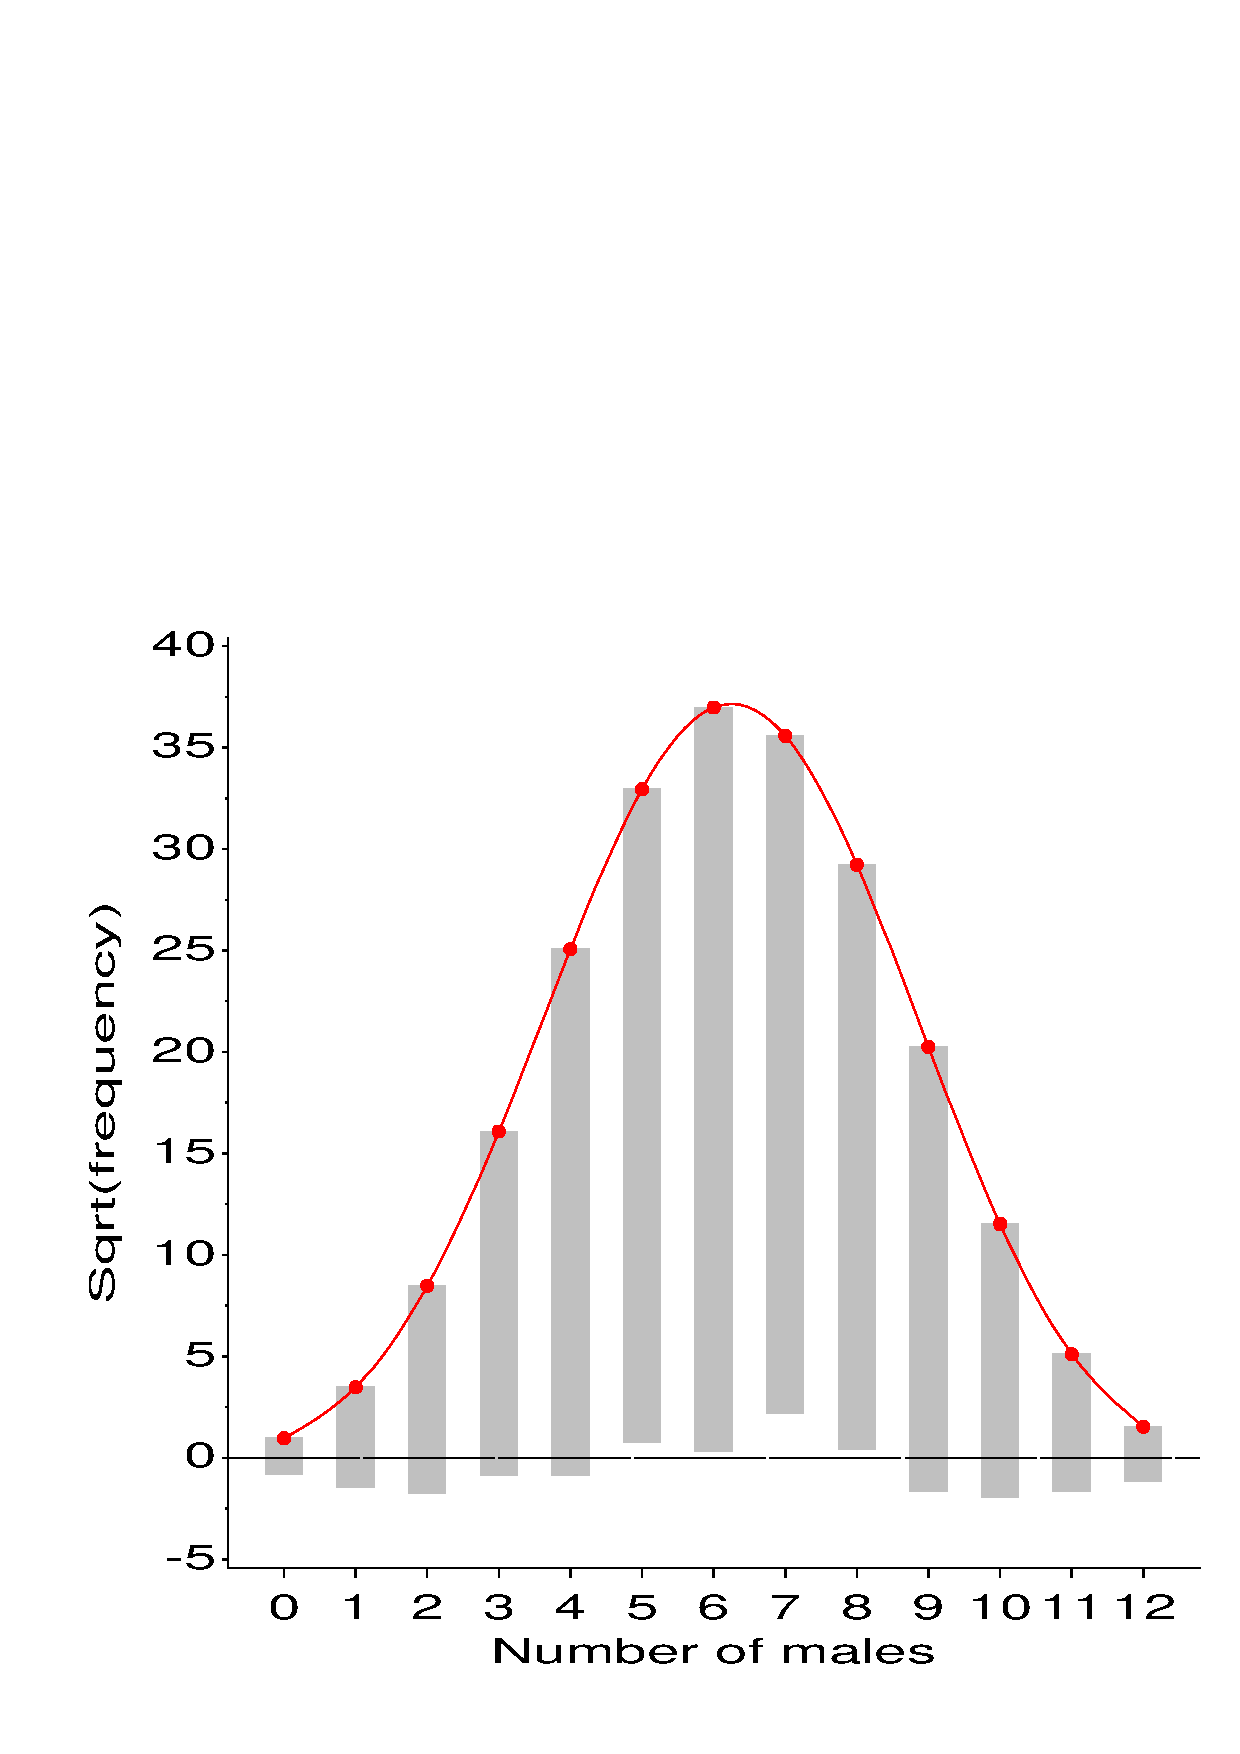
\includegraphics[width=1\linewidth]{saxony}\graphicsfile{ch2/fig/saxony.eps}{}
 \end{minipage}%
 \hfill
 \begin{minipage}[c]{.33\linewidth}
  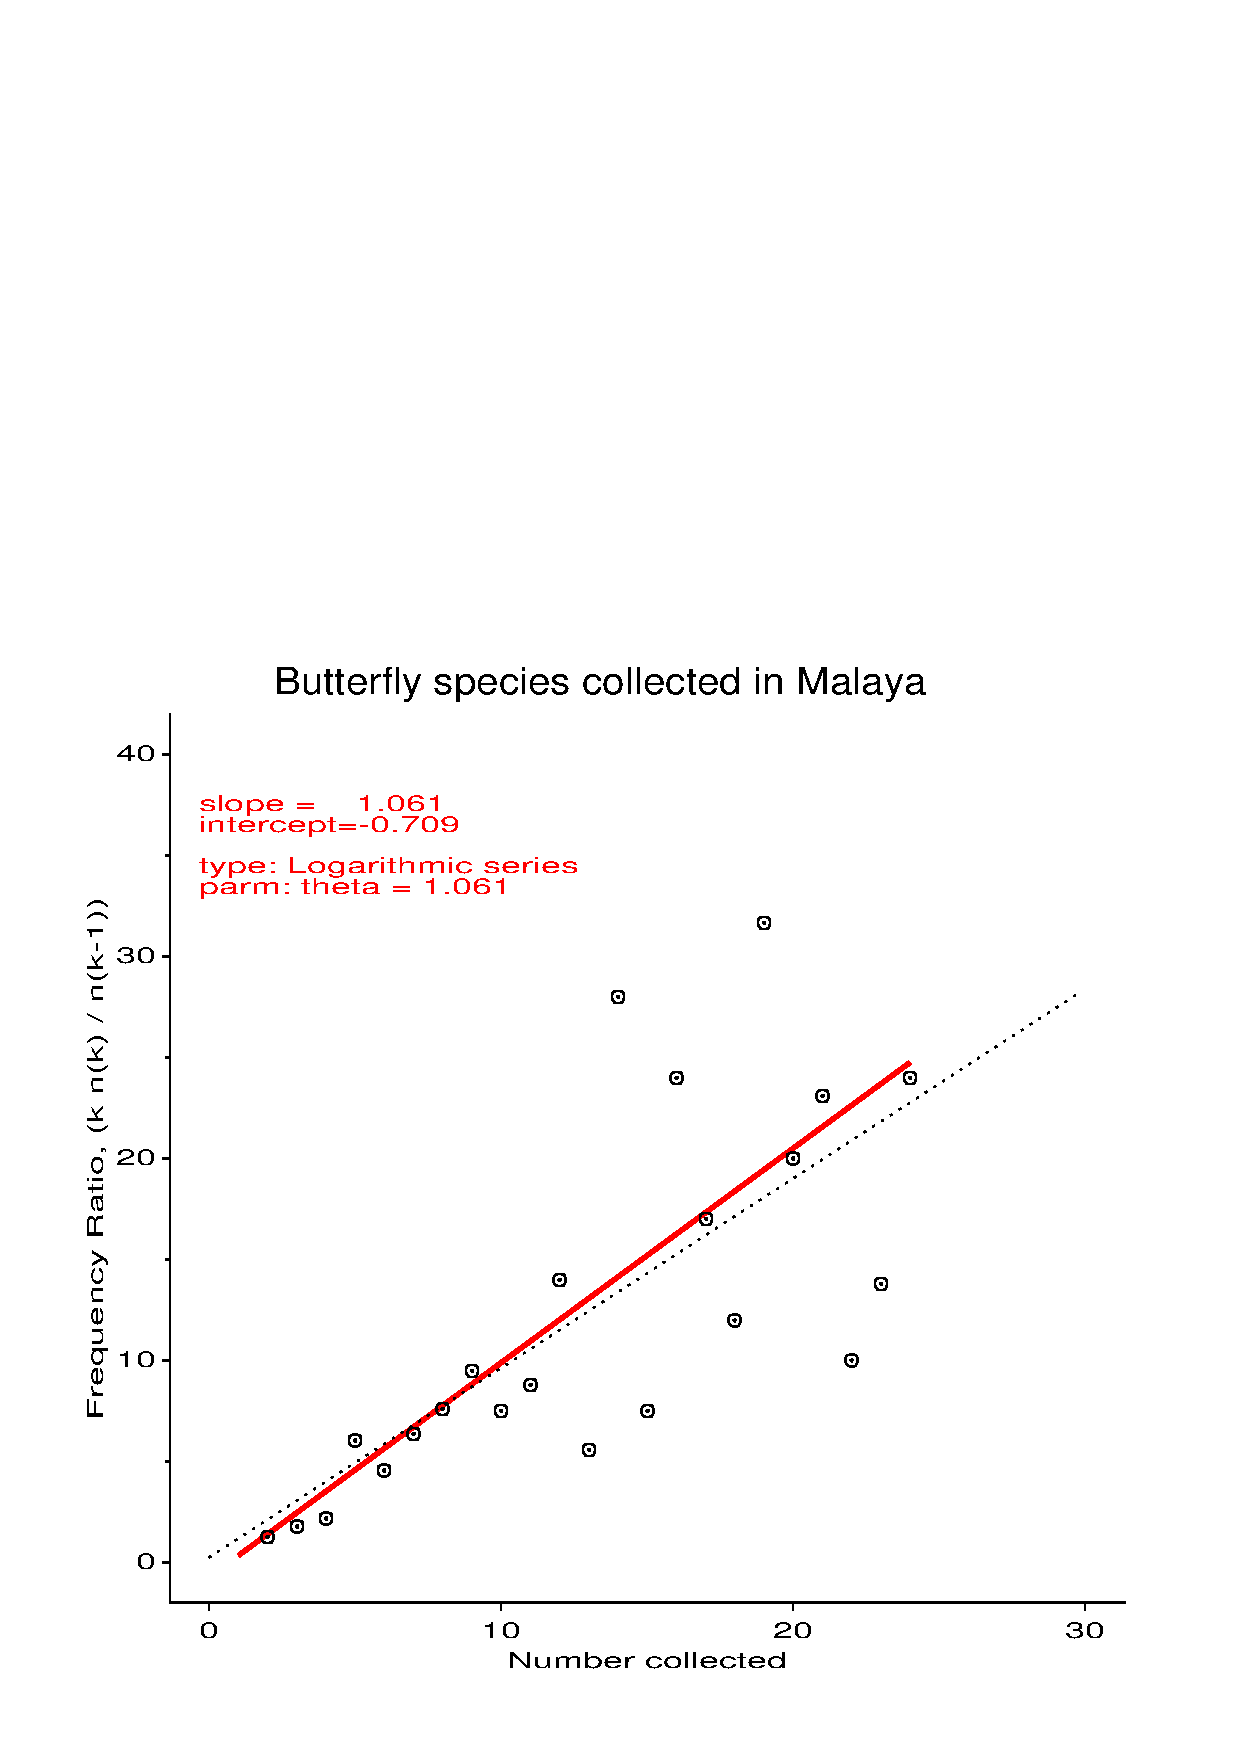
\includegraphics[width=1\linewidth]{orddemo3}\graphicsfile{ch2/fig/orddemo3.eps}{}
 \end{minipage}
 \hfill
 \begin{minipage}[c]{.33\linewidth}
  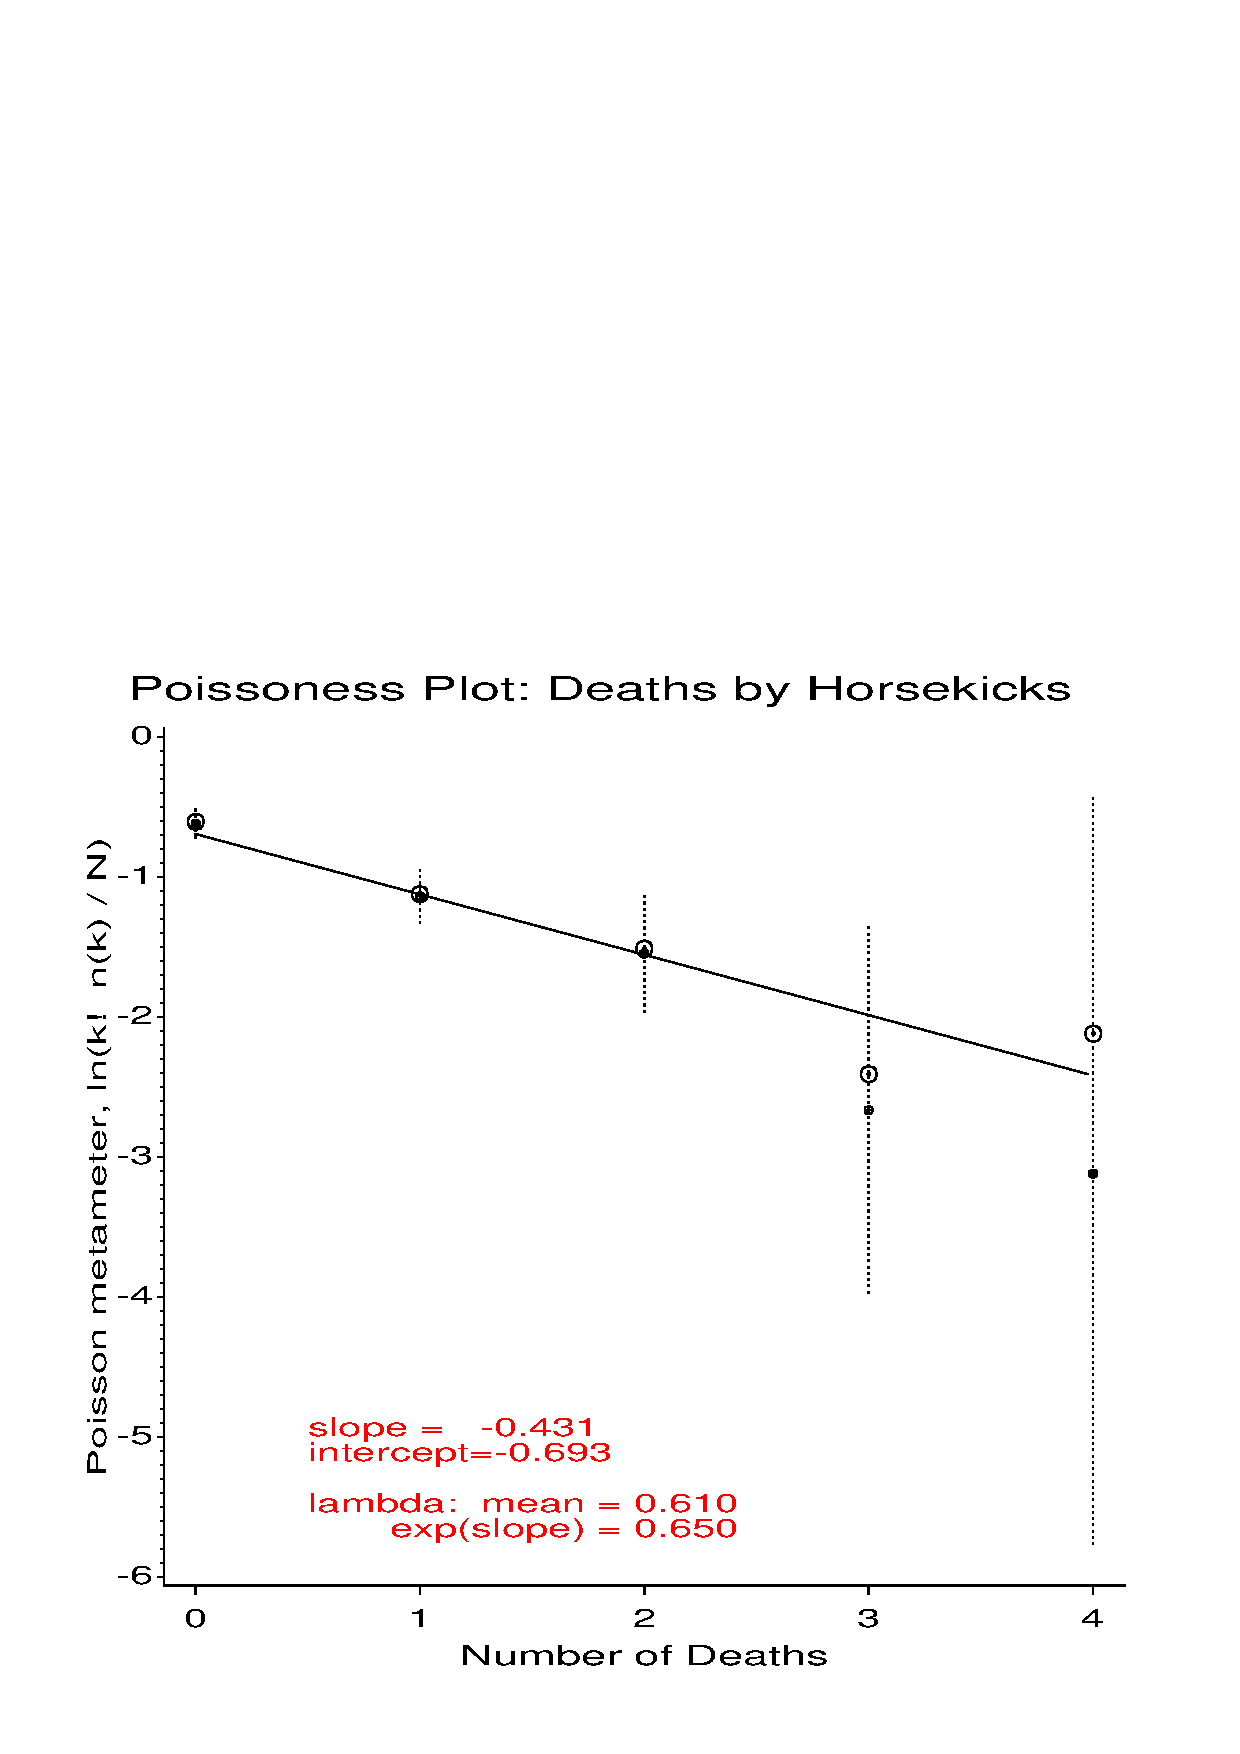
\includegraphics[width=1\linewidth]{poisdemo1}\graphicsfile{ch2/fig/poisdemo1.eps}{}
 \end{minipage}
\end{center}


\begin{quote}
{\Large
Logistic regression describes the relation between 
a discrete response, often binary, and a set of explanatory variables.
Smoothing techniques are often crucial in visualizations for such
discrete data.  The fitted model provides both inference and
prediction, accompanied by measures of uncertainty.  Diagnostic
plots help us to detect influential observations which may distort
our results.
}
\end{quote}
\minitoc
\clearpage

\section{Introduction}
\epigraph{In scientific thought we adopt the simplest theory which will explain
all the facts under consideration and enable us to predict new facts of
the same kind. The catch in
this criterion lies in the world ``simplest.''}
{J. B. S. Haldane, \emph{Possible Worlds}, 1927.}
Previous chapters have been concerned primarily with simple,
exploratory methods for studying the relations among categorical
variables and with testing hypotheses about their associations
through non-parametric tests and with overall goodness-of-fit
statistics.

This chapter begins our study of model-based methods for the analysis
of discrete data.  These models differ from those we have examined
earlier primarily in that they consider \emph{explicitly} an
assumed probability distribution for the observations, and make
clear distinctions between the systematic component, which is
explained by the model, and the random component, which is not.
In this chapter we consider models for a binary response,
such as ``success'' or ``failure'',
or the number of ``successes'' in a fixed number of ``trials'',
where we might reasonably assume a binomial distribution for the
random component.

This model-fitting approach has several advantages.
Inferences for the model parameters include both hypothesis tests
and confidence intervals.  The former help us to assess which
explanatory variables affect the outcome;  the size of the estimated
parameters and the widths of their confidence intervals help us to
assess the strength and importance of these effects.
Finally, the predicted values obtained from the model
smooth the discrete responses, allow predictions for unobserved
values of the explanatory variables, and
provide important means to interpret the fitted relationship graphically.

The first section discusses models for a binary response, of which the most
widely used is the logistic regression model.
\secref{sec:logist-quant} illustrates these models for
a quantitative predictor and 
describes the construction and use of graphical displays.
\secref{sec:logist-qual} extends these models to qualitative predictors,
and the general, multiple logistic regression model is discussed in \secref{sec:logist-mult}.
For interpreting and understanding the results of a fitted model,
I emphasize plotting predicted probabilities and predicted log odds.
Individual observations sometimes exert great influence on a fitted model.
Some measures of influence and diagnostic plots are illustrated in
\secref{sec:logist-infl};
in \secref{sec:logist-poly}, I develop several approaches to
modelling a multi-category (polytomous) response,
while \secref{sec:logist-btl} shows how a classic model for
paired comparisons data may be handled by logistic regression.
A final section (\secref{sec:logistic-power})
illustrates how to calculate and graph statistical power in relation
to sample size for two simple cases of logistic regression.

The logistic regression model is also discussed and illustrated with
SAS computations in \LRE,
\citet[\C 8--9]{Stokes-etal:95},
\citet{Allison:99} and \citet[\C 3]{Zelterman:99},
all of which are useful companions to this book.
\citet{Agresti:90}, \citet{Collett:91}, and \citet{Fox:97} provide a more detailed treatment
of the statistical background than I do here.

\section{The logistic regression model}\label{sec:logist-model}

The logistic regression model
describes the relationship between a categorical outcome variable,
the ``response'', and a set of explanatory variables.
The response variable is often \boldital{dichotomous}, although
extensions to the model permit multi-category,
\boldital{polytomous} outcomes, discussed in
\secref{sec:logist-poly}.
The explanatory variables may be continuous or (with dummy variables)
discrete.

For a binary response, $Y$, and a continuous explanatory variable, $X$,
we may be interested in modeling the probability of a successful
outcome, which we denote $\pi(x) \equiv \Pr(Y=1 \given X=x)$.
That is, at a given value $X = x$, we imagine that there is a
binomial distribution of the responses, $\Bin( \pi(x), n_x )$.

We might contemplate a simple linear regression model for $\pi(x)$,
\begin{equation*}%\label{eq:logit0}
E ( Y ) = \pi(x) =
\alpha + \beta x \comma
\end{equation*}
which we could fit by ordinary least squares (\PROC{REG}, for example).
However, such a model (called the \emph{linear probability model}),
has the serious defect that it yields predicted probabilities $\hat{\pi}(x) < 0$
for sufficiently small $x$ and $\hat{\pi}(x) > 1$ for sufficiently large $x$
(assuming $\beta > 0$).

One way around this difficulty is to re-specify the model so that a
transformation of $\pi$ has a linear relation to $x$, and that transformation
keeps $\hat{\pi}$ between 0 and 1 for all $x$.
A particularly convenient choice gives the linear logistic regression model, which posits a linear relation between
the log odds, or \glossterm{logit} of this probability and $X$,
\begin{equation}\label{eq:logit1}
\logit[ \pi(x) ] \equiv
\log \left( \frac{\pi(x) }{1-\pi(x) } \right) =
\alpha + \beta x \period
\end{equation}
When $\beta > 0$, $\pi (x)$ and the log odds increase as $X$ increases;
when $\beta < 0$ they decrease with $X$.
From \eqref{eq:logit1} we see that the odds of a favorable response
can be expressed as
%
\begin{equation}\label{eq:logit2}
\mbox{odds}(Y=1) \equiv \frac{\pi(x) }{1-\pi(x) }  =
\exp (\alpha + \beta x) = e^{\alpha} ( e^{\beta} )^x \: ,
\end{equation}
%
a multiplicative model for the odds.
So, under the logistic model,
\begin{itemize*}
\item $\beta$ is the change in the log odds associated with a unit
increase in $x$.
The odds are multiplied by $e^{\beta}$ for each unit increase in $x$.
\item $\alpha$ is log odds at $x=0$; $e^{\alpha}$ is the odds of
a favorable response at this $x$-value
(which may not have a reasonable interpretation if $X=0$ is far from
the range of the data).
\end{itemize*}

Rearranging terms in \eqref{eq:logit2}, the logistic regression model may also be formulated as a direct relationship for the probability of success,
\begin{equation}\label{eq:logit3}
\pi(x) = \frac{\exp (\alpha + \beta x)}{1+ \exp (\alpha + \beta x) } \:.
\end{equation}
This expression may look complex, but, the numerical results are
easy to interpret.
We will find it most convenient for plotting and understanding results
from logistic regression to express fitted values on the scale of
probabilities.

It may also help to know that, on the scale of probabilities, the 
slope of the relationship between $\pi(x)$ and $x$ is
$\beta \pi (1-\pi)$, so you can also interpret the slope in
\eqref{eq:logit1} as a change in probability of success for a unit
change in $x$. But the numerical value depends on the probability itself.
This expression is at its maximum when $\pi = 0.5$.  However
it doesn't change very much within the range $0.2 < \pi < 0.8$, as we
will see in the following example.

\begin{Example}[arthrit6]{Arthritis treatment}
\begin{table}[htb]
 \caption{Probabilities, Odds, and Logits for the Arthritis Treatment Data}\label{tab:arthlogit}
 \begin{center}
 \begin{tabular}{r@{ -- }l rrrrr}
 \hline
  \multicolumn{2}{c}{Age}
		       & Number &       & Observed   & Odds   & Observed \\ 
  \multicolumn{2}{c}{Group} 
             & Better & Total & $\Pr\{\mbox{Better}\}$ & Better & Logit \\ \hline
  23  &  31  &    2  &   8  &  0.250  &  0.333  &  -1.099 \\ 
  32  &  41  &    4  &   9  &  0.444  &  0.800  &  -0.223 \\ 
  44  &  48  &    2  &   8  &  0.250  &  0.333  &  -1.099 \\ 
  49  &  53  &    0  &   7  &  0.000  &  0.000  &  . \\ 
  54  &  57  &    9  &  12  &  0.750  &  3.000  &   1.099 \\ 
  58  &  58  &    2  &   3  &  0.667  &  2.000  &   0.693 \\ 
  59  &  61  &    7  &  11  &  0.636  &  1.750  &   0.560 \\ 
  62  &  63  &    4  &   8  &  0.500  &  1.000  &   0.000 \\ 
  64  &  67  &    5  &   9  &  0.556  &  1.250  &   0.223 \\ 
  68  &  74  &    7  &   9  &  0.778  &  3.500  &   1.253 \\ 
 \hline
 \end{tabular}
 \end{center}
\end{table}

In \chref{ch:twoway} we examined the data
on treatment for rheumatoid arthritis.
In addition to sex and treatment, the data (see \datref{dat:arthrit})
gives the age of each patient in this study.
Although the response has three categories (none, some, or marked
improvement), for now we consider whether the patient showed any
improvement at all, defining the event ``better'' to be some or
marked improvement.

Because age is continuous, it is difficult to see how the probability of
a better response varies with age.
\tabref{tab:arthlogit} summarizes these data
by dividing the patients into 10 decile groups based on age.%
\footnote{The ``total'' numbers are unequal because of ties.}
We see that for those in the youngest age group the observed
$\Pr\{\textrm{Better}\} = 2/8 = 0.25$, so the odds of a better response
is $0.25 / 0.75 = \frac{1}{3}$;  for those in the 62--63 age range,
half improved, so the odds = 1.  The log odds has the value 0 here.
Thus positive (negative) logits correspond to probabilities greater than
(less than) $\frac{1}{2}$.

You can see that the probabilities of a better response
and the logits tend to increase
with age.  Thus, we would expect to find $\beta > 0$ in Eqn.~\eqref{eq:logit1}.
Also note that when the probability is defined as
the observed number divided by the total in a group, the logit is
undefined when the observed probability is 0 or 1.
We improve on this below.

\figref{fig:logist1c1} shows a plot of the (0/1) variable \texttt{better}
against age.  (The programming for such plots is described in
\secref{sec:logist-quantp}.)
Also shown is the predicted probability from a logistic
regression (solid blue curve) and the upper and lower 95\% confidence
band for this predicted probability (dashed blue curves).
For comparison, we also show the result of a linear regression of
the (0/1) variable on age (red line) and its 95\% confidence band.
The two sets of curves are fairly similar, except in the extremes.
\begin{figure}[htb]
  \centering
  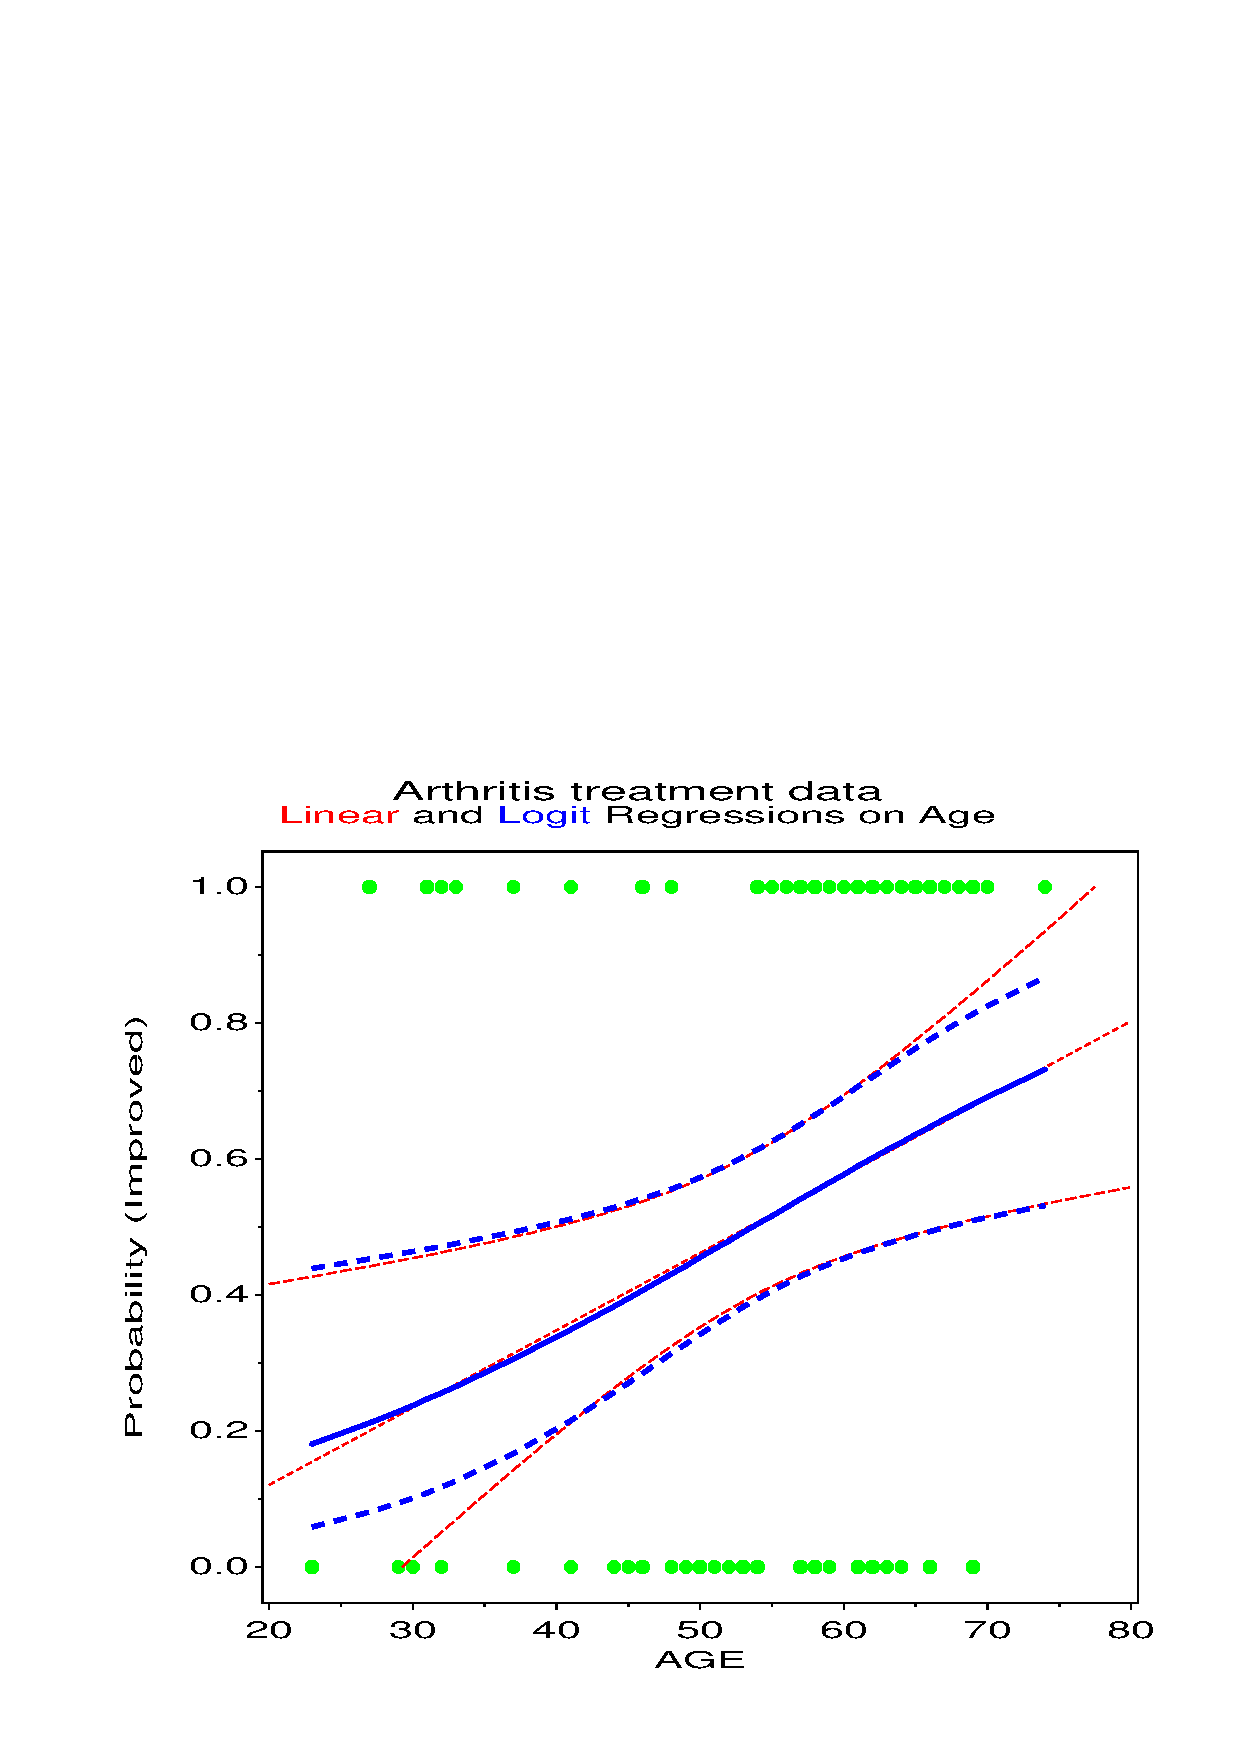
\includegraphics[scale=.7]{ch6/fig/logist1c1}
  \caption[Arthritis treatment data, linear and logit regressions on age]%
  {Arthritis treatment data, linear and logit regressions on age.  The curves show predicted probabilities of
improvement and 95\% confidence bands.
The points show the observations.  Except in the extremes, the linear
and logistic models give very similar predicted values; the confidence bounds
differ more.}%
  \label{fig:logist1c1}
\end{figure}

The relevant portion of the output is shown below.  The parameter estimates
are $\alpha = -2.642$, and $\beta = 0.0492$.  So, the estimated odds of
a better response are multiplied by $e^{\beta} = \exp(0.0492) = 1.05$
for each one year increase in age.  Equivalently, you can think of this
as a 5\% increase per year (using $100 (e^{\beta} -1)$ to convert).
Over 10 years, the odds are multiplied by $\exp(10 \times 0.0492) = 1.64$,
a 64\% increase.
\begin{output}
                  Analysis of Maximum Likelihood Estimates

            Parameter Standard    Wald       Pr >    Standardized    Odds
Variable DF  Estimate   Error  Chi-Square Chi-Square   Estimate     Ratio

INTERCPT 1    -2.6421   1.0732     6.0611     0.0138            .    .
AGE      1     0.0492   0.0194     6.4733     0.0110     0.346714   1.050
\end{output}
\end{Example}

\subsection{Plotting a discrete response: the \macro{LOGODDS}}\label{sec:logist-logodds}

It is sometimes difficult to understand how a binary response can give
rise to a smooth, continuous relationship between the predicted response
and an explanatory variable, particularly when the predictor is
continuous.
Thus, in \figref{fig:logist1c1} you can see the (0/1) responses
and the fitted relation, but it takes some effort to see that
the observation points determine that relation.
Another problem is that the age variable is not strictly continuous ---
it was recorded in whole years --- so there may be considerable
overplotting of the observation points in such a graph.

%% two subfig side-by-side
\begin{figure}[htb]
 \begin{minipage}[t]{.49\linewidth}
  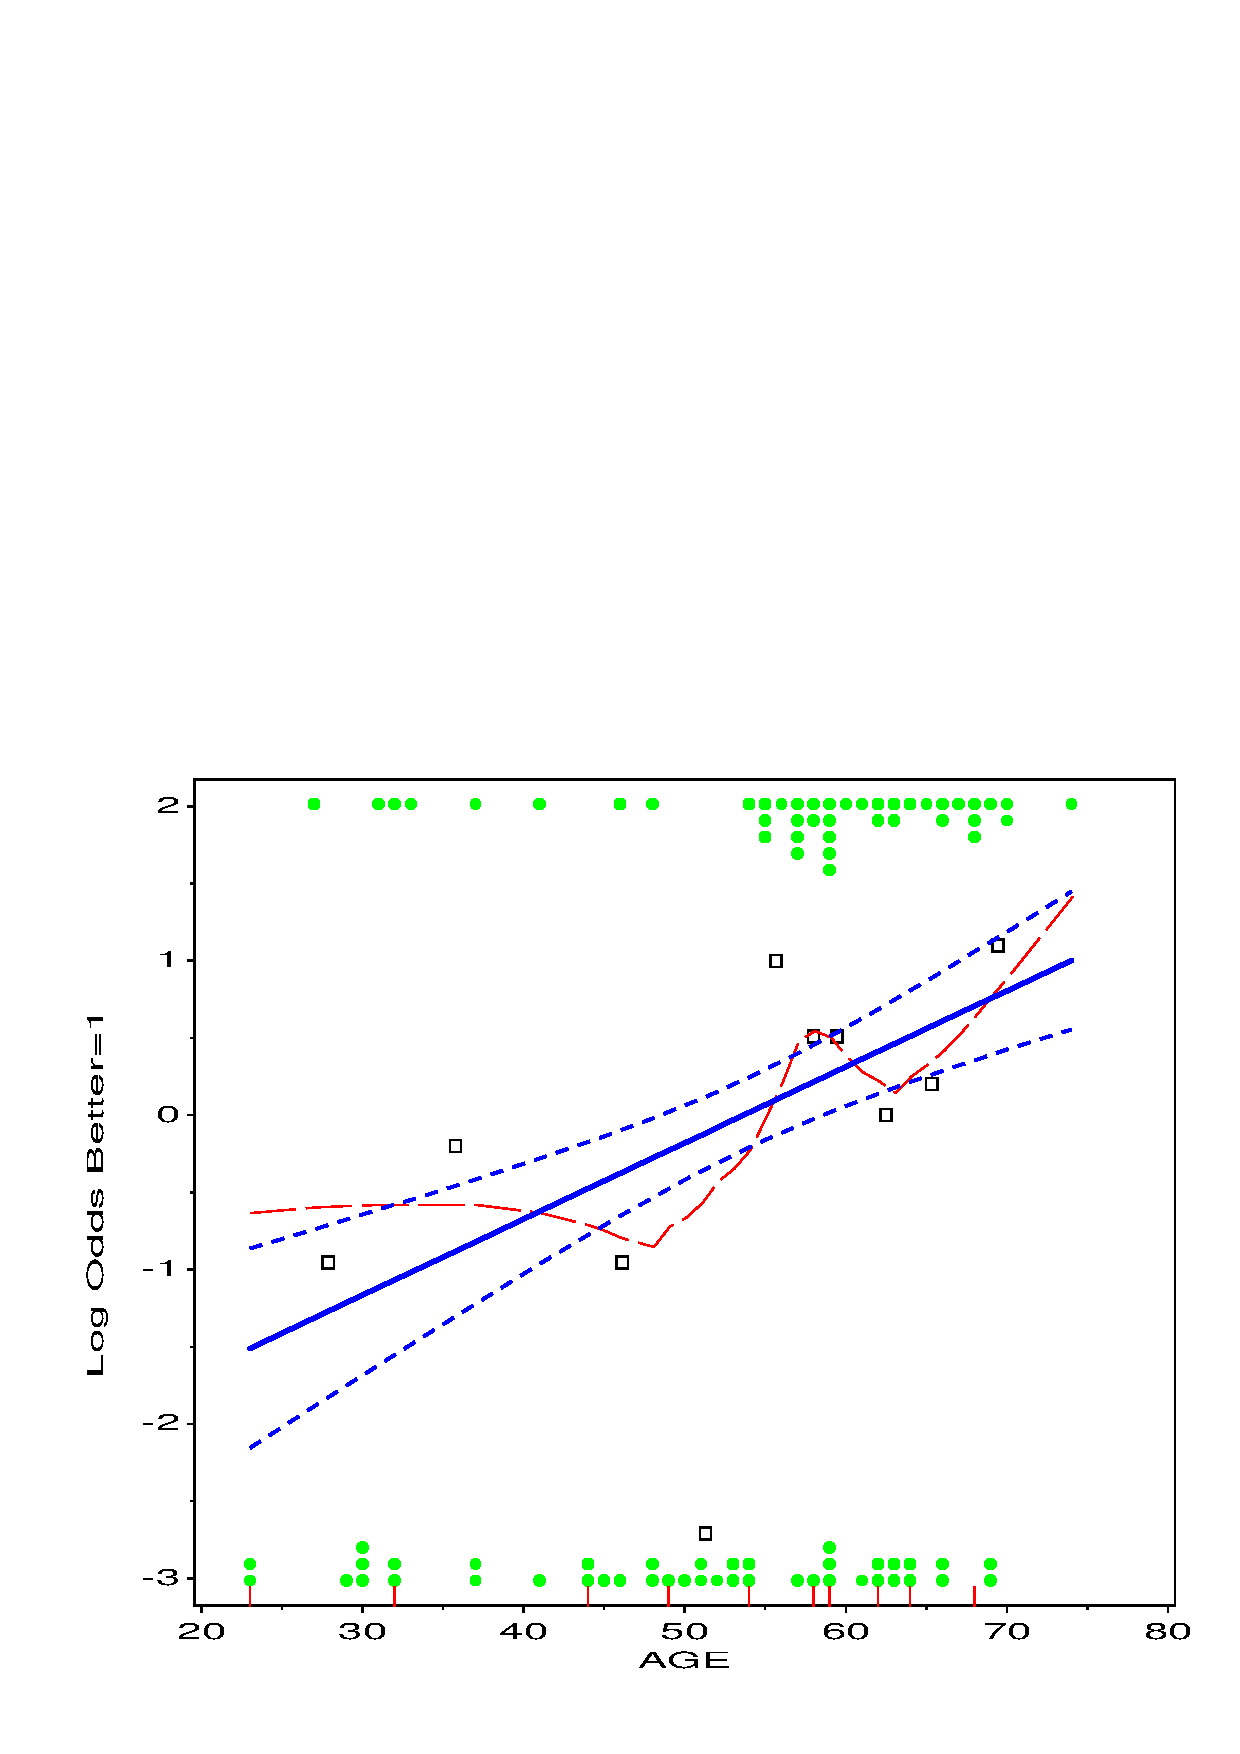
\includegraphics[width=1\linewidth]{ch6/fig/logoddt1}
 \end{minipage}%
 \hfill
 \begin{minipage}[t]{.49\linewidth}
  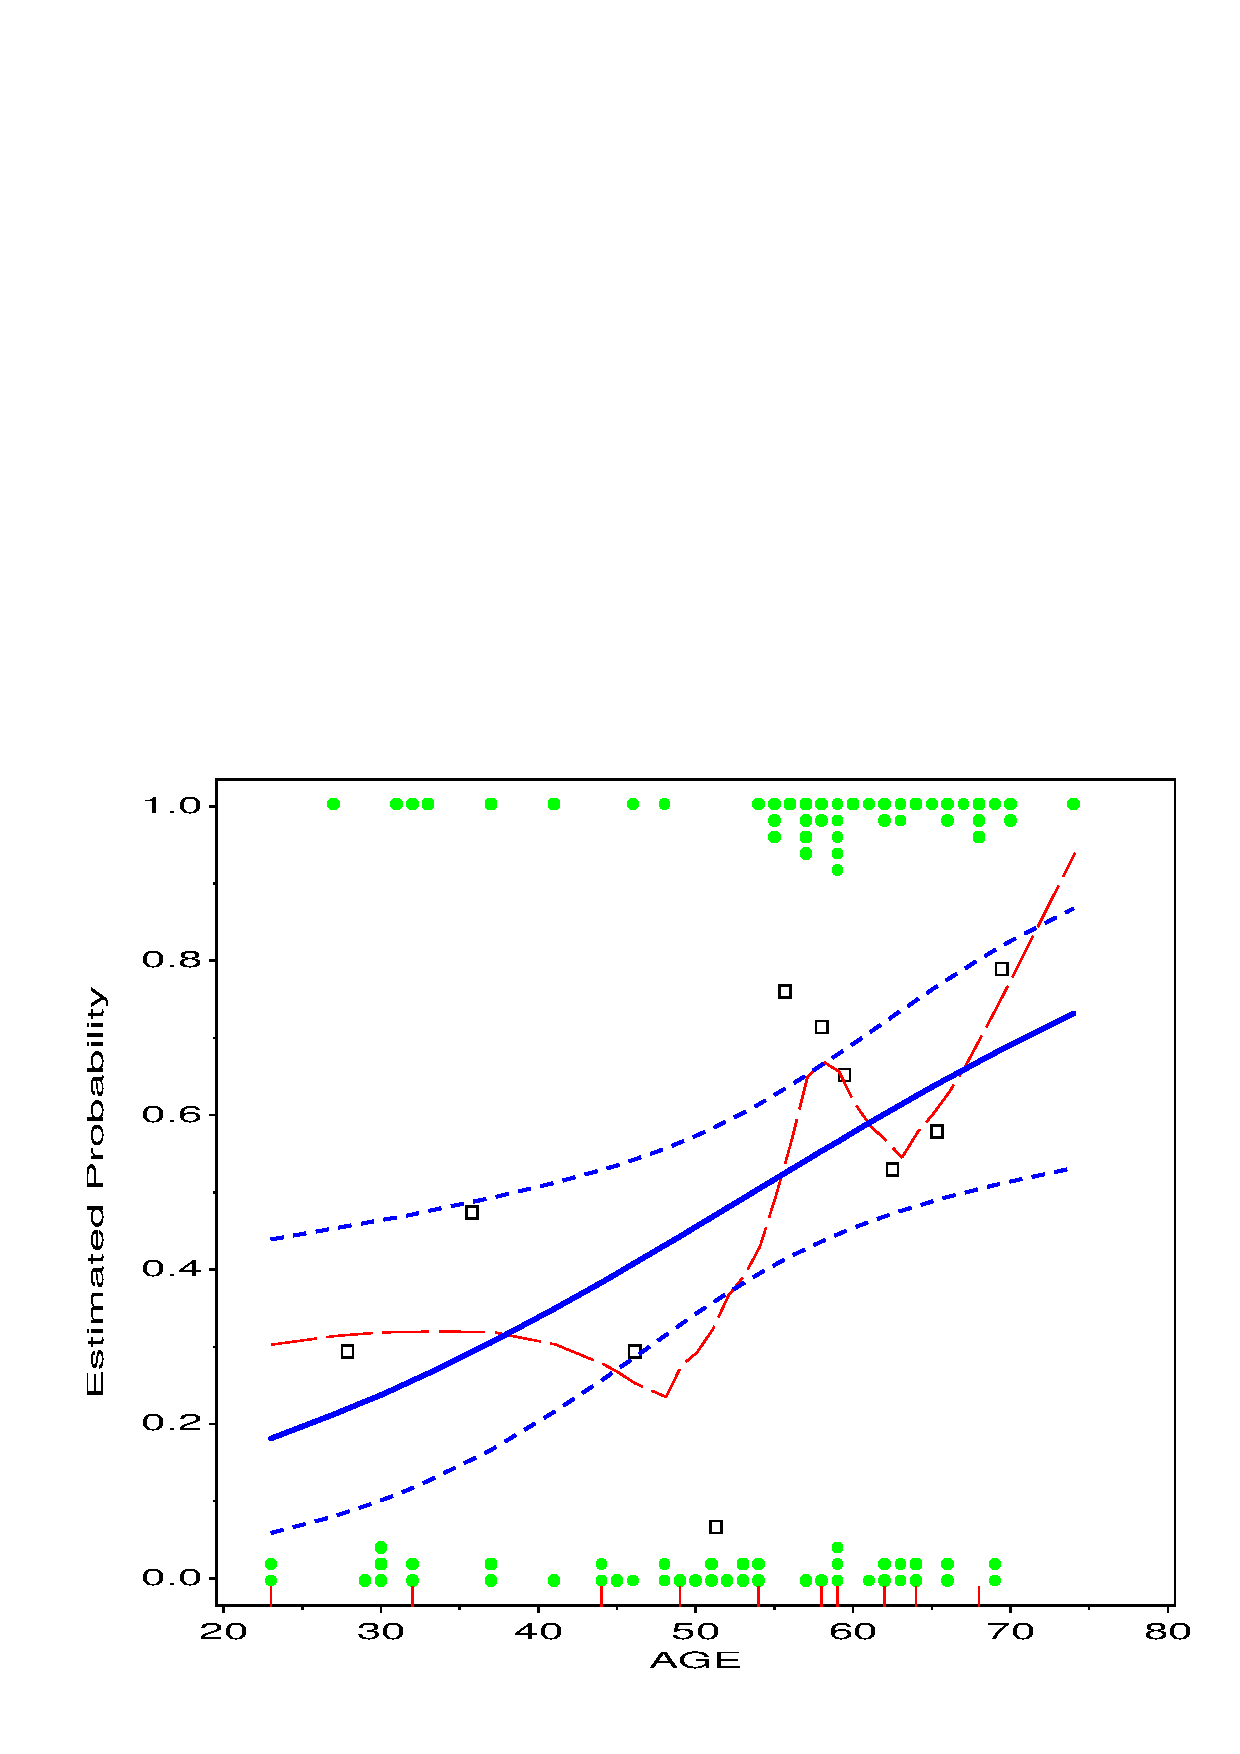
\includegraphics[width=1\linewidth]{ch6/fig/logoddt2}
 \end{minipage}
 \caption[Empirical log-odds and probability plots for arthritis treatment data]{Empirical log-odds and probability plots for arthritis treatment data.
 The observed responses are plotted as stacked points at the top and bottom of the figures.  The squares show the empirical sample logits, and the analogous adjusted sample probabilities.}\label{fig:logoddt}
\end{figure}

It is helpful, therefore, to plot the observed sample logits or
sample probabilities against $X$, together with the observations
(in a way which avoids overplotting), and the fitted relationships,
as we do in \figref{fig:logoddt}.
Suppose we group the observations into some number of intervals,
as in \tabref{tab:arthlogit},
and let $n_i$ denote the number of observations in the $i$th
interval, of which $y_i$ are successful events.

Then, the observed probability is $p_i = y_i / n_i$ in interval $i$,
and the sample logit is
$\log[ p_i / (1 - p_i) ] = \log[ y_i / (n_i - y_i)]$.
But as we saw in \tabref{tab:arthlogit}, the logit is not defined
when $y_i =0$, or when $y_i = n_i$.
We get around this difficulty by substituting the
\boldital{empirical logit},
\begin{equation*}
 \log \left( \frac{y_i + \frac12}{n_i - y_i + \frac12} \right)
 \comma
\end{equation*}
which is also a less biased estimator of the true logit.  Analogously, in
a plot of probabilities against $X$, we use the adjusted value
$ (y_i + \frac12) / (n_i - y_i + \frac12)$.

An alternative to grouping the observations into fixed intervals is to
imagine a sliding window, wide enough to contain a given fraction,
$f$ of the points, moving from left to right across the plot.
At each position of the window,  calculate a smoothed, locally weighted
average of the binary $y$ values within the window using the
\glossterm{lowess} scatterplot smoothing algorithm
\citep{Cleveland:79} (without robustness iterations).
This gives a smooth, nonparametric regression for $\hat{p}_i$,
advocated by \citet{Landwehr-etal:84} and \citet{Fowlkes:87}.
\citet{Copas:83} discusses methods based on kernel density estimation
for smoothing binary data.

These plots are produced by the \macro{LOGODDS}, documented in
\macref{mac:logodds}.
Both plots in \figref{fig:logoddt}
were produced by these statements:
\begin{listing}
%include data(arthrit);
data arthrit;
   set arthrit;
   format better outcome.;
%logodds(data=arthrit, x=age, y=Better, ncat=10, smooth=0.5);
\end{listing}

The macro assumes a quantitative predictor and groups the observations
into the number of intervals specified by the \mparm{NCAT=}{LOGODDS}.
The lower limits of the intervals are shown by the short vertical lines
above the horizontal axis.
When the \mparm{SMOOTH=}{LOGODDS}  is specified, the \macro{LOWESS}
\citep[App. A1.9]{Friendly:91} using that value as the smoothing parameter,
$f$, and the smoothed nonparametric curve is drawn on the probability
plot.
With moderate sample sizes, as we have here, the lowess curve may be quite
variable, and of course ignores other explanatory variables.

Note that the fitted regression relation is linear on the scale of log odds
(cf. \eqref{eq:logit1})
but (slightly) non-linear on the scale of probabilities
(cf. \eqref{eq:logit3}).
Because most people find it easier to interpret probabilities than log odds,
it is often useful to make a single plot showing \emph{both} scales.

\subsection{Plotting a discrete response: Easy smoothing with \PROC{GPLOT}}\label{sec:logist-smooth}

For large \Dsets, extensive computations are required to calculate the lowess curve, because a weighted least squares regression is performed
for each observation.%
\footnote{In \sasver{7}, the \macro{LOWESS} uses the \proc{LOESS}
to perform the calculations, avoiding this difficulty.
In prior versions, use the \mparm{STEP=}{LOWESS} for large \Dsets.
The \mparm{STEP=}{LOWESS} sets a step size for successive
$x$ values.  When \pname{STEP>1}, the macro performs the regression at
every \pname{STEP}-th value of $x$, and uses predicted values from
    that regression for intermediate points.}
A simple alternative, which is often sufficient, is to use the
\pname{SM}\emph{nn} spline smoother provided by the
\pname{INTERPOL} option of the \stmt{SYMBOL}{GPLOT}.
The following example illustrates this technique and the importance
of smoothing.

\begin{Example}[titanic4]{Survival on the \emph{Titanic}}
The \emph{Titanic} data, discussed in \exref{ex:titanic},
included all passengers and crew, but categorized age as either
child or adult.
The data used here lists 1313 passengers by name, and includes the
actual age for 633 of these.
These data were derived from the ``Encyclopedia Titanica''
web site \citep{Hand:97}. They are based on the \emph{Titanic} Passenger List
originally published by \citet{Findlay:86}, and updated
by members of various \emph{Titanic} historical societies and internet
collaborators.
We examine here the relation of sex and class to actual age for these
passengers.

The \Dset\ \pname{titanic2} contains the variables
\pname{SEX}, \pname{CLASS},
\pname{AGE}, \pname{BOAT}, \pname{NAME}, and the 0/1 variable
\pname{SURVIVED}.
A simple, but effective plot of survival probability against age
for men and women is produced just by plotting
\pname{SURVIVED * AGE = SEX}, using \pname{INTERPOL=SM70}
on the \stmt{SYMBOL}{GPLOT}.
The numeric value in \pname{SM}\emph{nn} establishes the relative
weighting of criteria for approximating the points versus
smoothness, with larger values giving a smoother curve.
For binary responses, values in the range 50--90 appear to work
reasonably well.

The following statements produce the left panel in \figref{fig:psurvive12}.
(The \Dstp\ \pname{LABEL}, producing labels for the curves
is not shown to conserve space.)
Similar statements, plotting \pname{SURVIVED * AGE = CLASS}
produce the graph shown in the right panel of \figref{fig:psurvive12}.
\begin{listing}
proc sort data=titanic2;
   by age;

proc gplot data=titanic2;
   where (age^=.);
   plot survived * age = sex /
       anno=label vm=1 hm=1 vaxis=axis1 haxis=axis2 nolegend frame;
   symbol1 i=sm70 v=square   h=1.9 c=red;
   symbol2 i=sm70 v=triangle h=1.9 c=blue;
   axis1 order=(0 to 1 by .2) label=(a=90) offset=(3) value=(h=1.6);
   axis2 offset=(3) value=(h=1.6);
\end{listing}
%% two subfig side-by-side
\begin{figure}[htb]
 \begin{minipage}[t]{.49\linewidth}
  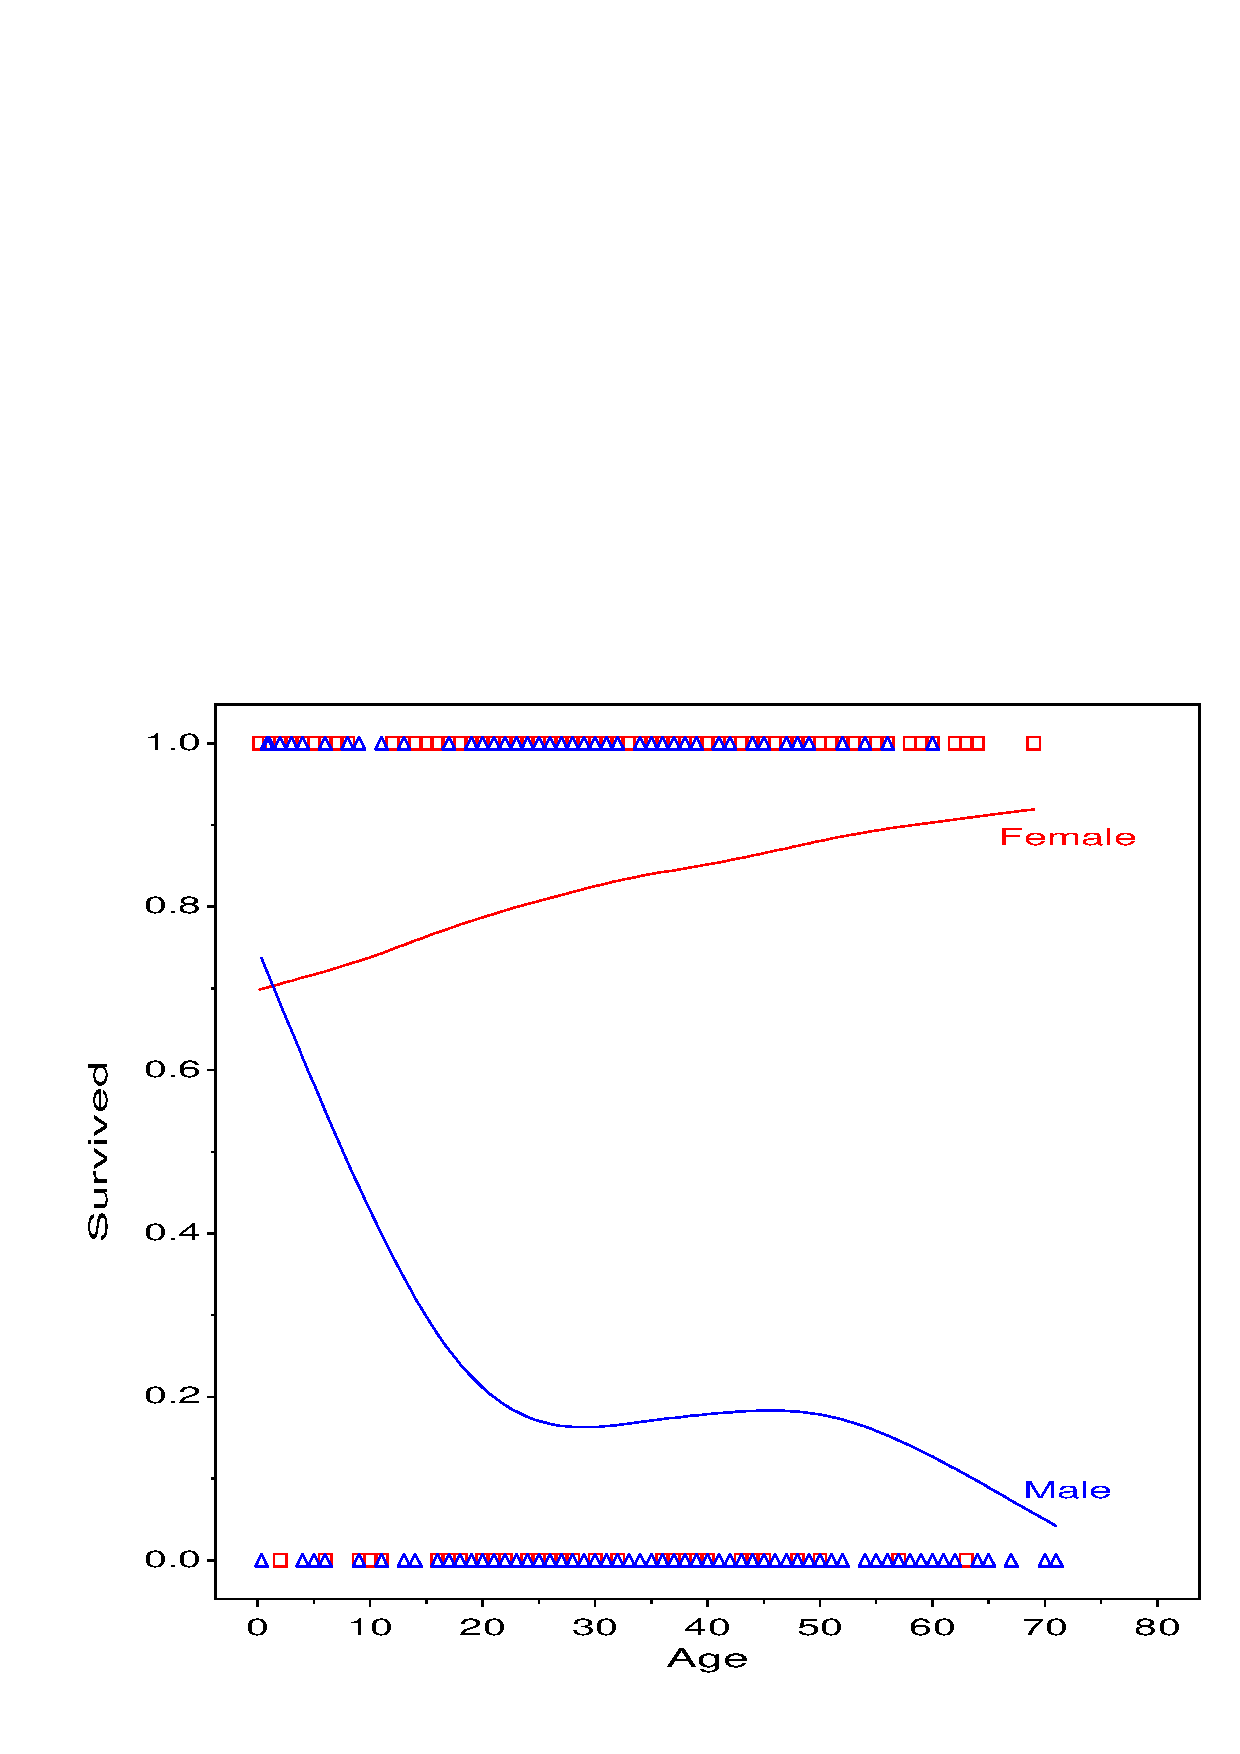
\includegraphics[width=1\linewidth]{ch6/fig/psurvive1}
 \end{minipage}%
 \hfill
 \begin{minipage}[t]{.49\linewidth}
  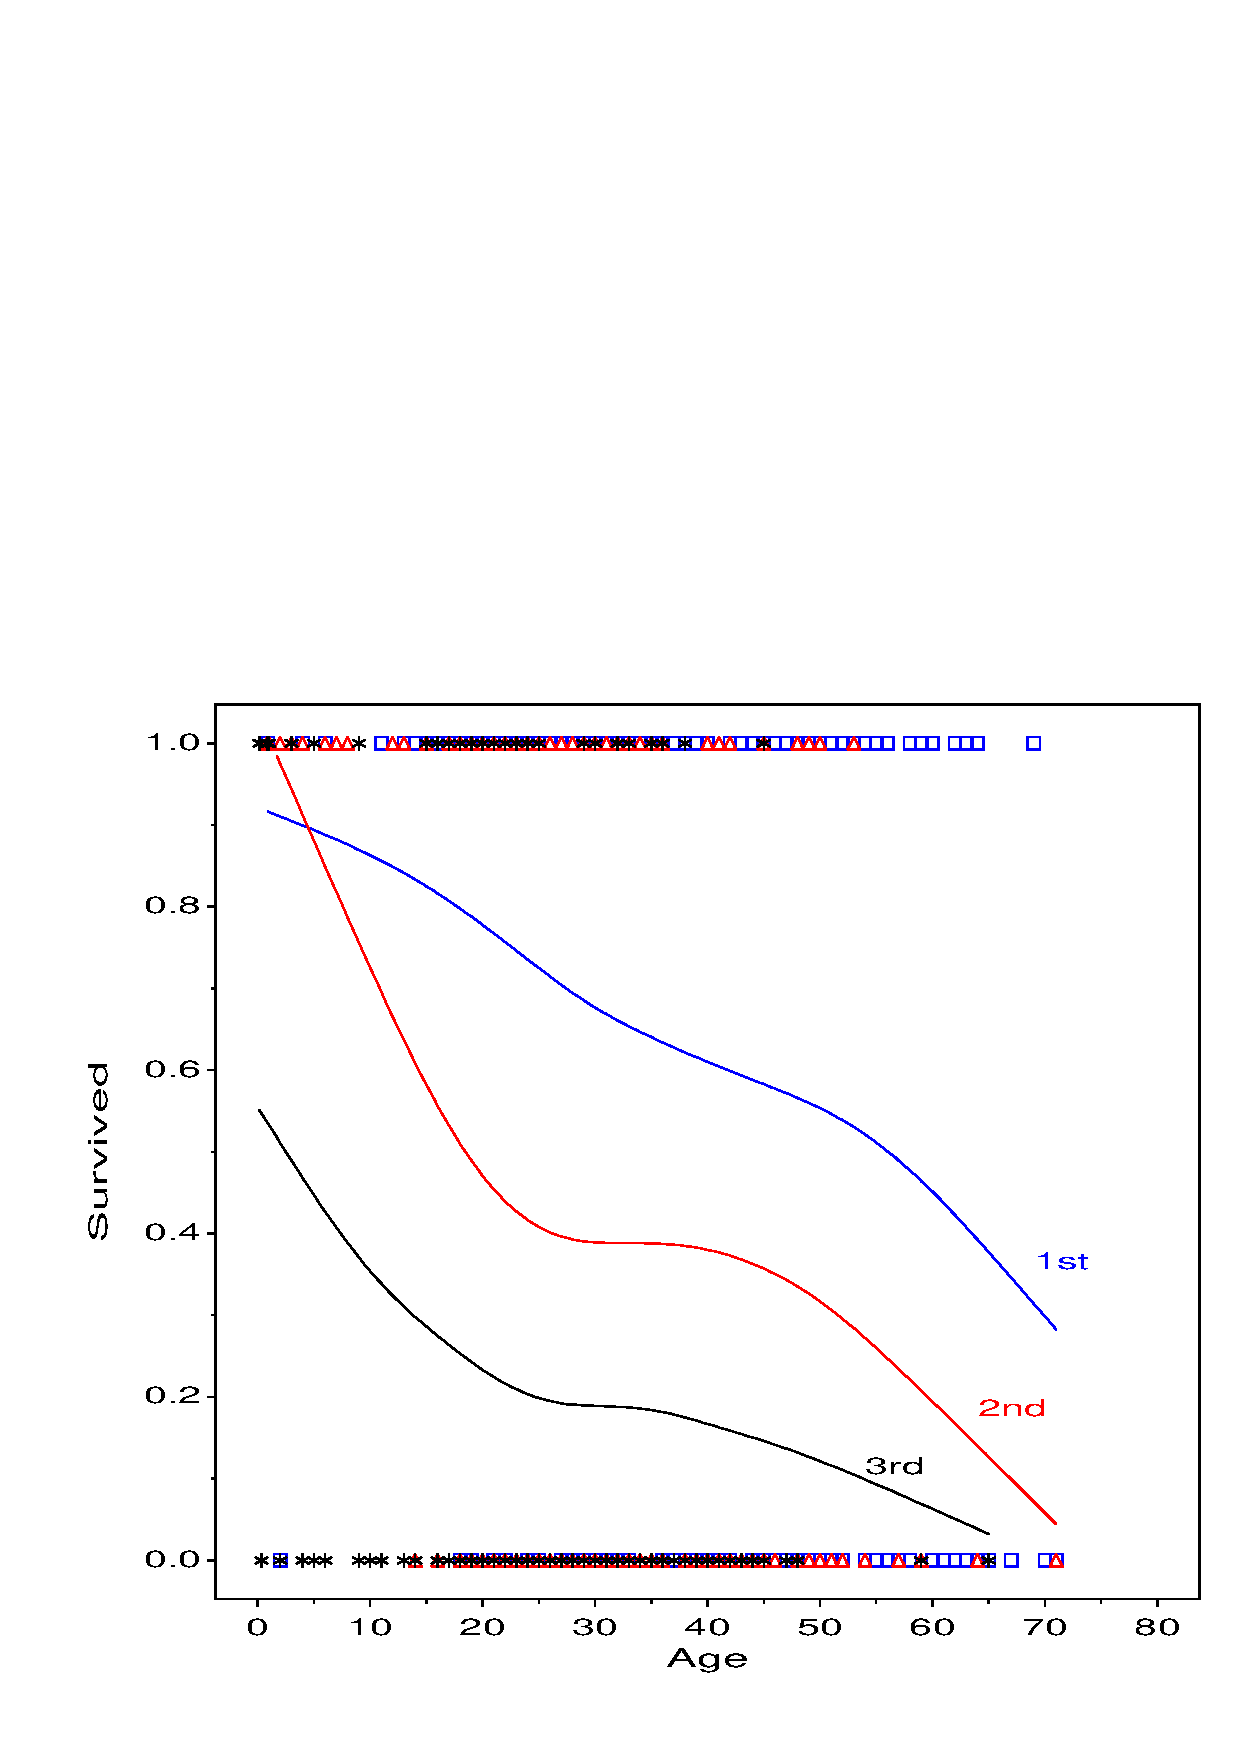
\includegraphics[width=1\linewidth]{ch6/fig/psurvive2}
 \end{minipage}
 \caption[Survival probability vs.\  age by sex (left), and by class (right), for passengers on the \emph{Titanic}]{Survival probability vs.\  age by sex, and by class, for passengers on the \emph{Titanic} whose age is recorded.
 Plot symbols show the individual observations.  These graphs are misleading because the effects of sex vary with class.}\label{fig:psurvive12}
\end{figure}

The actual binary responses, shown by the plotting symbols at
0 and 1 are not very informative here, because age is also discrete
(recorded to the nearest year) and many points are
overplotted.
Jittering the points would help somewhat, but would introduce some bias in
the smoothing.
The smoothed curves are highly suggestive, however,
and give a much more detailed view than our earlier analyses based
on the binary age classification.

For females, probability of survival increases steadily with age.
For males, however, the probability of survival drops precipitously with
age, levels off through middle age, then declines again for the
oldest men.
The smoothed curves in the right panel show similar cubic trends
with age for 2nd and 3rd class passengers.

It is tempting to speculate that these cubic curves reflect
preferential treatment towards boys and
greater chivalry, or perhaps decreased will to survive, on the part of
older men.
Such speculations would be dead wrong, however,
because they falsely assume that sex and class do not interact,
and that the distributions of age (as recorded in this data)
are roughly the same for all sex--class groups.

%% two subfig side-by-side
\begin{figure}[htb]
 \begin{minipage}[t]{.49\linewidth}
  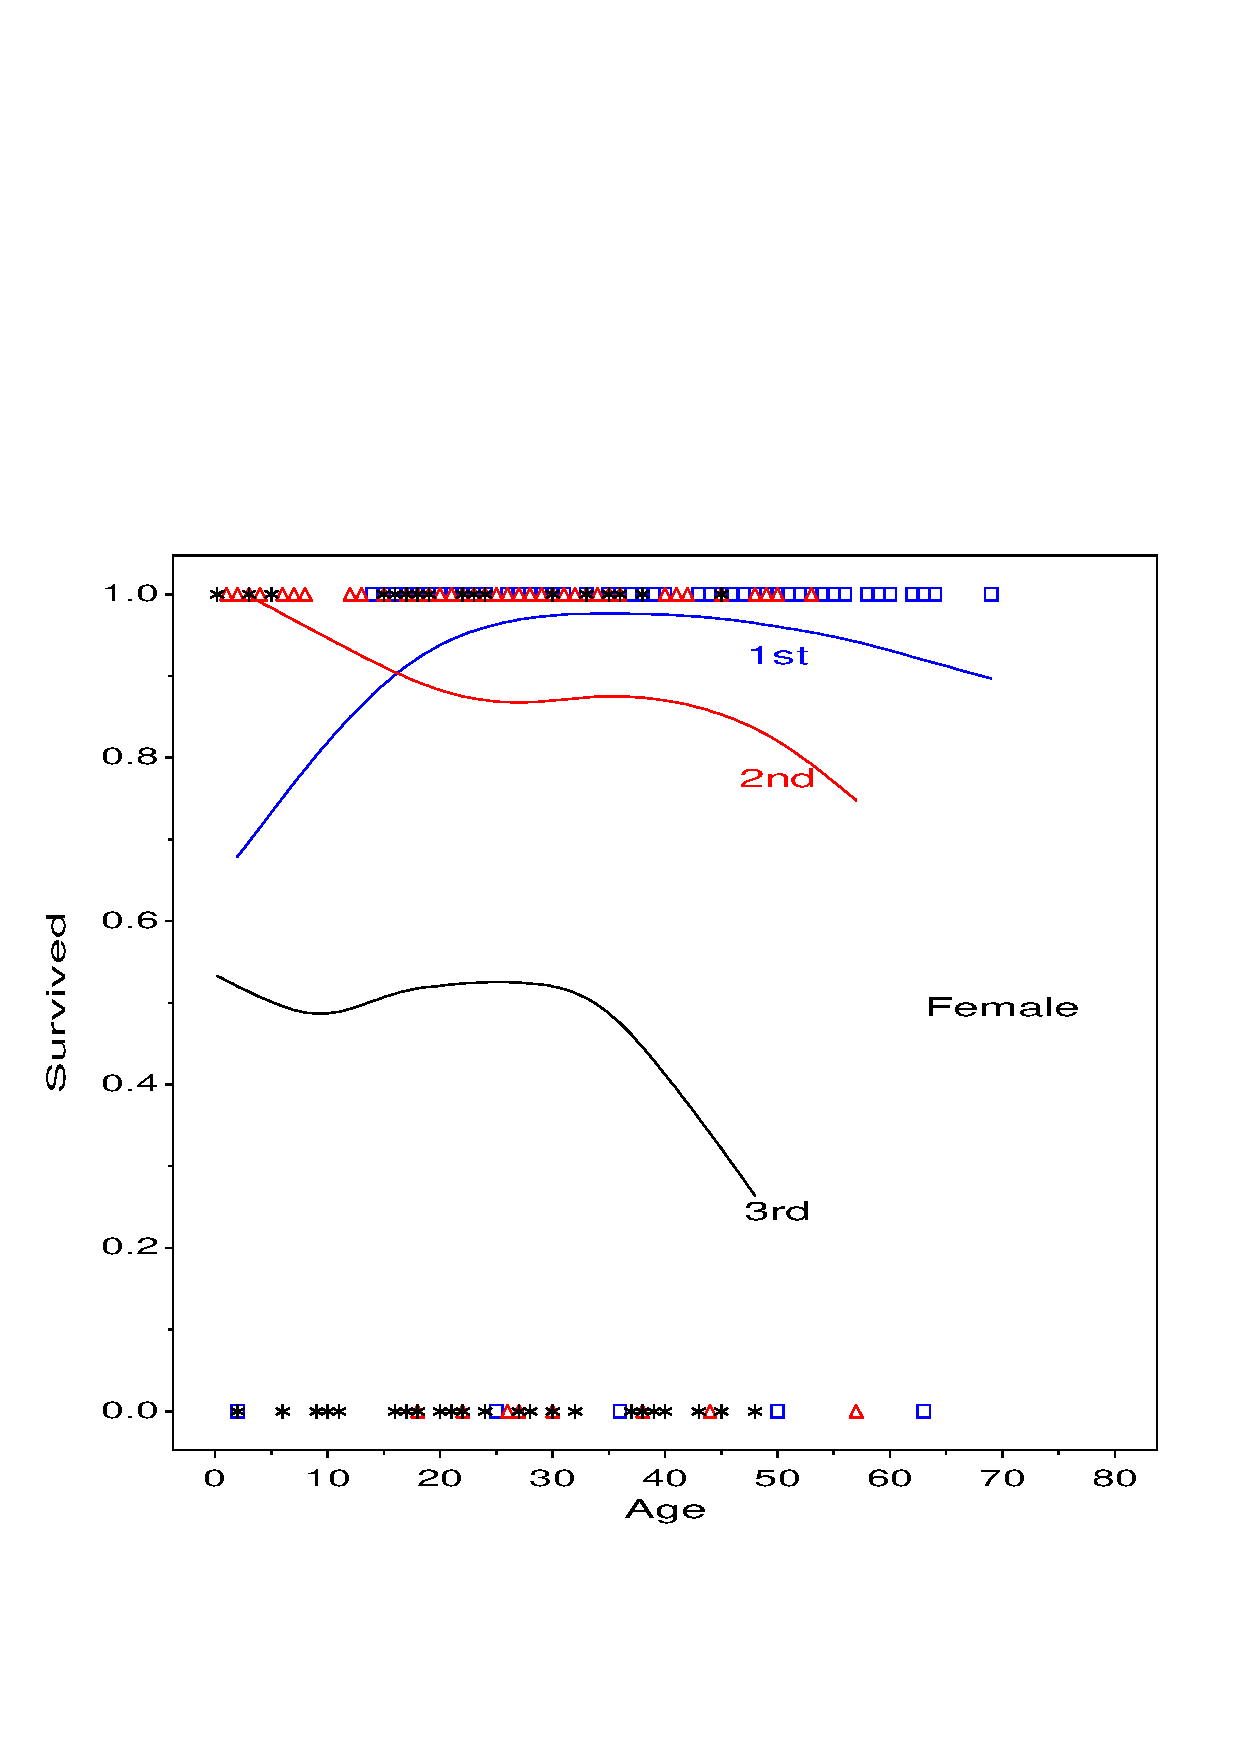
\includegraphics[width=1\linewidth]{ch6/fig/psurvive3}
 \end{minipage}%
 \hfill
 \begin{minipage}[t]{.49\linewidth}
  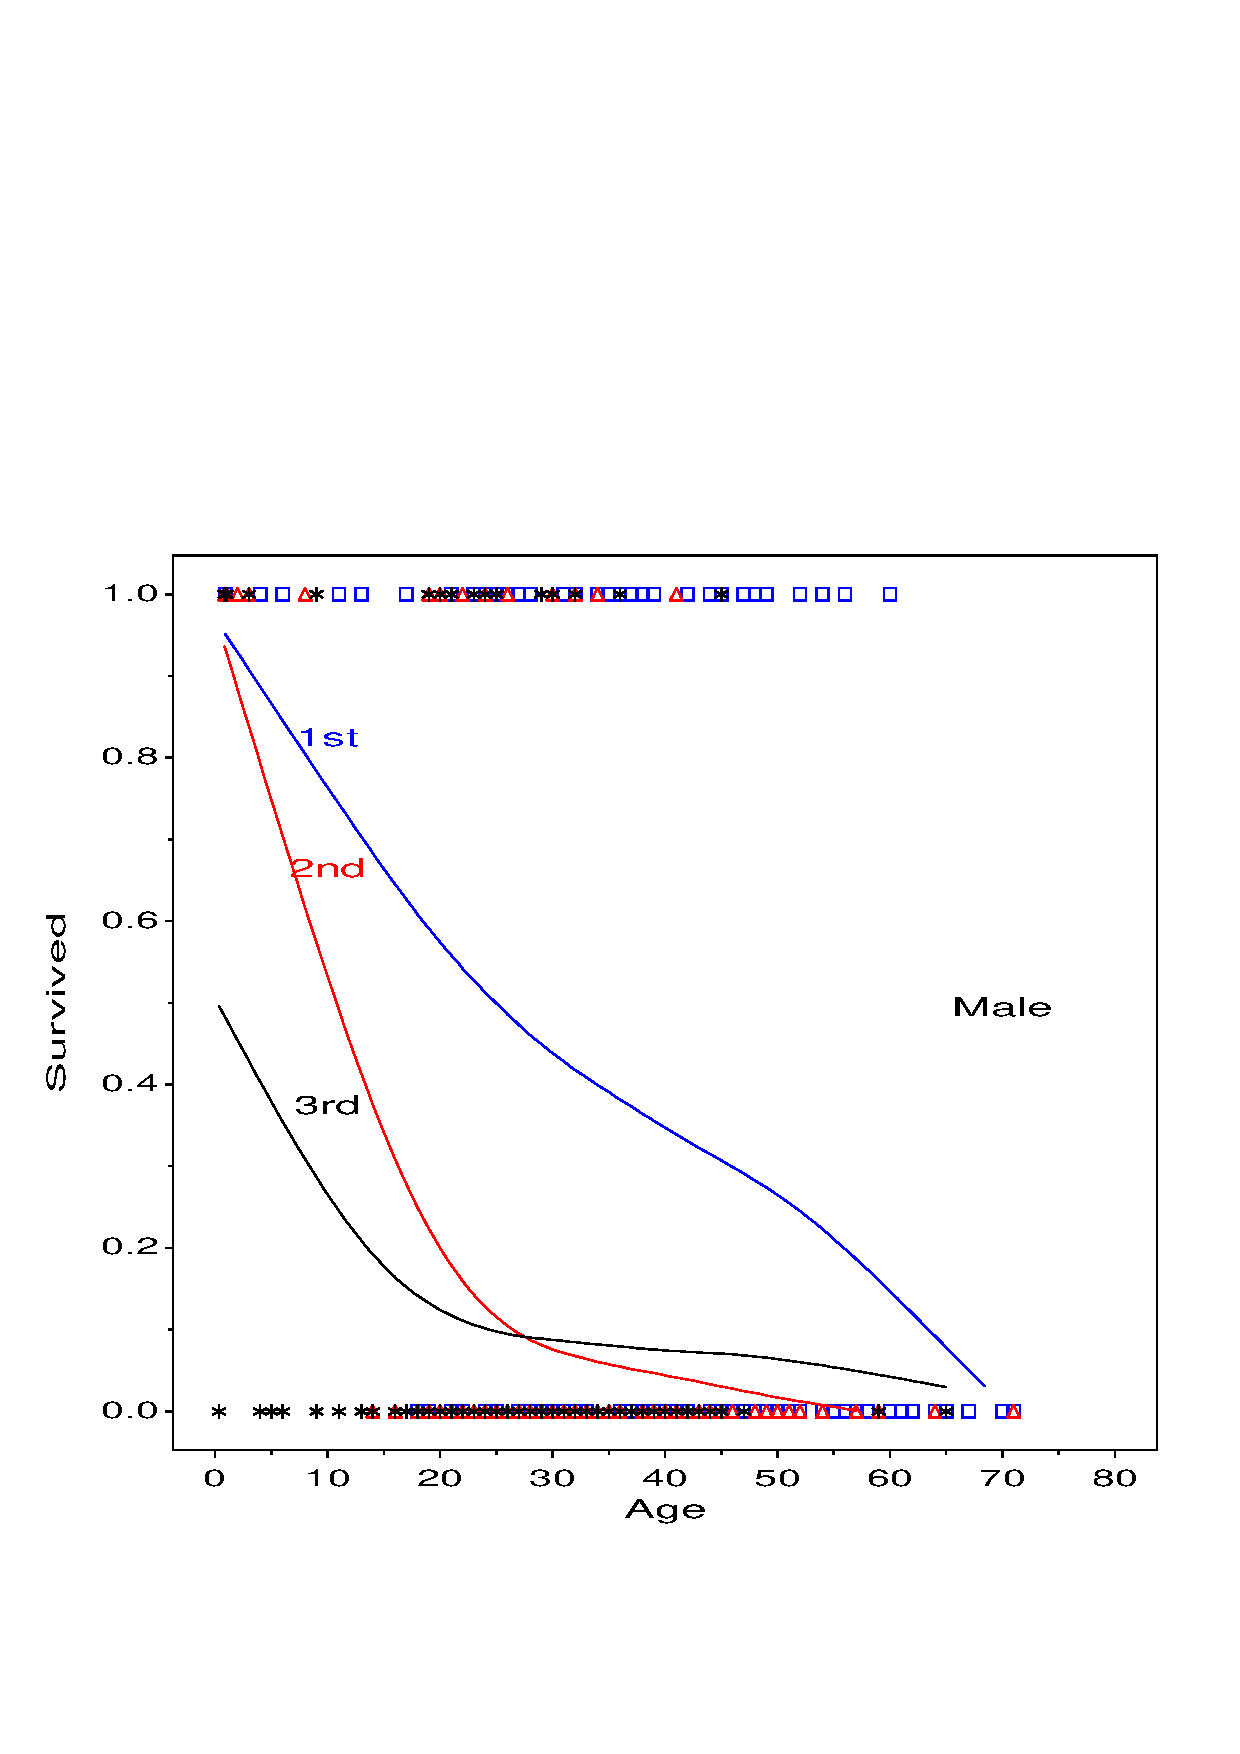
\includegraphics[width=1\linewidth]{ch6/fig/psurvive4}
 \end{minipage}
 \caption{Survival probability vs.\  age by sex--class, for passengers on the \emph{Titanic}}\label{fig:psurvive34}
\end{figure}

We can see that both assumptions are wrong by making separate graphs
for men and women.
These graphs, shown in \figref{fig:psurvive34}, are drawn
using a \stmt{BY}{GPLOT} and smoothing with the \pname{SM}
interpolation method:
\begin{listing}
goptions hby=0;
proc gplot data=titanic2 uniform;
   where (age^=.);
   plot survived * age = class /
      anno=label vm=1 hm=1 vaxis=axis1 haxis=axis2 nolegend frame;
   by sex;
    symbol1 i=sm70 v=square   h=1.9 c=blue;
    symbol2 i=sm70 v=triangle h=1.9 c=red;
    symbol3 i=sm70 v=star     h=1.9 c=black;
\end{listing}
From \figref{fig:psurvive34} it appears that survival of women actually
decreases with age in 2nd and 3rd class; the increasing overall curve
for women in \figref{fig:psurvive12} is due to the greater prevalence of
older women in 1st class, who were more likely to survive.
Among men, it now appears that survival decreases approximately linearly
in 1st class, and much more sharply in the other classes.
However, we must remember that we are just smoothing raw data here; an adequate fitted
model generally provides better smoothing
and simplification.

\end{Example}

\section{Models for quantitative predictors}\label{sec:logist-quant}
Logistic regression models may use quantitative predictors or discrete
predictors, or a mixture of both, just as in ordinary regression models.
We describe the basic theory and visualization steps for
quantitative predictors here, and extend these ideas to discrete
explanatory variables in \secref{sec:logist-qual}.

\subsection{Fitting logistic regression models}
The parameters in logistic regression models are usually estimated
by maximum likelihood.
Because the response variable, $Y$, takes on only two values, we may
take these as 
1 and 0 with probabilities
$\pi$ and $1-\pi$, respectively.  Then
the probability distribution for case $i$ can be represented
simply as
\begin{equation*}
 p ( y_i ) \equiv \Pr (Y_i = y_i) = {\pi_i}^{y_i} \: (1 - \pi_i)^{1 - y_i}
 \period
\end{equation*}
Assuming the cases are independent, the joint probability of
the $n$ observations $y_1 , y_2 , \dots , y_n$ is the
product of these probabilities over all cases,
\begin{equation*}%\label{eq:like2}
p ( y_1 , y_2 , \dots , y_n ) = \prod_{i=1}^n {\pi_i}^{y_i} \: (1 - \pi_i)^{1 - y_i}
 = \prod_{i=1}^n {\left( \frac{\pi_i}{1 - \pi_i} \right)}^{y_i} (1 - \pi_i)
 \period
\end{equation*}
Substituting for $\pi_i$ from \eqref{eq:logit3},
we can express the likelihood of the data
as a function of the model parameters,
\begin{equation}\label{eq:like3}
\mathcal{L}(\alpha, \beta) =
 \prod_{i=1}^n [ \exp( \alpha + \beta X_i ) ]^{y_i} [1 + \exp( \alpha + \beta X_i )]^{-1} \period
\end{equation}
The maximum likelihood estimates are the values of $\alpha$ and $\beta$
which maximize $ \mathcal{L}(\alpha, \beta)$,
but it is simpler to maximize $\log \mathcal{L}$,
which has its maximum at the same values.
Taking derivatives of $\log \mathcal{L}$
with respect to $\alpha$ and $\beta$
gives the estimating equations (in matrix form)
\begin{equation}\label{eq:like4}
\mat{X} \trans \vec{y} = \mat{X} \trans \hat{\vec{p}}
\comma
\end{equation}
where $ \mat{X} = [ \vec{1}, \vec{x} ]$,
and
$\hat{p_i} = \exp (\hat{\alpha} + \hat{\beta} x_i) / (1+ \exp (\hat{\alpha} + \hat{\beta} x_i) $.
This is analogous to the linear model estimating equations in
ordinary least squares regression,
$\mat{X} \trans \vec{y} = \mat{X} \trans \hat{\vec{y}}$,
where $\hat{\vec{y}} = \mat{X} \hat{\vec{\beta}}$,
and $ \hat{\vec{\beta}} =  (\mat{X} \trans \mat{X})^{-1}  \mat{X} \trans \vec{y}$.
The equations \eqref{eq:like4} have no analytic solution, but they may be solved numerically, or by iteratively
reweighted least squares.

\begin{Example}[arthrit6a]{Arthritis treatment}
It is also straight-forward to calculate the values of $\log \mathcal{L}$
in \eqref{eq:like3}
for a grid of values of $(\alpha$ , $\beta)$
and plot the log likelihood surface as a contour plot or 3D plot.
For example, the \Dstp\ below calculates the log likelihoods
over all observations in the arthritis data
for a range of $\alpha$ (\pname{b0}) and $\beta$ (\pname{b1})
determined from the parameter estimates $\pm$ two standard errors
found in \exref{ex:arthrit7}
(see \outref{out:logist1c.1}).
The contour plot, shown in \figref{fig:likefun}, has its maximum
value $\log \mathcal{L} = -54.58$ at the value
$(\hat{\alpha} , \hat{\beta}) = (-2.64, 0.05)$.  From this,
$-2 \log \mathcal{L} = 109.16$ is the value displayed for \pname{-2 LOG L} in
\outref{out:logist1c.1} for the intercept and covariates.
%% one figure
\begin{figure}[htb]
  \centering
  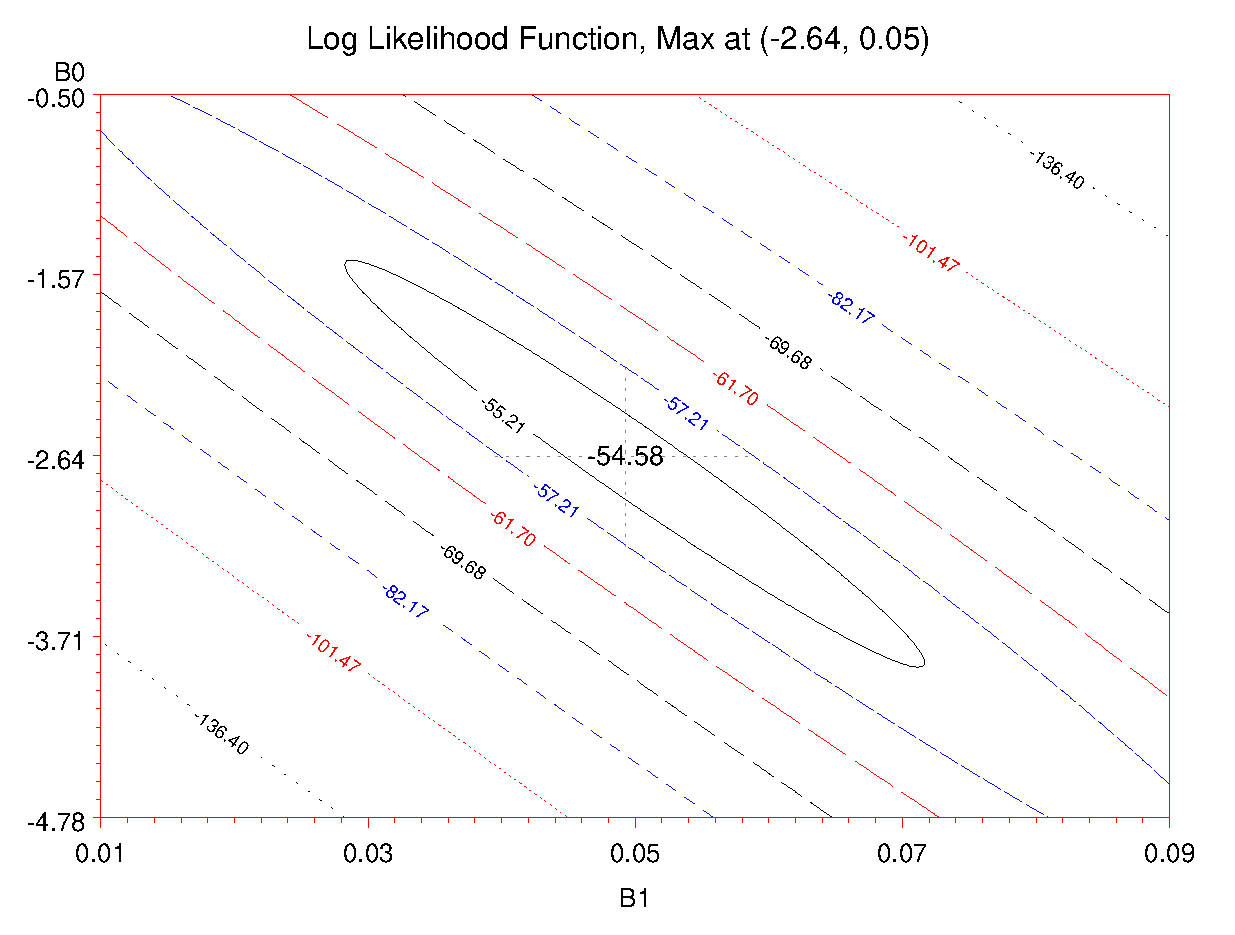
\includegraphics[clip,scale=.6]{ch6/fig/likefun}
  \caption{Contour plot of log likelihood for the Arthritis data}%
  \label{fig:likefun}
\end{figure}

\begin{listing}
data maxlike;
   keep b0 b1 loglike;
   do b0=(-2.64 - 2*1.07) to (-2.64 + 2*1.07) by (1.07/50);
      do b1=(0.05 - 2*0.02) to (0.05 + 2*0.02) by (0.02/50);
         loglike=0;
         do i=1 to n;
            set arthrit point=i nobs=n;
            phat = exp(b0+b1*age)/(1+exp(b0+b1*age));
            loglike = loglike + (better * log(phat))
                                  + ((1-better) * log(1-phat));
            end;
         output;
         end;
      end;
   stop;
\end{listing}
This contour plot of the log likelihood function shows something that
is not apparent from the usual printed output:
The contours of equal log likelihood have a pronounced negative slope,
so an increase in $\beta$ may be compensated for by a decrease in 
$\alpha$ without changing the value of $\log \mathcal{L}$ appreciably.
As well, the innermost ellipse (corresponding to the largest absolute
contour value) is relatively wide along its major axis,
reflecting the fact that the precision of these estimates is not
extremely high.   Increasing the sample size would result in tighter
estimates of the slope and intercept.
This is the visual representation of the information presented in the
covariance matrix of the parameter estimates.
\end{Example}

Logistic regression models can be fit using \PROC{LOGISTIC}, \PROC{CATMOD},
\PROC{GENMOD} and \INSIGHT.  The examples in this chapter mainly
illustrate 
the use of \PROC{LOGISTIC} because it provides the widest range of
diagnostics and other facilities for these models.
  
The input \Dset\ for \PROC{LOGISTIC} can
be in one of three forms:
\begin{description}
\item[frequency form] is used with grouped data, as in a contingency table.
For a binary response,
there are two observations per group corresponding to the levels
of the response, and a variable containing the frequency for that
group.  A \stmt{FREQ}{LOGISTIC} is used to provide the frequency
variable.

\item[events/trial form] is also used with grouped binomial data.
There is one observation per group; one variable gives the number of
events and a second variable gives the number of trials.
A \stmt{FREQ}{LOGISTIC} is also used in this situation.

\item[case form] is used when there is one observation per case.
This form  is usually required when there are quantitative predictors.
\end{description}

\subsection{Plotting predicted probabilities}\label{sec:logist-quantp}
\PROC{LOGISTIC} calculates
predicted logits \eqref{eq:logit1}
and 
predicted probabilities \eqref{eq:logit3}
for each observation.
These results may be saved in an \ODS, from which plots
can be made.  The plots, often supplemented by standard errors or
confidence bands for these predictions, provide a visual means to
interpret the prediction equations.


\begin{Example}[arthrit7]{Arthritis treatment}
This example illustrates the use of \PROC{LOGISTIC} to fit a logistic
regression model with a quantitative predictor.
It also describes the steps required
to plot the observed binary response together with fitted
probabilities and confidence intervals.
We use the arthritis treatment data, and describe how
\figref{fig:logist1c1} was produced.

The following \Dstp\ creates a \Dset\ in case form
named \pname{arthrit}.  The dichotomous response,
\pname{better} is created from the actual outcome
variable \pname{improve}, which has values 0, 1, 2
corresponding to none, some, or marked improvement.

\begin{listing}
data arthrit;
   input id treat$ sex$ age improve @@ ;
   better  = (improve > 0);            /* Dichotomous response    */
   _treat_ = (treat ='Treated') ;      /* Dummy var for treatment */
   _sex_   = (sex = 'Female');         /*           and sex       */
  cards ;
57 Treated Male   27 1   9 Placebo Male   37 0
46 Treated Male   29 0  14 Placebo Male   44 0
77 Treated Male   30 0  73 Placebo Male   50 0
  ... {\it (observations omitted)}
56 Treated Female 69 1  42 Placebo Female 66 0
43 Treated Female 70 1  15 Placebo Female 66 1
                        71 Placebo Female 68 1
                         1 Placebo Female 74 2
\end{listing}

By default, \PROC{LOGISTIC} orders the response
values in \emph{increasing} order, and sets up the model so that it is
predicting the probability of the \emph{smallest} ordered value,
Pr\{better=0\}.  This means it would be modeling the probability of No
improvement here.  
The \opt{descending}{LOGISTIC} (available with Version 6.08)
reverses this order, so that predicted results will be for
Pr\{better=1\}.

\begin{listing}
proc logistic nosimple descending;
   model  better = age / lackfit;
   output out=results p=predict l=lower u=upper;
\end{listing}
Alternatively, you can use the \opt{order}{LOGISTIC}, or
(with the default \pname{order=formatted})
you can create a user-format for the 0/1 values of the
response so that the first (smallest) formatted value corresponds
to the desired event.  In the format \pname{outcome} below, the value
``improved'' conveniently comes first alphabetically,
and so would be the predicted event.
\begin{listing}
proc format;
   value outcome 0 = 'not improved'
                 1 = 'improved';
proc logistic nosimple;
   format better outcome.;
   model  better = age / lackfit;
   output out=results p=predict l=lower u=upper;
\end{listing}
In the printed output
(\outref{out:logist1c.1}) the Response Profiles show that the response
values are ordered as desired.

\begin{Output}[htbp]
\caption{Arthritis treatment data: Logistic regression on age}\label{out:logist1c.1}
\small
\verbatiminput{ch6/out/logist1c.1}
\end{Output}
The \stmt{OUTPUT}{LOGISTIC} shown above
produces an \ODS\ (\pname{RESULTS}) containing the predicted probability of
improvement (\pname{PREDICT}) and 95\% confidence limits
(\pname{LOWER}, \pname{UPPER}) for these observations.
The first few observations from the \Dset\ \pname{RESULTS}
are shown in \outref{out:logist1c.2}.
There is one observation per case because the input data are in case form.

\begin{Output}[htb]
\caption{Arthritis treatment data: RESULTS \Dset\ (partial)}\label{out:logist1c.2}
\small
\verbatiminput{ch6/out/logist1c.2}
\end{Output}

The plot shown in \figref{fig:logist1c1} is produced
as an overlay plot by the
following \PROC{GPLOT} step.
Three \stmt{SYMBOL}{GPLOT}s are used to plot point symbols
for the observed response (\pname{BETTER}) and
interpolated lines for the
predicted probabilities of improvement and confidence limits.
The linear regression lines (and its confidence limits) in the figure are produced using
the \pname{INTERP=RLCLM} on the \pname{SYMBOL1} statement.
\begin{listing}
proc sort data=results;
   by age;
proc gplot data=results;
   plot better * age = 1
        predict * age = 2
        upper * age = 3
        lower * age = 3
        / frame overlay vaxis=axis1 vm=1 hm=1;
   axis1 label=(a=90) offset=(3) order=(0 to 1 by .2);
   symbol1 v=dot h=1.4 i=rlclm l=2 c=green ci=red;
   symbol2 v=none   i=join l=1  w=3 c=blue;
   symbol3 v=none   i=join l=20 w=3 c=blue;
   label better='Probability (Improved)';
   format better 4.1;
   title2  c=red 'Linear' c=black ' and ' c=blue 'Logit '
           c=black 'Regressions on Age';
run;
\end{listing}
The model fitting tests in \outref{out:logist1c.1}
(``Chi-Square for Covariates'' and the Wald test for \texttt{age})
test whether
age adds significantly to predicting outcome.
This is a different question than whether the model is adequate---usually
provided by a \glossterm{lack of fit test},
comparing the given model to the saturated model.
However,
with binary data in case form, the usual lack of fit tests
do not apply.
The \opt{lackfit}{LOGISTIC} on the \stmt{MODEL}{LOGISTIC}
requests a lack-of-fit test
\ix{lack-of-fit test}
proposed by \citet{HosmerLemeshow:89}.  This test divides subjects
into tenths based on their ordered predicted probabilities. It then computes a
\(\chi^2\) from the observed and expected frequencies in these 10 groups. 
The results from this test,
shown in \outref{out:logist1c.3} do not reject the fit of the simple
one-variable model;  however, the relatively small $p$-value suggests that the model
might be improved.
\begin{Output}[htbp]
\caption{Arthritis treatment data: Goodness-of-fit test}\label{out:logist1c.3}
\small
\verbatiminput{ch6/out/logist1c.3}
\end{Output}
\end{Example}

%\subsubsection{The \emph{Challenger} disaster}
\begin{Example}[nasa]{Challenger disaster}
\ixd{Challenger disaster|(}
\begin{changebar}
The space shuttle \emph{Challenger} exploded 73 seconds after take-off on
\end{changebar} 
January 28, 1986.
Subsequent investigation determined that the cause was failure of the O-ring
seals used to isolate the fuel supply from burning gases.
The story behind the \emph{Challenger} disaster is perhaps the most poignant
missed opportunity in the history of statistical graphics.
It may be heartbreaking to find out that some important information
was there, but the graph maker missed it.

Engineers from Morton Thiokol, manufacturers of the rocket motors,
had been worried about the effects of unseasonably cold weather
on the O-ring seals and recommended aborting the flight.
NASA staff analysed the data on the relation between ambient temperature
and the number of O-ring failures (out of 6), but they had excluded observations
where no O-rings failed,
believing that they were uninformative.
Unfortunately, those observations had occurred when the launch temperature
was relatively warm (\degree{65-80}F.) and were indeed informative.
The coldest temperature at any previous launch was \degree{53};  when \emph{Challenger} was launched on January 28,
the temperature was a frigid \degree{31}.

The data relating O-ring failures to temperature were depicted as in
\figref{fig:nasa0}, our candidate for the most misleading graph of history.
Examination of this graph seemed to indicate that there was no relation
between ambient temperature and failure.  Thus, the decision to launch
the \emph{Challenger} was made, in spite of the initial concerns
of the Morton Thiokol engineers.
\begin{figure}[htb]
  \centering
  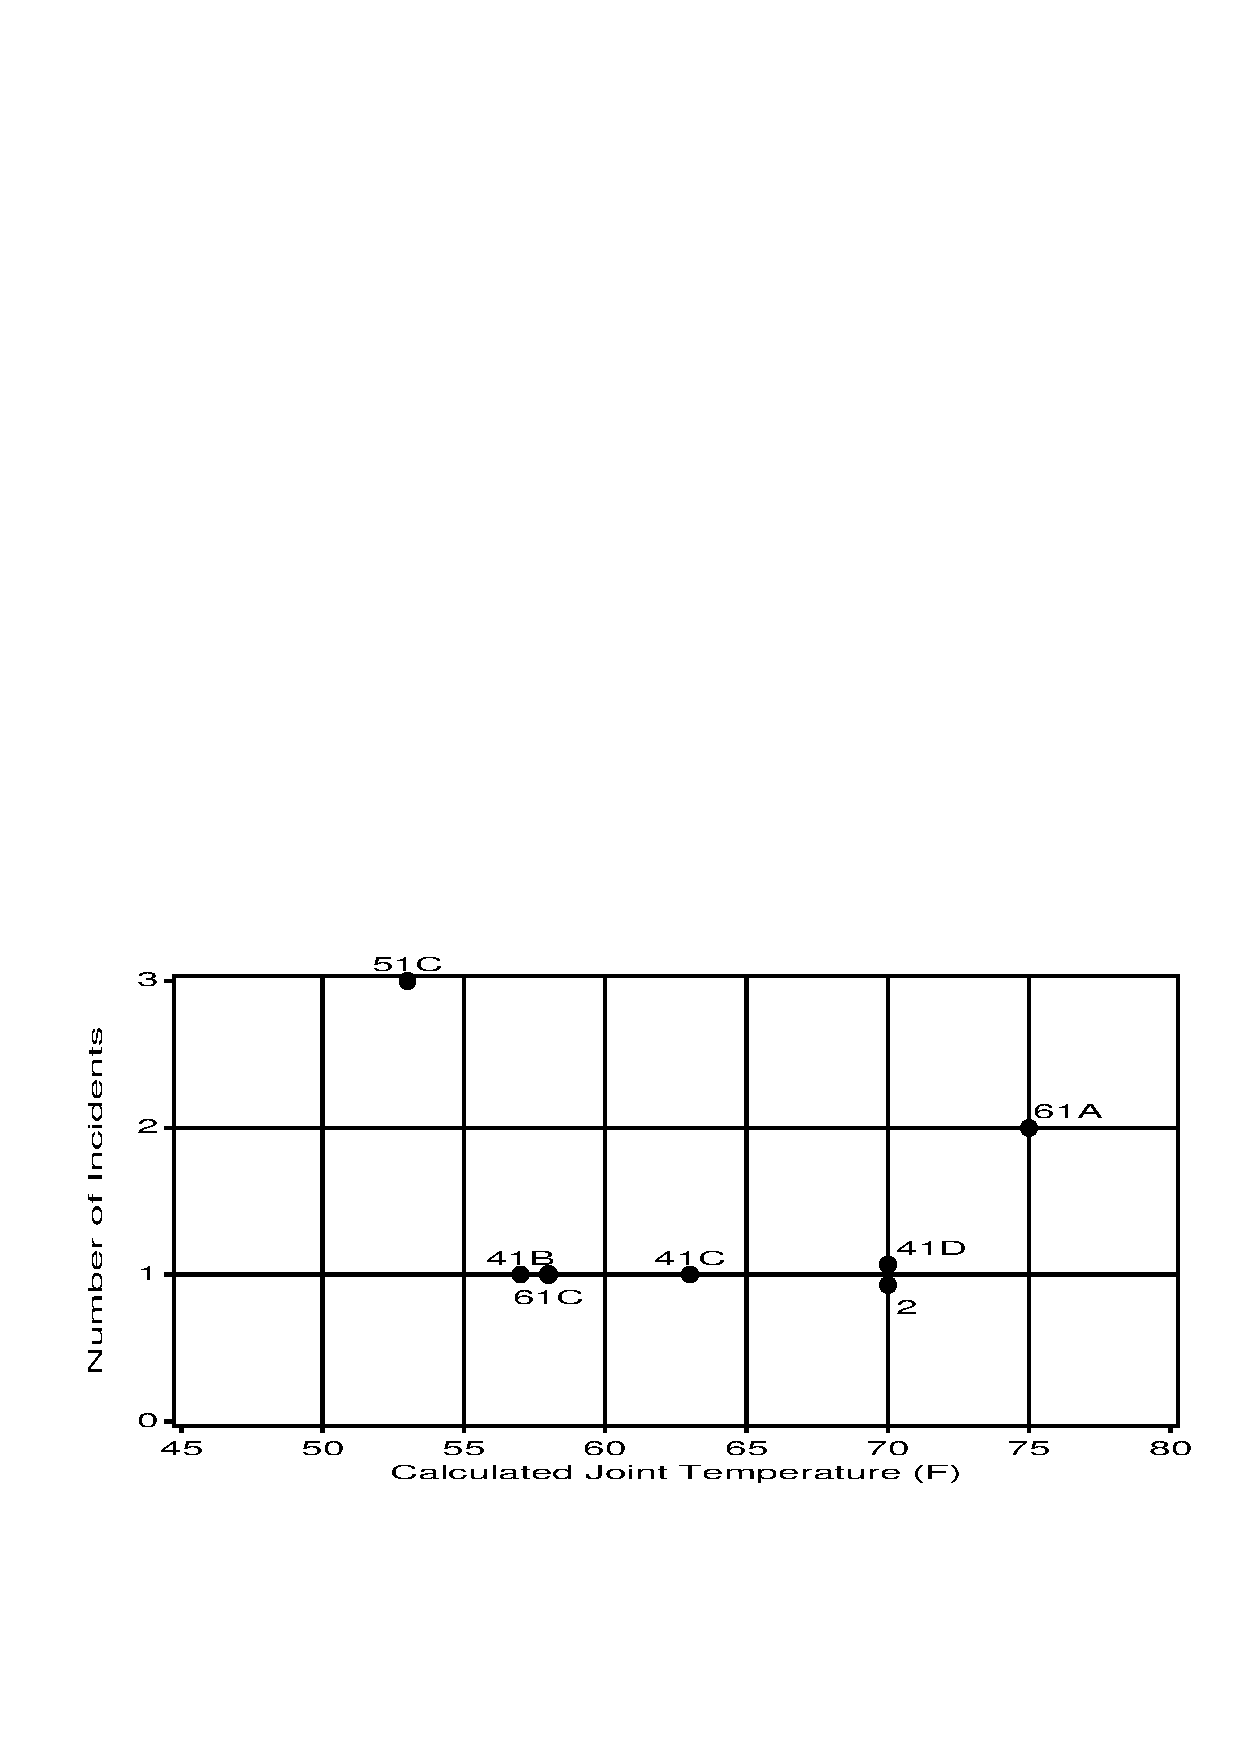
\includegraphics[width=\textwidth,clip]{ch6/fig/nasa0}
  \caption{NASA Space Shuttle pre-launch graph}\label{fig:nasa0}
\end{figure}

These data have been analyzed extensively
\citep{Dalal-etal:89,Lavine:91}.
\citet{Tufte:97} gives a thorough and convincing
visual analysis of the evidence available prior to the launch.
The main goal here is to
illustrate predictions from the model for the \emph{Challenger} launch
and graphical display.
But, what if the engineers had simply made a better graph?
At the least, that would entail
\begin{seriate}
\item drawing a smoothed curve to fit the points (to show the trend)
\item removing the background grid lines (which obscure the data).
\end{seriate}
\figref{fig:nasa02} 
shows a revised version of the same 
graph, which should have caused any engineer to conclude that
either 
\begin{seriate}
\item the data were wrong, or
\item there were excessive risks
associated with both high and low temperatures.
\end{seriate}
But it is well-known
that brittleness of the rubber used in the O-rings is inversely
proportional to $(\texttt{temp})^3$, so prudent interest might have focussed
on the first possibility.

\begin{figure}[htb]
  \centering
  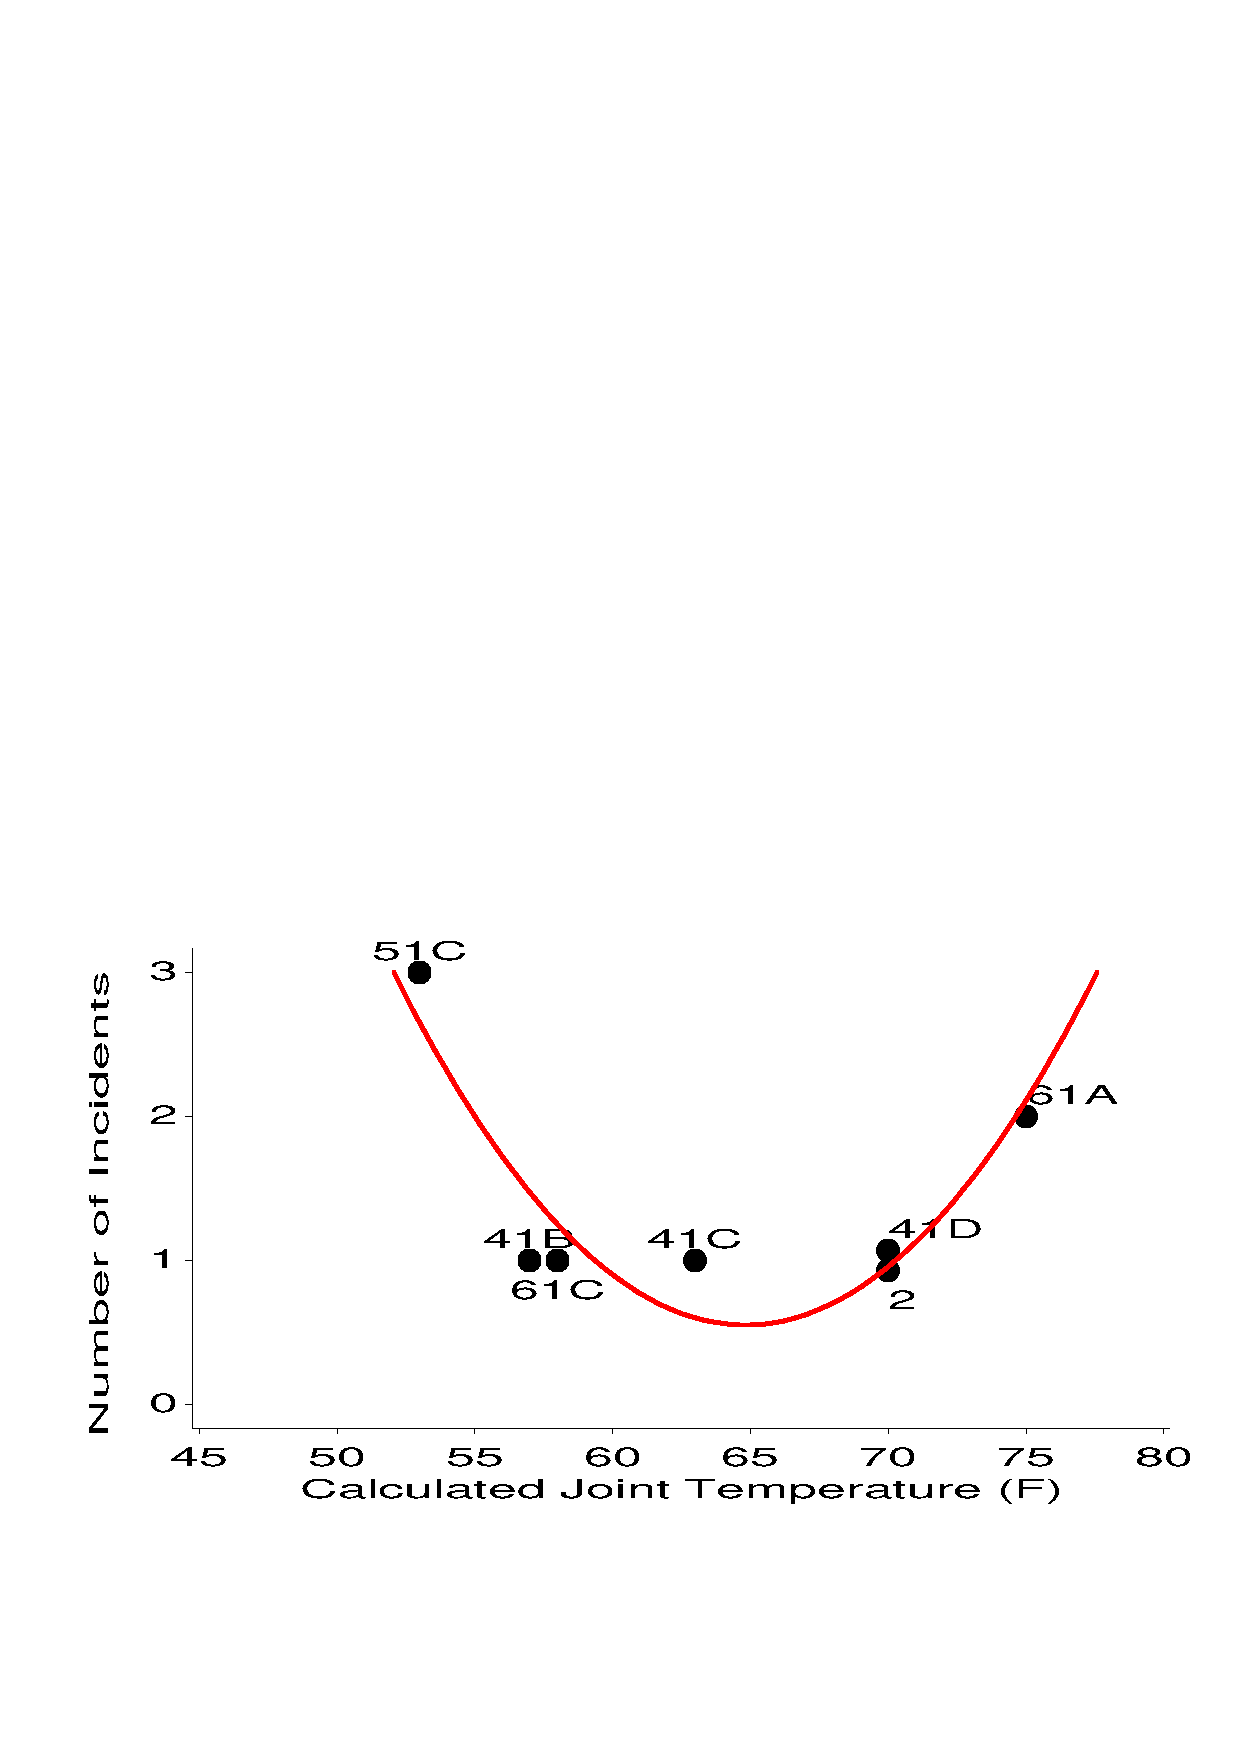
\includegraphics[clip,width=\textwidth]{ch6/fig/nasa02}
  \caption{NASA Space Shuttle pre-launch graph, revised}\label{fig:nasa02}
\end{figure}

We return to the problem of predicting the likelihood of failures at
low temperatures.
The \Dstp{} below reads the data on the number of O-ring failures
and temperature for the 23 flights for which information was available
before the \emph{Challenger} launch.  A more detailed \Dset,
from \citet{Dalal-etal:89} and \citet{Tufte:97} is given in \datref{dat:orings}.

\begin{listing}
title 'NASA Space Shuttle O-Ring Failures';
data nasa;
   input failures temp @@;
   orings = 6;
   label failures = 'Number of O-ring failures'
      temp = 'Temperature (deg F)';
   datalines;
   2  53    1  57    1  58     1  63
   0  66    0  67    0  67     0  67
   0  68    0  69    0  70     0  70
   1  70    1  70    0  72     0  73
   0  75    2  75    0  76     0  76
   0  78    0  79    0  80
;
\end{listing}
To obtain predicted probabilities for observations not in the original sample,
create an additional \Dset\ which contains values for the independent
variables in the extrapolation sample, and join these observations to the
actual \Dset.  The response variable (\texttt{failures}) will be missing
for the extrapolation sample.

\begin{listing}
*-- Obtain predicted values for 30-80 degrees;
data temp;
   input temp @@;
datalines;
31 30 35 40 45 50 55 60 65 70 75 80
;
data nasa2;
   set nasa temp;
\end{listing}
In the \PROC{LOGISTIC} step, we use the \boldital{events/trials} syntax
to indicate the number of failures and number of trials.
(This does assume that O-rings on the same flight fail independently.)
The observations in the extrapolation sample are not used in fitting
the model, yet the procedure produces predicted probabilities and
logits (as long as the independent variable(s) are non-missing).

\begin{listing}
proc logistic data=nasa2 nosimple;
   model failures/orings = temp ;
   output out=results p=predict l=lower u=upper;
proc print;
\end{listing}
The printed output, shown in \outref{out:nasa.1} indicates that the
12 new observations were not used in the analysis.
The odds ratio, 0.891, is interpreted to mean that each increase of
\degree{1} in temperature decreases the odds of a failure by 11\%!

\begin{Output}[htbp]
\caption{Logistic regression for NASA O-ring data}\label{out:nasa.1}
\small
\verbatiminput{ch6/out/nasa.1}
\end{Output}

The \ODS\ \pname{results} contains the predicted probability
of a failure of a single O-ring
at each temperature and upper and lower confidence 95\% limits
for this probability.  We can plot the predicted and observed values
as shown below.  A vertical reference line at \degree{31} is used
to highlight the conditions at the \emph{Challenger} launch.
\begin{listing}
proc sort data=results;
   by predict;
data results;
   set results;
   obs = failures / orings;

proc gplot data=results;
   plot (obs predict lower upper) * temp /
      href=31 lhref=33
      overlay frame vaxis=axis1 vminor=1;
   symbol1 v=dot i=none c=blue h=2;
   symbol2 v=none i=spline c=black w=5;
   symbol3 v=none i=spline c=red l=33 r=2 w=3;
   axis1 label=(a=90 'Estimated Failure probability') offset=(3);
\end{listing}

The graph is shown in \figref{fig:nasa}.  There's hardly any data
at low temperatures and the width of the confidence band provides
an important visual cue to this uncertainty. Nevertheless,
the predicted probability of failure per O-ring is uncomfortably
 high at \emph{all} temperatures below the range of data from
previous flights.  Would you take a ride on \emph{Challenger} when
the weather is cold?

\begin{figure}[htb]
  \centering
  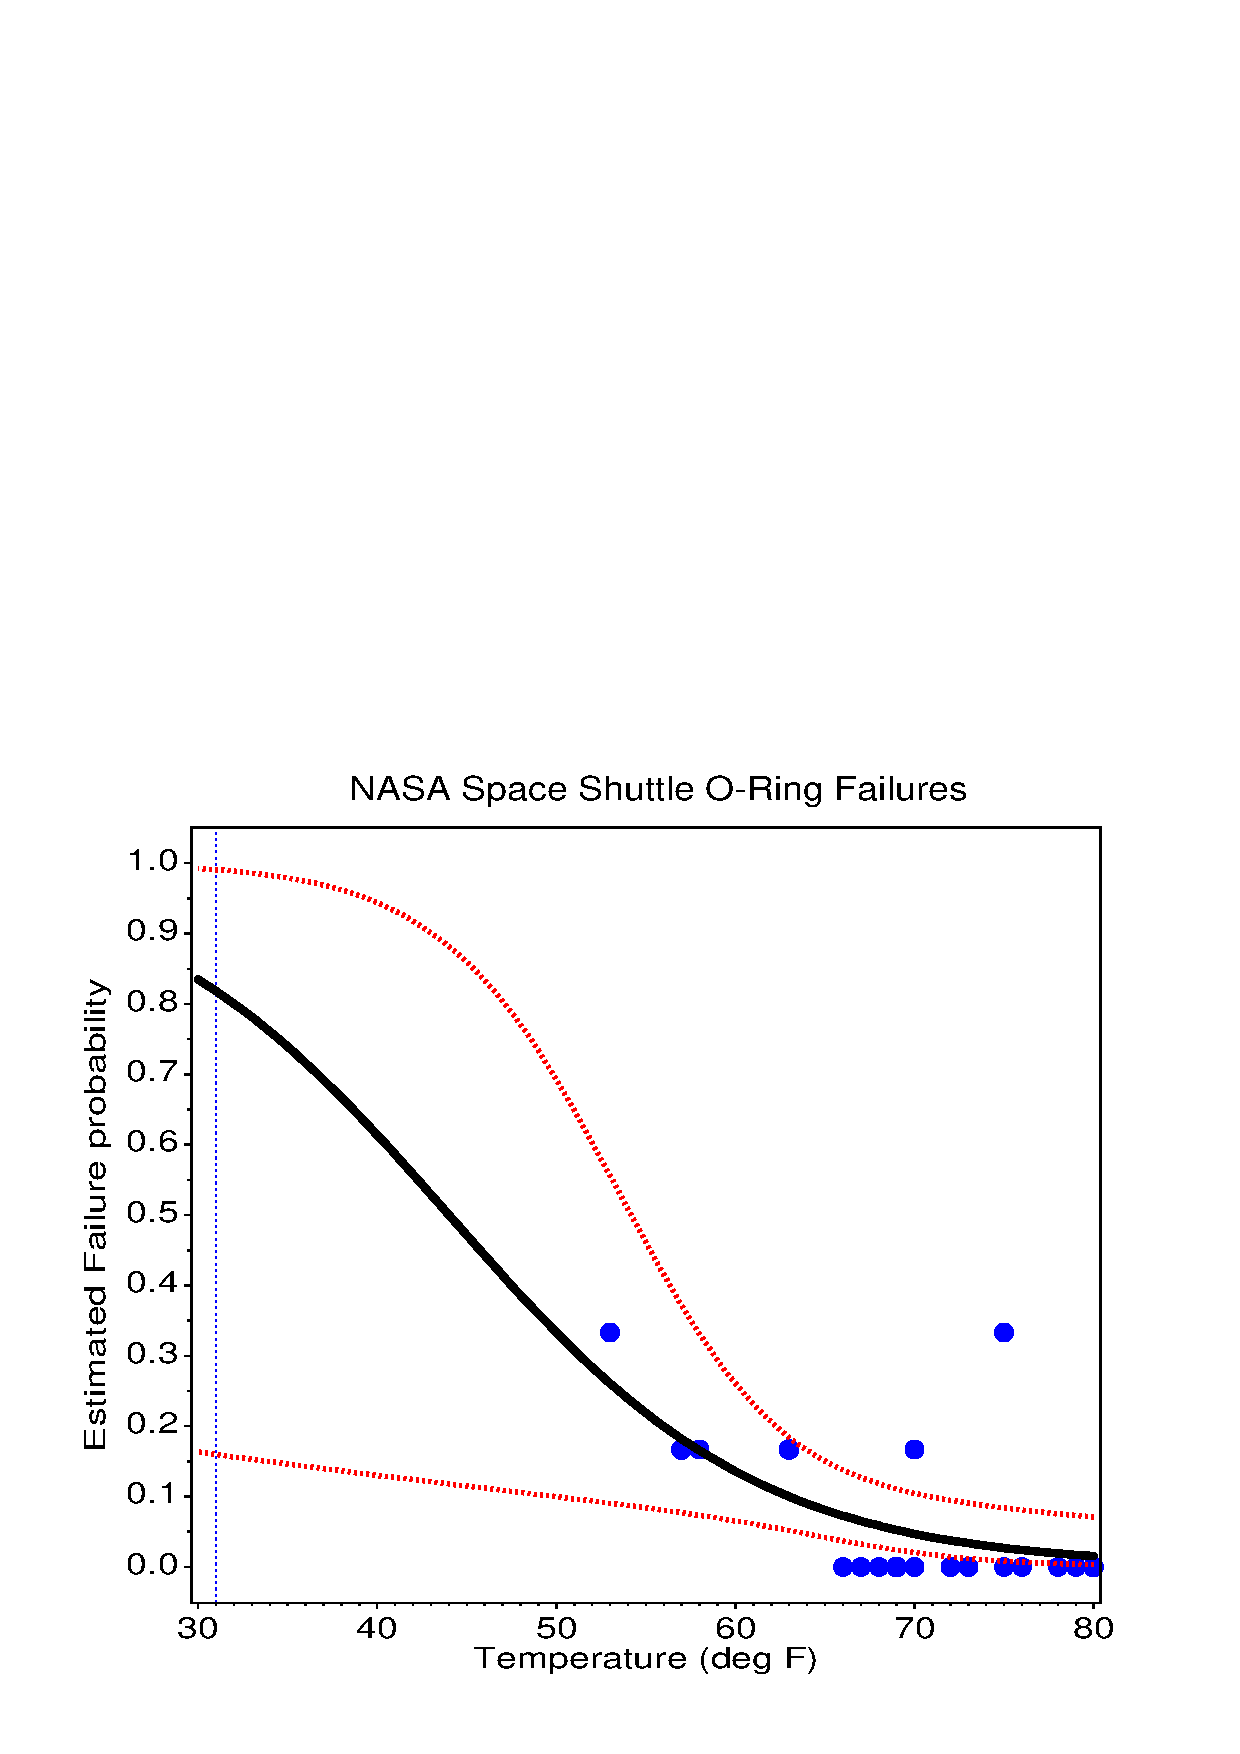
\includegraphics[scale=.75]{ch6/fig/nasa}
  \caption{NASA Space Shuttle O-ring Failure, Observed and Predicted probabilities}\label{fig:nasa}
\end{figure}
\ixd{Challenger disaster|)}
\end{Example}



\section{Logit models for qualitative predictors}\label{sec:logist-qual}

Logistic regression can be generalized to include discrete
explanatory variables, and such models are often called
\glossterm{logit models}.
The main differences (using \PROC{LOGISTIC}) are:

\begin{itemize*}
\item the data are often entered in frequency form, with one observation
       per ``group'', defined by the value(s) of the discrete predictors.
		 With quantitative predictors, the data \emph{must} be entered in
		 \IX{case form}.
\item the discrete predictors must be represented by dummy (0/1) variables
for \PROC{LOGISTIC},
so explanatory variables often need to be recoded.%
\footnote{The \proc{GENMOD} provides a \stmt{CLASS}{GENMOD}, so no
recoding is necessary. The \macro{DUMMY} (\macref{mac:dummy}) may be used
to create the dummy variables for \PROC{LOGISTIC}.}
\item the statistics for goodness-of-fit are computed differently.

\item the \ODS\ used for plotting contains one observation
 per group when the data are in frequency form.
\end{itemize*}

When \emph{all} predictors are discrete, the data actually comprise
a contingency table, and there is a close connection between logit
models and \loglin\ models discussed in \chref{ch:loglin},
so that the methods of that chapter may also be used to analyse the data
presented here. 

Consider the data below, which represents the contingency table for
the arthritis data (\exref{ex:arthrit1})
classified by sex and treatment, ignoring the age variable for the moment.  For each group, the observed probabilities and logits
may be found, as displayed in \tabref{tab:arthlogit3}.
\begin{verbatim}
                        Improvement
  Sex   Treatment    None    Some/Marked     Total

   F     Active        6         21            27
   F     Placebo      19         13            32

   M     Active        7          7            14
   M     Placebo      10          1            11
\end{verbatim}
\begin{table}[htb]
 \caption{Arthritis data, by sex and treatment}\label{tab:arthlogit3}
 \begin{center}
 \begin{tabular}{|ll|rrrrr|}
 \hline
      &           & Number &       & Observed &   Odds & Observed \\
  Sex & Treatment & Better & Total & Pr\{better\} & Better & Logit \\ 
   \hline 
  Female & Active & 21 & 27 & 0.7778 & 3.50 & 1.2529 \\ 
  Female & Placebo & 13 & 32 & 0.4062 & 0.68 & -0.3797 \\ 
  Male & Active & 7 & 14 & 0.5000 & 1.00 & 0.0000 \\ 
  Male & Placebo & 1 & 11 & 0.0909 & 0.10 & -2.3026 \\ 
 \hline
 \end{tabular}
 \end{center}
\end{table}


A simple model might assume additive (``main'') effects
for sex and treatment on the log odds of improvement,
of the same form as model \eqref{eq:logit1}.
\begin{equation} \label{eq:logst}
  \logit \,  ( \pi_{ij} ) = \alpha   +
  \beta _1 \,  x_1  +
  \beta _2 \,  x_2
  \period
\end{equation}
In this model,
\begin{itemize}

\item \(x_1\) and \(x_2\) are dummy (0/1) variables representing sex and
       treatment, respectively.  They are defined as 
\begin{equation*}
 x_1 = \left\{
    \begin{array}{ll}
    0  & \mbox{ if male} \\
    1  & \mbox{ if female}
    \end{array}
    \right.
 \qquad\qquad
 x_2 = \left\{
    \begin{array}{ll}
    0  & \mbox{ if placebo} \\
    1  & \mbox{ if active}
    \end{array}
    \right.
\end{equation*}
\item \(\alpha\) is the log odds of improvement for the baseline group
with $x_1=0$ and $x_2=0$---males receiving
the placebo.

\item \(\beta_1\) is the increment in log odds for being female
as opposed to male.
Therefore, \(e^{ \beta_1 }\) gives the odds of improvement
for females relative to males.

\item \(\beta_2\) is the increment in log odds for being in the
active treatment group.  \(e^{ \beta_2 }\) gives the odds of
improvement for the active treatment group relative to
placebo.

\end{itemize}

Thus, the parameters defined here are \emph{incremental effects}.  The
intercept corresponds to a baseline group (males given the placebo);
the other parameters are incremental effects for the other groups
compared to the baseline group.
Thus, when \(\alpha\), \(\beta _1\), and \(\beta _2\) have
been estimated, the fitted logits and predicted odds are:

\begin{center}
\vspace{1ex}
{\renewcommand{\arraystretch}{1.2}
\begin{tabular}{|ll|cc|}
\hline
Sex  &  Treatment & Logit & Odds Improved  \\[.5ex] \hline

Female & Active & \(\alpha + \beta_1 + \beta_2\) & \(e^{\alpha + \beta_1 + \beta_2}\)  \\
Female & Placebo & \(\alpha + \beta_1 \) & \(e^{\alpha + \beta_1 }\) \\
Male   & Active  & \(\alpha + \beta_2 \) & \(e^{\alpha + \beta_2 }\) \\
Male  & Placebo  & \(\alpha \) & \(e^{\alpha}\) \\ \hline
\end{tabular}
}
\end{center}

In general, there may be any number of explanatory variables, as in multiple
regression.  A discrete predictor with $c$ categories may be represented
by  $c-1$ dummy variables.  Interactions between predictors may be included
in the model by defining interaction variables as products of the main effect variables, as with \PROC{REG}.
For example, the interaction of sex and treatment could be included in the
model \eqref{eq:logst} by adding a term
$\beta_3 x_3$, where $x_3 = x_1 \times x_2$.%
\footnote{In the current example, this would give a saturated model,  which would
necessarily fit perfectly.
We usually try to obtain the simplest model with an adequate fit.}

\begin{Example}[arthrit8]{Arthritis treatment}
The following \Dstp\ creates a \Dset\ in frequency form
named \pname{ arthrit}.  The dummy variables \verb|_SEX_| and \verb|_TREAT_|
corresponding to \(x_1\) and \(x_2\) are created with logical assignment
statements, 
as is the
dichotomous response variable, \pname{ better}.

The first logistic regression model includes effects for sex and
treatment, specified by the dummy variables in the \stmt{MODEL}{LOGISTIC}.
Again,
the \opt{descending}{LOGISTIC} is used
so that predicted results will be for
Pr\{better=1\}.

\begin{listing}
data arthrits;
   input sex$ trtment$ improve$ count;
   _treat_ = (trtment='Active');
   _sex_   = (sex='F');
   better  = (improve='some');
datalines;
F Active  none   6
M Active  none   7
F Active  some  21
M Active  some   7
F Placebo none  19
M Placebo none  10
F Placebo some  13
M Placebo some   1
;
proc logistic data=arthrits descending;
   freq count;
   model better = _sex_ _treat_ / scale=none aggregate;
\end{listing}
The options \pname{scale=none aggregate} provide goodness of fit tests%
\glosstex{goodness-of-fit}
for the model.  The goodness of fit tests are based on the difference
between the actual model fitted and the saturated model (containing
an interaction of sex and treatment in this example), which would fit
perfectly.  The results shown in \outref{out:glogist0.1} are produced.
\begin{Output}[htb]
\caption{Arthritis treatment data: Overall tests}\label{out:glogist0.1}
\small
\verbatiminput{ch6/out/glogist0.1}
\end{Output}
The Chi-square tests for BETA=0 in \outref{out:glogist0.1} test the joint effect of sex
and treatment.  Individual effects in the model are tested by Wald
\ix{Wald test}
\(\chi^2\)s, the squared ratio of each parameter divided by its
standard error.  These tests, in \outref{out:glogist0.2}, indicate that both sex and
treatment effects are highly significant.

\begin{Output}[htb]
\caption{Arthritis treatment data: Parameter estimates}\label{out:glogist0.2}
\small
\verbatiminput{ch6/out/glogist0.2}
\end{Output}
The fitted model,

\begin{equation} \label{eq:fitmod}
  \logit ( \pi_{ij} ) = -1.90  +  1.47 \, \mbox{sex}
  +  1.78 \, \mbox{treat}
\end{equation}
is most easily interpreted by considering the odds ratios
corresponding to the parameters:

\begin{itemize}

\item 1.47 is the increment to log odds of a better outcome for
       females; the \IX{odds ratio} \(e^{1.47} = 4.34\) indicates that
       females are 4.3 times as likely to achieve a better outcome
       than males.

\item 1.78 is the increment to log odds for the treatment group; the
       odds ratio \(e^{1.78} = 5.94\) indicates that the treated
       group is nearly 6 times as likely to achieve a better outcome
       than the placebo group.

\end{itemize}
\end{Example}

\subsection{Plotting results from \PROC{LOGISTIC}}\label{sec:qual-plots}
As we saw in \secref{sec:logist-quantp}, you can save predicted probabilities and fitted logits in an
\ODS\ which may be used for plotting and visualizing the results.

\begin{Example}[arthrit9]{Arthritis treatment}
Adding an \stmt{OUTPUT}{LOGISTIC} to the \PROC{LOGISTIC} step produces a \Dset\ containing estimated
logit values for each group, and corresponding predicted
probabilities of improvement and confidence limits (\pname{UPPER}, \pname{LOWER}) for these probabilities.

\begin{listing}
proc logistic data=arthrits;
   freq count;
   format better outcome.;
   model better = _sex_ _treat_;
   \textbf{output out=results p=predict l=lower u=upper xbeta=logit;}
proc print data=results;
   id sex trtment; var improve count predict lower upper logit;
   format predict lower upper logit 7.3;
\end{listing}
The \ODS\ \pname{RESULTS} is shown in \outref{out:glogist0.3}.
There are two observations for each group (for none and some
improvement).  The \pname{PREDICT} variable gives the predicted
probability of an improved outcome according to model \eqref{eq:fitmod}, using the
inverse transformation \eqref{eq:logit3} of logit to probability.
Note that the fitted statistics are the same for both observations
corresponding to each sex-treatment combination.
\begin{Output}[htb]
\caption{Arthritis treatment data: \pname{RESULTS} \Dset}\label{out:glogist0.3}
\small
\verbatiminput{ch6/out/glogist0.3}
\end{Output}

To plot the predicted probabilities of improvement and confidence
limits from the \pname{RESULTS} \Dset, we select the observations
for \pname{improve='some'}.  A plot can be done as a bar chart with \PROC{GCHART},
or as a line graph with \PROC{GPLOT}.  Confidence limits can be
added to either with the SAS/GRAPH Annotate facility.  The statements
below show how a grouped horizontal bar chart (see \figref{fig:glogist0})
is constructed.
\begin{listing}
data results;
   set results;
   if improve='some';
   label predict='Prob. Improved';
data limits;
   set results;
   xsys='2'; ysys='2';
   midpoint=trtment;
   group=sex; when='A'; position='+';
   x = lower;  function='MOVE   '; output;
   text='|';   function='LABEL  '; output;
   x = upper;  function='DRAW   '; output;
   text='|';   function='LABEL  '; output;

proc gchart data=results;
   hbar trtment / sumvar=predict group=sex gspace=3
                  patternid=midpoint
                  anno=limits
                  raxis=axis1
                  maxis=axis2
                  gaxis=axis3;
   axis1 order=(0 to 1 by .2) minor=none
         label=(h=1.5) value=(h=1.3);
   axis2 label=(h=1.3 'Treat') value=(h=1.1);
   axis3 label=(h=1.3) value=(h=1.2);
   pattern1 v=solid c=cyan;
   pattern2 v=solid c=rose;
\end{listing}
\begin{figure}[!htb]
  \centering
  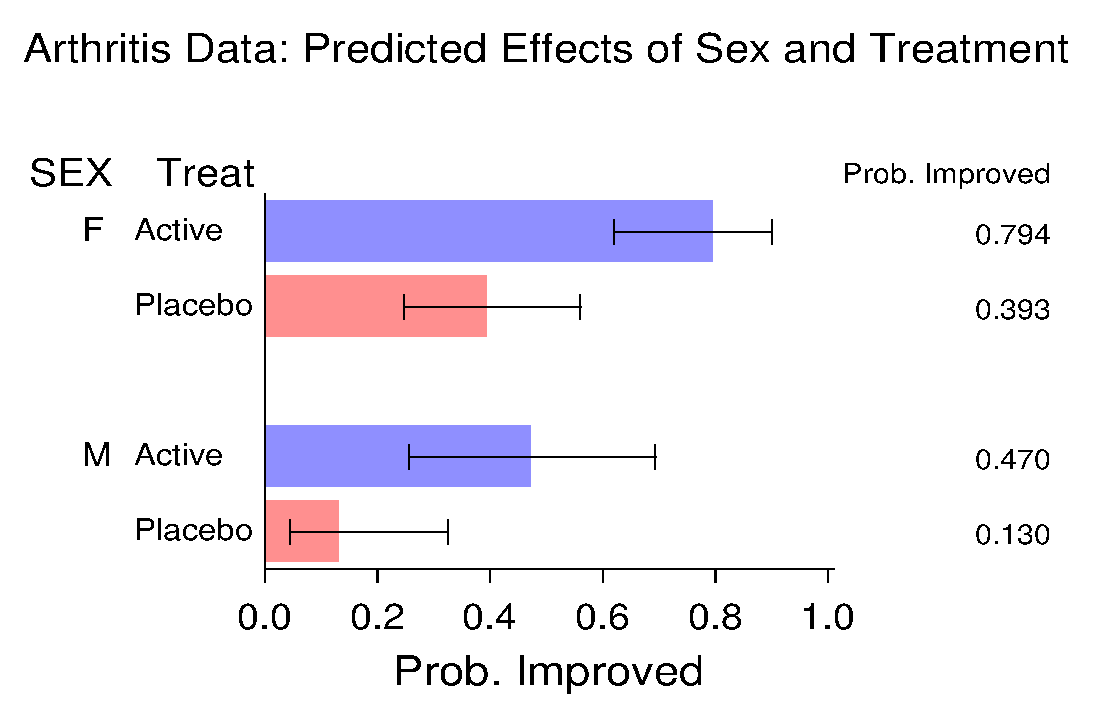
\includegraphics[scale=.7,clip]{ch6/fig/glogist0}
  \caption{Predicted probabilities of improvement}\label{fig:glogist0}
\end{figure}

Alternatively, you may prefer a line graph to a bar chart.
\figref{fig:glogist11} shows one example, with separate lines
for the two treatment groups.
The observed probabilities of improvement are shown by dots;
these values were calculated from the \pname{COUNT} variable
in the \pname{RESULTS} \Dset.
The plotting steps are not shown here to conserve space.
\begin{figure}[!htb]
  \centering
  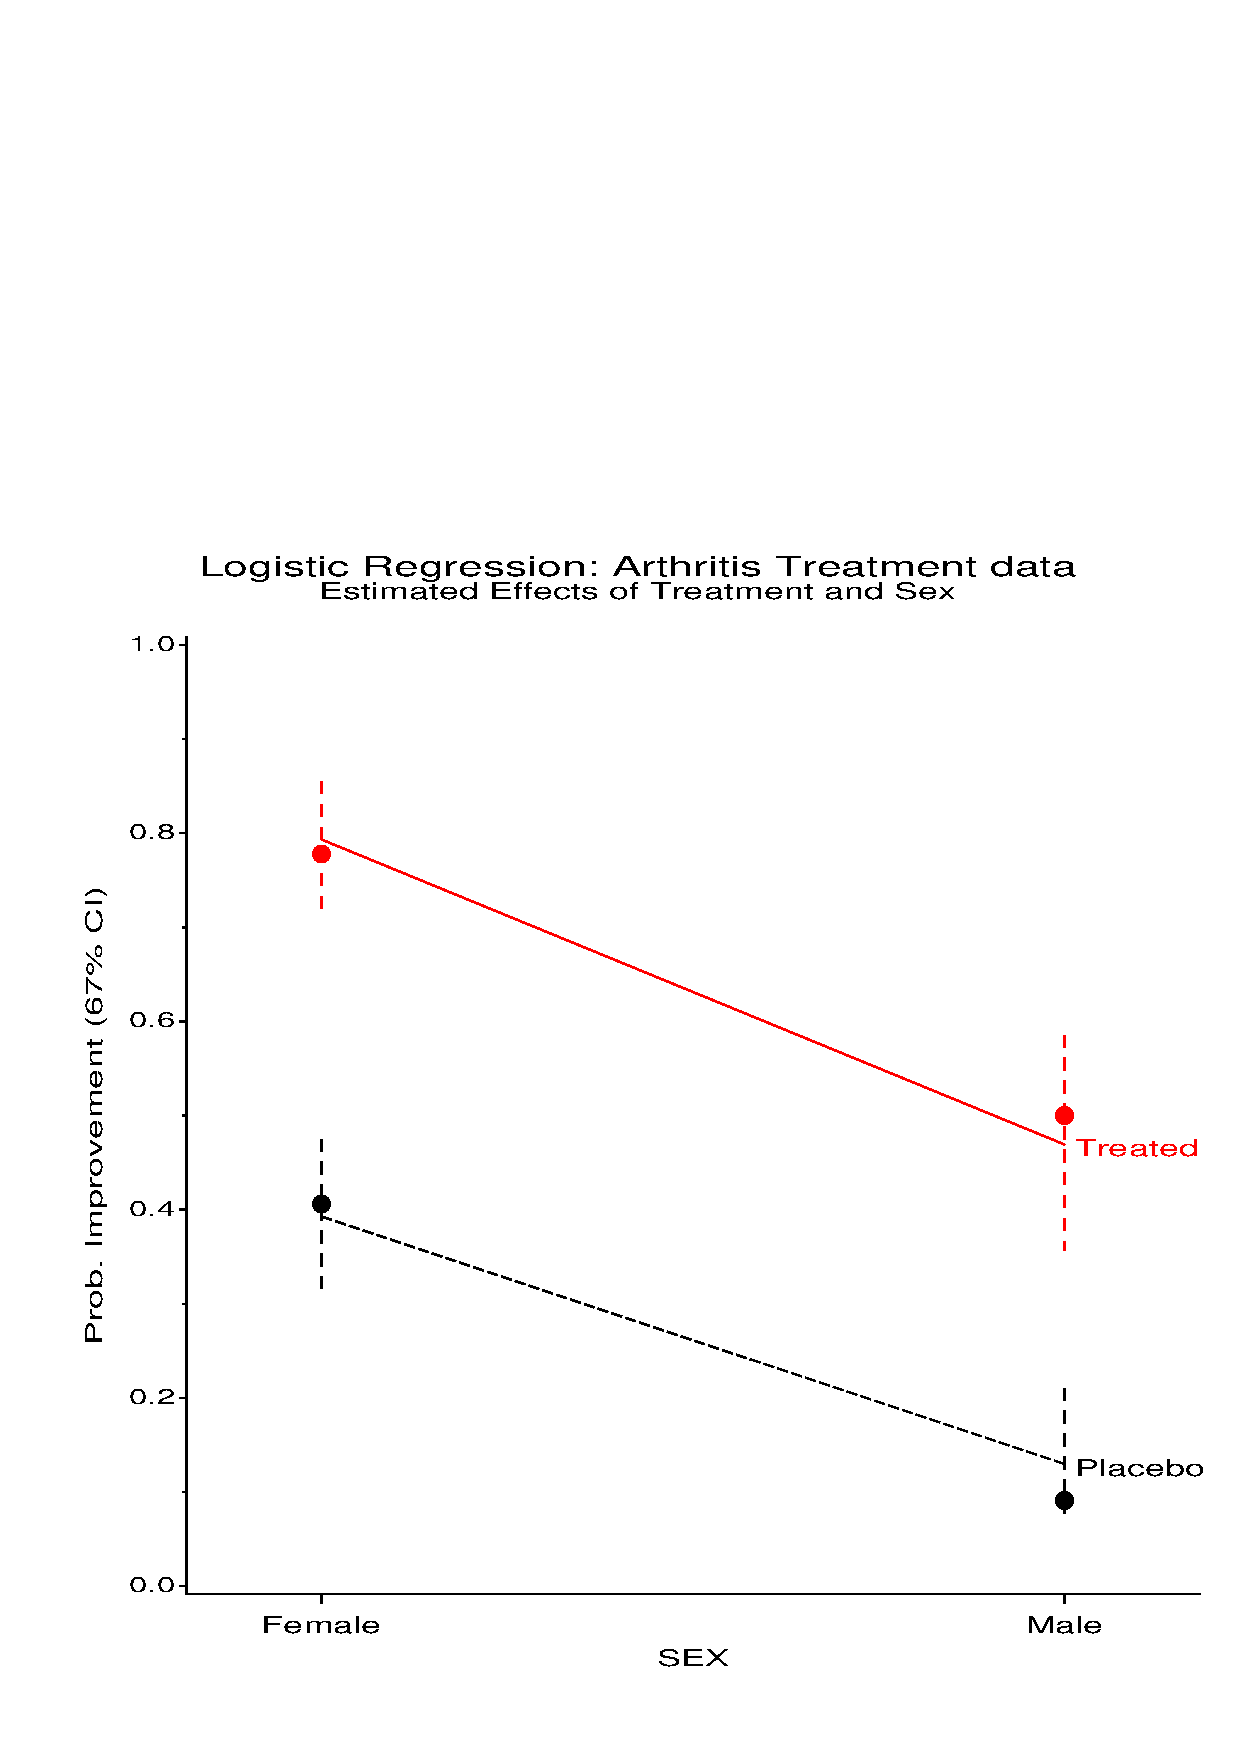
\includegraphics[scale=.7]{ch6/fig/glogist11}
  \caption{Line graph of observed and predicted probabilities}\label{fig:glogist11}
\end{figure}
\end{Example}
 

\section{Multiple logistic regression models}\label{sec:logist-mult}
The logistic regression model can be generalized to include an
arbitrary number of explanatory variables,
\begin{eqnarray}
  \logit ( \pi_{i})
   &=& \alpha + \vec{x}_{i}\trans \,  \vec{\beta} \\ \label{eq:logisr}
   &=& \alpha + \beta_1 x_{i1} + \beta_2 x_{i2} + \cdots + \beta_p x_{ip}
   \nonumber
\end{eqnarray}
The $x$s can include any of the following sorts of regressors,
as in the general linear model:

\begin{itemize*}
\item \textbf{quantitative} variables (e.g., age, income)
\item \textbf{polynomial} powers of quantitative variables (e.g., age, age$^2$, age$^3$)
\item \textbf{transformations} of quantitative variables (e.g., log salary)
\item \textbf{dummy} variables, representing qualitative predictors (e.g.,
$P_1, P_2, P_3$ for four political party affiliations)
\item \textbf{interaction} terms (e.g., sex $\times$ age, or age $\times$ income)
\end{itemize*}
Again, all the regressors in the model must be created explicitly in
a \Dstp\ for \PROC{LOGISTIC}.

\begin{Example}[arthrit10]{Arthritis treatment}
We now combine the analysis of age (\exref{ex:arthrit7}) with that of
sex and treatment (\exref{ex:arthrit8}) in the
arthritis data.

The DATA step below creates a SAS \Dset\ named \pname{arthrit}, in
case form.  Programming statements are used to
create dummy variables \verb|_sex_| and \verb|_treat_| as before.
Variables for testing interactions among sex, treatment and age
are also created.  A preliminary analysis (described in \exref{ex:arthrit11}) is used
to test whether any of these variables interact.  That test shows
that all interactions can safely be ignored in this example.  That
test also serves as a 
goodness of fit test for the main effects
model treated here.
\begin{output}
data arthrit;
   length treat$7. sex$6. ;
   input id treat$ sex$ age improve @@ ;
   better  = (improve > 0);            /* Dichotomous response    */
   _treat_ = (treat ='Treated') ;      /* Dummy var for treatment */
   _sex_   = (sex = 'Female');         /*           and sex       */
   agesex  = age*_sex_ ;               /* Dummy var for testing   */
   agetrt  = age*_treat_;              /*   interactions          */
   sextrt  = _sex_*_treat_;
   age2    = age*age ;
 datalines ;
57 Treated Male   27 1   9 Placebo Male   37 0
46 Treated Male   29 0  14 Placebo Male   44 0
77 Treated Male   30 0  73 Placebo Male   50 0
  ... {\it (observations omitted)}
56 Treated Female 69 1  42 Placebo Female 66 0
43 Treated Female 70 1  15 Placebo Female 66 1
                        71 Placebo Female 68 1
                         1 Placebo Female 74 2
\end{output}
The next logistic model includes (main) effects for age, sex, and
treatment. In this example, we
plot both a confidence interval for Pr\{Improved\} and for the \(\logit
\pm  1\mbox{s.e.}\).  To make these intervals roughly comparable, we
choose \(\alpha  = .33\) to give a 67\%  confidence interval.

\begin{listing}
title2 'Estimated Effects of Age, Treatment and Sex';
proc logistic data=arthrit;
   format better outcome.;
   model  better = _sex_  _treat_  age / lackfit;
   output out=results p=predict l=lower u=upper
                      xbeta=logit stdxbeta=selogit / alpha=.33;
\end{listing}
The printed results are shown in \outref{out:glogist1.1}.
The parameter values are similar to those in the earlier examples,
and have the same interpretations.
For example, for age, the odds ratio of 1.050
means that the odds of improvement increases 5\% per year.
Over 10 years, the odds of improvement would be multiplied by \(e^{.487} = 1.63\), a 63\% increase.

\begin{Output}[htb]
\caption{Arthritis data: Overall tests and parameter estimates}\label{out:glogist1.1}
\small
\verbatiminput{ch6/out/glogist1.1}
\end{Output}

Plots are constructed from the \Dset\ RESULTS.  The first few
observations are shown below.

\begin{output}
   ID   TREAT   AGE   SEX  IMPROVE  PREDICT   LOWER   UPPER   LOGIT SELOGIT

   57  Treated   27  Male     1       0.194   0.103   0.334  -1.427   0.758
    9  Placebo   37  Male     0       0.063   0.032   0.120  -2.700   0.725
   46  Treated   29  Male     0       0.209   0.115   0.350  -1.330   0.728
   14  Placebo   44  Male     0       0.086   0.047   0.152  -2.358   0.658
     ...
\end{output}


%% two subfig side-by-side
\begin{figure}[htb]
 \begin{minipage}[t]{.49\linewidth}
  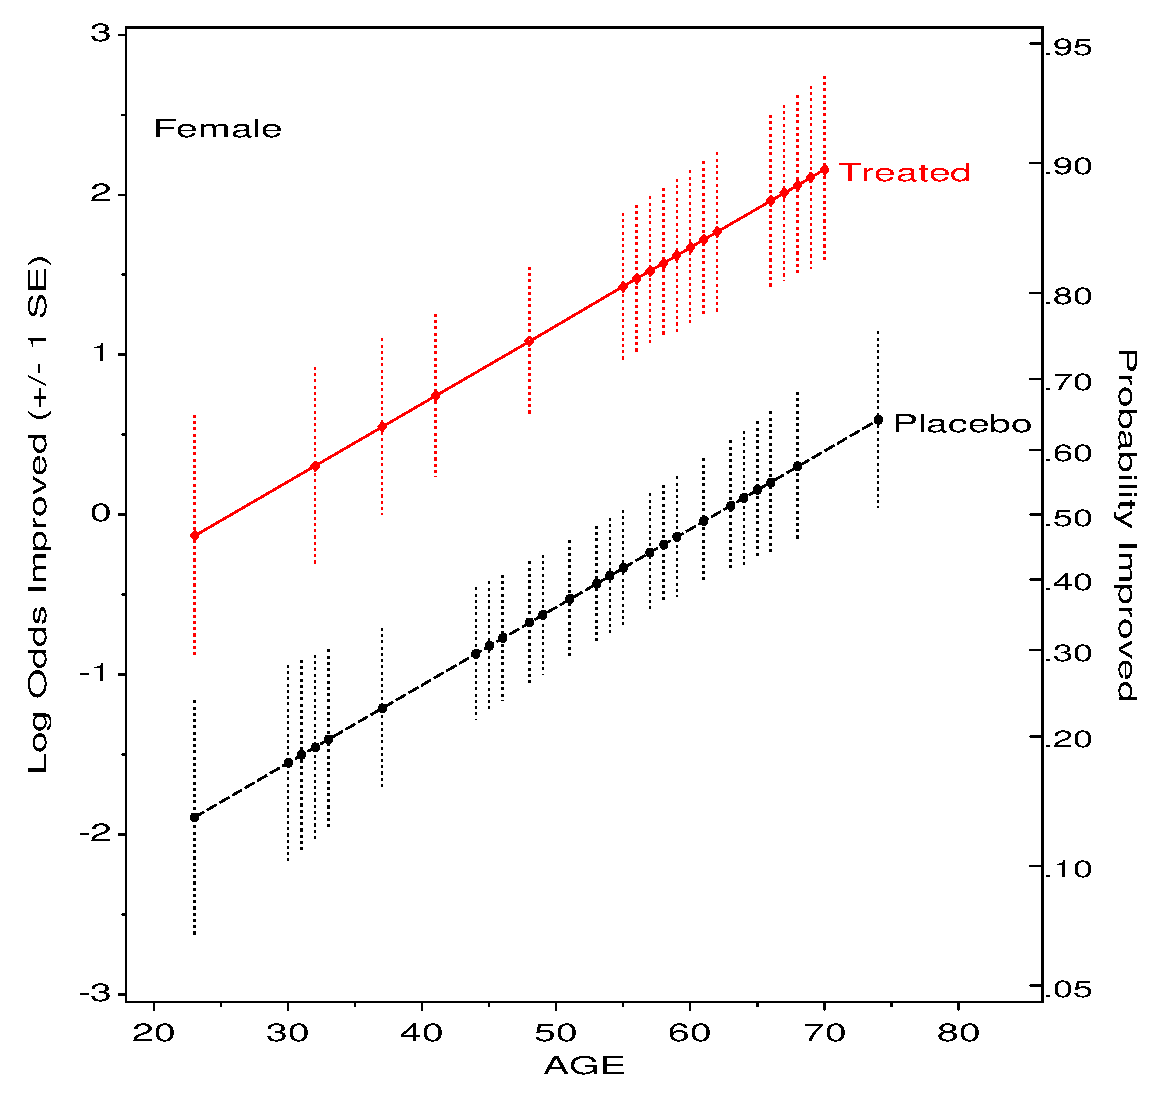
\includegraphics[width=1\linewidth]{ch6/fig/glogist1b1}
 \end{minipage}%
 \hfill
 \begin{minipage}[t]{.49\linewidth}
  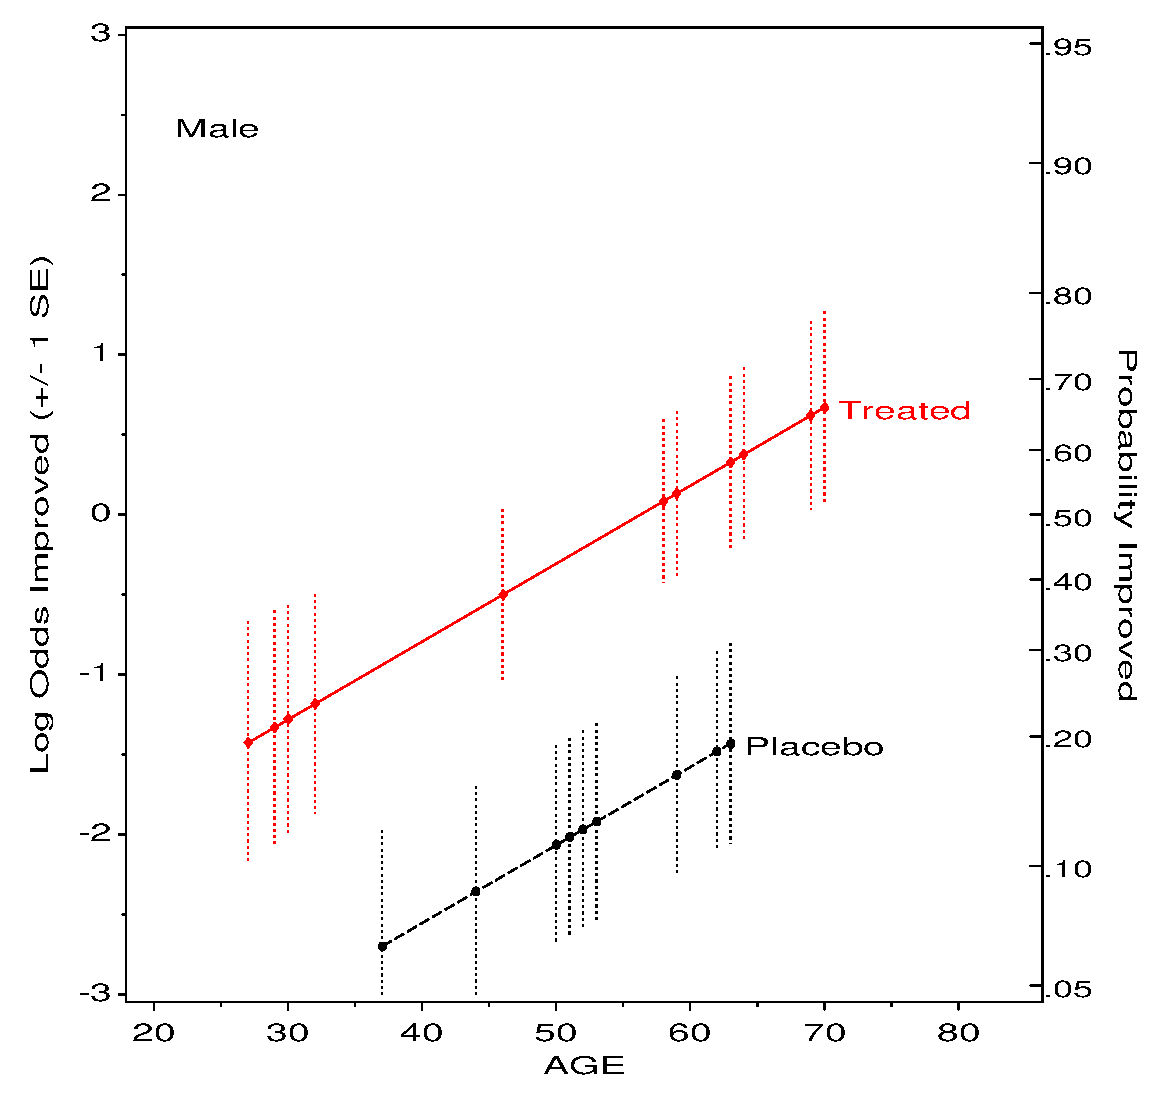
\includegraphics[width=1\linewidth]{ch6/fig/glogist1b2}
 \end{minipage}
 \caption[Estimated logits for sex, treatment and age]{Estimated logits for sex, treatment and age.
 Corresponding probabilities of a ``better'' response are shown on the right scale.}\label{fig:glogist1b}
\end{figure}

Predicted probabilities and confidence limits are contained in the
variables \texttt{PREDICT}, \texttt{UPPER}, and \texttt{LOWER}.
Corresponding logit values and their standard errors
are contained in the variables \texttt{LOGIT} and \texttt{SELOGIT}.
The predicted relations are linear and additive on the logit 
(log odds) scale
according to the model \eqref{eq:logisr},
but perhaps more interpretable on the probability scale.
One reasonable compromise is to plot the predicted log odds
along with an auxiliary scale showing the equivalent probability
values.

To show the
effects of sex, treatment, and age 
on improvement (Pr\{Better\}), 
separate plots
are drawn for each sex, using the statement \texttt{BY SEX;} in a 
\PROC{GPLOT} step.
These are shown side-by-side in \figref{fig:glogist1b},
facilitating their comparison.


Most of the work consists of drawing the confidence
limits with the Annotate facility, but this is worthwhile because it shows
the locations and bounds for individual observations.  
Plots of the predicted probabilities can
be made in a similar way using the variables
\texttt{PREDICT}, \texttt{UPPER}, and \texttt{LOWER}.

%% input: /Users/friendly/sasuser/catdata/glogist1b.sas
%% last modified: 27-Jul-99 15:36
\begin{listing}
proc sort data=results;
   by sex treat age;

data bars;
   set results(keep=sex treat age logit selogit);
   by sex treat;
   length text $8;
   xsys='2'; ysys='2';
   if treat='Placebo' then color='BLACK';
                      else color='RED';
   x  = age; line=33;
   y  = logit+selogit;  function='MOVE   '; output;
   y  = logit-selogit;
   y  = max(-3,y);      function='DRAW   '; output;
   if last.treat then do;
      y = logit;
      x = age+1; position='6';
      text = treat; function='LABEL'; output;
      end;
   if first.sex then do;
      ysys ='1'; y=90;
      xsys ='1'; x=10;
      text = sex; function='LABEL'; output;
      end;
\end{listing}

The probability scale is constructed using the \macro{PSCALE},
which produces an \ADS\ to draw the tick marks and probability
values along the right axis.  The axis label is drawn with a
\stmt{TITLE}{GPLOT} which specifies \pname{ANGLE=-90}.

%% input: /Users/friendly/sasuser/catdata/glogist1b.sas
%% last modified: 28-Jul-99 10:25
\begin{listing}
%pscale(anno=pscale);
data pscale;
   set pscale;
   sex = 'Female'; output;
   sex = 'Male  '; output;
proc sort;
   by sex;
data bars;
   set bars pscale;
   by sex;

title ' '
   h=1.5 a=-90 'Probability Improved'
   h=3.5 a=-90 ' ';
goptions hby=0;
proc gplot data=results;
   plot logit * age = treat / vaxis=axis1 haxis=axis2 hm=1 vm=1
                              nolegend anno=bars frame;
   by sex;
   axis1 label=(a=90 'Log Odds Improved (+/- 1 SE)')
         order=(-3 to 3);
   axis2 order=(20 to 80 by 10) offset=(2,6);
   symbol1 v=+ i=join l=3 c=black;
   symbol2 v=$ i=join l=1 c=red;
run;
\end{listing}

\figref{fig:glogist1b} provides a clear interpretation for the
predicted effects of age combined with those of treatment and
sex that we saw earlier.  On the logit scale, improvement increases
linearly with age.  The probability scale allows us to understand
the predicted values more readily.   For instance, we can see that
50 year-old woman given the active treatment
has a predicted probability of improvement
around 0.80, but a probability less than 0.40 if given the placebo.

Because the model includes no interaction terms, the fitted lines
are parallel for all treatment--sex groups, and the effects of all
variables are large compared to their standard errors.
However, we are only plotting fitted values here and should be
cautious until we have tested for interactions among these variables.
We do this in \secref{sec:logist-multint} (\exref{ex:arthrit11}).
\end{Example}
\begin{Example}[icu1]{Survival in the ICU}
In this example we examine briefly some aspects of logistic regression
related to model selection and graphical display with a mixture of
quantitative and discrete variables.
We use data from a study by
\citet{Lemeshow-etal:88}
of patients admitted to an intensive care unit at
Baystate Medical Center in Springfield,
Massachusetts.  The goal of this study was to develop a
model to predict the probability of survival (up to hospital
discharge) of these patients and to study the risk factors associated with 
ICU mortality.
Data for a sample of 200 subjects from this study are given in
\citet[App. 2]{HosmerLemeshow:89}, and reproduced in
\datref{dat:icu}.

There are 19 explanatory variables, of which three (age, systolic blood pressure and heart rate) are quantitative, one is categorical (race),
and the remaining 15 are binary (many having been dichotomized).
Initial model screening was carried out using the forward, backward,
and stepwise procedures using the \opt{SELECTION}{LOGISTIC}
on the \stmt{MODEL}{LOGISTIC}.  As in other model selection procedures,
it is prudent to regard these simply as ``candidate'' models,
nominated for further attention. 
The results for the full model with
all 19 predictors and for the final selection models are shown below.

\begin{center}
 \begin{tabular}{l rrrrr p{5.5cm}}
 \hline
  Selection & AIC & SC & $G^2$ & Score & df & Variables in Model \\ 
  \hline
  Full model & 160.78 & 226.74 & 79.38 & 74.74 & 19 & All \\ 
  Stepwise & 149.14 & 165.63 & 61.03 & 62.67 & 4 & Age Cancer Admit Uncons \\ 
  Forward & 149.14 & 165.63 & 61.03 & 62.67 & 4 & Age Cancer Admit Uncons \\ 
  Backward & 144.44 & 170.83 & 71.72 & 70.52 & 7 & Age Cancer Admit Uncons Systolic pH PCO \\ 
 \hline
 \end{tabular}
\end{center}

For the moment, we focus on the variables Age, Cancer, Admit
(elective vs.\ emergency admission) and
Uncons
(stupor or coma at admission).  These were nominated by all three procedures, and 
constitute the best model according to the forward and stepwise
procedures.  Estimated coefficients and odds ratios for this model
are shown in \outref{out:icu1.1}, fit using the statements below.
The lack of fit test (output not shown) gives $\chisq (8) = 5.081, p=0.74$,
showing no evidence of need for a more complex model.
\begin{listing}
%include data(icu);
proc logistic data=icu nosimple order=data;
     model died = age  cancer  uncons admit /
           scale=none aggregate lackfit;
     output out=results p=predict l=lower u=upper / alpha=.33;
\end{listing}

\begin{Output}[htb]
\caption{ICU data: Parameter estimates}\label{out:icu1.1}
\small
\verbatiminput{ch6/out/icu1.1}
\end{Output}
Because age is continuous, it is sensible to plot predicted
results against age, and to construct separate curves according
to the combinations of the other risk factors which are present
for each case.   A  composite variable \pname{risk} is created
combining the values of Cancer, Admit, and Uncons which all correspond
to increased risk of death.
\begin{listing}
data results;
   set results;
   length risk $16;
   if cancer then risk = 'Can';
   if admit  then risk = trim(risk) ||' Emerg';
   if uncons then risk = trim(risk) ||' Uncon';
   if risk =' ' then risk='None';
   risk = left(risk);
   label predict='Estimated Probability of Death';

proc sort;
   by risk age;
\end{listing}
The following steps create Annotate labels for the risk factors
and plot predicted probability of death for each combination,
producing the graph in \figref{fig:icu11}.
%% one figure
\begin{figure}[htb]
  \centering
  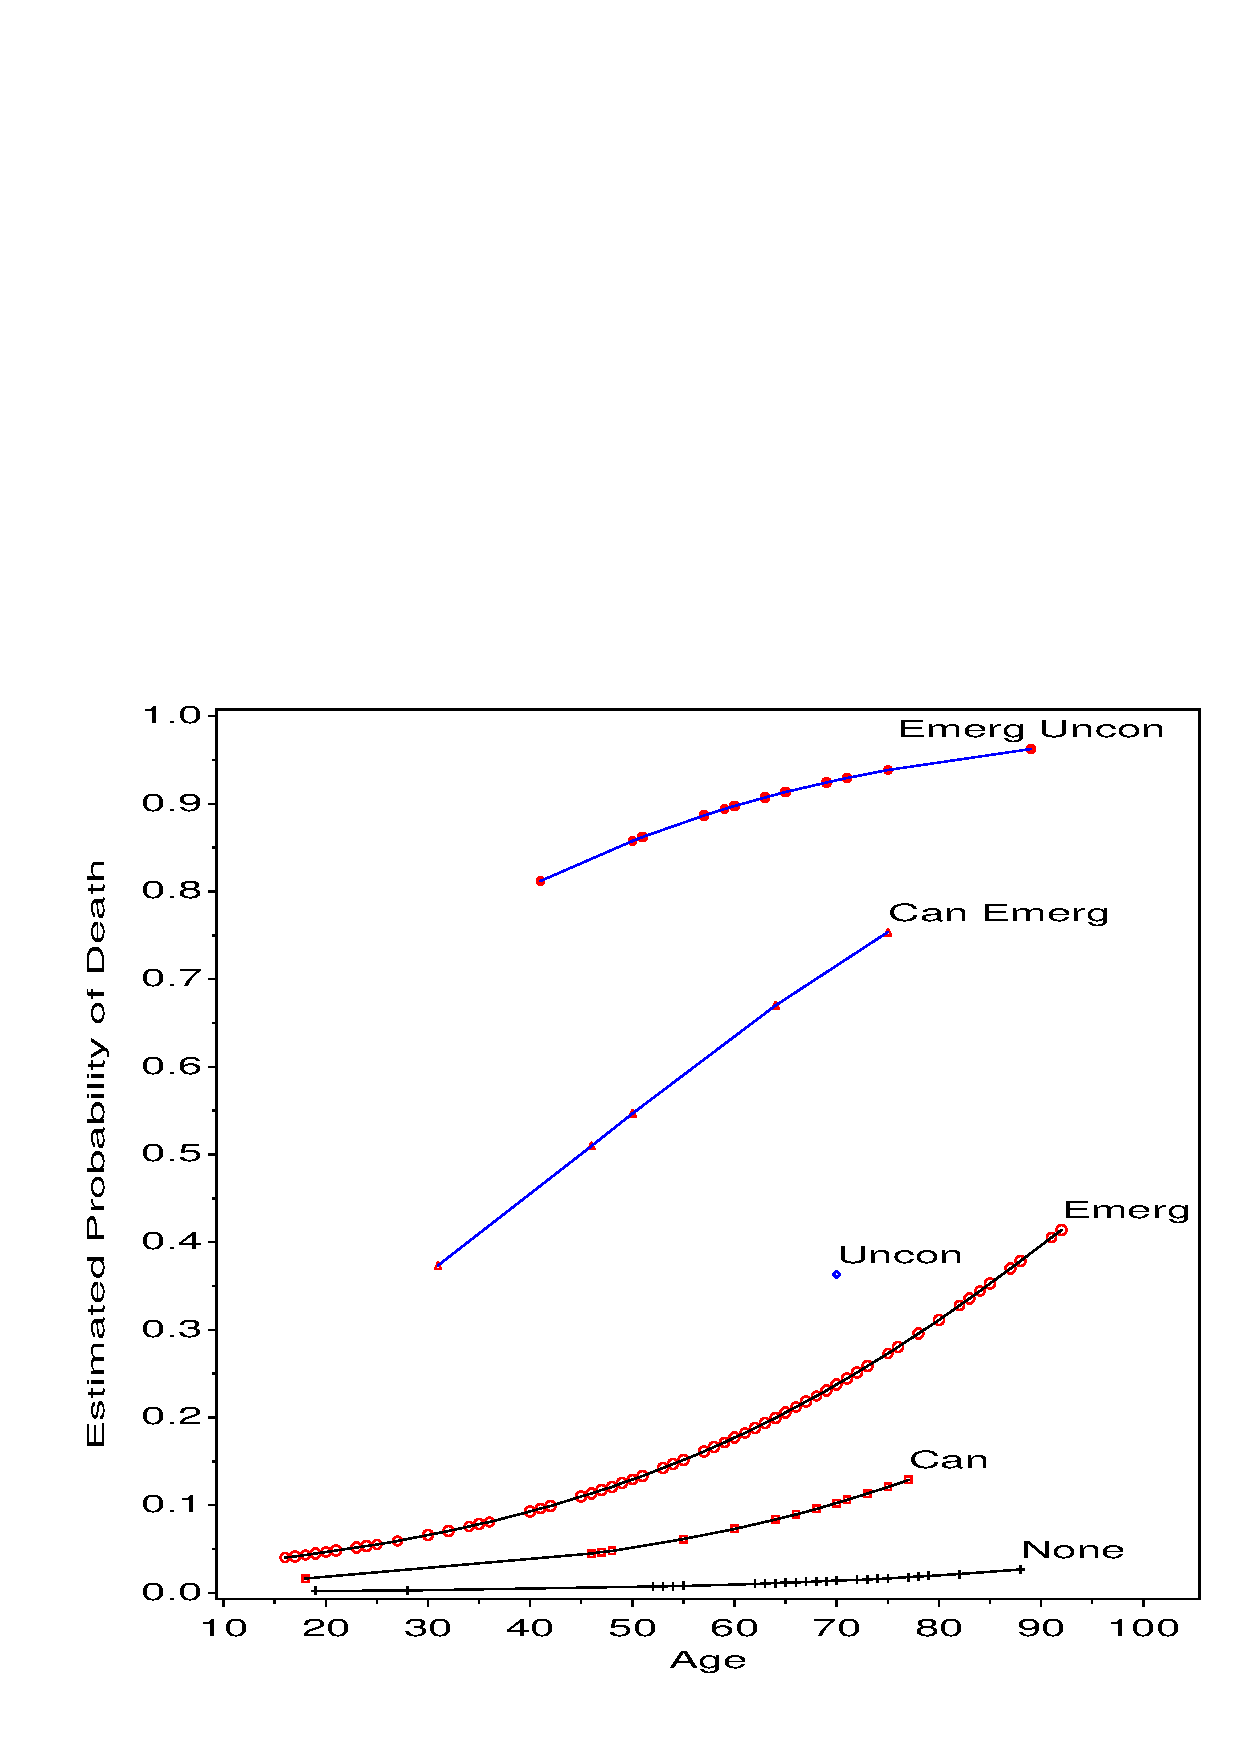
\includegraphics[scale=.6]{ch6/fig/icu11}
  \caption[ICU Survival data: Predicted probabilities]{ICU Survival data: Predicted probabilities for combinations of risk factors vs.\ age}%
  \label{fig:icu11}
\end{figure}
\begin{listing}
data label;
   set results;
   by risk;
   retain xsys ysys '2';
   position ='3';
   if predict>.9 then position='2';
   if last.risk then do;
      x = age;  y=predict;
      function = 'label   ';
      text=risk;
      output;
      end;

proc gplot data=results;
   plot predict * age = risk /
      frame anno=label vaxis=axis1 haxis=axis2 vm=1 hm=1 nolegend;
   axis1 label=(a=90);
   axis2 offset=(,4);
   symbol1 i=join v=square   c=red ci=black;
   symbol2 i=join v=triangle c=red ci=blue;
   symbol3 i=join v=circle   c=red ci=black;
   symbol4 i=join v=dot      c=red ci=blue;
   symbol5 i=join v=plus     c=black;
   symbol6 i=join v=diamond  c=blue ci=blue;
 run; quit;
\end{listing}
From the graph, it is apparent that mortality increases with
age when any of these risk factors are present, particularly
when the patient is admitted to Emergency; it is highest when the
patient is also unconscious at admission.  
From the odds ratios (see \outref{out:icu1.1}), we see that the
odds of death are increased 40-fold when the patient is unconscious.
The graph, however, shows the effects of these risk factors in
combination, and also indicates the number and age distribution of cases which have these combinations.

Before concluding that this model provides an adequate description of the
data, we should examine whether any individual cases are unduly influencing
the predicted results, and more importantly, the choice of variables in
the model.  We examine this question in \secref{sec:logist-infl}
where we return to these data (\exref{ex:icu2}).
\end{Example}

\subsection{Models with interaction}\label{sec:logist-multint}
The examples for the arthritis data have involved only main effects
of sex, age, and treatment.  We first illustrate tests for interactions
and powers of quantitative variables.
Whether interactions are present or not, the plotting of
estimated logits or predicted probabilities from \PROC{LOGISTIC} is no
more complicated in models with interactions.

In fact, since the predicted probabilities and logits are calculated
by the procedure and output to the \Dset\ \pname{RESULTS}, the results
plotted depend \emph{purely} on the \stmt{MODEL}{LOGISTIC}.  The plotting
steps remain the same as used in \figref{fig:glogist1b}, 
assuming you want to make separate plots for
males and females of the age by treatment effects.
For more complex models, or situations where you wish to plot predicted
results averaged over some variables, a method for plotting effects from
the model coefficients is described in \secref{sec:logistic-effplot}.

\begin{Example}[arthrit11]{Arthritis treatment}
The interaction effects were defined in the data step \pname{arthrit}
in \exref{ex:arthrit10} as
the dummy variables, \pname{agesex}, \pname{agetrt}, and \pname{sextrt}.  The
variable \pname{age2 = age**2} can be used to test whether the
relationship between age and logit(better) is quadratic rather than
linear.

A simple way to test for the need to include \emph{any} of these
more complex terms is illustrated here.
The \PROC{LOGISTIC} step below requests a forward-selection procedure.
Setting \pname{START=3} requests that the model building begin with the first
three variables (the main effects) listed in the model statement.
The option
\pname{SLENTRY=1} (significance level to enter) forces all variables to enter
the model eventually.

\begin{listing}
proc logistic data=arthrit;
   format better outcome.;
   model  better = _sex_ _treat_ age        /* main effects  */
                   agesex agetrt sextrt     /* interactions  */
                   age2                     /* quadratic age */
          / selection=forward
            start=3               /* start with main effects */
            slentry=1;           /* force all terms to enter */
\end{listing}

The variables included in each model for the selection procedure are
listed in a note at the beginning of each set of results:

\begin{output}
   Step  0. The following variables were entered:
            INTERCPT  _SEX_     _TREAT_   AGE
\end{output}

Results for this step are identical to those of the main effects
model given earlier.  Near the end of this step, the residual
\(\chi^2\) is printed, which corresponds to a joint test for the
other four variables.  This test is an appropriate test of goodness
of fit of the main effects model.

\begin{output}
   Residual Chi-Square = 4.0268 with 4 DF (p=0.4024)
\end{output}

Other tests printed show none of the interaction terms is significant
individually.
\end{Example}

\subsection{Effect plots from coefficients}\label{sec:logistic-effplot}
You can also construct plots for a fitted model
by calculating the predicted logit values directly from
the coefficients for the variables in the model.
This method can be used when raw data are not available, or when you
wish to average over certain effects to present simplified views of
a complex model.
To illustrate, for the arthritis
main effect model, the fitted relationship is
\begin{equation*}
  \logit ( p )  =
  - 4.5033  +
  1.4878 \,  \mbox{sex}   +
  1.7598 \,  \mbox{treat}  +
  0.0487 \,  \mbox{age}
  \period
\end{equation*}

With this method, the logit is calculated for each independent variable varied over its
range in all possible combinations.
Fixing an explanatory variable at its average gives an
effects plot for the remaining variables, which is particularly
useful when that
variable does not interact with others.
\citet{Fox:87} explains how this method may be used to construct adjusted
effects plots for particular interactions, adjusting for other
variables not represented in the plot.

The response can also be graphed on the probability scale by
transforming the logit via \(p = \exp(\logit) / ( 1  +  \exp(\logit) )\).  For example, the fitted logits and corresponding
probabilities for the arthritis data can be calculated in this data step:

\begin{listing}
data fitted;
  do _sex_ = 0 to 1;
     do _treat_ = 0 to 1;
        do age = 25 to 75 by 5;
           logit= -4.5033 + 1.4878*_sex_ + 1.7598*_treat_ + 0.0487*age;
           prob = exp(logit) / (1 + exp(logit));
           output;
           end;
        end;
     end;
\end{listing}
Replacing the outer \pname{DO}-loop with \verb|_sex_| = $\Pr_{\mbox{\scriptsize Female}} = 59/84 = .702$
would give fitted values at the average over sex; using \verb|_sex_| = 1/2
would give fitted values for a population with an equal sex distribution.

\begin{Example}[davis]{Volunteering for a psychological experiment}
\citet{Fox:87} illustrated this method using data from a study by \citet{CowlesDavis:87} on the personality factors which predispose
people to volunteer for a psychological experiment.
In this study, 1421 university students completed a personality inventory,
which contained a 24-item scale of Introversion-Extroversion
and a 24-item scale of Stability-Neuroticism, among other measures.
They were also asked to indicate their willingness in principle to
volunteer for a psychological experiment, which was the response to
be explained by the personality variables.

Fox reports the results of a logistic regression fit to these data
as
\begin{equation*}
\logit ( \pi_v ) = -2.605 + 0.2472 \mbox{ Sex} + 0.1668 E + 0.1108 N - 0.0088552 E \times N \quad ,
\end{equation*}
where $\pi_v$ is the probability of volunteering, Sex is a dummy variable
coded 0 for males and 1 for females, $E$ is the Introversion-Extroversion
score on a scale of 0--24, and $N$ is the Stability-Neuroticism score,
also on a scale of 0--24.

In this model, the positive coefficient for sex implies that women are
more likely to volunteer than men at each combination of extroversion
and neuroticism.
Because sex does not interact with either extroversion or neuroticism
we may focus on the relation between the probability of volunteering
and the two personality variables.
Setting \pname{sex=.5} in the \Dstp\ below generates observations
for the adjusted effects in a population equally composed of men and women.%
\footnote{Alternatively, we could set \pname{sex=0.55},
the proportion of women in the sample.}
\begin{listing}
data predict;
   array b\{0:4\} _temporary_ (-2.605  0.2472  0.1668  0.1108 -0.008552);
   do sex = 0 to 1 by .5;
      do neurot = 0 to 24 by 6;
         do extra = 0 to 24 by 6;
            logit = b[0] + b[1]*sex + b[2]*extra + b[3]*neurot
                  + b[4]*extra*neurot;
            prob = exp(logit) / ( 1 + exp(logit) );
            output;
            end;
         end;
      end;
\end{listing}

At a given level of sex, we may graph the fitted probability of volunteering
(\pname{prob}) against one predictor (say, extroversion) with separate
curves for each level of the other predictor (neuroticism).
The graph for the average over sex is shown in \figref{fig:davisn2}.
First, we may find the average probability of volunteering
by averaging the logits and transforming the average values to the
probability scale.
%% one figure
\begin{figure}[htb]
  \centering
  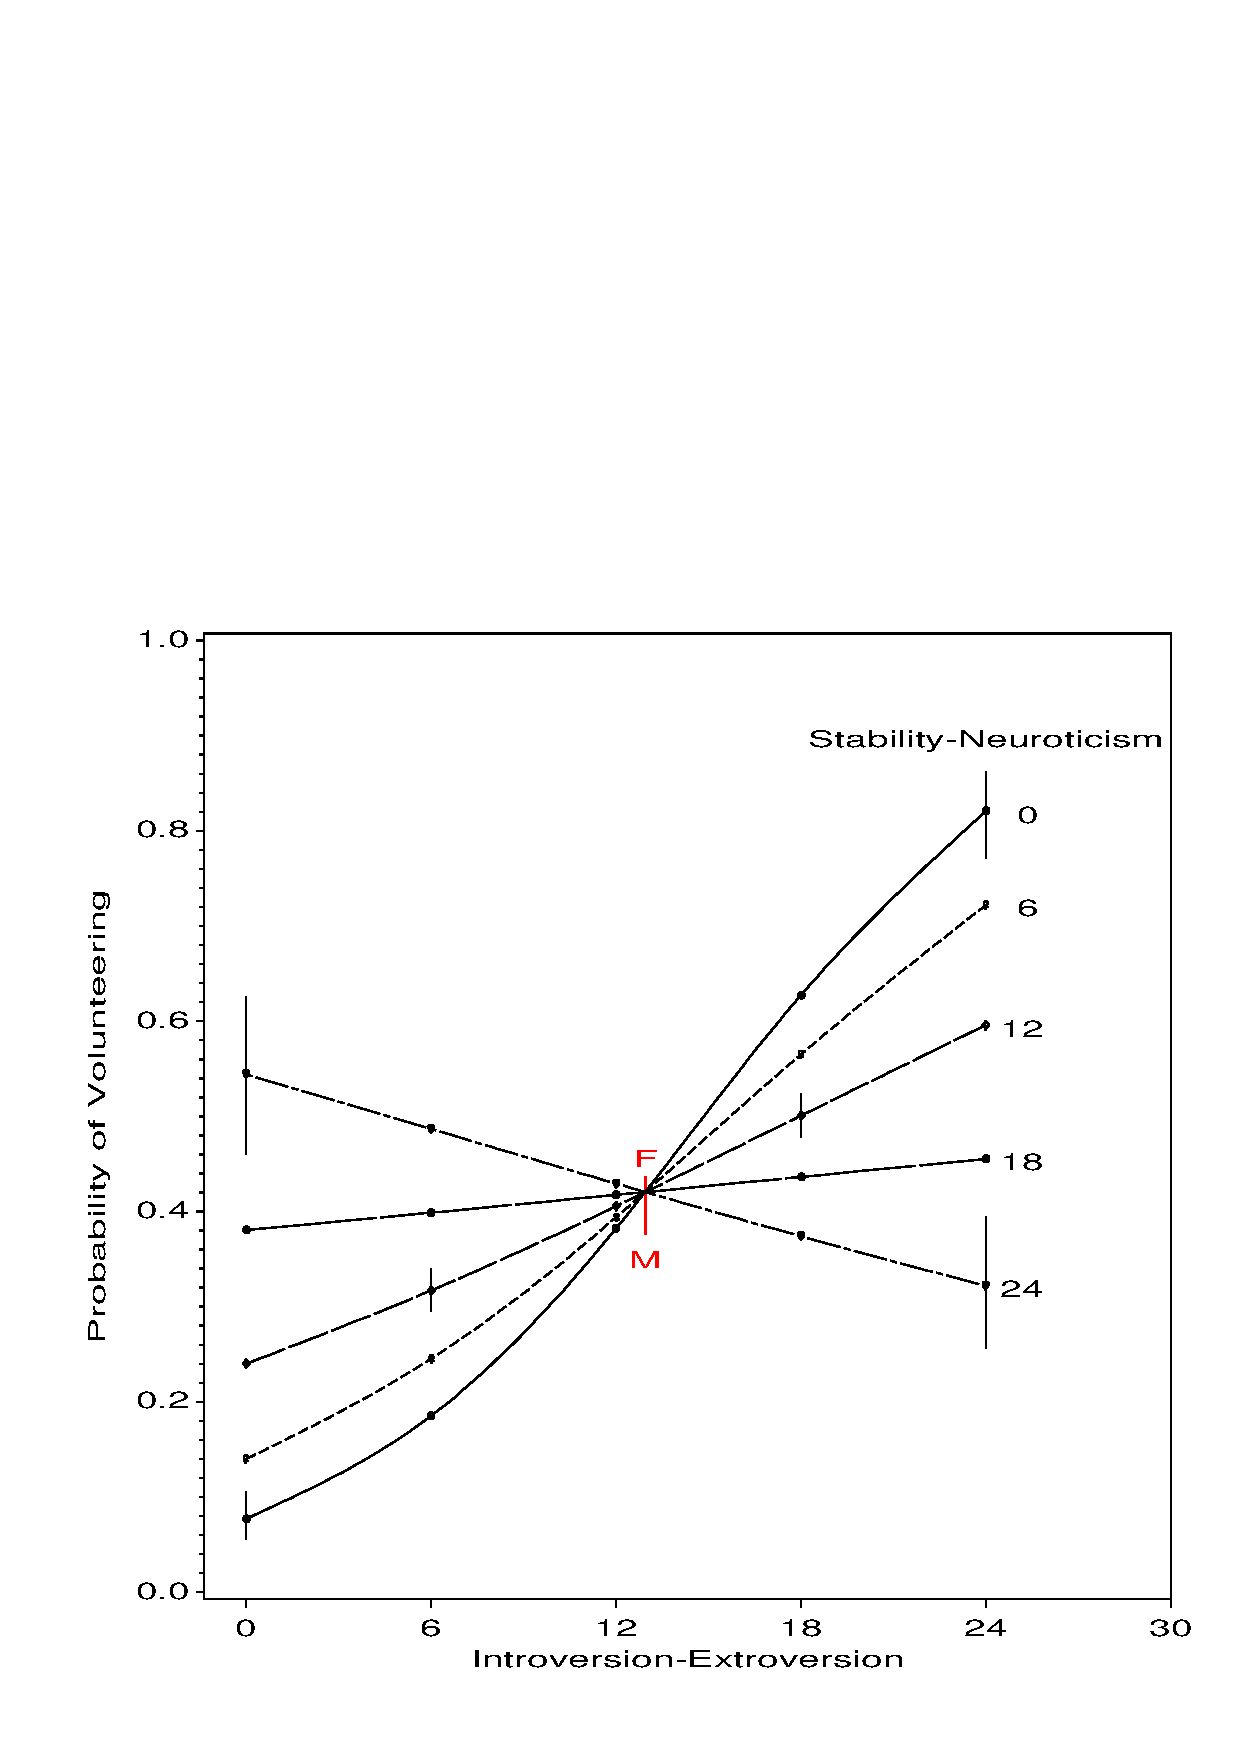
\includegraphics[scale=.6]{ch6/fig/davisn2}
  \caption[Fitted probability of volunteering, controlling for sex]{Fitted probability of volunteering, controlling for sex.  The effect of sex is shown
  at the point where the curves intersect.  The vertical lines at other
  selected combinations of extroversion and neuroticism show individual
  50\% confidence intervals.}%
  \label{fig:davisn2}
\end{figure}
\begin{listing}
proc summary nway data=predict;
   class sex;
   var logit ;
   output out=means mean=;
data means;
   set means;
   drop _type_ _freq_;
   prob = exp(logit) / (1 + exp(logit));
proc print;
\end{listing}
which gives
\begin{output}
                     OBS    SEX      LOGIT       PROB

                      1     0.0    -0.50587    0.37616
                      2     0.5    -0.38230    0.40557
                      3     1.0    -0.25872    0.43568
\end{output}
The statements below create an \ADS\ which supplies the labels
for the levels of neuroticism in the figure.
The effect of sex is shown by drawing a vertical line
showing the average probability of volunteering for men and for women
at the center of the graph.
\begin{listing}
proc format;
   value sex 0='Male'
            .5=' '           /* average */
             1='Female';
data anno;
   set predict;
   by sex neurot;
   xsys='2'; ysys='2';
   length text $22 function color $8;
   position='5';
   if last.neurot then do;
      x=extra+1;
      y=prob;
      text = put(neurot,3.0); function='LABEL'; output;
      end;

   if first.sex then do;
      y=.90;
      x=24; text='Stability-Neuroticism';
      function='LABEL'; output;
      x=2; text=put(sex,sex.);
      function='LABEL'; output;
      if text =' ' then do;
         color = 'red';
         x = 12.956;                * intersection of curves;
         y = 0.43568;               * average prob for females;
         function = 'MOVE '; output;
         text = 'F'; position = '2';
         function = 'LABEL' ; output;
         y = 0.37616;               * average prob for males;
         function = 'DRAW ' ; output;
         text = 'M'; position = '8';
         function = 'LABEL' ; output;
         end;
      end;
\end{listing}
The graph in \figref{fig:davisn2} is the second of three panels 
(for \pname{SEX=0.5}) drawn by the
\PROC{GPLOT} step below.
The other two graphs have the same form, shifted up for females
and down for males, as indicated by the vertical bar at the
intersection of the curves in \figref{fig:davisn2}.
\begin{listing}
goptions hby=0;
proc gplot data=predict;
   plot  prob * extra = neurot /
         vaxis=axis1 haxis=axis2 hminor=0
         frame nolegend anno=anno;
   by sex;
   axis1 label=(a=90) order=(0 to 1 by .2);
   axis2 label=(h=1.5 'Introversion-Extroversion')
         order=(0 to 30 by 6)  offset=(3,0);
   symbol1 v=+ i=spline l=1 c=black;
   symbol2 v=* i=spline l=3 c=black;
   symbol3 v=$ i=spline l=5 c=black;
   symbol4 v=- i=spline l=7 c=black;
   symbol5 v=# i=spline l=9 c=black;
\end{listing}
The interpretation of these results is quite clear from the graph.
At low levels of neuroticism, probability of volunteering increases
with extroversion, but the slope of this relation decreases
as neuroticism increases.
(If you want a lot of volunteers in a psychological experiment,
look for extraverted non-neurotics.)
At the highest levels of neuroticism,
probability of volunteering decreases with extroversion.

The error bars shown in \figref{fig:davisn2} require the estimated
variance-covariance matrix of the coefficients, $\widehat{\mathcal{V} (\vec{b})} = (\mat{X}\trans \mat{V} \mat{X})^{-1}$,
in addition to the coefficients themselves.
Because the fitted value, $\logit (\pi_i) = \vec{x}_i \trans \vec{b}$,
 is a linear combination of the parameters,
its standard error may be calculated as
\begin{equation*}
\mbox{s.e.} \logit (\pi_i) =
 [ \vec{x}_i \trans \widehat{\mathcal{V} (\vec{b})} \vec{x}_i ] ^ {1/2}
\end{equation*}
An approximate 50\% confidence interval for the fitted logit may
then be calculated as $\logit (\pi_i) \pm 0.67 \times \mbox{s.e.} \logit (\pi_i)$,
and the end points transformed back to the probability scale.

For example, the \Dstp\ below read the coefficients and the estimated
variance-covariance matrix in the form it would be produced by
\PROC{LOGISTIC} with the options \pname{OUTEST=PARMS COVOUT}
on the \pname{PROC} statement.
\begin{output}
data parms;
   input _type_ $ _name_ $ intercep sex extra neurot extneu;
datalines;
PARMS   ESTIMATE  -2.60551   0.24715   0.16682   0.11078  -.0085525
COV     INTERCPT   0.27504  -0.01839  -0.01819  -0.01726  0.0012943
COV     SEX       -0.01839   0.01246   0.00013  -0.00007  -.0000134
COV     INTEXT    -0.01819   0.00013   0.00142   0.00127  -.0001023
COV     NEUROT    -0.01726  -0.00007   0.00127   0.00142  -.0001052
COV     EXTNEU     0.00129  -0.00001  -0.00010  -0.00011  0.0000086
;
\end{output}
(If this analysis was carried out using raw data, the \pname{OUTEST=PARMS}
\Dset\ could be used directly.)
Calculation of the standard errors and confidence intervals is
then done most easily with \IML, as follows:
%\begin{changebar}
\begin{listing}
proc iml;
   use parms;
   read var\{intercep sex extra neurot extneu\} into b where(_type_='PARMS');
   read all var\{intercep sex extra neurot extneu\} into cov
       where(_type_='COV');
   b = t(b);
   do sex = 0 to 1 by .5;
      do neurot = 0 to 24 by 6;
         do extra = 0 to 24 by 6;
            x = 1 || sex || extra || neurot || extra#neurot;
            logit = x * b;
            selogit = sqrt( x * cov * t(x) );
            prob = exp(logit) / ( 1 + exp(logit) );
            result = result // ( x[,2:4] || logit || selogit || prob );
            end;
         end;
      end;
  ul = result[,4] + .67#result[,5];
  ll = result[,4] - .67#result[,5];
  lower = exp(ll) / ( 1 + exp(ll) );
  upper = exp(ul) / ( 1 + exp(ul) );
  var = \{sex extra neurot logit selogit prob lower upper\};
  result = result || lower || upper;
  create predict from result[c=var];
  append from result;
quit;
\end{listing}
%\end{changebar}
The error bars in \figref{fig:davisn2} serve notice that the predicted
probabilities are most precise for those with average levels of
the explanatory variables, as is usual with linear models.
\end{Example}

\section{Influence and diagnostic plots}\label{sec:logist-infl}

In ordinary least squares (OLS) regression, measures of \glossterm{influence}
(leverage, Cook's D, DFBETAs, etc.) help you to determine whether
individual cases (or cells in grouped data)
have undue impact on the fitted regression model and
the coefficients of individual predictors.
Analogs of most of these
measures have been suggested for logistic regression.
\citet{Pregibon:81} provided the theoretical basis for these methods,
exploiting the relationship between logistic models and
weighted least squares.  Some
additional problems occur in practical applications to
logistic regression because the response
is discrete, and because the leave-one-out diagnostics are more
difficult to compute.

\subsection{Residuals and leverage}
\ix{logistic regression!residuals|(}
As in ordinary least squares regression, the influence (actual impact)
of an observation in logistic models depends multiplicatively
on its residual (disagreement between $y_i$ and $\hat{y}_i$)
and its leverage (how unusual $\vec{x}_i$ is in the space of the
explanatory variables).
The multiplicative definitions imply that a case is influential to
the extent that it is poorly fit \emph{and} has unusual values of
the predictors.

In logistic regression, the simple raw residual is just $e_i \equiv y_i - \hat{p}_i$,
where $ \hat{p}_i = \exp( \vec{x}_i\trans \vec{b} ) / [1 + \exp( \vec{x}_i\trans \vec{b} )]$.
The  Pearson and deviance residuals are more useful for identifying
poorly fitted observations, and are components of overall goodness-of-fit
statistics.
The \boldital{Pearson residual} is defined as
\begin{equation}\label{eq:reschi}
r_i \equiv \frac{e_i}{\sqrt{ p_i  (1-p_i)}}
\end{equation}
and the Pearson chi-square is therefore $\chisq = \sum r_i^2$.
The \boldital{deviance residual} is
\begin{equation}\label{eq:resdev}
g_i \equiv \pm { -2 [ y_i \log p_i  + (1-y_i) \log (1-p_i) ] }^{1/2}
\end{equation}
where the sign of $g_i$ is the same as that of $e_i$.
Likewise, the sum of squares of the deviance residuals gives
the overall deviance,
$G^2 = -2 \log \mathcal{L}(\vec{b}) = \sum g_i^2$.

When $y_i$ is a binomial count based on $n_i$ trials (grouped data),
the Pearson residuals \eqref{eq:reschi} then become
\begin{equation*}%\label{eq:reschi2}
r_i \equiv \frac{y_i -n_i p_i}{\sqrt{n_i  p_i  (1-p_i)}}
\end{equation*}
with similar modifications made to \eqref{eq:resdev}.
\ix{logistic regression!residuals|)}

\ix{logistic regression!leverage|(}
Leverage measures the \emph{potential} impact of an individual case
on the results, which is directly proportional to how far an
individual case is from the centroid in the space of the
predictors.  Leverage is computed as the diagonal elements,
\(h_{ii}\), of the ``Hat'' matrix, \(\mat{H}\),

\begin{equation*}%\label{eq:}
\mat{H} = {\mat{X}}^\star
{( {\mat{X}^\star}\trans {\mat{X}}^\star )}^{-1} {\mat{X}^\star}\trans
\end{equation*}
where \({\mat{X}} ^\star = {\mat{V}}^{1/2} \mat{X}\), and \(\mat{V}  =
\diag [ \hat{\vec{p}} ( 1 - \hat{\vec{p}})] \).  As in OLS,
leverage values are between 0 and 1, and a leverage value,
\(h_{ii}  > 2 (k+1) /  n\) is considered ``large''; here, \(k\) is the
number of predictors, and \(n\) is the number of cases.
In OLS, however, the hat values depend only on the $X$s, whereas
in logistic regression, they also depend on the dependent
variable values and the fitted probabilities (through $\mat{V}$).
As a result, an observation may be extremely unusual on the predictors,
yet not have a large hat value, if the fitted probability is near 0 or 1.
\ix{logistic regression!leverage|)}

\subsection{Influence diagnostics}\label{sec:logist-infldiag}
\ix{logistic regression!influence diagnostics|(}
Influence measures assess the effect that deleting an
observation has on the regression parameters, fitted values, or the
goodness-of-fit statistics.  In OLS, these measures
can be computed exactly from a single regression.
In logistic regression, the exact effect of deletion
requires refitting the model with each observation deleted in turn
(because the estimating equations \eqref{eq:like4} are nonlinear),
a time-intensive computation.
Consequently, \citet{Pregibon:81} showed how analogous deletion
diagnostics may be approximated by performing one additional step
of the iterative procedure.

The simplest measure of influence of observation $i$ is the standardized change in the coefficient for each variable due to omitting that observation,
termed \boldital{DFBETA}s.  From the relation \citep[p. 716]{Pregibon:81}
\begin{equation*}%\label{eq:dfbetas}
 \vec{b} -  \vec{b}_{(-i)} = (\mat{X}\trans \mat{V} \mat{X})^{-1} \vec{x}_i (y_i - p_i) / (1 - h_{ii})
 \comma
\end{equation*}
the estimated standardized change in the coefficient for variable $j$ is
\begin{equation}\label{eq:dfbeta}
 \mbox{DFBETA}i_j \equiv \frac{b_{(-i)j} -  b_j } {\hat{\sigma} (b_j)}
 \comma
\end{equation}
where $\hat{\sigma} (b_j)$ is the estimated standard error of $b_j$.
With $k$ regressors, there are $k+1$ sets of DFBETAs, which makes their examination burdensome.
Graphical displays ease this burden, as do various summary measures
considered below.

The overall influence of observation $i$ on the estimated regression
coefficients is assessed by analogs of \glossterm{Cook's distance}, which measure
the difference between $\vec{b}$ for all the data and
$\vec{b}_{(-i)}$ estimated without observation $i$.
One measure, $C_i$, is defined as
\begin{equation*}%\label{eq:cookd1}
C_i \equiv ( \vec{b} - \vec{b}_{(-i)} )\trans \:
    \mat{X}\trans \mat{V} \mat{X} \:
     ( \vec{b} - \vec{b}_{(-i)} )
	  \comma
\end{equation*}
and calculated as
\begin{equation}\label{eq:cookd2}
 C_i = \frac{r_i^2 h_{ii}} {(1-h_{ii} )^2}
 \period
\end{equation}
A second measure, $\overline{C}_i$, is calculated as
\begin{equation}\label{eq:cookd3}
 \overline{C}_i = \frac{r_i^2 h_{ii}} {(1-h_{ii} )} = (1-h_{ii} ) C_i
 \period
\end{equation}
Because $0 \le h_{ii} \le 1$, $\overline{C}_i$ will never be larger than $C_i$.
These measures are referred to by the keywords \pname{C} and
\pname{CBAR}, respectively, on the \stmt{OUTPUT}{LOGISTIC}.
Both can be interpreted as squared measures of the change in
size of the confidence intervals for all regression coefficients.
Rules of thumb for noticeably large values are necessarily only
rough indicators, but \citet{Johnson:85} suggests comparing $k C_i$
to a $\chi^2 (k)$ distribution.

The Pearson and deviance residuals defined above do not have equal
variance, but rather have variance $\approx 1-h_{ii}$.  Studentized versions
of both which do have equal variance
are obtained by dividing by $\sqrt{1-h_{ii}}$.  For example, the
studentized deviance residual (\pname{RESDEV}) is $g_i^\star = g_i /
\sqrt{1-h_{ii}}$.
These are most usefully expressed in squared form as the approximate decrease in the
deviance (\pname{DIFDEV}) and Pearson (\pname{DIFCHISQ}) \chisq\ 
associated with deleting observation $i$:
\begin{equation*}%\label{eq:difdev}
  \Delta G_{(-i)}^2 = \frac{g_i^2}{1-h_{ii}}
  \comma
\end{equation*}
and
\begin{equation*}%\label{eq:chi}
  \Delta \chi_{(-i)}^2 = \frac{r_i^2}{1-h_{ii}}
  \period
\end{equation*}
These are both asymptotically distributed as $\chi^2 (1)$, so a value
exceeding 3.84 (or the rounded value, 4) is worth noticing.
They may also be interpreted as indicating how poorly the current
model fits observation $i$.

As with OLS, influential observations signal something unusual:
extreme (or erroneous) predictor values combined with an ill-predicted
response, e.g., someone who died, but should have survived (according to the
model).  They may also signal that some important (perhaps unmeasured)
predictor--- a lurking variable--- has been omitted from the model \citep{Joiner:81} or expressed
on the wrong scale.

\subsection{Influence output from \PROC{LOGISTIC}}
All the influence statistics are
printed when the \opt{influence}{LOGISTIC} is used on the \stmt{MODEL}{LOGISTIC}.
For example, we get these diagnostics for the arthritis data with:
\begin{listing}
proc logistic data=arthrit ;
   model better = _sex_ _treat_ _age_ / influence;
\end{listing}

This produces many pages of output, of the form in \outref{out:glogist3.1},
shown for two of the many diagnostic measures.
With so much output, it is often difficult
to spot unusual observations.  A more useful option, \pname{IPLOTS},
produces index plots of each of the diagnostic measures against
the observation index, with the goal of showing which observations
stand out from the rest.
It is even more useful, I believe, to plot certain diagnostics
against each other, including reference lines showing the nominal
danger-level for each diagnostic,  because they help to pinpoint
\emph{why} certain observations are influential.
Some examples of these plots are described in the following subsection.

\begin{Output}[htbp]
\caption{Regression diagnostics, printed output (partial) for arthritis data}\label{out:glogist3.1}
\small
\verbatiminput{ch6/out/glogist3.1}
\end{Output}

\subsection{Diagnostic plots of influence measures}
Plots of the change in \(\chi^2\) (\pname{DIFCHISQ} or \pname{DIFDEV}) against
either leverage or predicted probability are particularly useful
for detecting unduly influential cases.
These are discrete analogs of plots recommended for linear models
by \citet{Fox:91} and \citet{Friendly:91}.
The estimated overall
influence of each case on the estimated coefficients ($C_i$ or $\overline{C}_i$)
can be shown in a bubble plot where the plotting symbols are circles
proportional to \pname{C} or \pname{CBAR}.

Such plots are produced by the \macro{INFLOGIS},
described in \macref{mac:inflogis}.  For example, these
statements produce plots of DIFCHISQ against both the 
predicted probability, \pname{PRED} 
(\figref{fig:logi1b1}) and
leverage, \pname{HAT}
(\figref{fig:logi1b2}),
using bubbles whose area is proportional
to C:
%% \input{logist1b} %% level: 2
\begin{listing}
title 'Arthritis treatment data';
title2 'Bubble size: Influence on Coefficients (C)';
goptions htext=1.6;
%include data(arthrit);
%inflogis(data=arthrit,
     y=better,               /* response   */
     x=_sex_ _treat_ age,    /* predictors */
     id=id,                  /* case label */
     gy=DIFCHISQ,            /* graph ordinate  */
     gx=PRED HAT,            /* graph abscissas */
     lcolor=RED, bsize=14
     );
\end{listing}

The printed output from the \macro{INFLOGIS} includes a table
identifying any observation of high leverage \emph{or} high influence.
These observations are also labeled in the graphs.  For
example, case 29 is of high leverage, because she is unusual in terms
of the predictors: a young woman given treatment; however, she is not
influential in the fitted model.  Case 77, is not of high leverage,
but is poorly predicted by the model and has a large contribution to
\chisq.

\begin{output}
CASE BETTER  _SEX_  _TREAT_  AGE   HAT  DIFCHISQ   DIFDEV     C

  1     1      0       1      27   .09    4.5781   3.6953   0.4510
 22     1      0       0      63   .06    4.4603   3.5649   0.2898
 29     0      1       1      23   .14    1.0183   1.4005   0.1679
 30     1      1       0      31   .05    4.7485   3.6573   0.2611
 34     1      1       0      33   .05    4.2955   3.4644   0.2236
 55     0      1       1      58   .03    4.9697   3.6759   0.1602
 77     0      1       1      69   .03    8.4977   4.7122   0.2758
\end{output}

\begin{figure}[!htb]
  \centering
  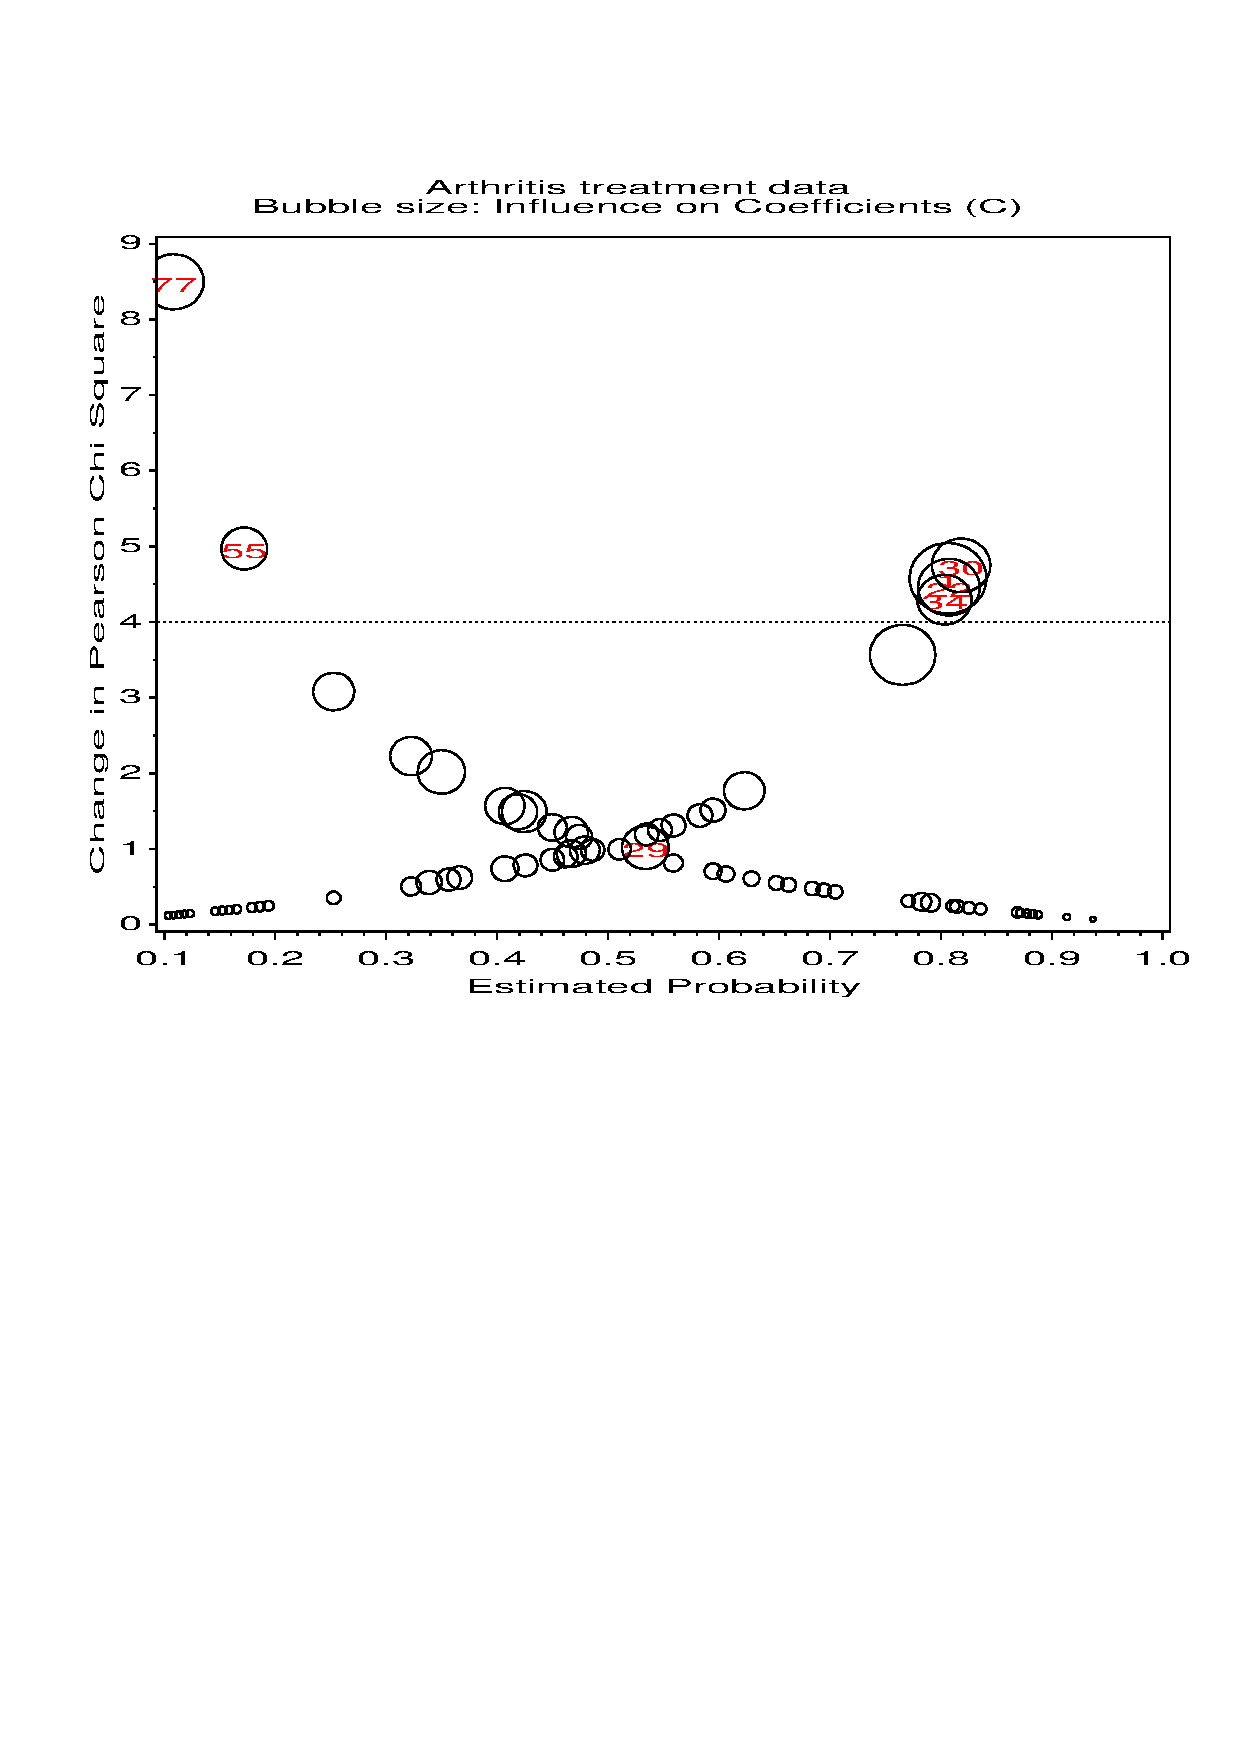
\includegraphics[scale=.7]{ch6/fig/logist1b1}
  \caption[Influence plot for arthritis data]{Influence plot for arthritis data.
Cases with DIFCHISQ \(> 4\) or leverage \(>  (2 k) /  n  = 0.095\) are
labeled as
influential, as indicated by the size of the bubble symbol.
The systematic pattern shown is inherent in the discrete nature of
logistic regression.  The most influential
observations are those with very high or low predicted probabilities.}\label{fig:logi1b1}
\end{figure}

\begin{figure}[!htb]
  \centering
  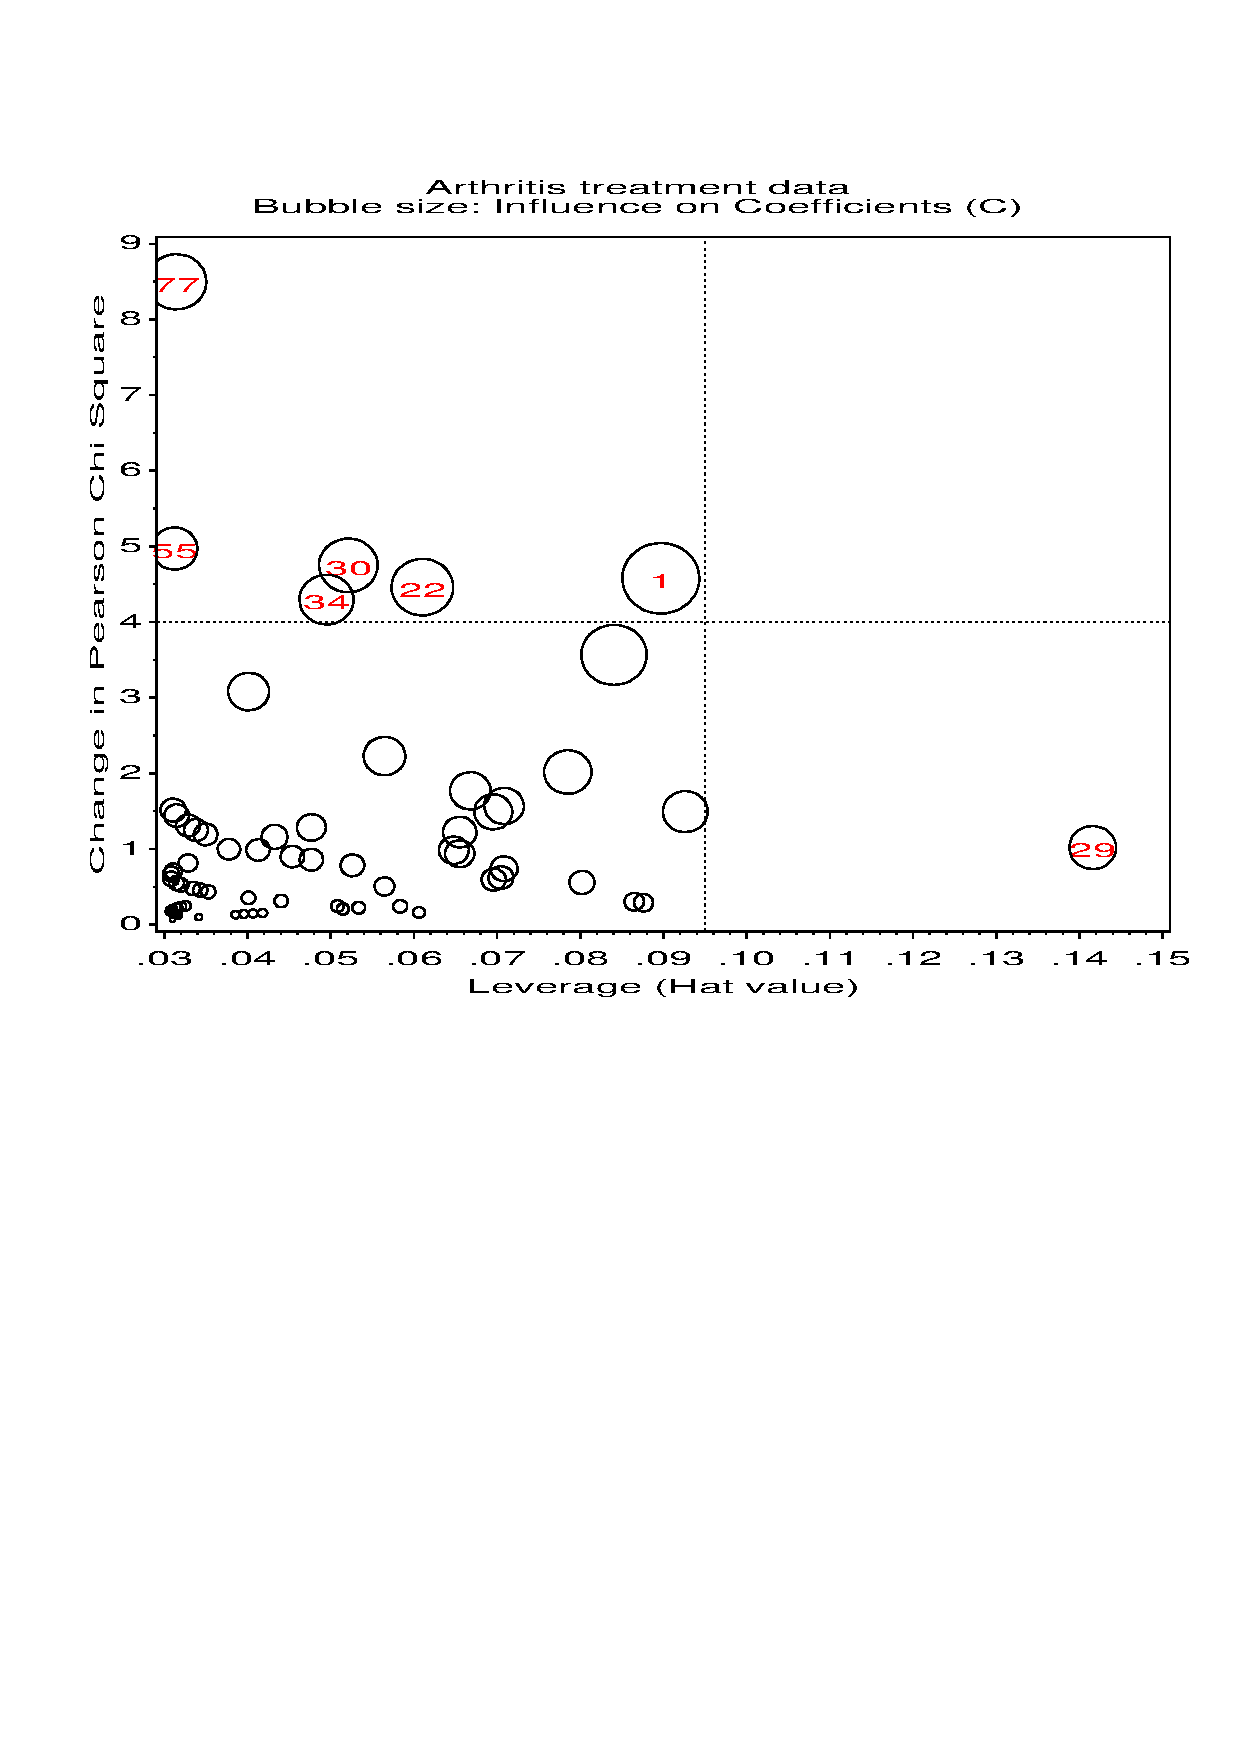
\includegraphics[scale=.7]{ch6/fig/logist1b2}
  \caption[Changes in chi-square vs. leverage]{Changes in chi-square vs.\ leverage.
  The same cases are labeled as in \figref{fig:logi1b1}.
}\label{fig:logi1b2}
\end{figure}
\ix{logistic regression!influence diagnostics|)}

\begin{Example}[icu2]{Survival in the ICU}
The four variable model from \exref{ex:icu1} predicting survival in the ICU
was examined for influential cases with the \macro{INFLOGIS}.
The following macro call produces an influence plot of the \pname{DIFCHISQ}
statistic against hat values, shown in \figref{fig:icu12}.
\begin{listing}
%inflogis(data=icu, y=died, x=age cancer uncons admit,
   id=id,
   gy=difchisq,
   gx=hat);
\end{listing}

%% one figure
\begin{figure}[htb]
  \centering
  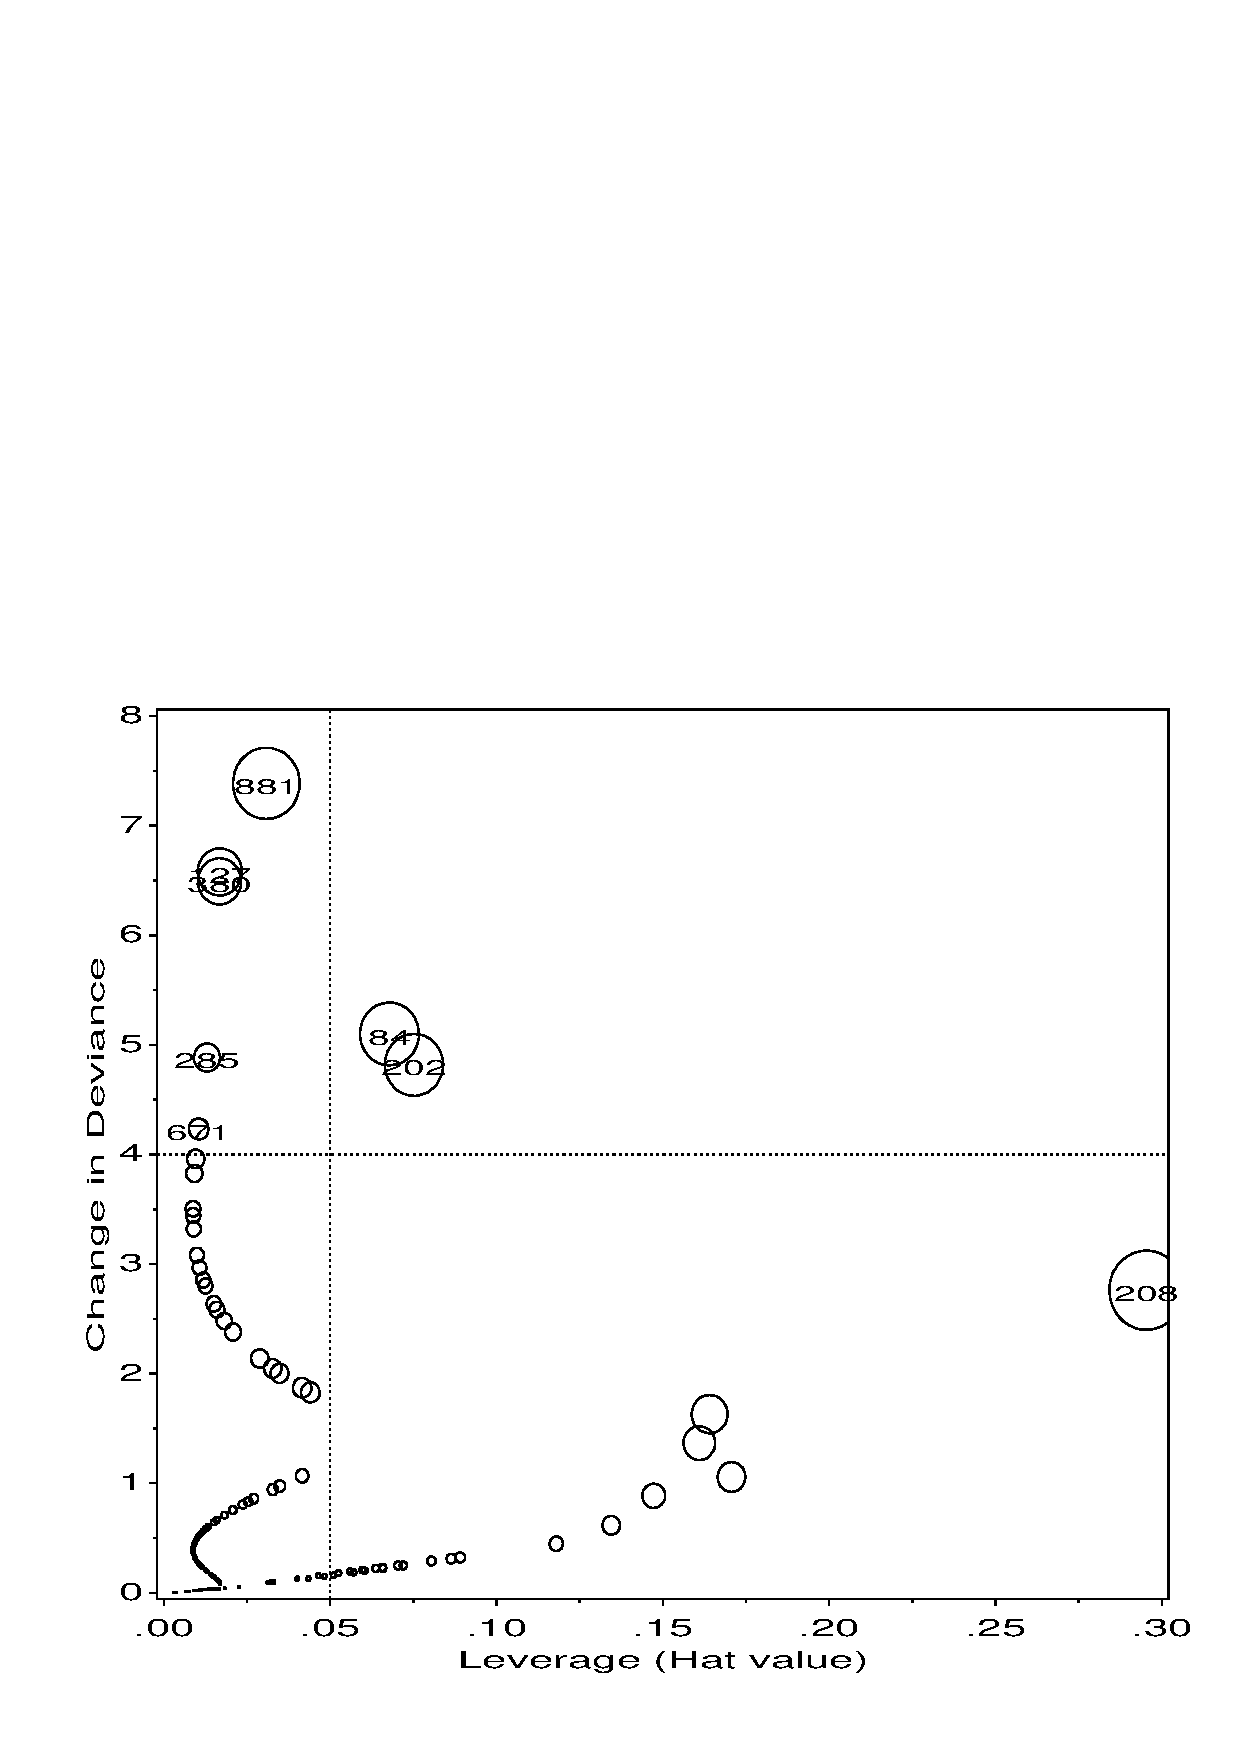
\includegraphics[scale=.6]{ch6/fig/icu12}
  \caption[ICU Survival data: Influence plot]{ICU Survival data: Influence plot}%
  \label{fig:icu12}
\end{figure}

Details for the cases identified in the figure are shown in \outref{out:icu1.2}.
None of the cases are particularly influential on the model coefficients overall:
the largest $C_i$ is only 1.04.
Case 208, with the largest hat value, is unusual on the predictors
in this sample: a 70 year old man without cancer, admitted on an elective
basis (who nonetheless died).
On the other hand, case 881, an 89 year old male, admitted unconscious
as an emergency case is poorly predicted because he survived.
Similarly, two other cases (127, 380) with large $\Delta \chi_{(-i)}^2$
are poorly predicted because they died, although they were
young, did not have cancer, and conscious at admission.
From this evidence we might conclude that none of these cases greatly affects the model, its coefficients,
or interpretation.
\begin{Output}[htb]
\caption{ICU data: Influential cases}\label{out:icu1.2}
\small
\verbatiminput{ch6/out/icu1.2}
\end{Output}

That conclusion might not be warranted without further study, particularly
in terms of influence on individual coefficients.
The DFBETAs \eqref{eq:dfbeta} may be obtained in an \ODS\ as shown below:
\begin{listing}
proc logistic data=icu;
   model died = age admit cancer uncons;
   output out=stats dfbetas=dbint dbage dbadmit dbcancer dbuncons ;
\end{listing}

%% two subfig side-by-side
\begin{figure}[htb]
 \begin{minipage}[t]{.49\linewidth}
  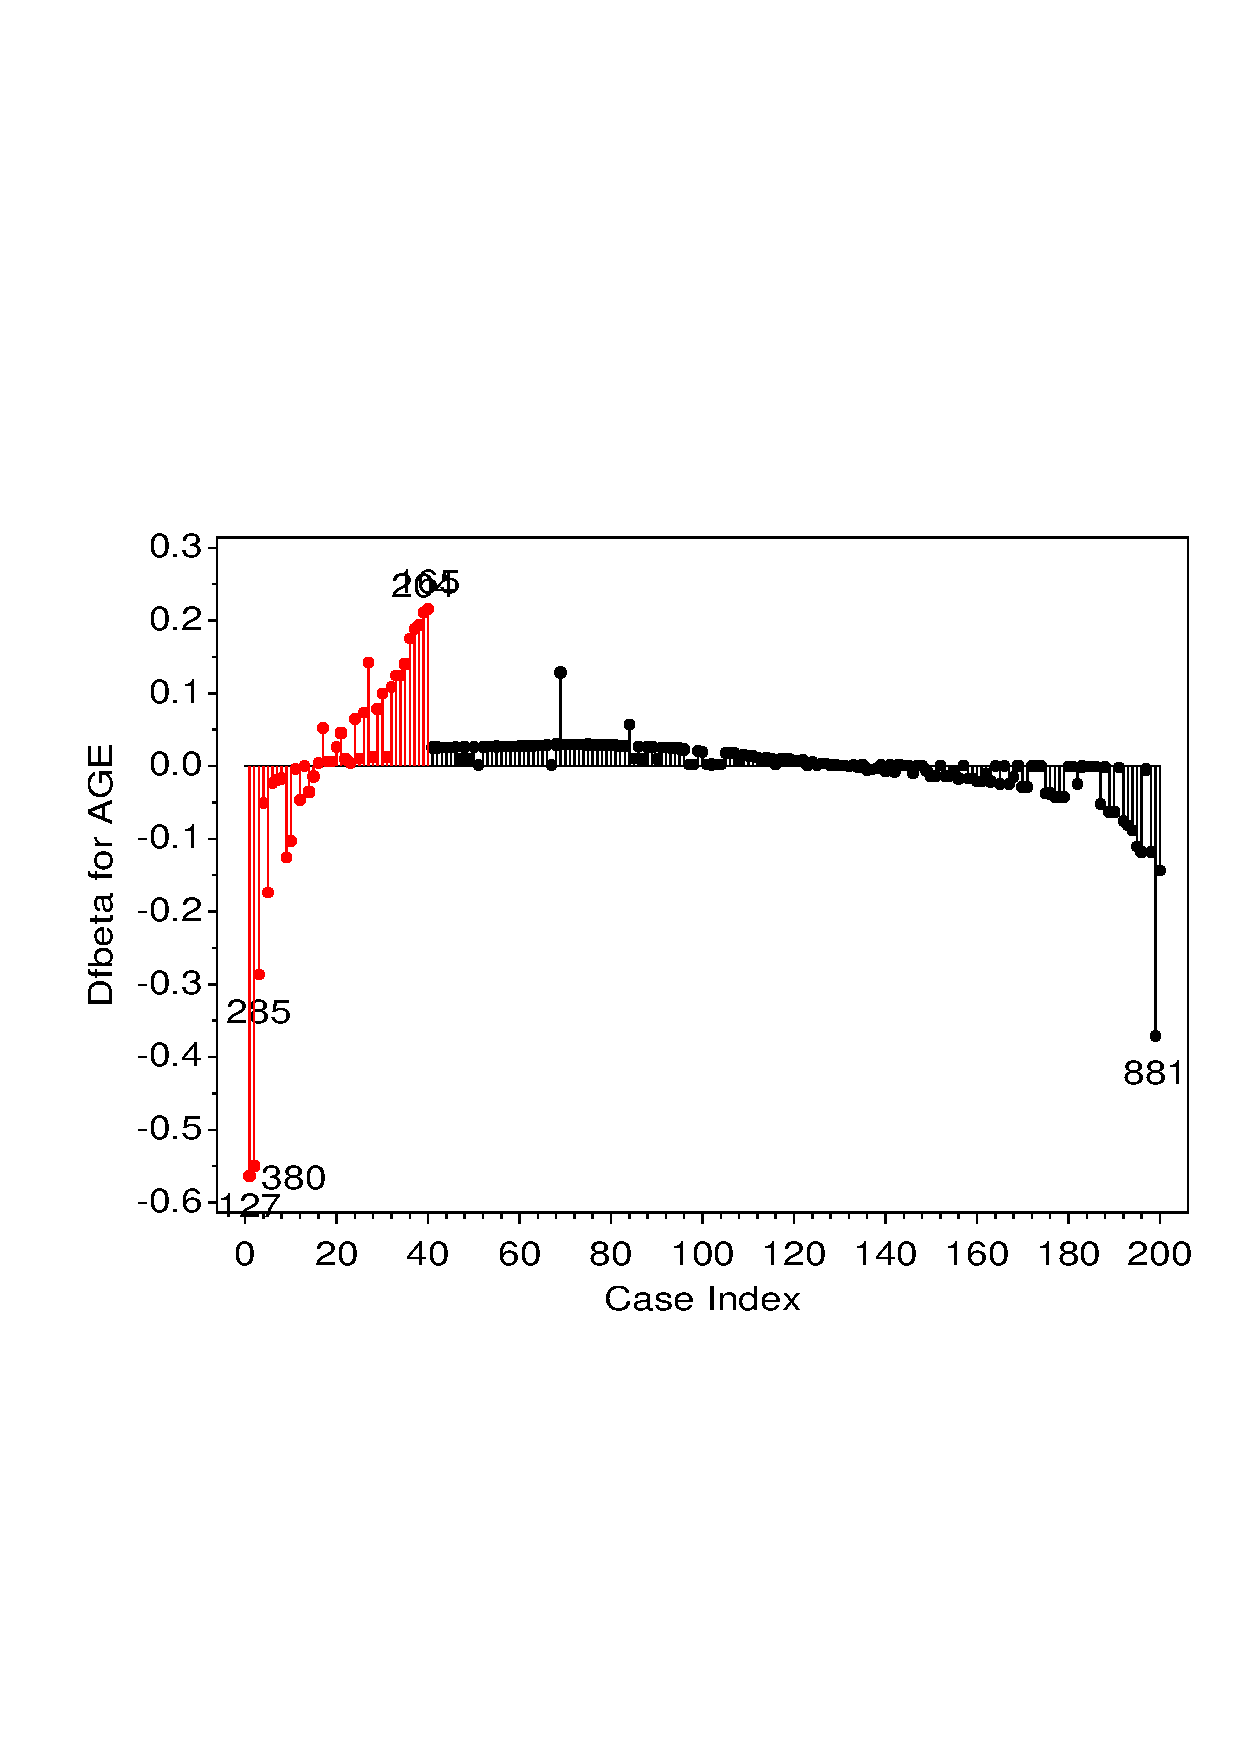
\includegraphics[width=1\linewidth,clip]{ch6/fig/icu4b1}
 \end{minipage}%
 \hfill
 \begin{minipage}[t]{.49\linewidth}
  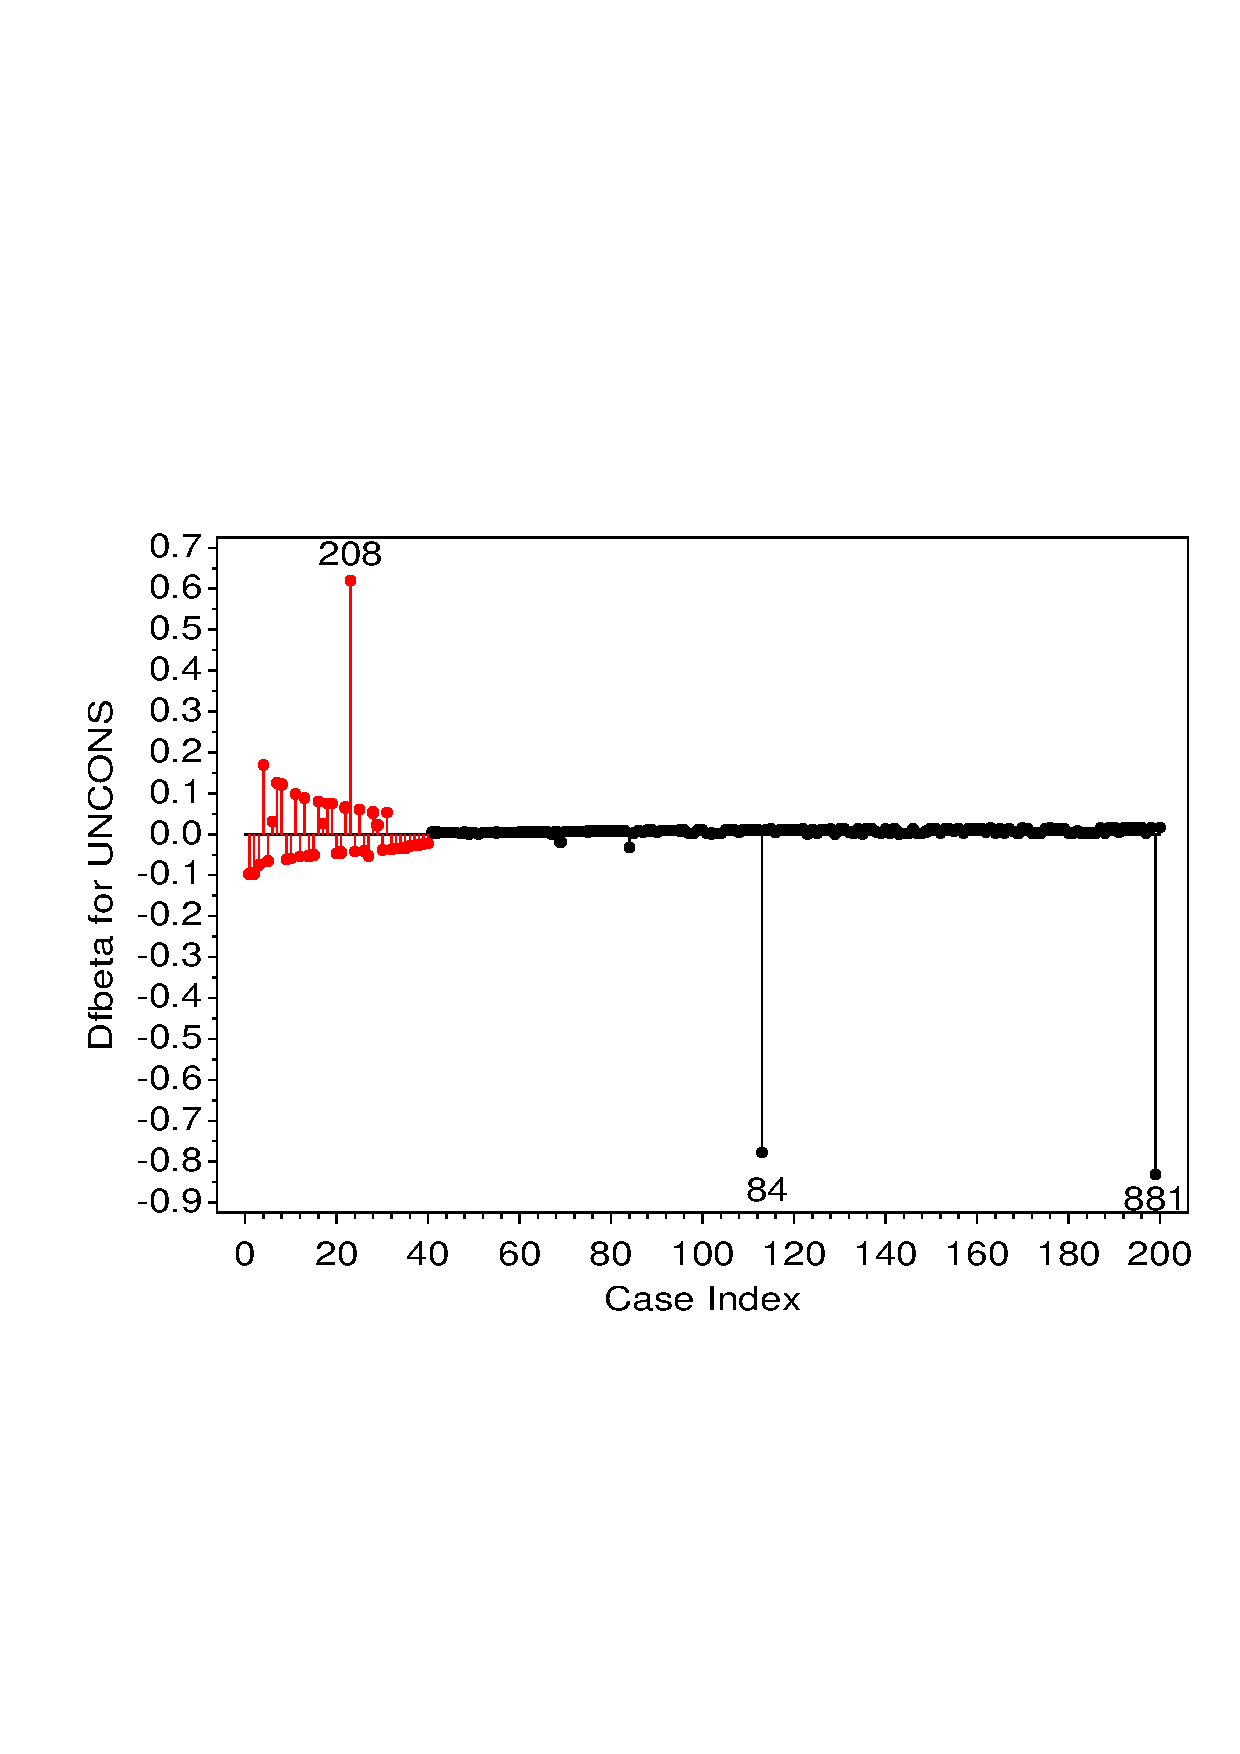
\includegraphics[width=1\linewidth,clip]{ch6/fig/icu4b2}
 \end{minipage}
 \caption{ICU data: DFBETA index plots for Age and Uncons}\label{fig:icu4b}
\end{figure}
Individual DFBETAs are often graphed as \emph{index plots}, that is,
for variable $j$ a plot of DFBETA$(i, j)$ against the case index $i$.
In such plots, it is helpful to label points with large absolute
values when (as here) the case number is not meaningful.
For example, the following statements produce an index plot of the
DFBETA for age, shown in \figref{fig:icu4b}.
The \macro{LABEL} is used to label points by the patient \pname{id},
where the DFBETA value exceeds 0.2 (an arbitrary value) in magnitude.
\begin{listing}
data stats;
   set stats;
   case = _n_;

%label(data=stats, x=case, y=dbage, text=put(id,3.), pos=-,
    subset=abs(dbage)>.2, out=labs);

proc gplot data=stats;
   plot dbage * case = died /
      anno=labs frame nolegend vaxis=axis1 haxis=axis2 vm=1;
   symbol1 i=needle v=dot c=black;
   symbol2 i=needle v=dot c=red;
   axis1 label=(a=90) length=4.5in;
   axis2 offset=(2) ;
\end{listing}
An alternative display, which is often more informative (though possibly more complex) is a scatterplot matrix of the DFBETAs, perhaps with other
influence diagnostics as well.
The pairwise scatterplots help to highlight observations which are
influential on both or only one of each pair of measures.
An example is shown in \figref{fig:icu4a}, produced with the
\macro{SCATMAT}:
\begin{listing}
%scatmat(data=stats,
   var= dbAge dbAdmit dbCancer dbUncons, group=died,
   symbols=star square,
   plotopt=%str(href=-0.2 0.2 vref=-0.2 0.2 cvref=graya0 chref=graya0));
\end{listing}

%% one figure
\begin{figure}[htb]
  \centering
  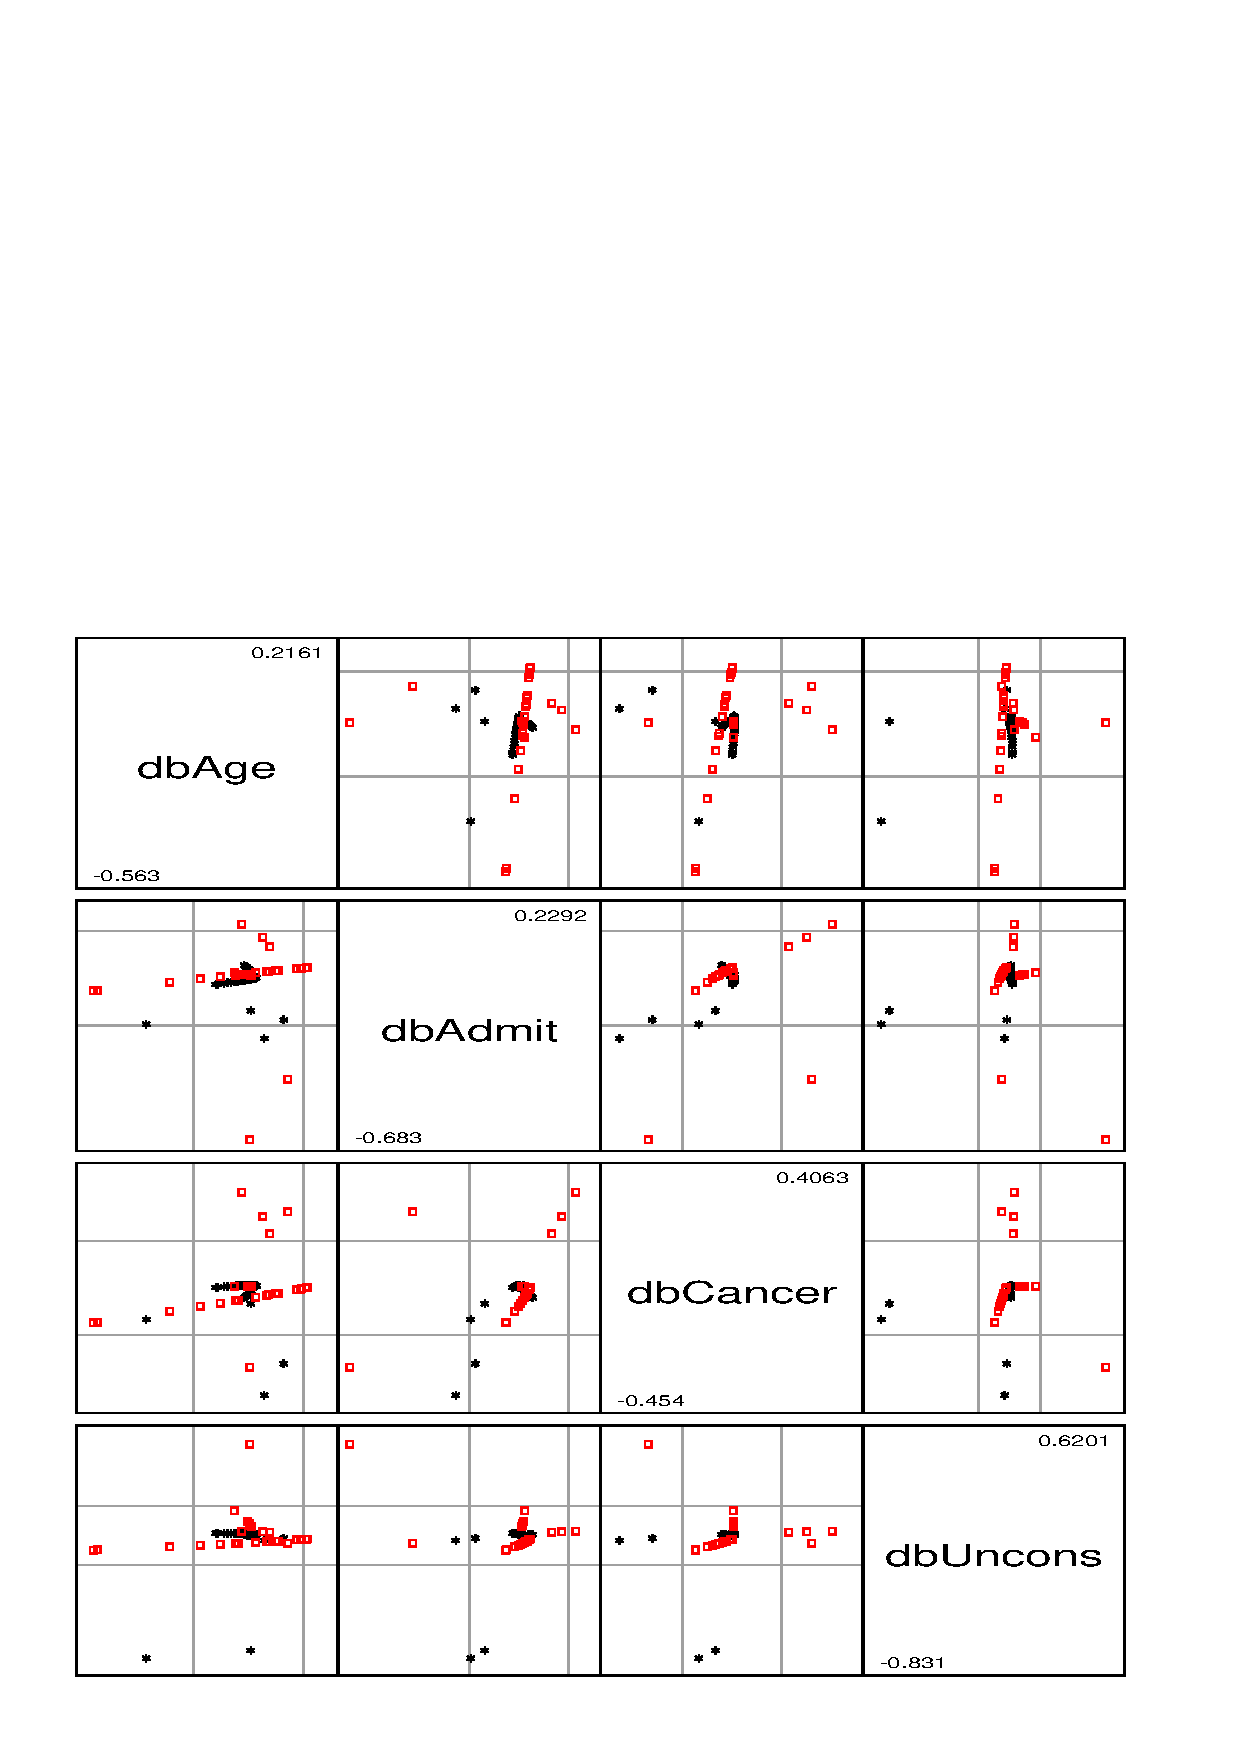
\includegraphics[scale=.75]{ch6/fig/icu4a}
  \caption[ICU Survival data: Scatterplot matrix of DFBETAs]{ICU Survival data: Scatterplot matrix of DFBETAs.  Those who lived are shown by $\star$s,  those who died are shown by squares.
  The reference lines indicate values of $\pm 0.2$ on each statistic.}%
  \label{fig:icu4a}
\end{figure}
Most of the observations are in the central rectangle, corresponding to
small values ($< \pm 0.2$) on both measures, but several points stand out
on the pairwise combinations.  For example, the bottom row and
rightmost column (DFBETA for \pname{UNCONS})
highlight two observations for patients who lived ($\star$s)
whose omission would decrease the coefficient for \pname{UNCONS}
considerably, and one who died whose omission would increase it.
Other observations outside the central rectangle might also be investigated.
\end{Example}

\subsection{Partial residual and added-variable plots}\label{sec:logist-partial}
The graphical methods described in this section are relatively
straight-forward indicators of the adequacy of a particular model,
with a specified set of predictors, each expressed in a given way.
More sophisticated methods have also been proposed, which focus on the need to include a particular predictor and whether its relationship is linear.
These include the \glossterm{partial residual plot},
\glossterm{added-variable plot}, and the
\glossterm{constructed variable plot},
which are all analogous to techniques developed in OLS.

\subsubsection{Partial residual plots}
The partial residual plot \citep{LarsenMcCleary:72} is designed to
show whether a given variable, $x_j$, included linearly in the model,
actually shows a nonlinear relation, requiring transformation.
As adapted to logistic regression by \citet{Landwehr-etal:84},
the partial residual for variable $x_j$ is defined as
\begin{equation*}%\label{eq:partres}
\vec{r}^{\star} = \mat{V}^{-1} \vec{r} + \beta_j \vec{x}_j
 = \frac{\vec{y} - \vec{p}}{ \vec{p} (1 - \vec{p})} \period
\end{equation*}
The partial residual plot is then a plot of $\vec{r}^{\star}$ against
$\vec{x}_j$, possibly with the addition of a smoothed lowess curve
\citep{Fowlkes:87} and
a linear regression line to aid interpretation.
If $x_j$ affects the binary response linearly, the plot should be approximately linear with a slope approximately equal to $\beta_j$.
A nonlinear plot suggests that $x_j$ needs to be transformed, and
the shape of the relation gives a rough guide to the required
transformation.
For example, a parabolic shape would suggest a term in $x_j^2$.

\subsubsection{Added variable plots}
The added variable plot, developed for generalized linear models by
\citet{WangP:85}, is a diagnostic plot designed to indicate whether
some new regressor, $z$, should be added to the model
which includes other explanatory variables.
An overall test could be based on the difference in $G^2$ for
the enlarged model $\logit(\vec{p}) = \mat{X} \vec{\beta} + \gamma \vec{z}$,
compared to the reduced model
$\logit(\vec{p}) = \mat{X} \vec{\beta}$.
But the added variable plot shows whether the evidence for including
$z$ is spread throughout the sample or confined to a small subset
of observations.
The regressor $z$ may be a new explanatory variable, or a higher power
of a variable already in the model.

The added variable plot may be constructed by following the logistic
regression for the reduced model with the variables in $\mat{X}$
with one weighted least squares regression of $\vec{z}$ on
$\mat{X}$ to find the residual part, $z^{\star}$,  of $z$ not predicted
by the previous regressors.
Let $\vec{r}$ be the vector of Pearson residuals from the initial logistic
fit of $\vec{y}$ on the variables in $\mat{X}$,
and let $\mat{H}$ and $\mat{V} = \diag [ \hat{\vec{p}} ( 1 - \hat{\vec{p}})]$
be the hat matrix and V matrix from this analysis.
Then, the added variable plot is a \scat\ of
the residuals $\vec{r}$ against the $z$-residuals,
\begin{equation*}%\label{eq:addvar}
 \vec{z}^{\star} = ( \mat{I} - \mat{H} ) \mat{V}^{1/2} \vec{z} \period
\end{equation*}
The $z$-residuals are easily calculated as
$z_i^{\star} = ( z_i - \hat{z}_i ) \sqrt{v_{ii}}$,
where $\hat{z}_i$ is the fitted value of $z_i$
in a weighted least squares regression of $\vec{z}$ on $\mat{X}$
using the $v_{ii}$ as weights.

A linear relation in this plot indicates that $z$ should be included in the
model, but observations with extreme $z$-residuals would be highly
influential in this decision.  A line fitted to this plot should have
an intercept approximately zero, and a slope approximating the coefficient
$\gamma$ of $z$ in the full model.
Added variable plots are produced by the \macro{ADDVAR}, described
in \macref{mac:addvar} and illustrated in the following example.

\begin{Example}[icu3]{Survival in the ICU}
In \exref{ex:icu1} we saw that the backward selection method nominated
three other variables, Systolic, pH, and PCO in addition to the four
variables we have been using throughout.
Here we first investigate whether systolic (blood pressure) should be
added to the model which includes Age, Admit, Cancer and Uncons.

The \macro{ADDVAR} is called as follows, to produce \figref{fig:icu61}.
There is no evidence of a strong linear relation, suggesting that
Systolic blood pressure has only a weak relationship to the residual in the current model.  The smooth lowess curve suggests
that any relationship may
be mildly quadratic
(though partial residual plots are generally preferable for detecting
nonlinearity).
The labeled points are those whose studentized Pearson residuals
exceed 2 in absolute value.
\begin{listing}
%addvar(data=icu,
   y=Died,                       /* response */
   x=age admit cancer uncons,    /* original predictors */
   z=Systolic,                   /* added variable */
   id=patient,                   /* id variable */
   smooth=0.5);                  /* lowess smoothing fraction */
\end{listing}

\begin{figure}[htb]
  \centering
  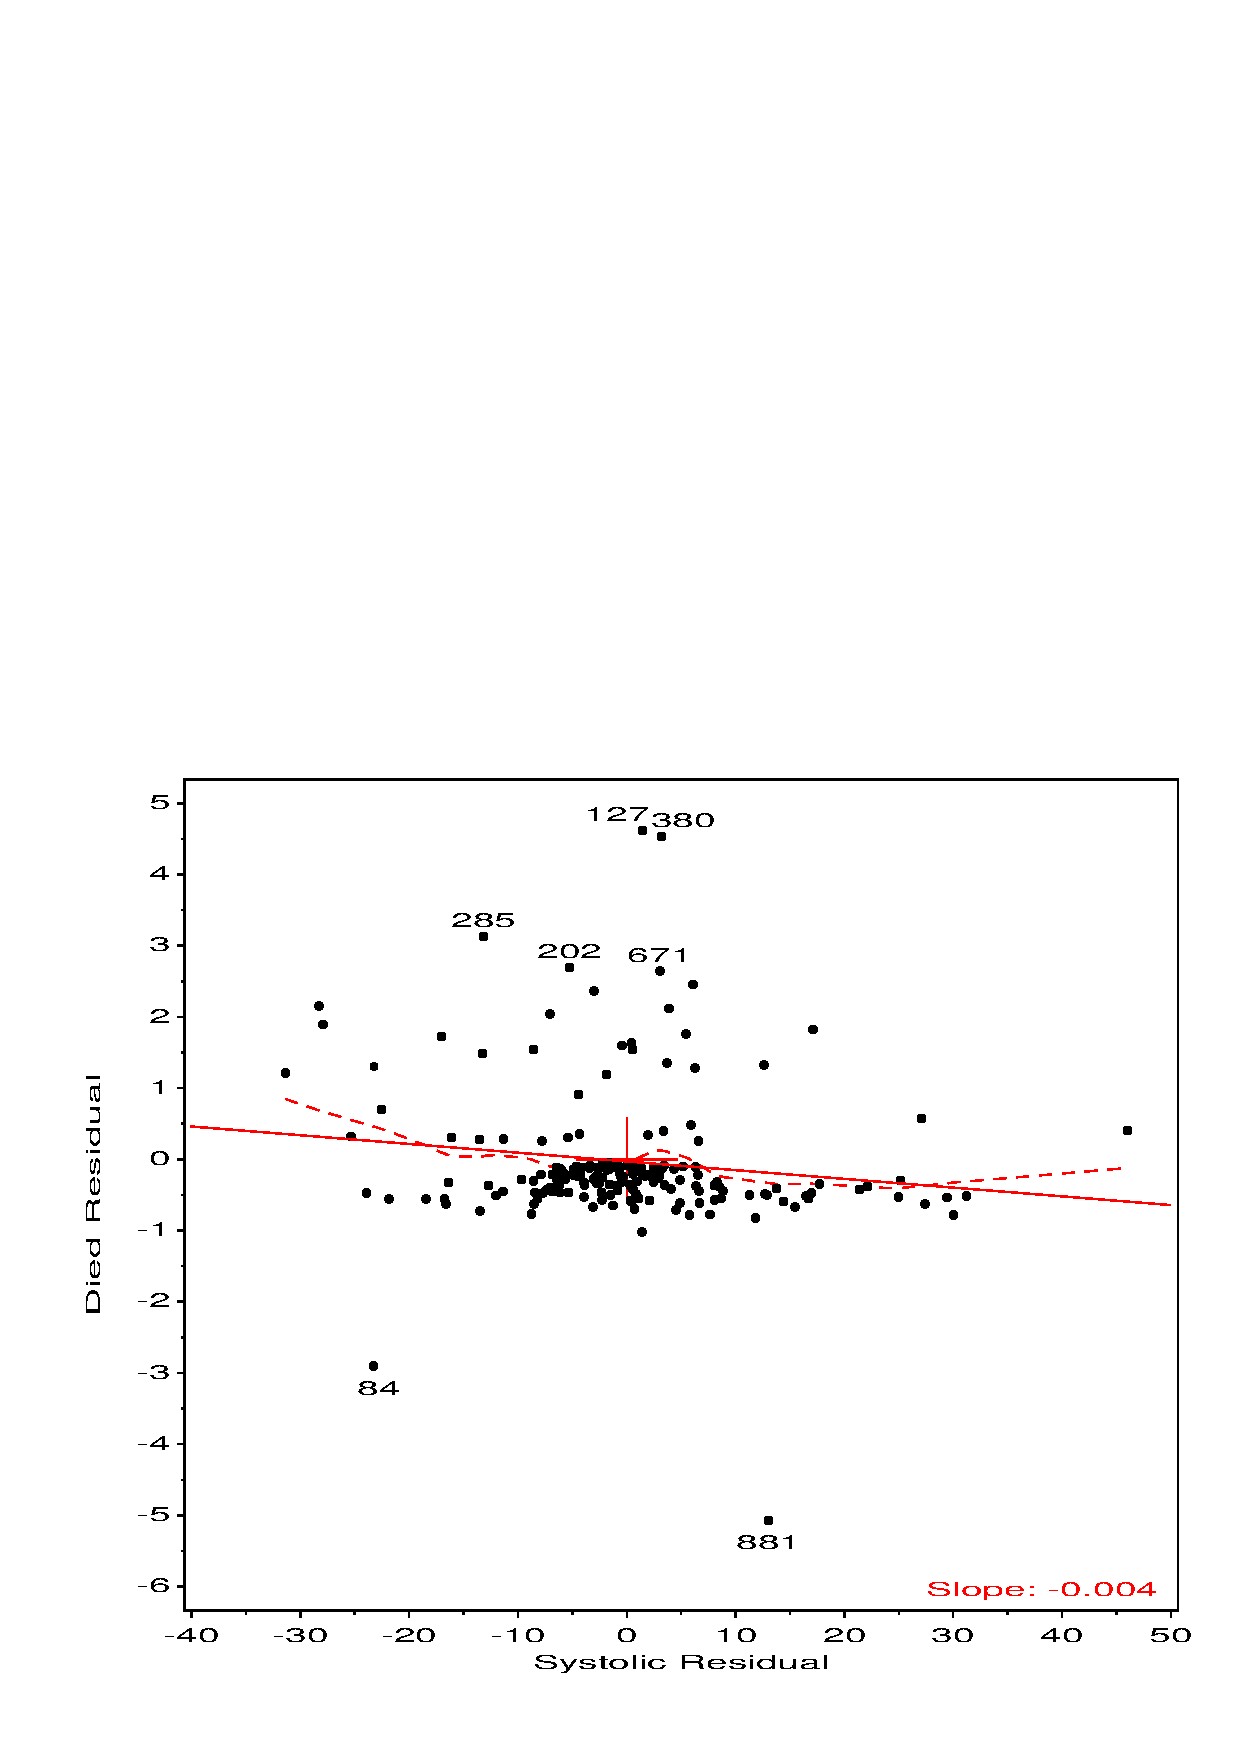
\includegraphics[scale=.6]{ch6/fig/icu61}
  \caption[ICU data: Added variable plot for Systolic blood pressure]{ICU data: Added variable plot for Systolic blood pressure.
 The solid line shows the weighted least squares regression of residuals
 on the Systolic residuals.  The broken curve is the lowess smooth.}%
  \label{fig:icu61}
\end{figure}

The added variable plot may also be used to determine if a regressor
should be included with an additional polynomial term.
For example we might check to see if Age${}^2$ should be included
in the model.  The statements below produce \figref{fig:icu62}.
\begin{listing}
data icu;
   set icu;
   age2 = .01 * (age-57.5)**2;

%addvar(data=icu, y=Died,  x=age admit cancer uncons, z=Age2,
   id=patient, smooth=0);
\end{listing}

%% one figure
\begin{figure}[htb]
  \centering
  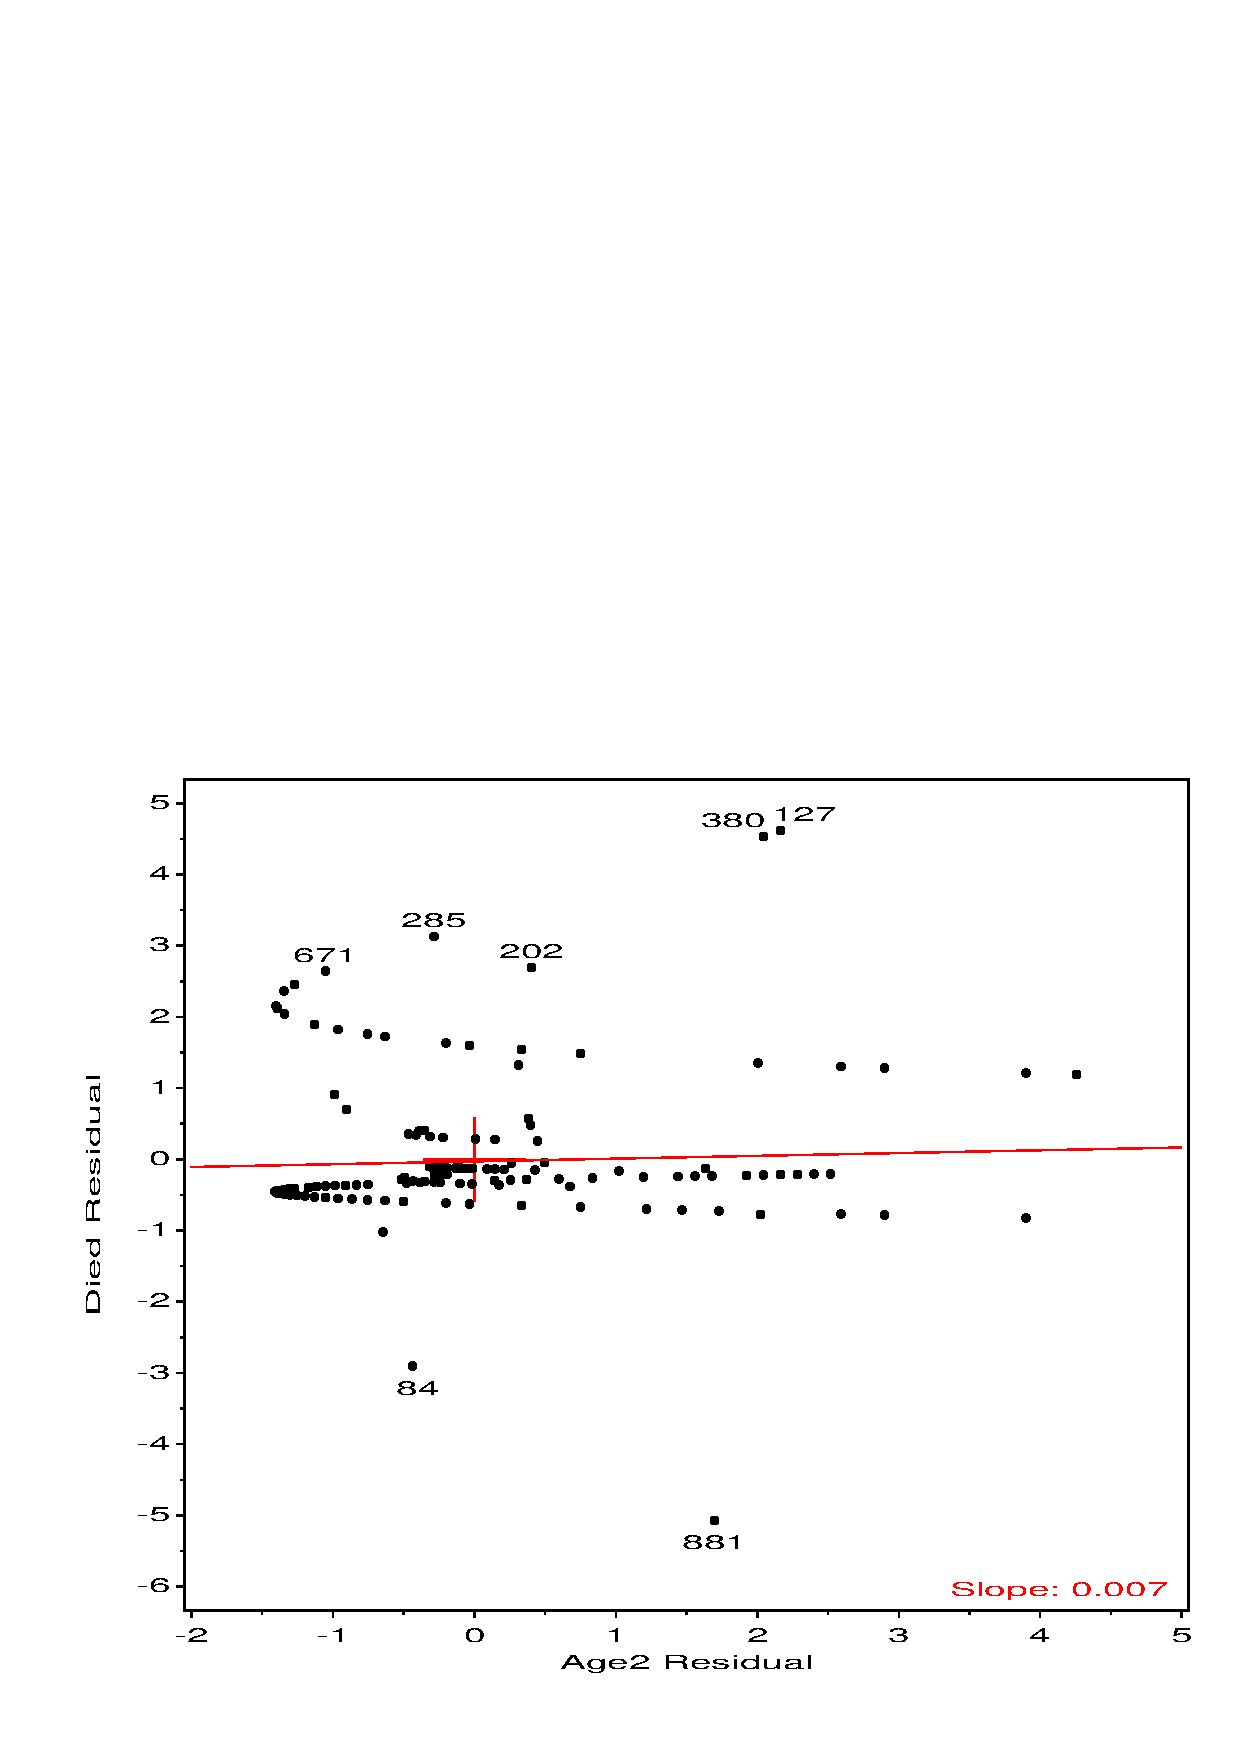
\includegraphics[scale=.6]{ch6/fig/icu62}
  \caption{ICU data: Added variable plot for Age${}^2$}%
  \label{fig:icu62}
\end{figure}
The slope of the line in \figref{fig:icu62} is approximately zero,
so we conclue that the squared term in Age is unnecessary.
\end{Example}

\subsubsection{Constructed variable plots}
While the partial residual plot is designed to detect a nonlinear relation
between the response and an explanatory variable,
it does not indicate the required transformation explicitly
and sometimes fails to diagnose nonlinearity
\citep{FienbergGong:84}.
The constructed variable plot, suggested for OLS regression
by \citet{Atkinson:81} and
\citet[\S 2.4.4]{CookWeisberg:82}, is specifically designed to
detect nonlinear dependence \emph{and} to suggest a power transformation
of the explanatory variable which would make the relation linear.
This plot was extended to generalized linear models by
\citet{WangP:87}.

Suppose that the variable $x_j$ is included in the model, and we are
contemplating replacing $x_j$  by a power $x_j^{(\lambda)}$ , defined by
the family \citep{BoxCox:64}
\begin{equation}\label{eq:boxcox}
x ^{(\lambda)} = \left\{
\begin{array}{cl}
\frac{x^\lambda - 1}{\lambda}, & \lambda \ne 0 \\
\log (x),  & \lambda = 0 \\
\end{array}
\right. \period
\end{equation}
To determine if a transformation is necessary, the constructed variable,
$z_j = b_j x_j \log x_j$ is calculated, where
$b_j$ is the estimated coefficient for $x_j$ in the original model.
Then the constructed variable plot is just an added variable plot for
$z_j$.

A linear trend, with a non-zero slope $\gamma$, in the constructed variable
plot indicates that a transformation of $x_j$ is necessary,
and the estimate of the power transformation in \eqref{eq:boxcox} is
$\hat{\lambda} = 1 + \gamma$, usually rounded to the nearest half-integer.
The absence of a linear trend means that $x_j$ is linear in the model.



\section{Polytomous response models}\label{sec:logist-poly}

When the response, $y$, takes on $m > 2$ discrete values, there are
several ways to model the response probabilities.  Let \(\pi_{ij} \equiv
\pi_j \,  ( \vec{x}_i )\) be the probability of response j for case
or group i, given the predictors $\vec{x}_i$.
Because \(\sum_j \,  \pi_{ij} = 1\), only \(m - 1\) of
these probabilities are independent.

The simplest approach uses
the 
\glossterm{proportional odds model}, described in \secref{sec:ordinal}.
This model applies only when the response is ordinal,
\emph{and} an additional assumption
(the proportional odds assumption) holds.  
However, if the
response is purely nominal (e.g., vote Tory, Liberal, Reform, NDP),
or if the proportional odds assumption is untenable, another particularly
simple strategy is to fit separate models to a set of \(m - 1\)
\glossterm{nested dichotomies} derived from the polytomous response
(\secref{sec:nested}).
Both of these methods are handled by \PROC{LOGISTIC}.

A third strategy, described in \secref{sec:genlogit}, is to choose one
    response category (the last, say) as the ``base category'', and
    model the \glossterm{generalized logits} for each of categories
    \(j = 1, 2, \dots , (m - 1)\) compared to category m.  For a
    3-category response, e.g., there are 2 generalized logits,
     \(\logit_{i1}  = \log  ( { \pi_{i1} } /  { \pi_{i3} })\) and
     \(\logit_{i1}  = \log  ( { \pi_{i2} } /  { \pi_{i3} })\).
     These models can be fit using \PROC{CATMOD}.

\section{Models for ordinal variables}\label{sec:loglin-ordinal}
Standard \loglin\ models treat all classification variables as
nominal, unordered factors;
all statistical tests are identical
and parameter estimates are equivalent
if the categories of any variable are reordered.
Yet we have seen that the ordering of categories often provides
important information about the nature of associations
and we showed (\secref{sec:ordinaltests}) that non-parametric
tests which take into account the ordered nature of a factor
are more powerful.

In a mosaic display, an ordered associative effect is seen when
the residuals have an opposite-corner pattern of positive and negative
signs and magnitudes (e.g., for the hair-eye color data,
\figref{fig:mosaic34} or the Titanic data, \figref{fig:mostitanic1}).
In a correspondence analysis plot,
an association has an ordered effect when the points for two factors are
ordered similarly.
In these cases \loglin\ and logit models which use the ordered nature of the factors
offer several advantages.
\begin{itemize}
\item Because they are more focused, tests which use the ordinal
structure of the table variables are more powerful when the association
varies systematically with the ordered values of a factor.

\item Because they consume fewer degrees of freedom,
we can fit unsaturated models where the corresponding model for
nominal factors would be saturated.
In a two-way table, for example, a variety of models for ordinal
factors may be proposed which are intermediate between the independence
model and the saturated model.

\item Parameter estimates from these models are fewer in number, and are
easier to interpret, and quantify the nature of effects better
than corresponding quantities in models for nominal factors.
Estimating fewer parameters typically gives smaller standard errors,
as we saw in \exref{ex:reagan}.
\end{itemize}
These advantages are analogous to the use of tests for trends or
polynomial effects in ANOVA models.

Models for ordinal variables may be specified in \loglin\ form,
as described in \secref{sec:loglin-ordlog}.  When there is an ordinal
response variable, related models may be specified in terms of
logits for adjacent categories (\secref{sec:loglin-ordadj}),
or cumulative logits (\secref{sec:loglin-ordcum}).
The descriptions here are brief. For further information refer to
\citet{Agresti:84}, \citet[Ch. 9]{Agresti:90} and
\citet{Goodman:79,Goodman:83}.

\subsection{Loglinear models for ordinal variables}\label{sec:loglin-ordlog}
For a two-way table, when either the row variable or the column variable,
or both, are ordinal, one simplification comes from assigning ordered
scores, $\{a_i\}, a_1 \le a_2 \le \cdots a_I$, and/or
$\{b_j\}, b_1 \le b_2 \le \cdots b_J$
to the categories
so that the ordinal relations are necessarily included in the model.
Typically, equally spaced scores are used, for example, integer
scores, $\{a_i\}=i$, or the zero-sum equivalent, $\{a_i\}=i-(I+1)/2$
(e.g., $\{a_i\}= \{-1, 0, 1\}$ for $I=3$).
These give simple interpretations of the
association parameters in terms of \emph{local odds ratios},
\begin{equation*}
 \theta_{ij} =
 \frac{ m_{ij} \: m_{i+1, j+1} } { m_{i,j+1} \: m_{i+1, j} }
 \comma
\end{equation*}
the odds ratio for adjacent rows and adjacent columns.

When both variables are assigned scores, we have the \glossterm{linear-by-linear model},
\begin{equation}\label{eq:linlin}
\log ( m_{ij} ) = \mu  +  \lambda_i^A
+  \lambda_j^B  +  \gamma \: a_i b_j \period
\end{equation}
Because the scores are fixed, this model has only one extra parameter, $\gamma$, compared to the
independence model, which is the special case, $\gamma=0$.
The terms  $\gamma a_i b_j $ describe a pattern of association
where deviations from independence increase linearly with $a_i$
and $b_j$ in opposite directions towards the opposite corners of
the table.

In the linear-by-linear association model, the local log odds ratios
are
\begin{equation*}
\log \theta_{ij} =
 \gamma (a_{i+1} - a_i) (b_{j+1} - b_j)
 \comma
\end{equation*}
which reduces to
\begin{equation*}
\log \theta_{ij} =
 \gamma
\end{equation*}
for integer-spaced scores, so $\gamma$ is the common local log odds ratio.
As a result, the linear-by-linear model is sometimes called the
model of \emph{uniform association} \citep{Goodman:79}.
\ix{uniform association model}
\ix{linear-by-linear model}
\ix{log odds ratio!local}

Generalizations of the linear-by-linear model result when only one
variable is assigned scores.
In the \glossterm{row-effects model},
the row variable, say, $A$ is treated as nominal, while
the column variable, $B$, is assigned ordered scores $\{b_j\}$.
The \loglin\ model is then
\begin{equation}\label{eq:roweff}
 \log ( m_{ij} ) = \mu  +  \lambda_i^A
  +  \lambda_j^B  +  \alpha_i b_j
 \comma
\end{equation}
where the $\alpha_i$ parameters are the \emph{row effects}.
An additional constraint,
$\sum_i \alpha_i =0$ or $\alpha_I =0$
 is imposed, so that model \eqref{eq:roweff}
has $(I-1)$ more parameters than the independence model.
The linear-by-linear model is the special case where the row effects
are equally spaced, and the independence model is the special case
where all $\alpha_i = 0$.

The row-effects model \eqref{eq:roweff} also has a simple odds ratio interpretation.
The local log odds ratio for adjacent pairs of rows and columns is
\begin{equation*}
\log \theta_{ij} =
  \alpha_{i+1} - \alpha_i
  \comma
\end{equation*}
which is constant for all pairs of adjacent columns.  Plots of the
local log odds ratio against $i$ would appear as a set of parallel
curves.

In the analogous \glossterm{column-effects model}, $(J-1)$ linearly independent
column effect
parameters $\beta_j$ are estimated for the column variable, while fixed
scores $\{a_i\}$ are assigned to the row variable.

The linear-by-linear model \eqref{eq:linlin} and the row-effects model
\eqref{eq:roweff} can be fit using \PROC{CATMOD},
but to do so requires that you enter the complete model matrix explicitly.
With \PROC{GENMOD} you need only create a numeric variable with score
values in the input \Dset, a much easier task.
\begin{Example}[mental2]{Mental impairment and parents' SES}
In \exref{ex:mental1} \CA\ was used to explore the relationship between
ratings of the mental health status of young New Yorkers and
their parents' socioeconomic status (SES).
\figref{fig:correses} showed that most of the association in the
table was accounted for by a single dimension along which both factors
were ordered, consistent with the view that mental health increased
in relation to parents' SES.

For comparison, we first fit the independence model with both
\PROC{CATMOD} and \PROC{GENMOD}.
As we expect, this model fits quite badly,
with $\GSQ\ (15) = 47.418$.
\begin{listing}
%include catdata(mental);
proc catmod data=mental;
   weight count;
   model mental*ses = _response_ / noiter noprofile noresponse;
   loglin mental ses / title='Independence';
   run;
\end{listing}
For illustration, the standardized (adjusted) deviance residuals,
$g_i / \sqrt ( 1 - h_i )$
are obtained in the \PROC{GENMOD}
step (named \pname{stresdev} in the \pname{obstats} \Dset),
and used with the \macro{MOSAIC} to produce the mosaic
display shown in the left panel of \figref{fig:mental2}.%
\footnote{To ensure that the the levels of both factors are ordered
correctly, \pname{MENTAL} and \pname{SES} were entered as numeric
variables in the \Dset\ \pname{MENTAL}, and user-formats were used
to provide the character labels shown in \figref{fig:mental2}.
Because \IML\ does not make use of formatted values, the \macro{TABLE}
was used to convert the numeric variables to character.
}
The parameter \pname{cellfill=dev 0.5}
causes the program to write the value of all residuals greater than 0.5
in absolute value in the corresponding tile.
\begin{listing}
proc genmod data=mental;
   class mental ses;
   model count = mental ses / dist=poisson obstats residuals;
   make 'obstats' out=obstats noprint;
run;

%table(data=mental, var=Mental SES, weight=count, char=Y,
       format=mental mental. ses ses., order=data, out=mental2);
data obstats;
   merge mental2 obstats;
%mosaic(data=obstats, vorder=Mental SES, plots=2, split=H V, resid=stresdev,
   title=Mental Impairment and SES: Independence, cellfill=dev 0.5);
\end{listing}
%% two subfig side-by-side
\begin{figure}[htb]
 \begin{minipage}[t]{.49\linewidth}
  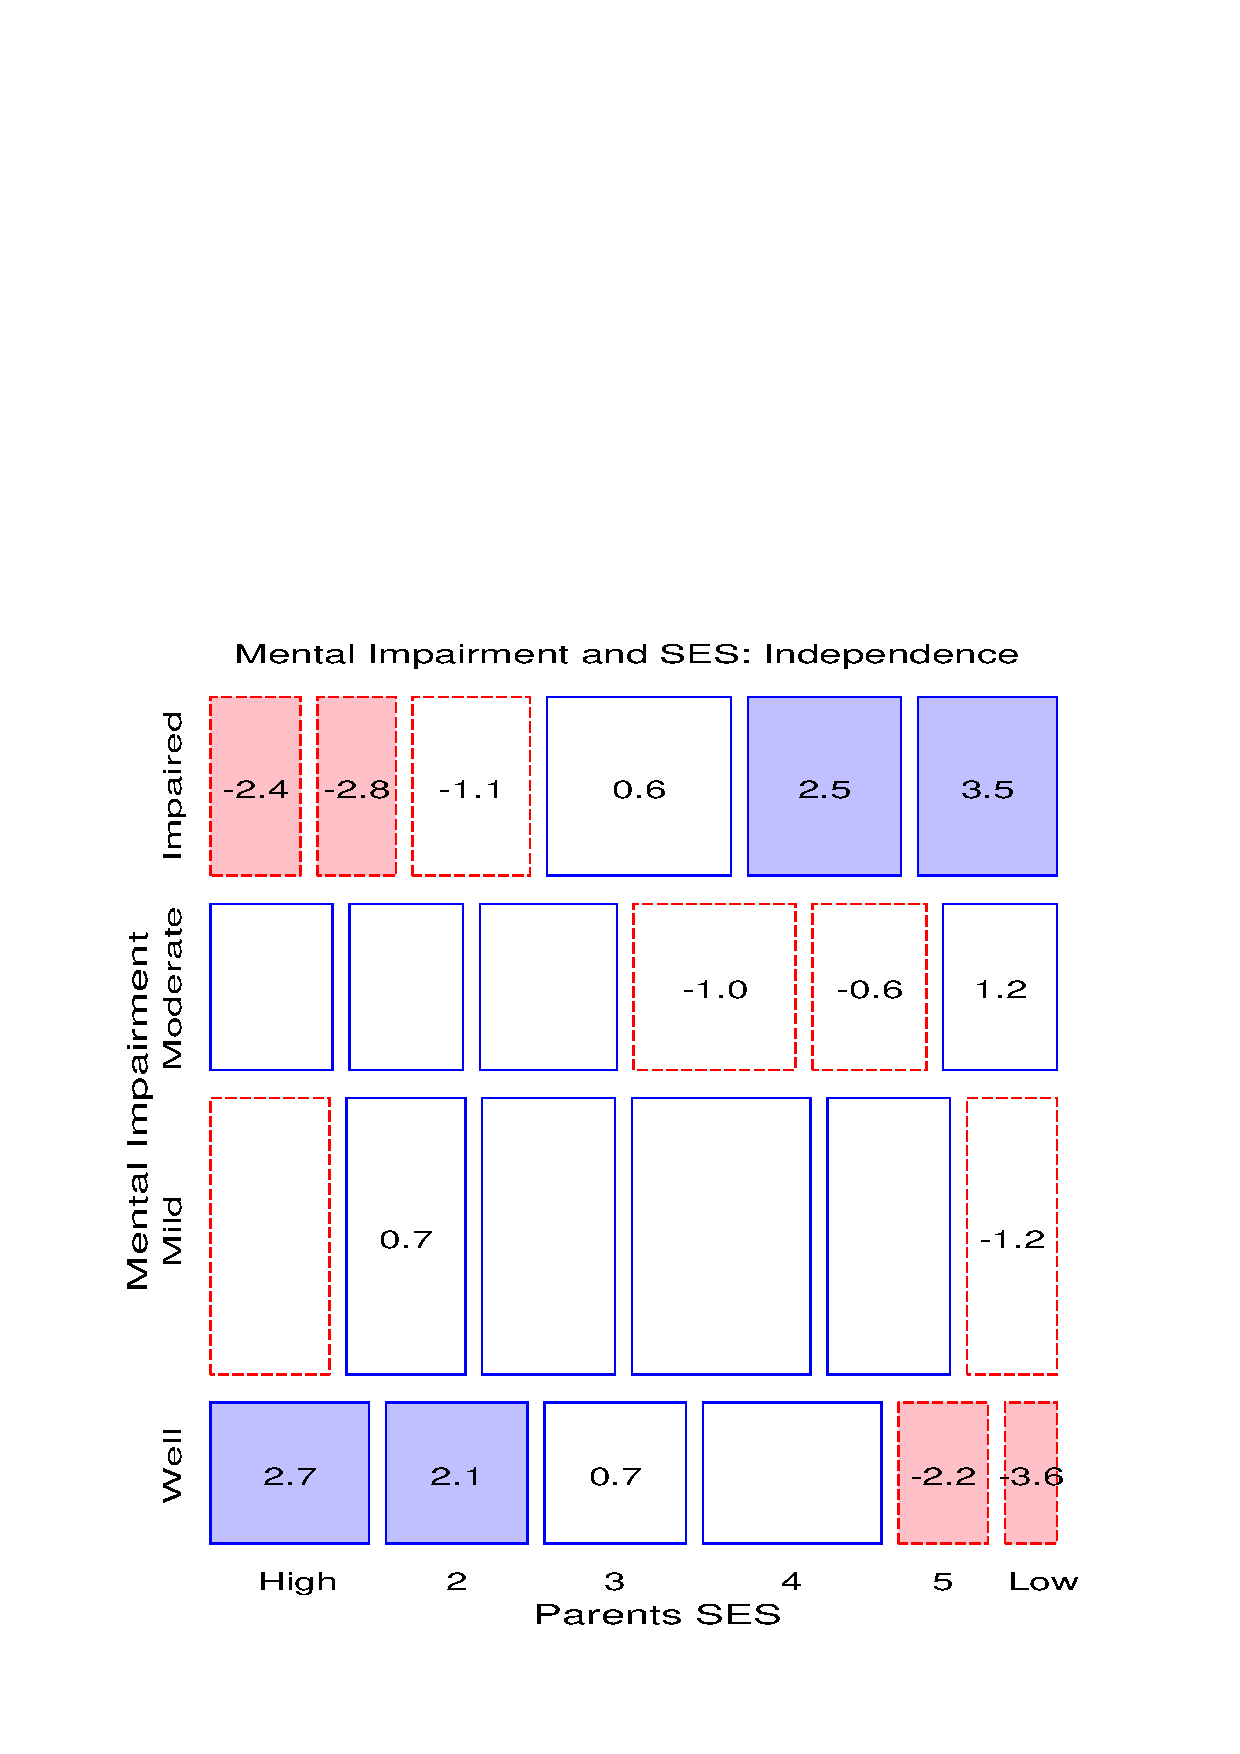
\includegraphics[width=1\linewidth]{mental21}
 \end{minipage}%
 \hfill
 \begin{minipage}[t]{.49\linewidth}
  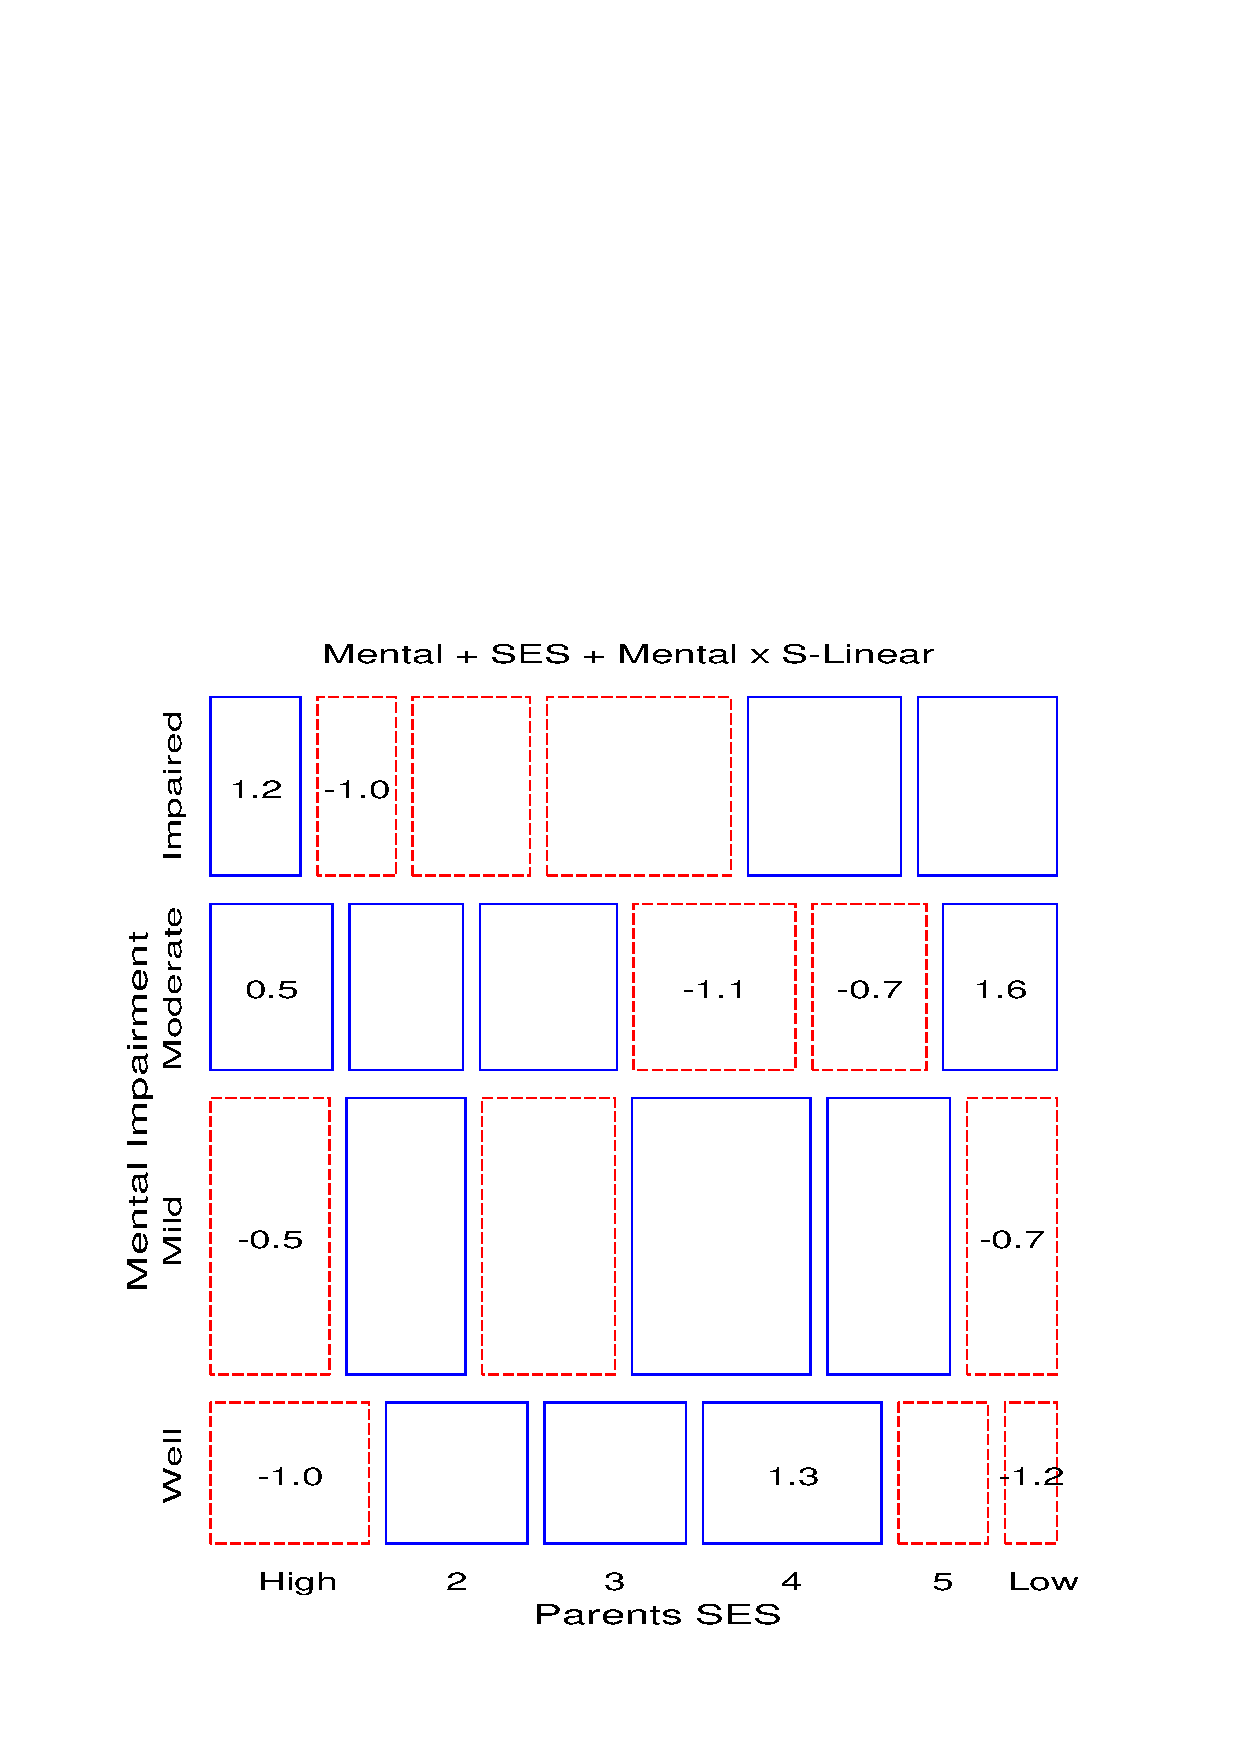
\includegraphics[width=1\linewidth]{mental22}
 \end{minipage}
 \caption[Mental health and SES: Residuals]{Mental health and SES: Residuals from Independence (left) and Row Effects (right) Models}\label{fig:mental2}
\end{figure}
Note that the residuals in \figref{fig:mental2} for the
independence model have the opposite-corner pattern which would
arise if either the row-effects model (with ordered row effects)
or the linear-by-linear
association model described the association between mental health
and SES.
\input{ch7/tab/mentab2}

To fit models in which the association terms for \pname{mental} and/or
\pname{ses} use quantitative scores, create copies, \pname{M} and
\pname{S} of these variables.  They are used as quantitative variables
when they appear in the \stmt{MODEL}{GENMOD}, but are \emph{not} listed
as \pname{CLASS} variables.
The following statements fit the row-effects model, using SES
as a linear effect, and then the linear-by-linear model.
Goodness-of-fit statistics for all three models are shown in
\tabref{tab:mentab2}.

\begin{listing}
data mental;
   set mental;
   m = mental;    *-- copy m and s as quantitative, non-class;
   s = ses;

title 'Linear SES';
proc genmod data=mental;
   class mental ses;
   model count = mental ses mental*s / dist=poisson obstats residuals;
   make 'obstats' out=obstats noprint;
run;
data obstats;
   merge mental obstats;
%mosaic(data=obstats, var=Mental SES, resid=stresdev,  split=H V,
   title=Mental + SES + Mental x S-Linear, cellfill=dev 0.5);

title 'Linear x Linear';
proc genmod data=mental;
   class mental ses;
   model count = mental ses m*s / dist=poisson obstats residuals;
run;
\end{listing}
The $\Delta \GSQ$ values in \tabref{tab:mentab2} each test whether
the corresponding model results in a significant reduction in the
residual $\GSQ$ compared to the independence model.  Both are
highly significant.

Similarly, the difference in $\GSQ$ between the linear-by-linear
and row-effects model, $\Delta \GSQ\ (2) = 9.732-6.289 = 3.443$ suggests that the 
row-effects model
is \emph{not} a significant improvement over the
linear-by-linear model.
The AIC values suggest a slight preference for the linear-by-linear model.
The residuals for the row effects model are shown in the right
panel of \figref{fig:mental2}; residuals for the linear-by-linear
model (not shown) have the same signs, but are slightly smaller
in some cells.

\begin{Output}[htb]
\caption{Parameter estimates for the row-effects \loglin\ model, Mental health data}\label{out:mental2.1}
\small
\verbatiminput{ch7/out/mental2.1}
\end{Output}

Under the linear-by-linear model, the estimate of the coefficient of
\pname{M*S} is $\hat{\gamma} = 0.0907$ (s.e.=0.015) with unit-spaced scores.
This corresponds to a local odds ratio, $\hat{\theta}_{ij} = \exp (0.0907) = 1.095$.
This single number describes the association succinctly:
each step down socioeconomic scale increases the odds of being classified
one step poorer in mental health by 9.5\%.

Parameter estimates for the row-effects model are shown in
\outref{out:mental2.1}.  The row effects are the values of
the \pname{S*MENTAL} terms.  These values are ordered, consistent with
mental health status having ordinal associative effects,
but (with integer scores for both variables) they are not equally
spaced, as the linear-by-linear model would imply.
The spacing of these parameter estimates is similar to what we saw
in the \CA\ plot (\figref{fig:correses}), with the middle categories
Mild Impairment, and Moderate Impairment relatively close together
compared to the extreme categories.

These \loglin\ models and the associated mosaic displays do not
provide a clear preference between the row-effects and linear-by-linear
models here.
We turn now to other models and graphical displays which may distinguish them better.
\end{Example}


\subsection{Adjacent category logit models}\label{sec:loglin-ordadj}
When there is a single response variable, logit models provide a
simple way to model the dependence of the response on the other,
explanatory variables.  For an ordinal response,
models for the logits between adjacent response categories
allow the ordered nature of the response to be taken into account.
For the model of independence, the \emph{adjacent category logits} are
\begin{eqnarray}
A_{j| i} \equiv
\log \left(
 \frac{ \pi_{j+1|i} } { \pi_{j|i} }
 \right) =
\log \left(
 \frac{ m_{i, j+1} } { m_{ij} }
 \right)
  & = &
( \mu  +  \lambda_i^A +  \lambda_{j+1}^B ) -
( \mu  +  \lambda_i^A +  \lambda_j^B )  \nonumber \\
  & = &  \lambda_{j+1}^B -  \lambda_{j}^B \label{eq:aindep}
\end{eqnarray}
which are constants, say, $\beta_j = (\lambda_{j+1}^B -  \lambda_{j}^B )$
not depending on the explanatory variable(s).
If an explanatory variable is also ordinal, we may use scores, $\{a_i\}$
as before.
The analog of the linear-by-linear model with unit-spaced scores
allows the value of $A_{j| i}$ to vary linearly with the quantitative value,
\begin{equation}\label{eq:alin}
A_{j| i} = \beta_j + \gamma \: a_i
\end{equation}
The slope parameter $\gamma$ has a similar log odds interpretation:
the log odds of a response in category $j+1$
as opposed to category $j$ increases by $\gamma$
for each unit increase in the explanatory variable.
% The intercept parameters, $\beta_j$ ...

In a similar way, the fixed scores $a_i$ may be replaced by row effect
parameters, $\alpha_i$ to be estimated (with the constraint $\sum_i \alpha_i =0$ or $\alpha_I =0$)
to give the row-effects adjacent logit model
\begin{equation}\label{eq:arow}
A_{j| i} = \beta_j + \alpha_i
\end{equation}
A plot of the fitted logits against $i$ for this model appears as parallel
curves (rather than parallel lines under the linear-by-linear model
\eqref{eq:alin}).

Even less restrictive models, which are still unsaturated, may be fit if the row-effects model fits poorly.  For example, each adjacent logit may be
linearly related to an assigned score for an explanatory variable,
but the slopes may differ over the adjacent response categories
(the \emph{linear-interaction model}):
\begin{equation}\label{eq:alin-int}
A_{j| i} = \beta_j + \gamma_j \: s_i \period
\end{equation}
Alternatively, a quadratic relation between the
adjacent logits, $A_{j| i}$ and the scores,
$A_{j| i} = \beta_j + \gamma_1 \: a_i + \gamma_2 a_i^2$
may be fit.
These possibilities are illustrated below.

\begin{Example}[mental4]{Mental impairment and parents' SES}
We consider here adjacent category logit models for the Mental Health
data, treating \pname{MENTAL} as an ordinal response.
Adjacent logit models are easily fit with \PROC{CATMOD}
using the \pname{RESPONSE ALOGIT;} statement.
Differences among the logits for adjacent categories (the intercepts, $\beta_j$, in models \eqref{eq:alin} and \eqref{eq:arow}) are
specified by the \verb|_RESPONSE_| keyword in the
\stmt{MODEL}{CATMOD}.  Nominal explanatory variables are included
as main effects (and possibly, interactions) on the left-hand side
of the \stmt{MODEL}{CATMOD}.  An explanatory variable is treated
as quantitative when declared in a \stmt{DIRECT}{CATMOD}.

The following statements fit a series of adjacent category logit models
to the Mental Health data.  Model 0 has only a \verb|_RESPONSE_|
effect, and is analogous to the independence model.
In Model 1, the adjacent logits for mental impairment are affected
by SES, as a nominal variable.
Model 2 is the linear-by-linear model for adjacent logits, with
SES as a direct variable,
while Model 3 allows different slopes for each adjacent logit.
\input{ch7/sas/mental41}
%% two subfig side-by-side
\begin{figure}[htb]
 \begin{minipage}[t]{.49\linewidth}
  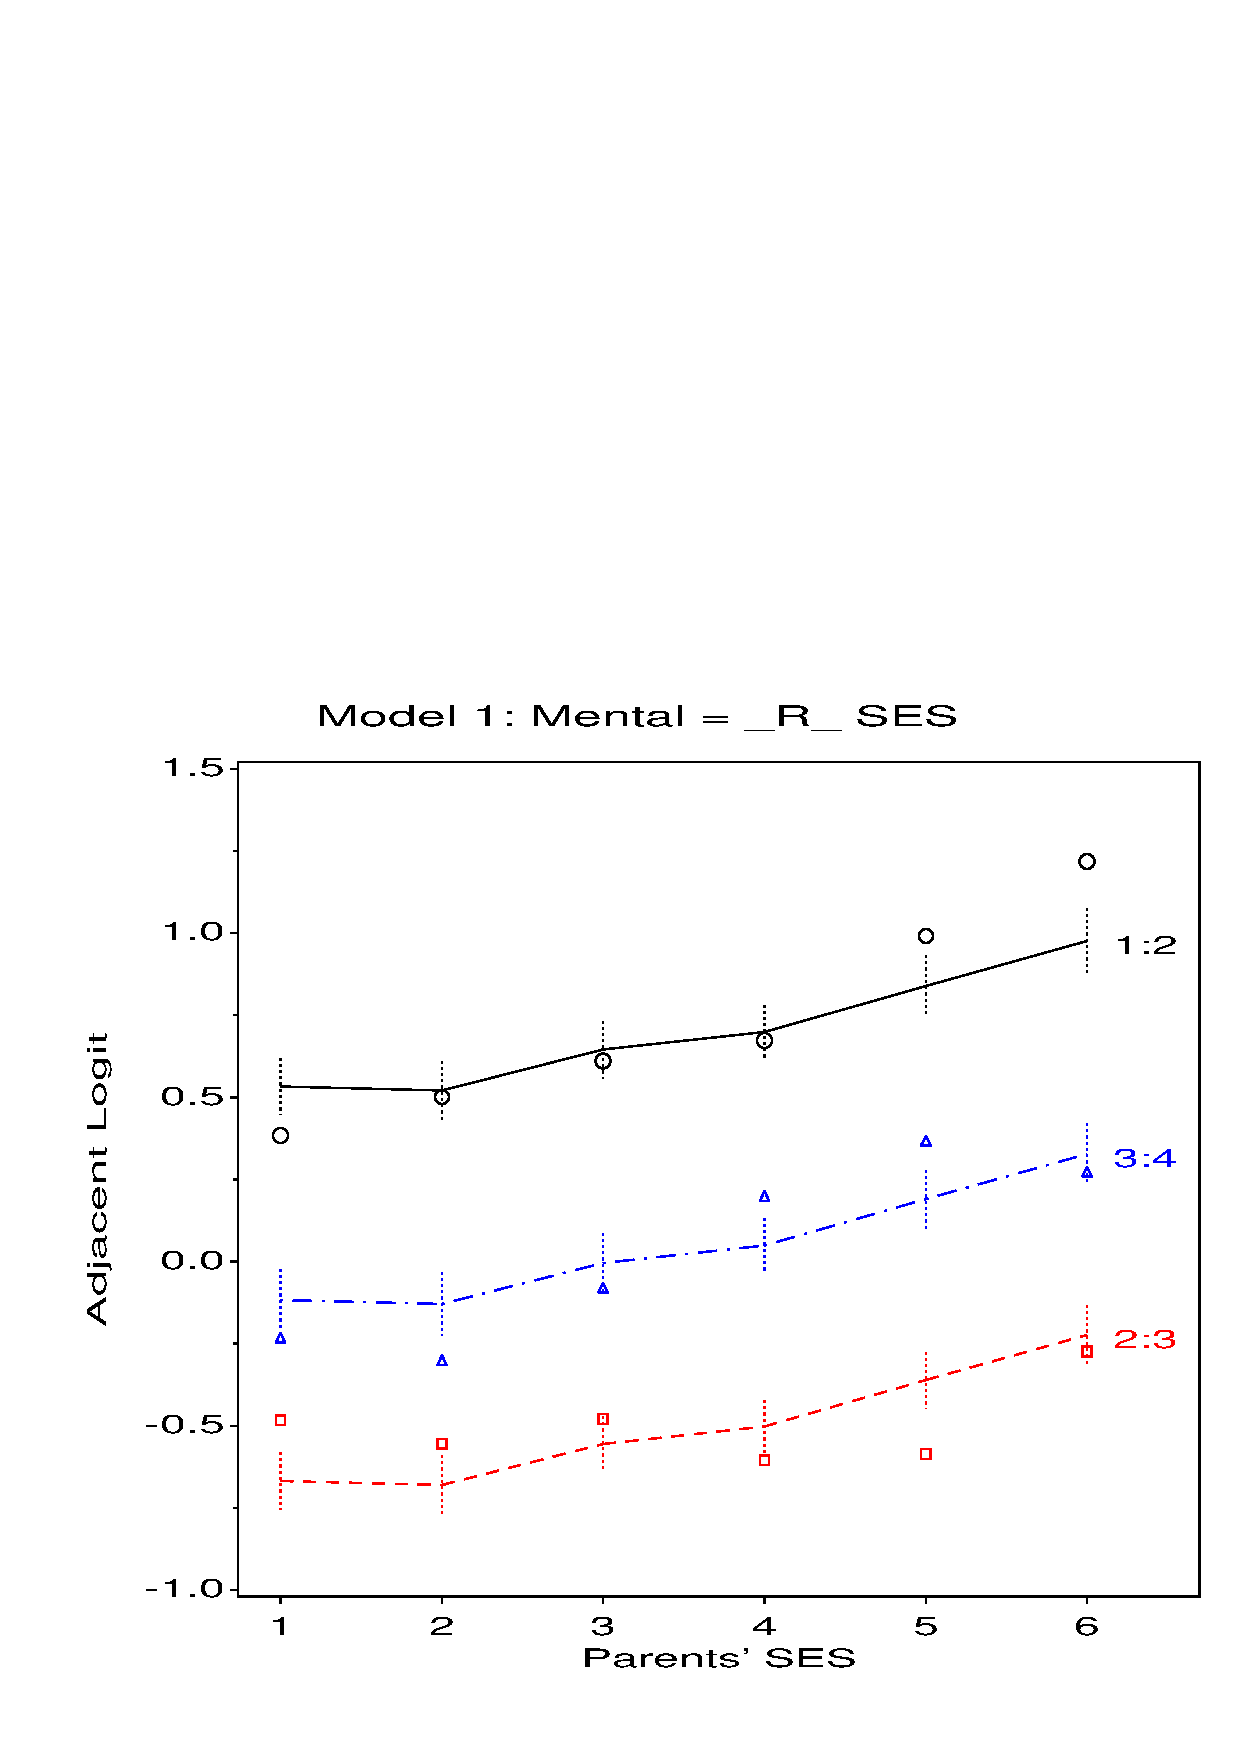
\includegraphics[width=1\linewidth]{mental41}
 \end{minipage}%
 \hfill
 \begin{minipage}[t]{.49\linewidth}
  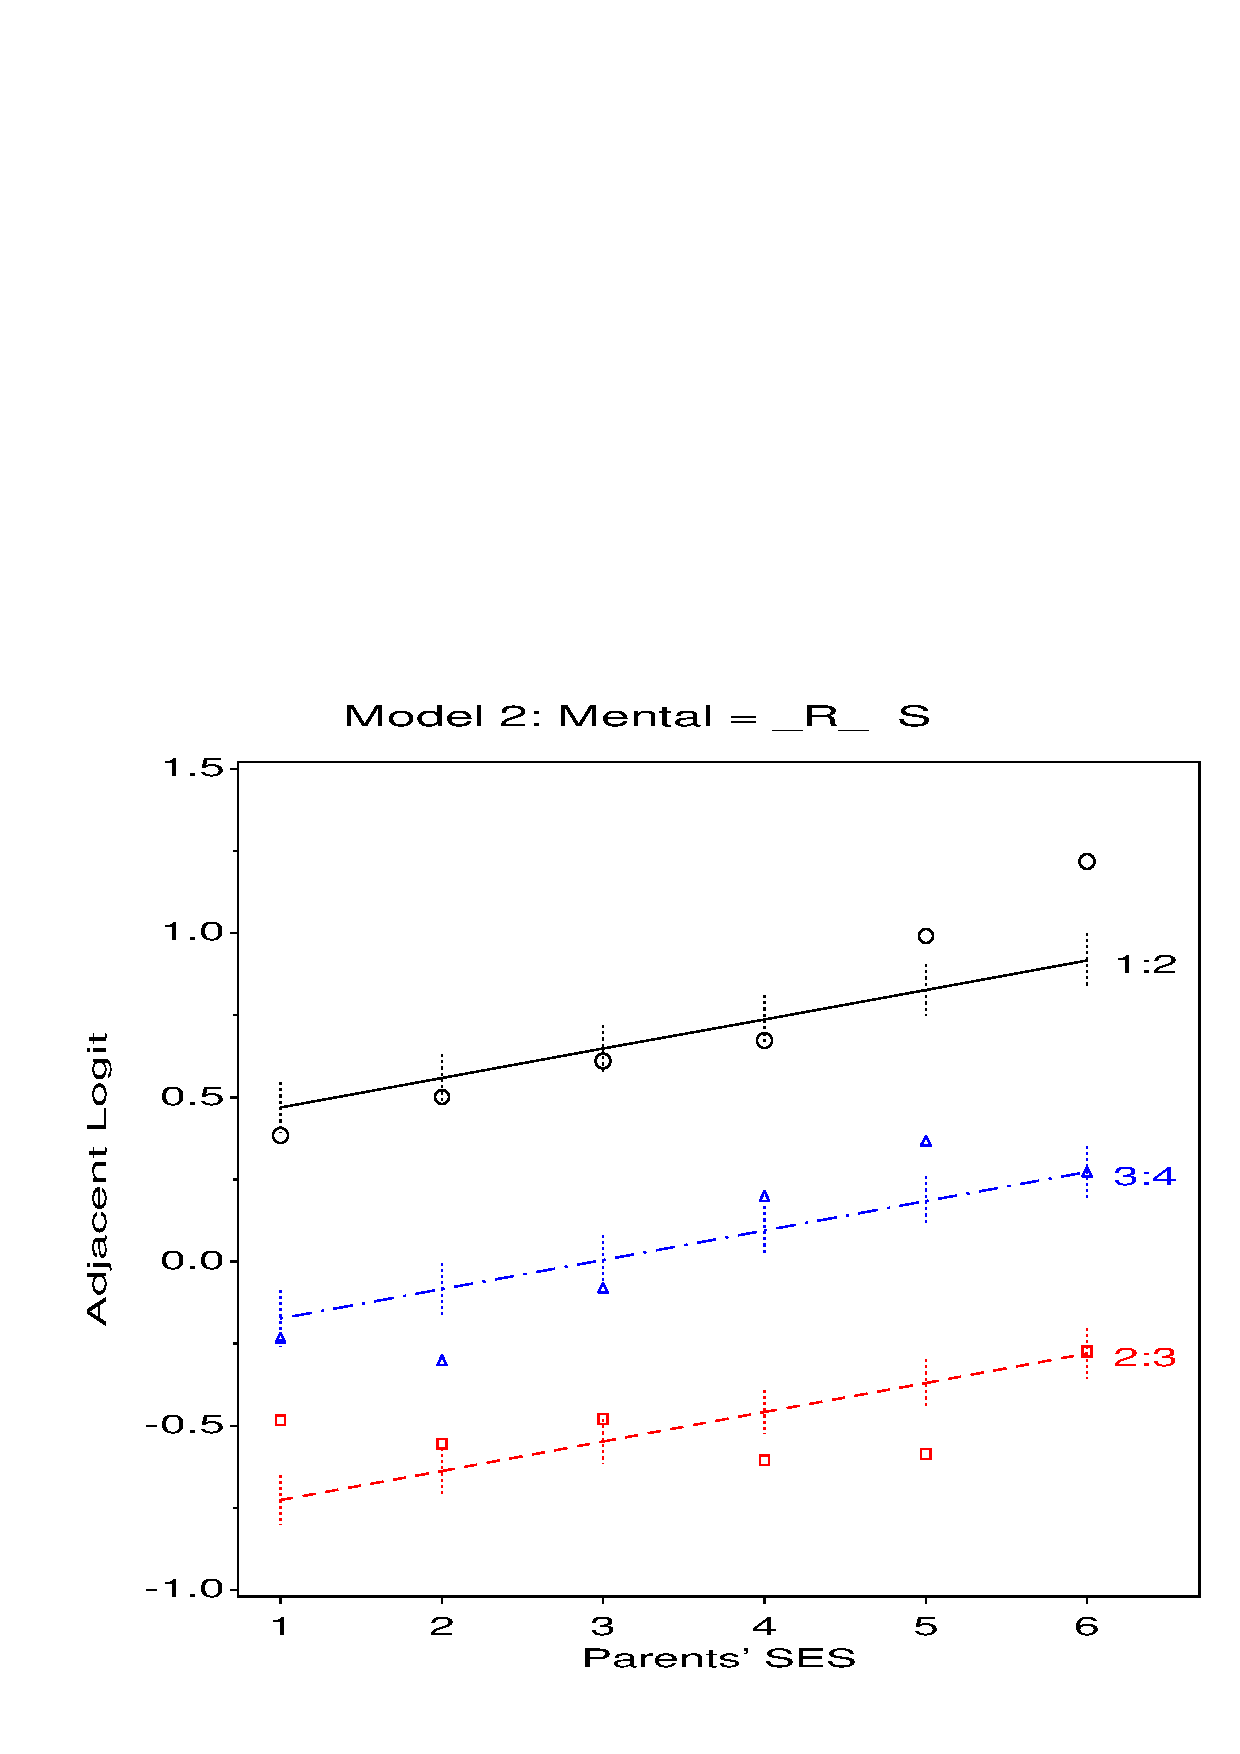
\includegraphics[width=1\linewidth]{mental42}
 \end{minipage}
 \caption{Adjacent category logit models for Mental Health data, Model 1 and Model 2}\label{fig:mental4a}
\end{figure}
\input{ch7/tab/mentab4}
For each model, an \ODS, which contains the observed and fitted logits,
is requested with the \opt{OUT=}{CATMOD} in the \stmt{RESPONSE}{CATMOD}.
Plotting the observed and fitted logits
makes it easy to see what relationships are implied by each model.
The plots for Model 1 and Model 2, shown in \figref{fig:mental4a},
are produced with the \macro{CATPLOT}
as shown below.
The macro call requests a plot of the observed logit
(\verb|_OBS_|) against \pname{SES}, with separate curves for each
adjacent logit (\verb|CLASS=_NUMBER_|).
By default, the macro also draws curves connecting the predicted
values (\verb|_PRED_| in the \ODS) and $\pm 1$ standard error bars
around each fitted logit.
\begin{listing}
axis1 label=(a=90) order=(-1 to 1.5 by .5);
axis2 offset=(3,8);
proc format;
   value cum 1='1:2'  2='2:3'  3='3:4';
title 'Model 1: Mental = _R_ SES';
%catplot(data=pred1, x=ses, y=_obs_, class=_number_, clfmt=cum.,
   type=FUNCTION, ylab=Adjacent Logit);

title 'Model 2: Mental = _R_  S';
%catplot(data=pred2, x=ses, y=_obs_, class=_number_, clfmt=cum.,
   type=FUNCTION, ylab=Adjacent Logit);
\end{listing}

For illustration, we also fit less restrictive models,
allowing a quadratic relation between the adjacent logit and SES (Model 4).
Model 5 adds a quadratic term
to the unequal slopes allowed in Model 3.
Plots for Model 3 and Model 5 are shown in \figref{fig:mental4b}.
\input{ch7/sas/mental42}

%% two subfig side-by-side
\begin{figure}[htb]
 \begin{minipage}[t]{.49\linewidth}
  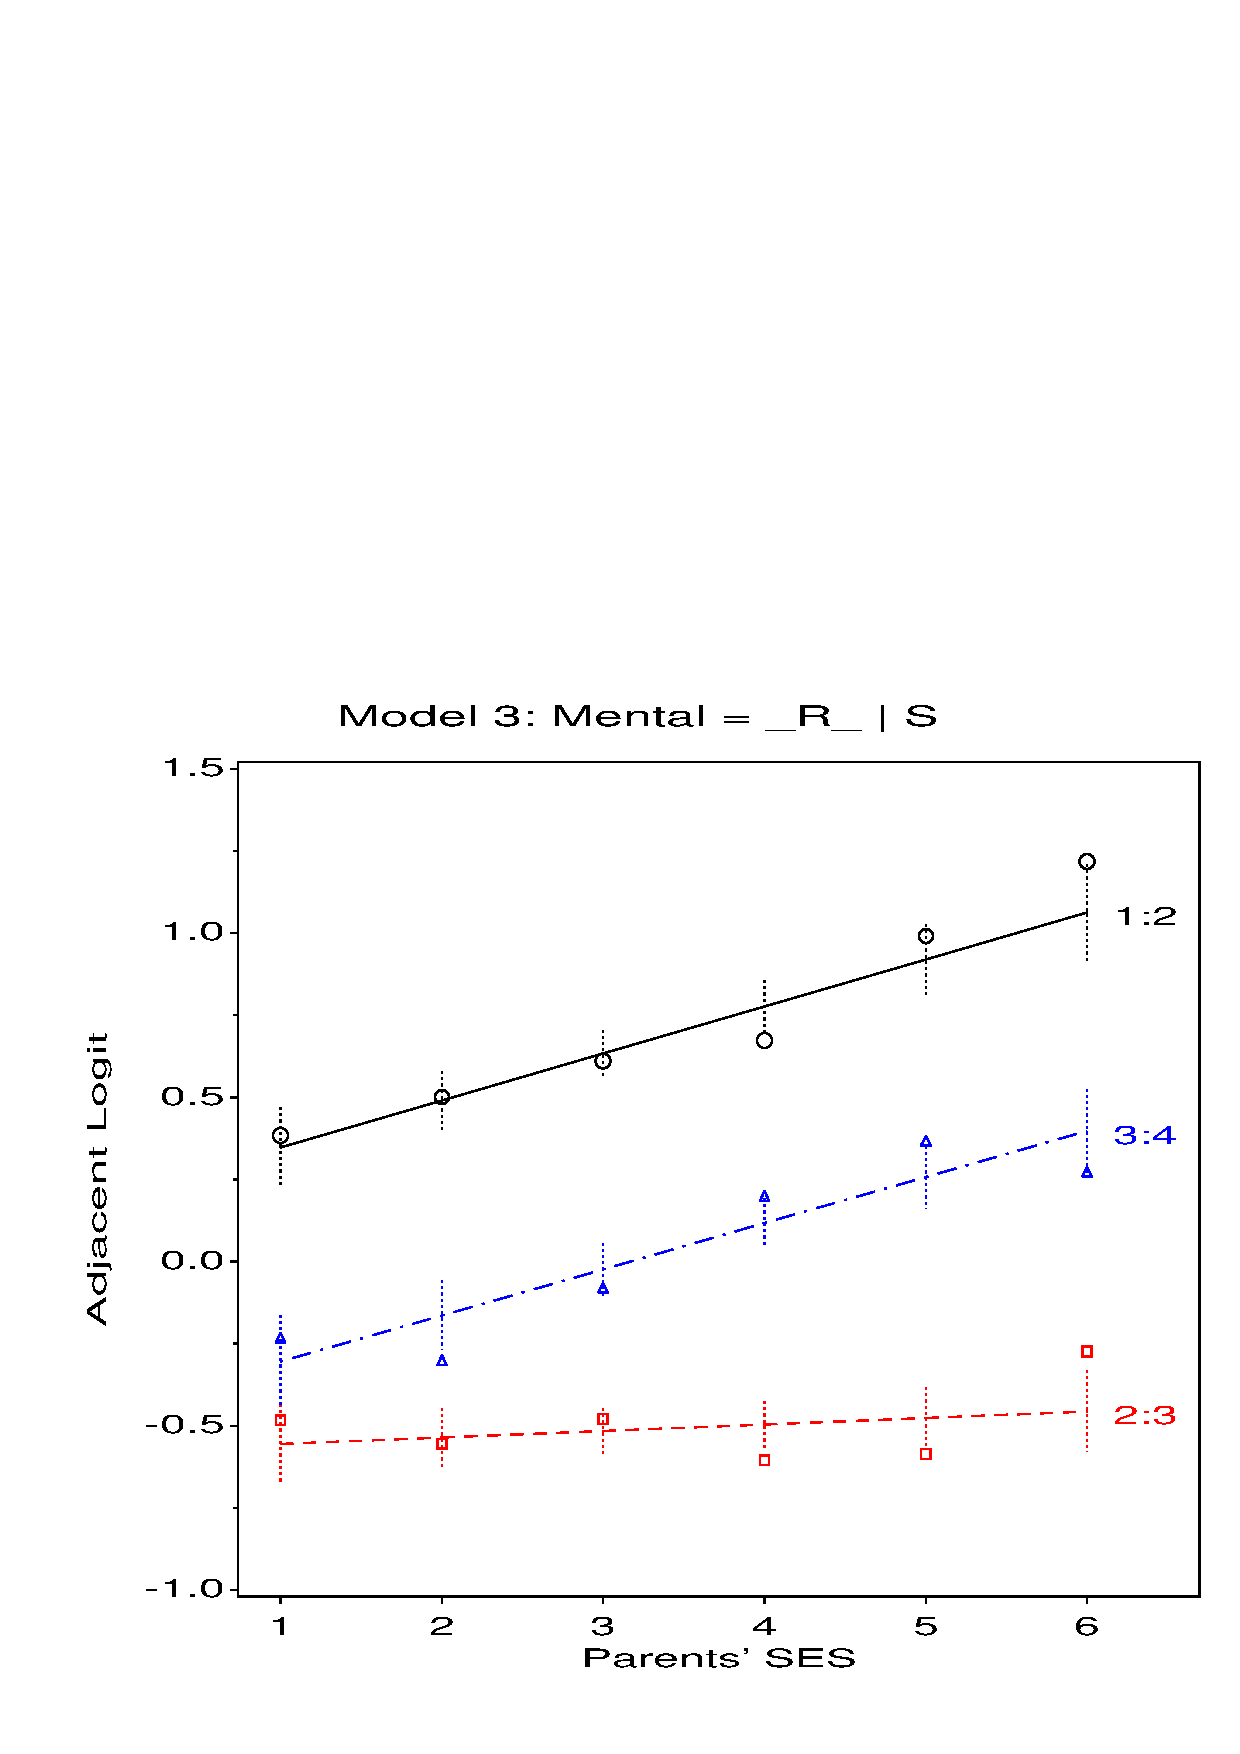
\includegraphics[width=1\linewidth]{mental43}
 \end{minipage}%
 \hfill
 \begin{minipage}[t]{.49\linewidth}
  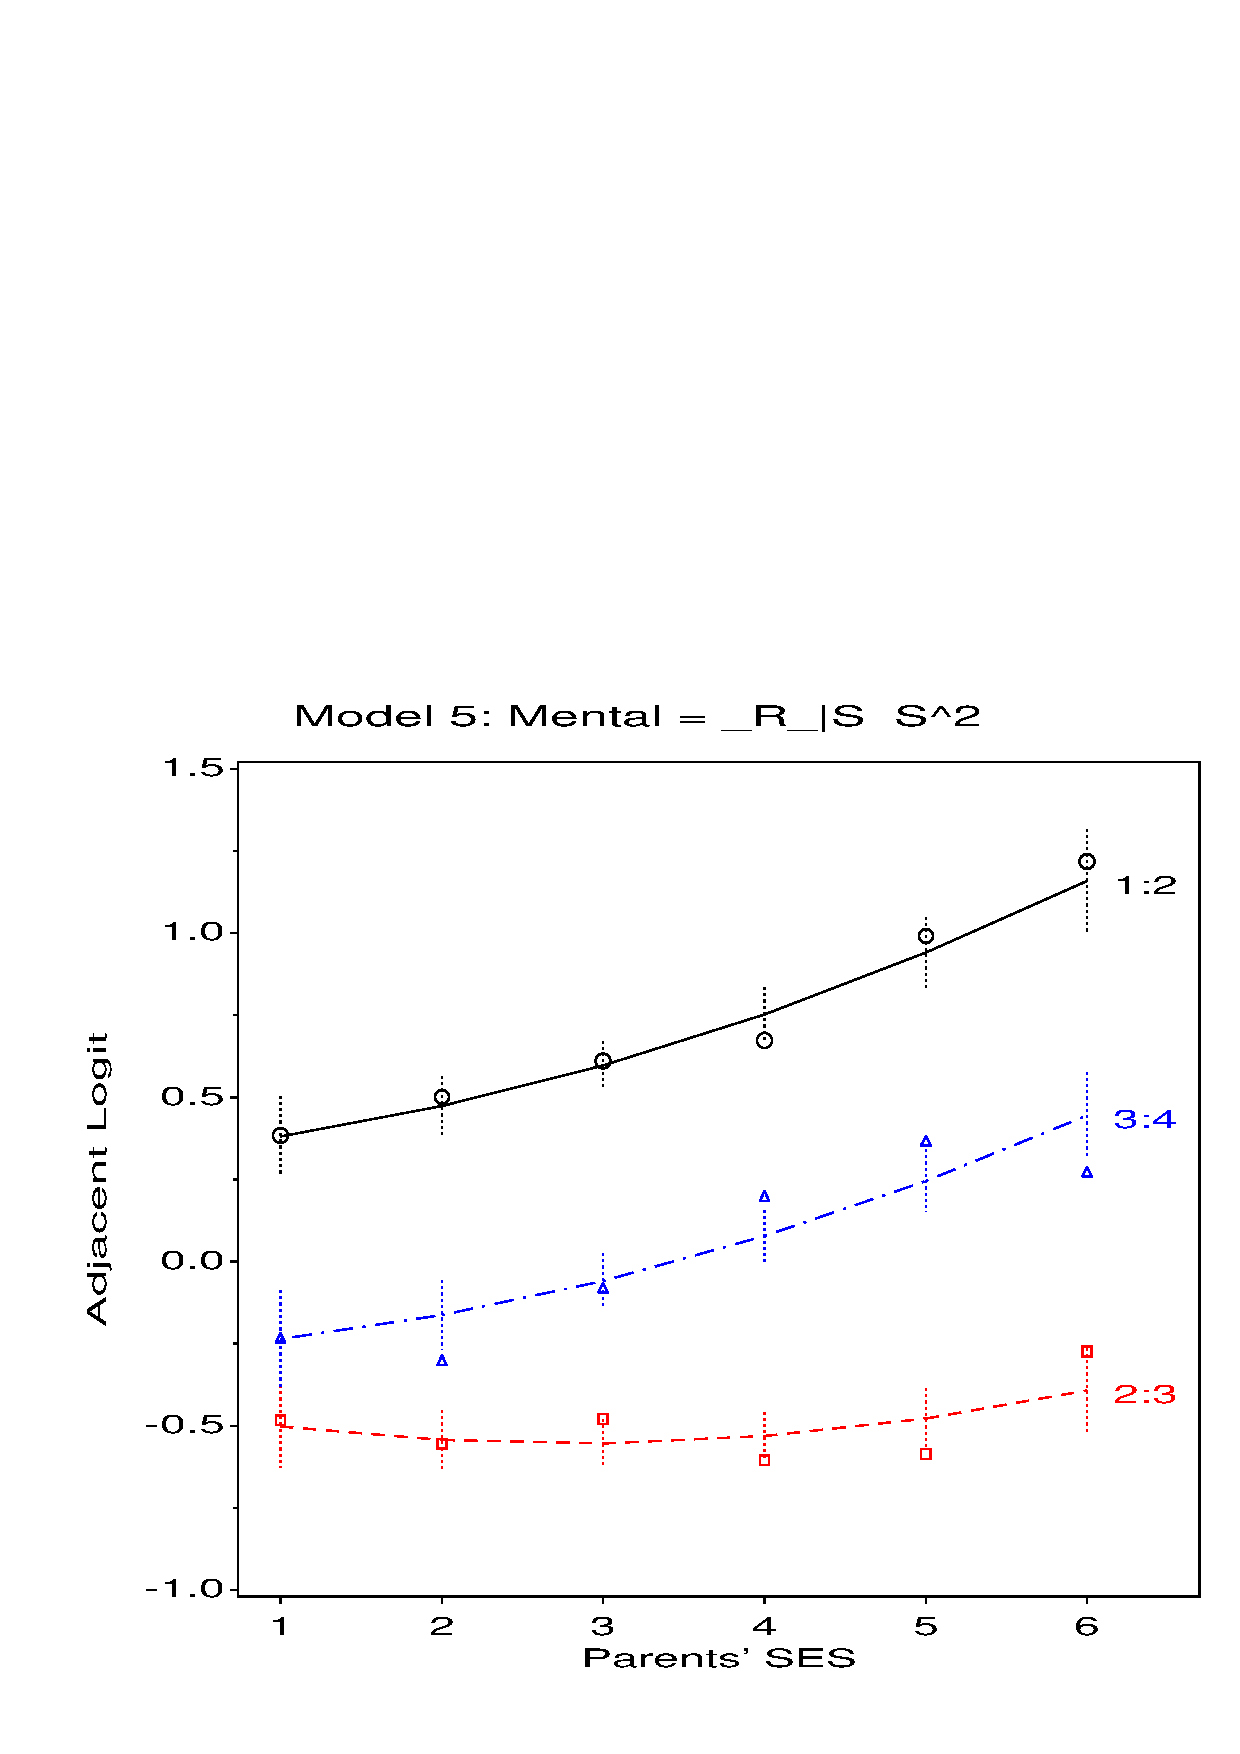
\includegraphics[width=1\linewidth]{mental44}
 \end{minipage}
 \caption{Adjacent category logit models for Mental Health data: Model 3 and Model 5}\label{fig:mental4b}
\end{figure}

What may we conclude from this?
From \tabref{tab:mentab4}, all models except the independence model
have acceptable fit according to the \chisq\ values;
Models 2--5 all have smaller AIC values than Model 1;  of these,
Model 2, the linear-by-linear is the most parsimonious, but Models
4 and 5 have slightly smaller AIC values.

One interpretation, from the plots in \figref{fig:mental4a} and \figref{fig:mental4b}
is that there is evidence that not both of SES and mental impairment
can be considered linear with unit spacing.
The intercepts suggest that the gap between categories 1 and 2
(`Well', 'Mild impairment') is greatest on the mental health scale,
and that between categories 2 and 3 (`Mild', `Moderate impairment')
is smallest.
The evidence regarding the metric for SES is more ambiguous:
there is a suggestion of a mildly quadratic relationship with SES,
particularly for the logit between response categories 1 and 2,
but this may be due to the points for (lowest) SES categories 5 and 6,
where the large logit values imply
a relatively larger number of people
classified as mildly impaired as opposed to well.
\end{Example}


\subsection{Cumulative logit models}\label{sec:loglin-ordcum}
When there is an ordinal response factor, cumulative logit models
\citep{WilliamsGrizzle:72} provide
an alternative way to take the ordinal nature of the response into account,
without assigning arbitrary scores to the response categories.

Let $F_j$ be the cumulative probability of a response less than or equal
to category $j$,
\begin{equation*}
F_j = \pi_1 + \pi_2 + \cdots + \pi_j  = \sum_{h=1}^{h=j} \pi_h
 \period
\end{equation*}
Then the \emph{cumulative logit} is defined as
\begin{equation*}%\label{eq:cumlogit}
C_j \equiv \logit ( 1 - F_j ) =
  \log \left( \frac { 1 - F_j }{F_j} \right) \period
\end{equation*}
$C_j$ gives the log odds that the response is in a category \emph{greater} than
category $j$, as opposed to a category less than or equal to $j$.
By this definition, the cumulative logits are necessarily
monotone decreasing over the response categories:
$C_1 \ge C_2 \ge \cdots \ge C_{J-1}$.
Models for the cumulative logit are particularly useful when the
response may be considered a discrete realization of an underlying
continuous variable.

In terms of cumulative logits, the model of independence is
\begin{equation*}%\label{eq:cindep}
C_{j|i} = \beta_j \comma
\end{equation*}
that is, the logit does not depend on explanatory variable(s) indexed
by subscript $i$.
Here, the response category parameters $\beta_j$ refer to the
cutpoints between adjacent categories, rather than to the distances
between adjacent ones as in the analogous adjacent category logit
model \eqref{eq:aindep}.

For quantitative scores, $a_i$, assigned to an explanatory variable,
the analog of the linear-by-linear model is
\begin{equation}\label{eq:clin}
 C_{j| i} = \beta_j + \gamma \: a_i
 \period
\end{equation}
which again has one more parameter than the independence model.
For any two rows, the difference in logits,
$C_{j| i} - C_{j| i'}$
is the log odds ratio in the $2\times 2$ table
for those two rows, with columns dichotomized following response category $j$.
Under model \eqref{eq:clin}, $C_{j| i} - C_{j| i'} = \gamma ( a_i - a_{i'})$,
so the log odds ratio is proportional to the difference in scale values,
and is the same at all cutpoints.
When unit-spaced scores, $\{a_i\} = i$ are used, the logit difference for
adjacent rows is then constant:
\begin{equation*}
 C_{j| i} - C_{j| i'} = \gamma
 \period
\end{equation*}

As with the adjacent category logits, a variety of models analogous to
the row effects model \eqref{eq:arow}, and
the linear-interaction model \eqref{eq:alin-int}
may be defined for the cumulative logits.
We illustrate these below, primarily to look at the shapes of plots
of observed and fitted logits, and to compare them with what we saw for
adjacent category logits.
\begin{Example}[mental3]{Mental impairment and parents' SES}
Cumulative logit models may be fit using \PROC{CATMOD} with the
\pname{RESPONSE CLOGIT;} statement.
The model is specified in the same way as for adjacent category
logits, but now the \verb|_RESPONSE_| keyword refers to
differences among the cumulative response probabilities.
As before,
an independent variable is treated as a quantitative variable,
when it is declared in a \stmt{DIRECT}{CATMOD}.

The following statements fit
the same models as in \exref{ex:mental4}: first Models 0--3
in which SES has no effect on mental health (Model 0), then SES with
a nominal effect (Model 1), a constant linear effect (Model 2)
and different linear effects for each cumulative logit (Model 3).
\input{ch7/sas/mental31}

For comparison, we also fit models with both linear and quadratic
effects on the cumulative logits,
first with equal slopes and curvature
for all response categories (Model 4), and second with separate slopes and
equal curvatures (Model 5).
\input{ch7/sas/mental32}

The model fit statistics for these models are shown in \tabref{tab:mentab3}.
The values are quite similar to those for the adjacent category logits
(\tabref{tab:mentab2}).
\input{ch7/tab/mentab3}

For any such model, the \macro{CATPLOT} displays the observed and fitted
cumulative logits using the \ODS\ specified on the
\stmt{RESPONSE}{CATMOD}.
The statements below produce the graphs of the logits for Model 0,
and Model 1,
shown in \figref{fig:mental3a}.
Similar statements, using the \ODS s \pname{PRED2} and \pname{PRED4},
give the graphs for Model 2 and Model 4 in \figref{fig:mental3b}.
\input{ch7/sas/mental33}

%% two subfig side-by-side
\begin{figure}[htb]
 \begin{minipage}[t]{.49\linewidth}
  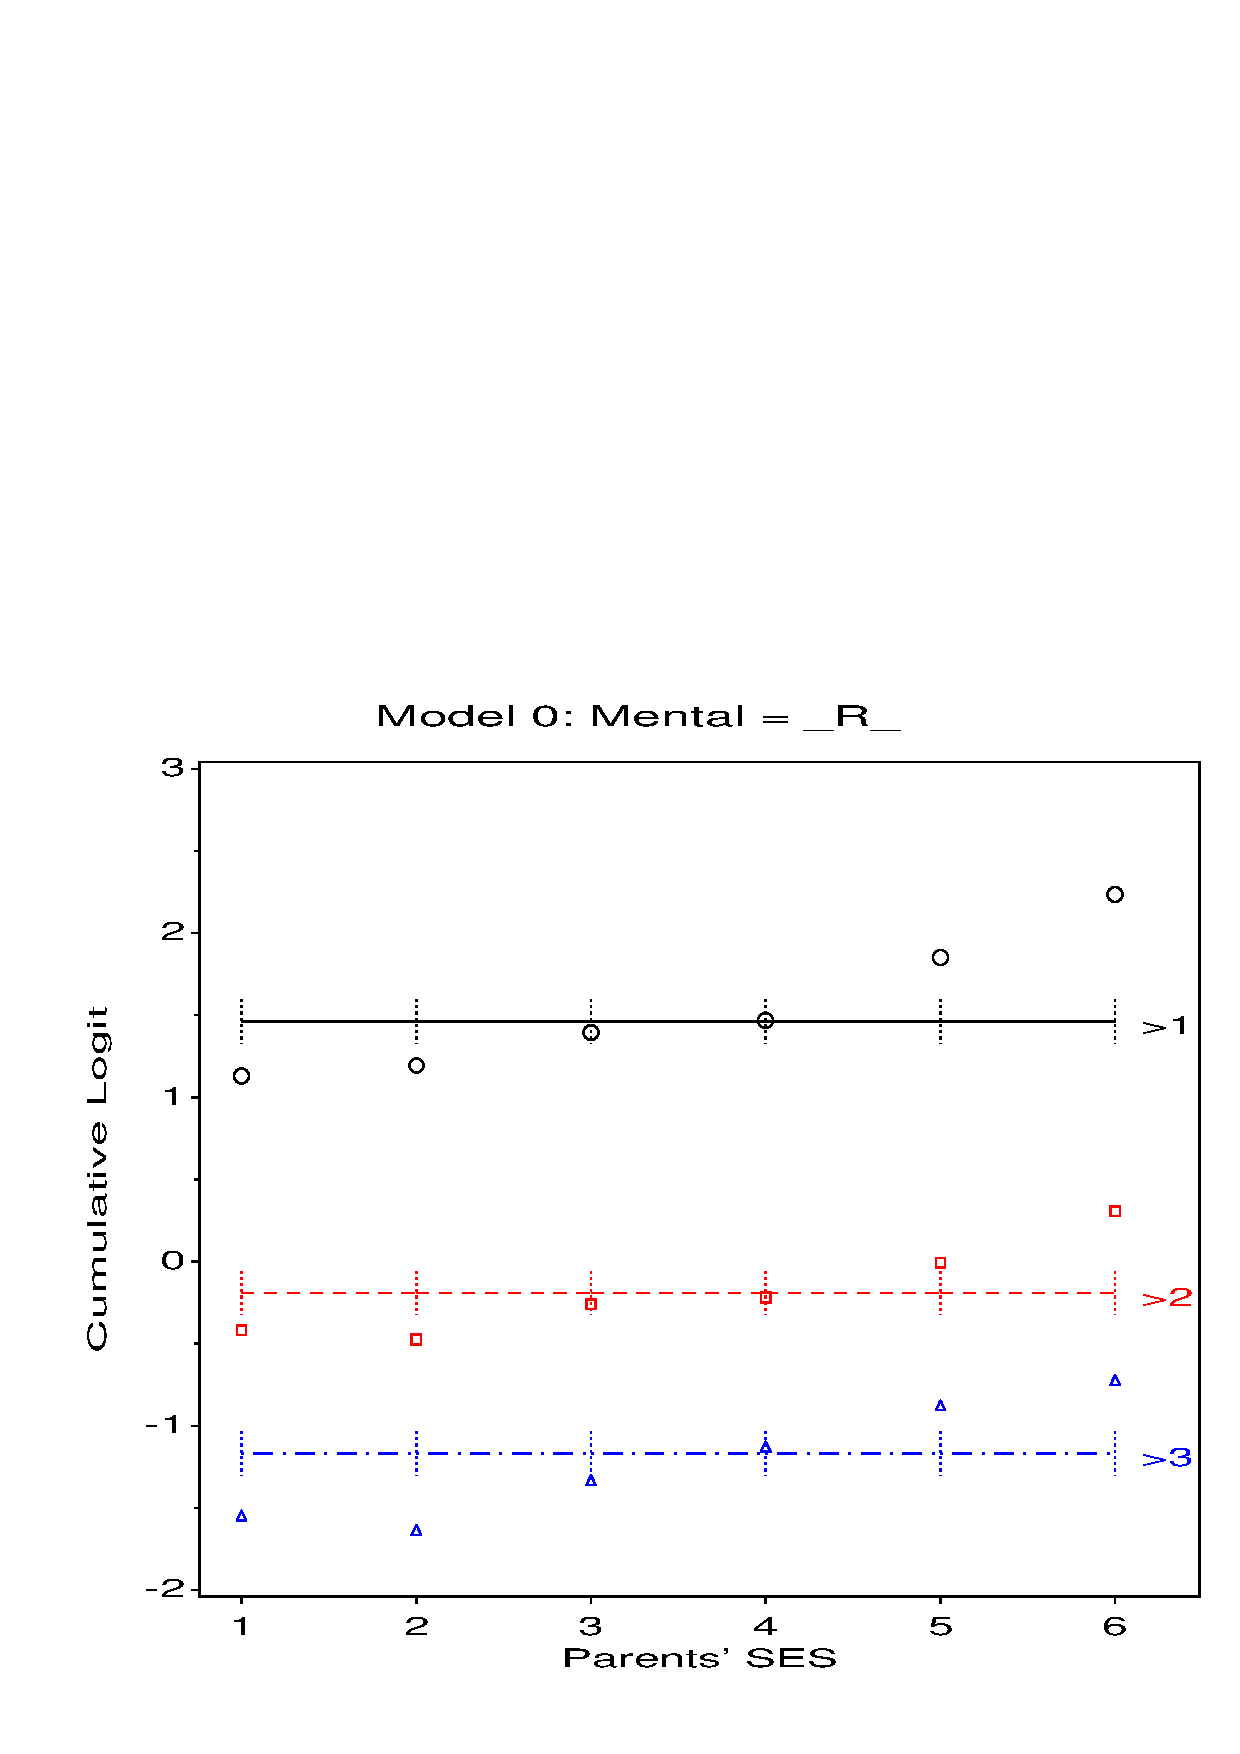
\includegraphics[width=1\linewidth]{mental31}
 \end{minipage}%
 \hfill
 \begin{minipage}[t]{.49\linewidth}
  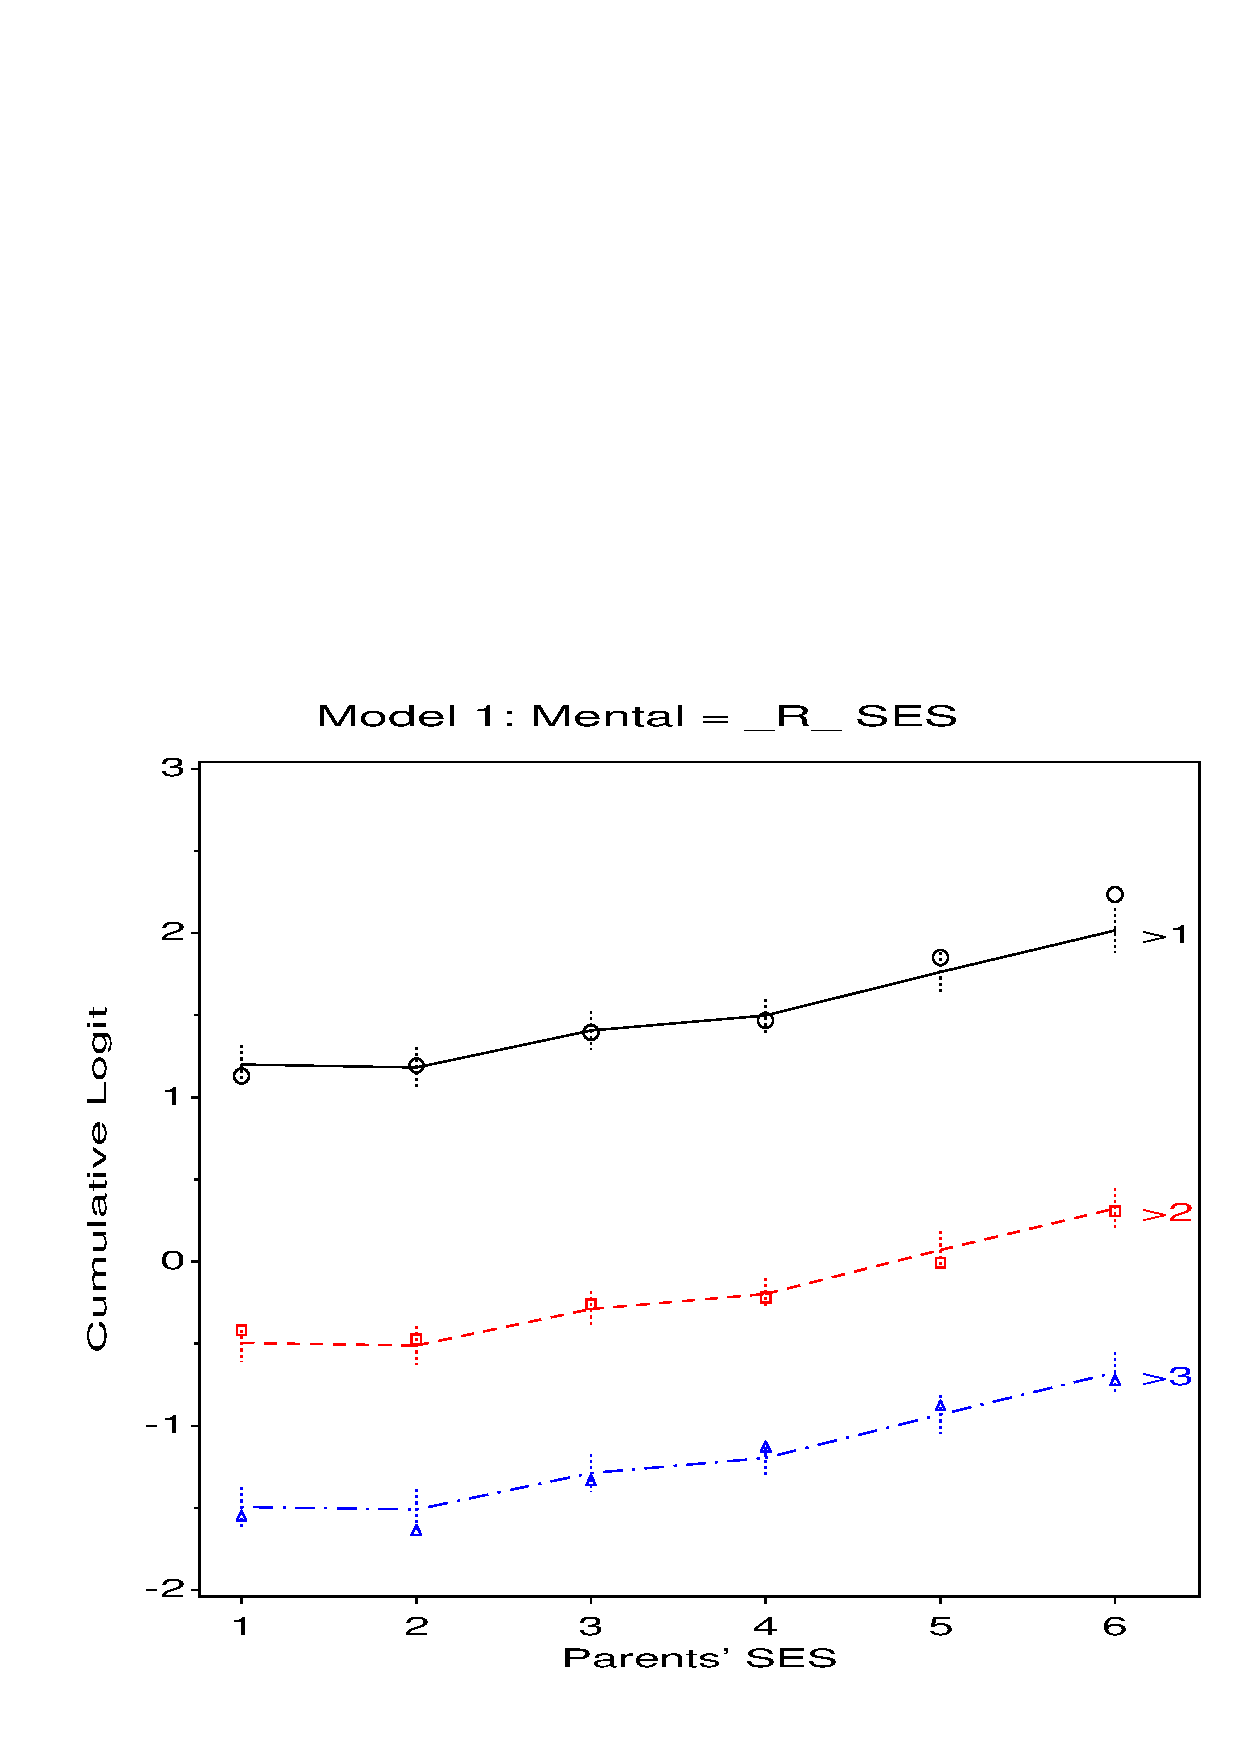
\includegraphics[width=1\linewidth]{mental32}
 \end{minipage}
 \caption{Cumulative logit models for Mental Health data, Model 0 and Model 1}\label{fig:mental3a}
\end{figure}

%% two subfig side-by-side
\begin{figure}[htb]
 \begin{minipage}[t]{.49\linewidth}
  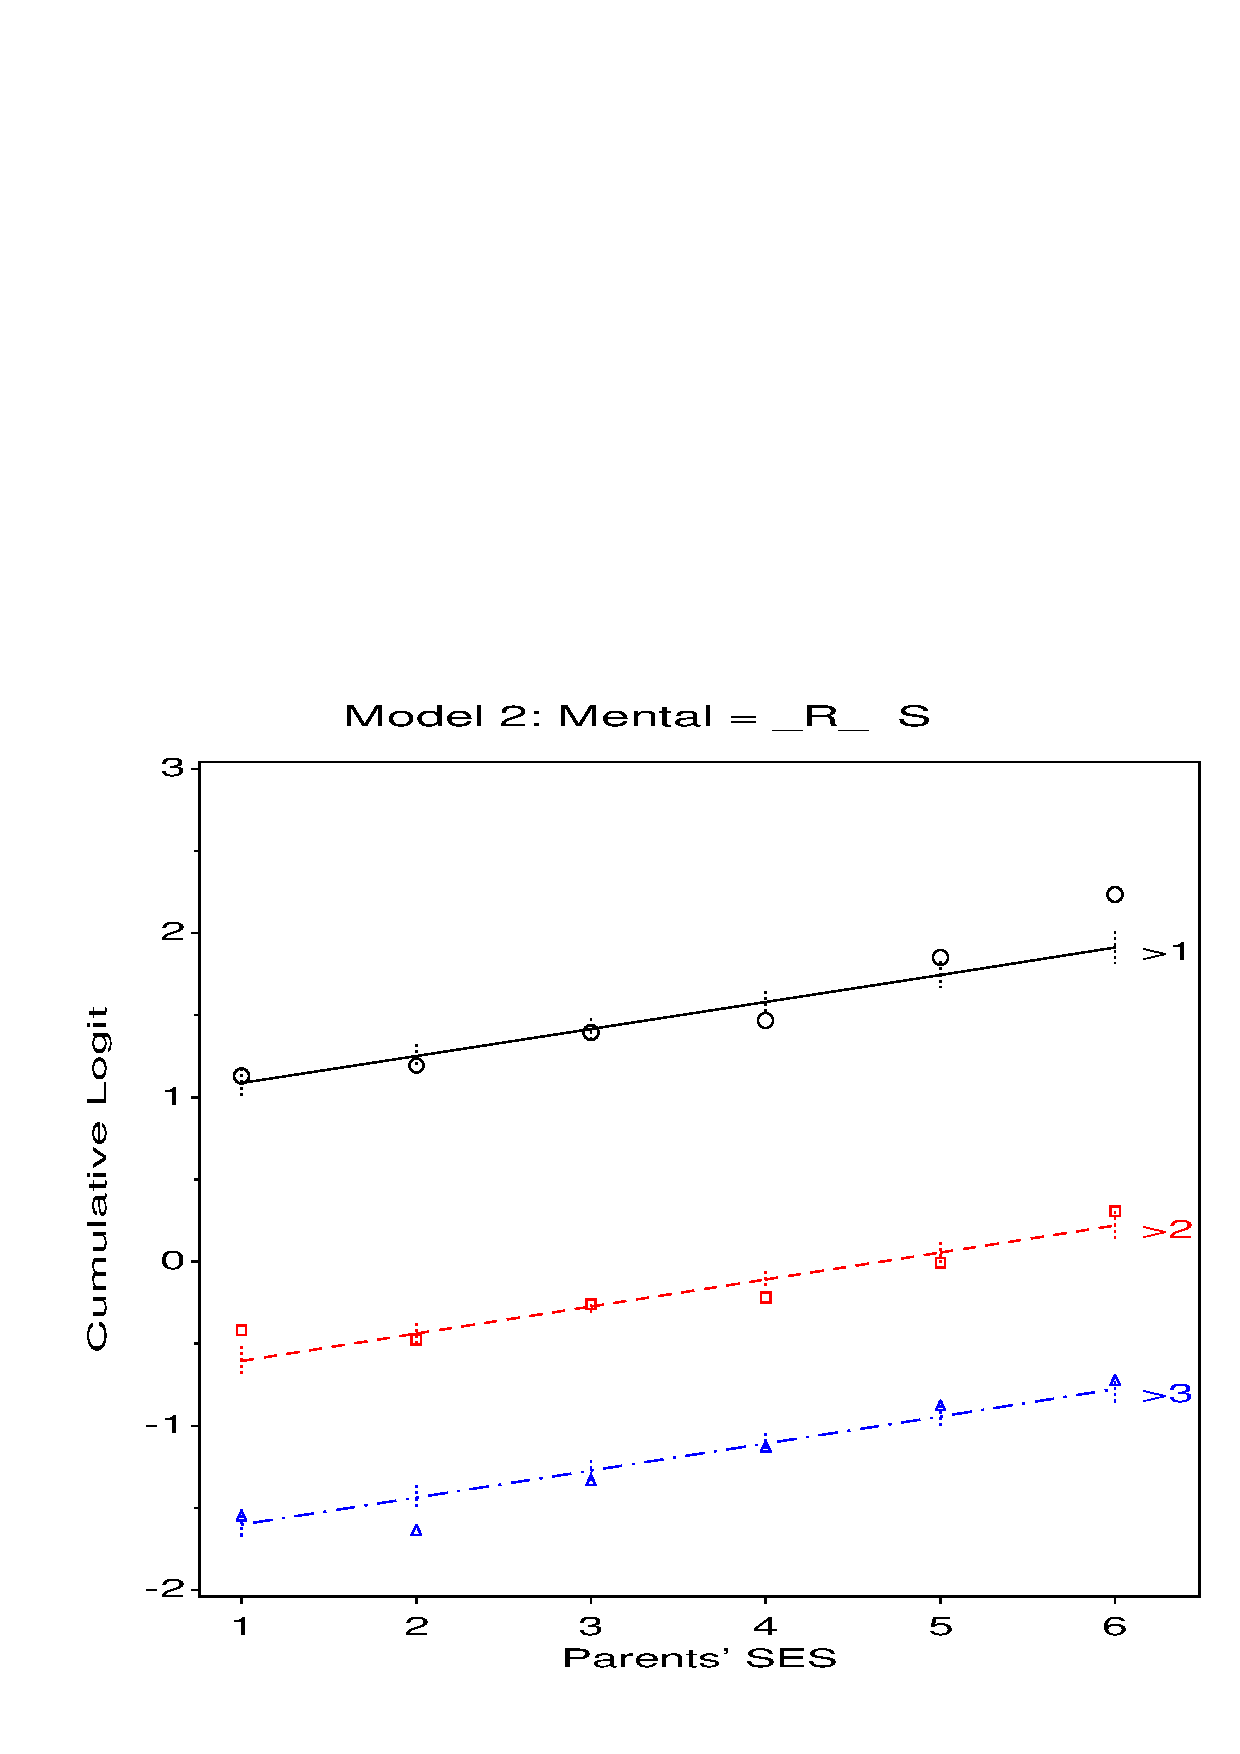
\includegraphics[width=1\linewidth]{mental33}
 \end{minipage}%
 \hfill
 \begin{minipage}[t]{.49\linewidth}
  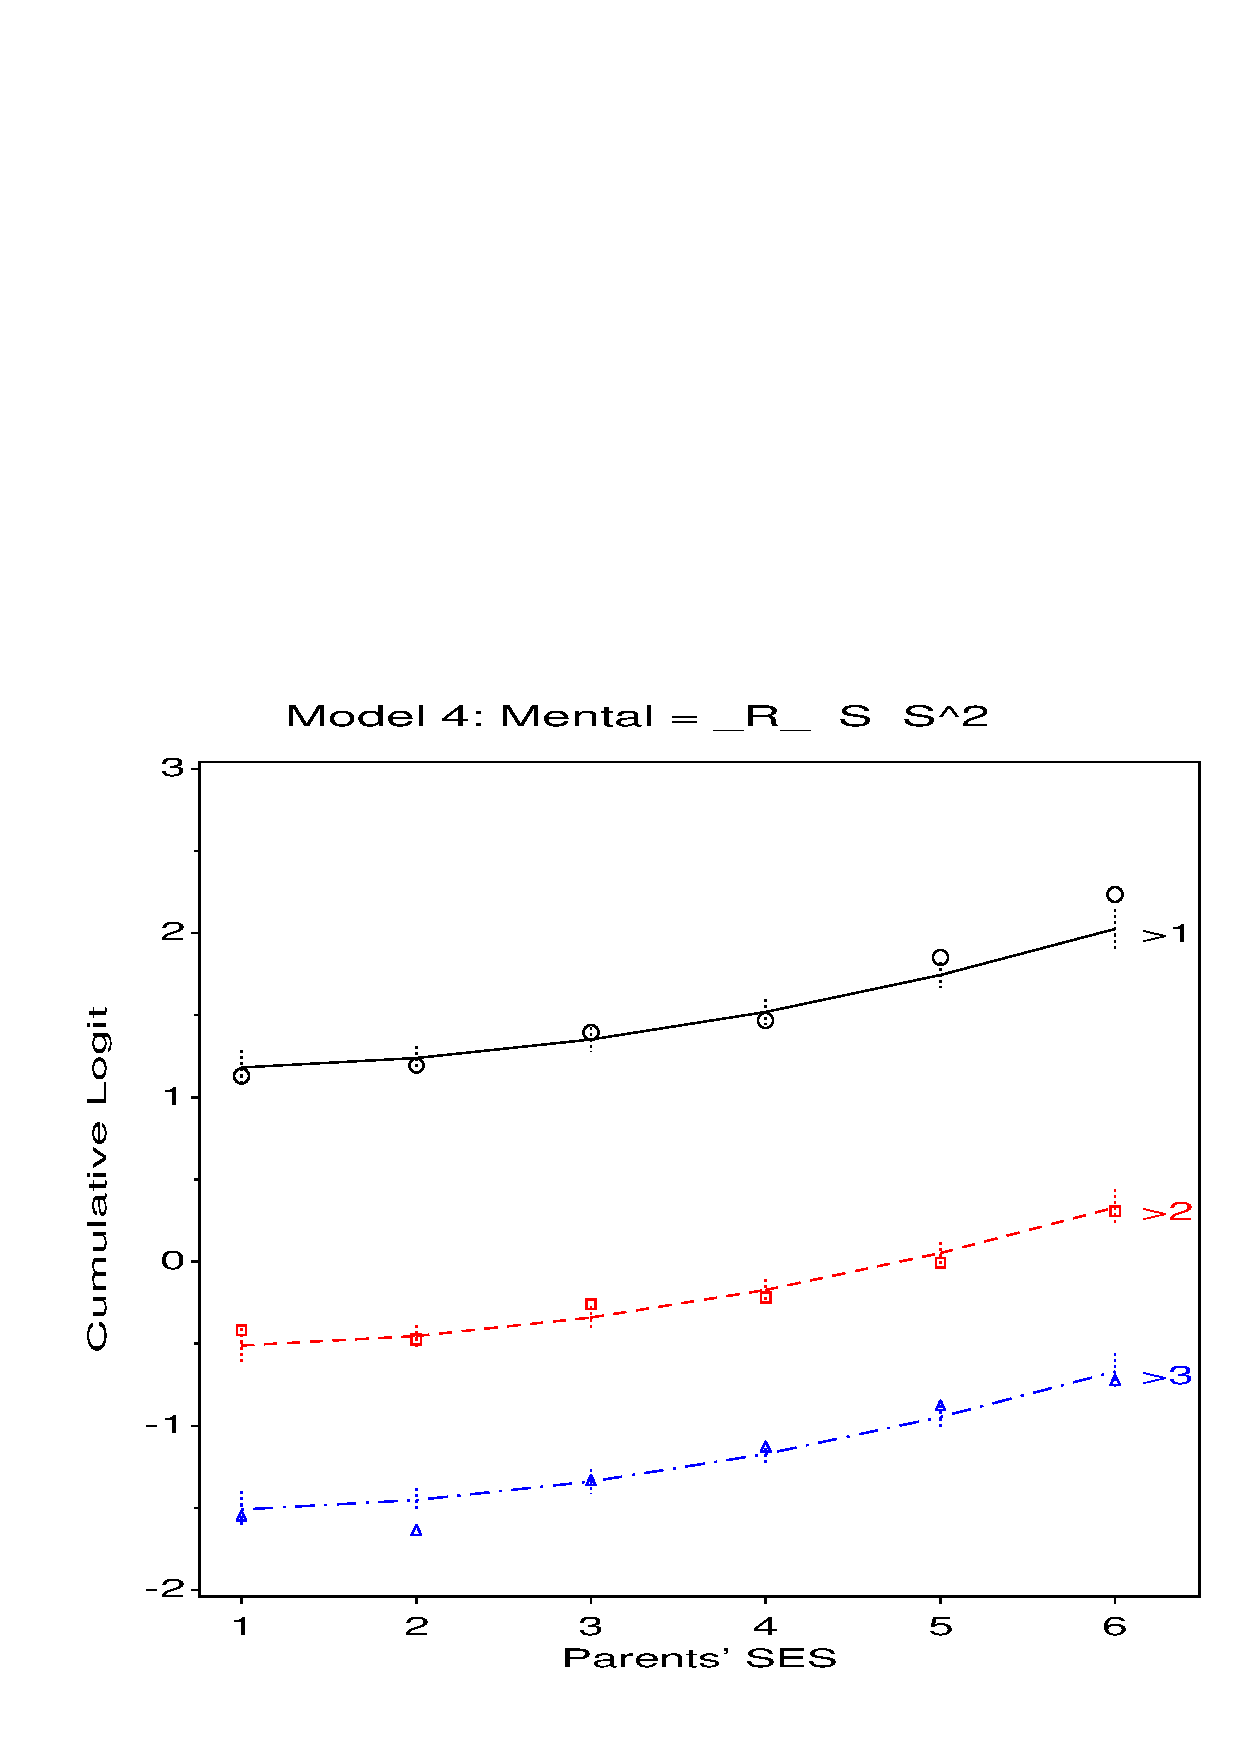
\includegraphics[width=1\linewidth]{mental35}
 \end{minipage}
 \caption{Cumulative logit models for Mental Health data: Model 2 and Model 4}\label{fig:mental3b}
\end{figure}
\end{Example}

\subsection{Nested dichotomies}\label{sec:nested}

Nested dichotomies are successive binary partitions of the response
categories into nested sets.  For the levels of
a factor in an ANOVA design, nested dichotomies correspond to
orthogonal contrasts (assuming equal $n$s).

For example, the response categories
\{1,2,3,4\} could be divided first as \{1,2\} vs. \{3,4\}, as shown in the
left side of \figref{fig:nested}.  Then these two
dichotomies could be divided as \{1\} vs. \{2\}, and \{3\} vs. \{4\}.
Alternatively, these response categories could be divided as shown in the
right side of \figref{fig:nested}: first, \{1\} vs.
\{2,3,4\}, then \{2\} vs \{3,4\}, and finally \{3\} vs. \{4\}.  
\begin{figure}[htb]
  \centering
  \includegraphics[scale=.5]{ch6/fig/nested}
  \caption[Nested dichotomies]{Nested dichotomies.  The boxes show two different ways a four-category response can be represented as three nested dichotomies. Adapted from \citet{Fox:97}.}\label{fig:nested}
\end{figure}

Then,
\begin{itemize}

\item Each dichotomy can be fit using the familiar binary-response
 logistic model, and,
\item When the dichotomies are nested, the \(m - 1\) models will be statistically independent, so
that likelihood-ratio \(G^2\) statistics for overall fit, and
Wald statistics for individual terms will be additive.
\end{itemize}
Thus, we can treat the set of \(m - 1\) models as a single model
for the polytomous response, although we fit them separately for
computational purposes.  This approach to polytomous responses
is described in more detail by \citet{Fox:97}.

\begin{Example}[wlfpart]{Women's labor-force participation}
To illustrate, \citet{Fox:84,Fox:97} presented survey data on women's labor-force
participation in Canada in 1977.  Women were classified as not working
outside the home (n=155), working part-time (n=42)  or working
full-time (n=66).  Predictor variables were presence/absence of
children, and husband's income; a third variable, region of Canada,
is not considered here.  For these data, it makes sense to model the
log odds for two nested dichotomies:

\begin{itemize*}
\item Working vs. NotWorking
\item Working fulltime vs working parttime.
\end{itemize*}

The data are read in as shown below.
See \datref{dat:wlfdata} for the complete \Dset.  The 3-level variable
\pname{labor} is used to define two dichotomous variables, \pname{working}, and \pname{fulltime}.  Note that \pname{fulltime} is defined
(has non-missing values) only for working women.

\begin{listing}
proc format;
   value labor    /* labor-force participation */
      1 ='working full-time'  2 ='working part-time'
      3 ='not working';
   value kids     /* presence of children in the household */
      0 ='Children absent'  1 ='Children present';
data wlfpart;
   input case labor husinc children region;
   working = labor < 3;
   if working then
      fulltime = (labor = 1);
datalines;
  1  3  15  1  3
  2  3  13  1  3
  3  3  45  1  3
  4  3  23  1  3
  5  3  19  1  3
  {\it ... more data lines ...}
\end{listing}

An initial analysis attempts to fit the proportional odds model, with
the 3-level \pname{labor} variable as the response:

\begin{listing}
proc logistic data=wlfpart nosimple;
   {\bf model labor  = husinc children ;}
   title2 'Proportional Odds Model for Fulltime/Parttime/NotWorking';
\end{listing}

However, the proportional odds assumption is rejected by the score
test (see \outref{out:wlfpart.1}).

\begin{Output}[htb]
\caption{Test of the proportional odds assumption}\label{out:wlfpart.1}
\small
\begin{output}
          Score Test for the Proportional Odds Assumption

             Chi-Square = 18.5641 with 2 DF (p=0.0001)
\end{output}
\end{Output}

Hence, we fit models for each of the \pname{working} and \pname{fulltime}
dichotomies.  The \opt{descending}{LOGISTIC} is used so that in each
case the probability of a 1 response (working, or fulltime) will be
the event modeled.

\begin{listing}
proc logistic data=wlfpart nosimple descending;
   {\bf model working = husinc children ;}
   output out=resultw p=predict xbeta=logit;
   title2 'Nested Dichotomies';
run;
proc logistic data=wlfpart nosimple descending;
   {\bf model fulltime = husinc children ;}
   output out=resultf p=predict xbeta=logit;
\end{listing}

The \stmt{output}{LOGISTIC}s  create the \Dsets\ \pname{resultw} and
\pname{resultf} for plotting the predicted probabilities and logits.
The printed output for the working dichotomy is shown (partially)
in \outref{out:wlfpart.2}.

\begin{Output}[htb]
\caption{Women's labor-force data, analysis of the working/not working dichotomy}\label{out:wlfpart.2}
\small
\begin{output}
                               Response Profile
                          Ordered
                            Value  WORKING     Count

                                1        1       108
                                2        0       155

                  Testing Global Null Hypothesis: BETA=0
                            Intercept
               Intercept       and
   Criterion     Only      Covariates    Chi-Square for Covariates

   AIC           358.151      325.733      .
   SC            361.723      336.449      .
   -2 LOG L      356.151      319.733    36.418 with 2 DF (p=0.0001)
   Score            .            .       35.713 with 2 DF (p=0.0001)

                    Analysis of Maximum Likelihood Estimates

               Parameter Standard    Wald       Pr >    Standardized    Odds
   Variable DF  Estimate   Error  Chi-Square Chi-Square   Estimate     Ratio

   INTERCPT 1     1.3358   0.3838    12.1165     0.0005            .    .
   HUSINC   1    -0.0423   0.0198     4.5751     0.0324    -0.168541   0.959
   CHILDREN 1    -1.5756   0.2923    29.0651     0.0001    -0.398992   0.207
\end{output}
\end{Output}

To interpret the parameter estimates, note that the odds ratio of 0.959
for husband's income
means a 4\% decrease in the odds of working with each \$1000 increase in husband's income; an additional \$10,000 means a decrease in the odds
of working by
\(e^{-.423} = .655\).  Similarly, the effect of having children  corresponds
to an odds of working of .207 compared to those without children.

The output for the fulltime vs. parttime dichotomy is shown in
\outref{out:wlfpart.3}.
Note that nonworking women are excluded in this analysis.

\begin{Output}[htb]
\caption{Women's labor-force data, analysis of the fulltime/parttime dichotomy}\label{out:wlfpart.3}
\small
\begin{output}
                                Response Profile
                          Ordered
                            Value  FULLTIME     Count

                                1         1        66
                                2         0        42

   WARNING: 155 observation(s) were deleted due to missing values for
           the response or explanatory variables.

                   Testing Global Null Hypothesis: BETA=0
                             Intercept
                Intercept       and
   Criterion      Only      Covariates   Chi-Square for Covariates

   AIC            146.342      110.495      .
   SC             149.024      118.541      .
   -2 LOG L       144.342      104.495    39.847 with 2 DF (p=0.0001)
   Score             .            .       35.150 with 2 DF (p=0.0001)

                    Analysis of Maximum Likelihood Estimates

               Parameter Standard    Wald       Pr >    Standardized    Odds
   Variable DF  Estimate   Error  Chi-Square Chi-Square   Estimate     Ratio

   INTERCPT 1     3.4778   0.7671    20.5537     0.0001            .    .
   HUSINC   1    -0.1073   0.0392     7.5063     0.0061    -0.424867   0.898
   CHILDREN 1    -2.6515   0.5411    24.0135     0.0001    -0.734194   0.071
\end{output}
\end{Output}

Thus, the full 3-category response has been fitted by two models,

\begin{eqnarray}
  \log \left( \frac{ \Pr ( \mbox{working} ) }
  { \Pr ( \mbox{not working} ) } \right) & = &
  1.336 - 0.042 \,  \mbox{H\$} - 1.576 \,  \mbox{kids} \label{eq:wlfnest1}\\
%
  \log \left( \frac{ \Pr ( \mbox{fulltime} ) }
  { \Pr ( \mbox{parttime} ) } \right) & = &
  3.478 - 0.107 \,  \mbox{H\$} - 2.652 \,  \mbox{kids} \label{eq:wlfnest2}
\end{eqnarray}
The second equation gives the predicted log odds for
fulltime vs.\ parttime work {\it conditional} on working.

Because these models are nested, we can add the likelihood ratio or Wald tests across the
\ix{likelihood ratio test}
\ix{Wald test}
two models, so the overall test of the hypothesis that neither
husband's income nor presence of children predicts working status
(the 3-level response) has a \(G^2 = 36.42  +  39.85 = 66.27\) on
2+2=4 df (\(p < .0001\)).  Similarly, the hypothesis that husband's
income does not predict working status has a Wald-test \(G^2 = 4.58
+  7.51 = 12.09\) on 2 df (\(p < .001\)).

Comparison of the regression coefficients in the two sub-models (in
relation to the size of their standard errors) indicates why the
proportional odds model was not tenable.  The proportional odds model
requires that the coefficients for husband's income and children in
analogous models of the form \eqref{eq:logod1} and \eqref{eq:logod2}.
We can see that both variables have a
greater effect on the odds of fulltime vs. parttime work than on the
odds of working vs. not working.

As usual, these effects can be seen and interpreted more easily in a
graph (\figref{fig:wlfpart}).  The odds of working outside the home decrease as husband's
income increases and when there are children present.  However, among
working women, the odds of fulltime vs. parttime work decrease at a
faster rate with husband's income; women with children are less
likely to work fulltime.
\begin{figure}[htb]
  \centering
  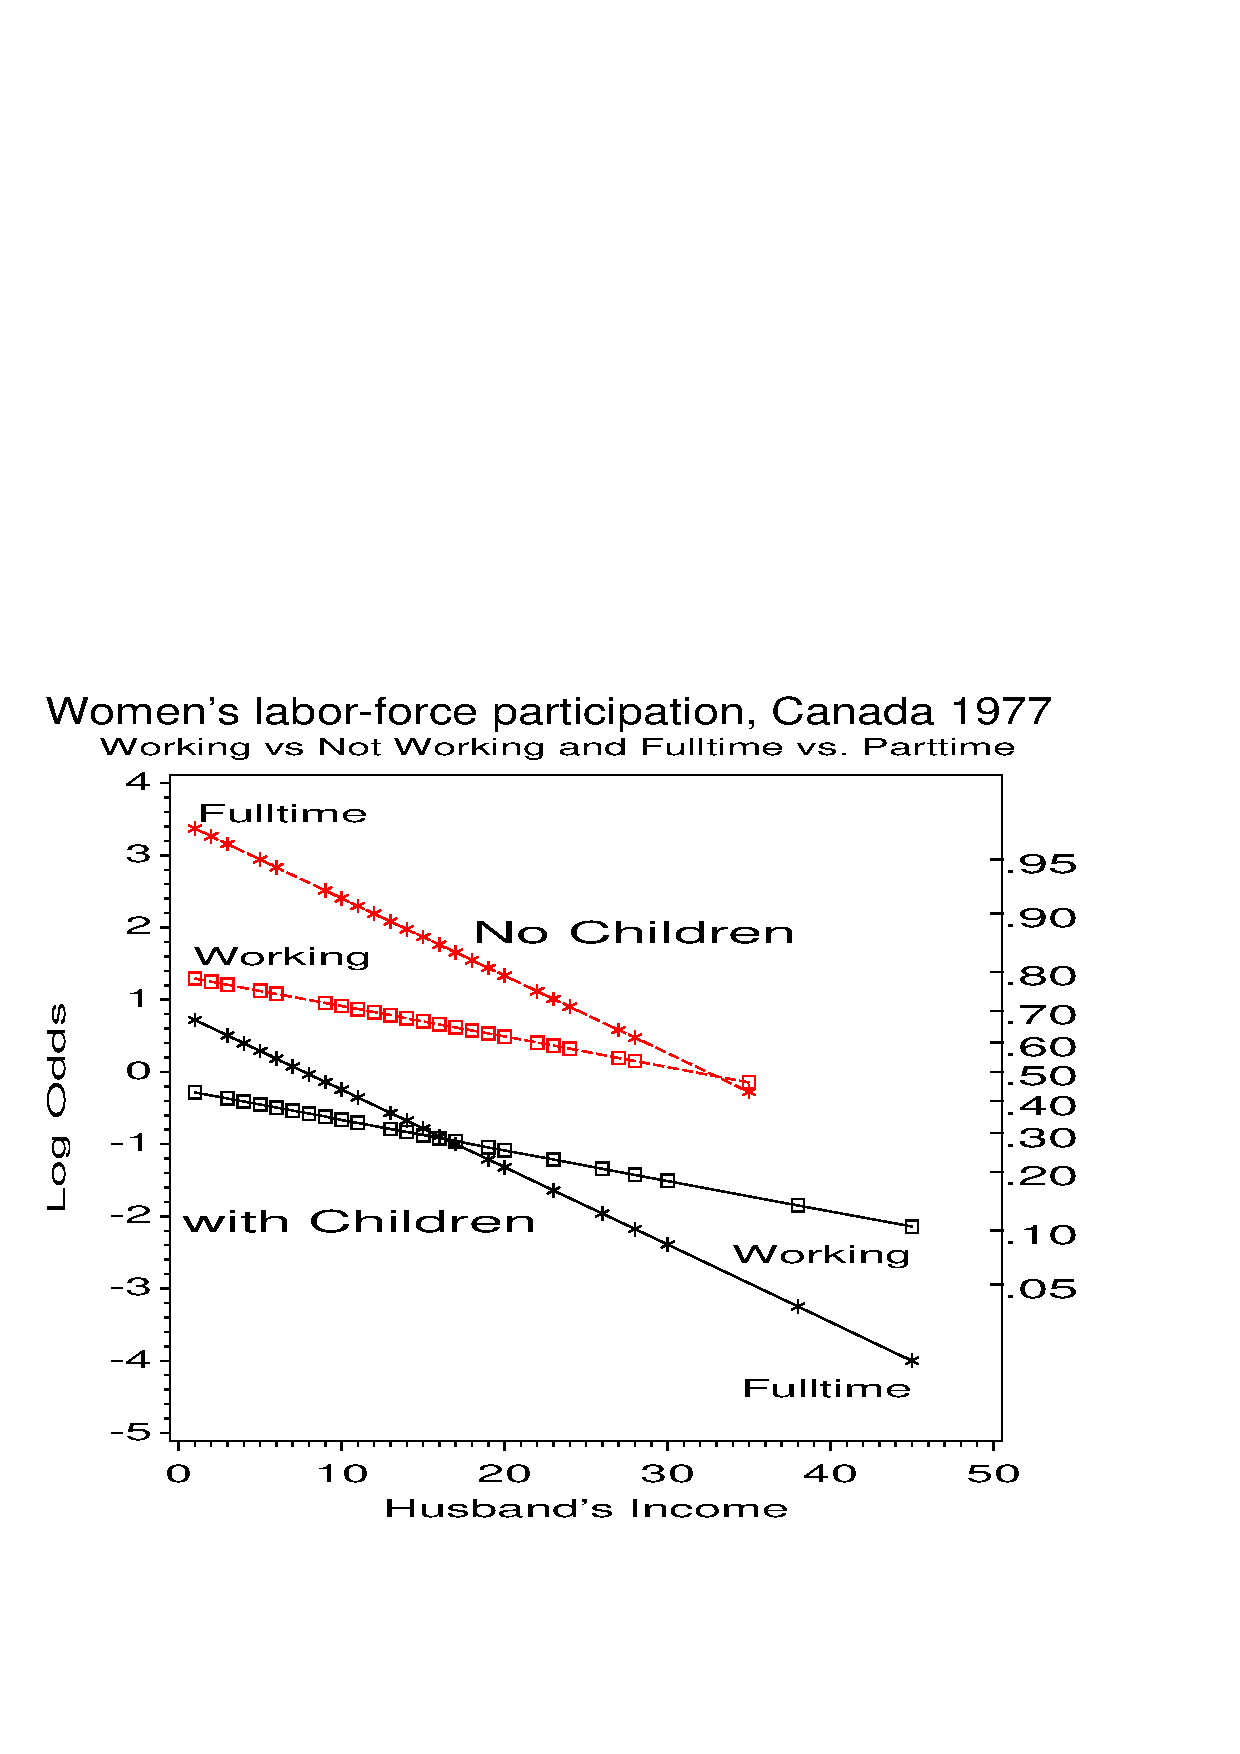
\includegraphics[scale=.7]{ch\thechapter/fig/wlfpart}
  \caption{Predicted log odds of working vs.\ not working, and of fulltime work vs.\ parttime work}\label{fig:wlfpart}
\end{figure}

To construct this graph, first join the separate results \Dsets\
into one.

\begin{listing}
*-- Merge the results to create one plot;
data both;
   set resultw(in=inw)
       resultf(in=inf);
   if inw then do;
      if children=1 then event='Working, with Children ';
      else event='Working, no Children ';
   end;
   else do;
      if children=1 then event='Fulltime, with Children ';
      else event='Fulltime, no Children ';
  end;
\end{listing}

Then, we can plot the log odds (or predicted probability) against
husband's income, using \pname{event} as to determine the curves to be
joined and labeled.
(The probability scale is constructed with the \macro{PSCALE}, and the
labels with an \ADS.  These steps are not similar to those described
in \exref{ex:arthrit10} and are
shown here).

\begin{listing}
proc gplot data=both;
   plot logit * husinc = event /
        anno=lbl nolegend frame vaxis=axis1;
   axis1 label=(a=90 'Log Odds') order=(-5 to 4);
   title2 'Working vs Not Working and Fulltime vs. Parttime';
   symbol1 v=dot    h=1.5 i=join l=3 c=red;
   symbol2 v=dot    h=1.5 i=join l=1 c=black;
   symbol3 v=circle h=1.5 i=join l=3 c=red;
   symbol4 v=circle h=1.5 i=join l=1 c=black;
\end{listing}
\end{Example}

\renewcommand{\FileName}{genlogit}
% slide template
\subsection{Basic ideas}
\begin{frame}
  \frametitle{Polytomous response: Generalized Logits}
  \begin{itemize}
	\item Models the probabilities of the $m$ response categories 
	as \(m - 1\) logits comparing
each of the first \(m - 1\) categories to the last (reference) category.
	\item Logits for any  pair of categories can be calculated
from the \(m - 1\) fitted ones.
	\item With $k$ predictors, \(x_1, x_2, \dots , x_k\), for $j=1, 2, \dots ,
	  m-1$, 
\begin{eqnarray*}
  L_{jm}  \equiv 
    \log \left( \frac{\pi_{ij}}{\pi_{im}} \right) & = & \beta_{0j}  +
  \beta _{1j} \,  x_{i1}  +
  \beta _{2j} \,  x_{i2}  + \cdots +
  \beta _{kj} \,  x_{ik} \quad \\
%  \mbox{for } j=1, 2, \dots , m-1 \\
  & = & \vec{\beta}_j \trans \vec{x}_i
\end{eqnarray*}

      \begin{itemize*}
	  \item One set of fitted coefficients, $\vec{\beta}_j$ for each
response category except the last.
	  \item Each coefficient, $\beta_{hj}$, gives the effect on the log odds
of a unit change in the predictor $x_h$
that an observation belongs to category $j$ vs.\ category $m$.
	  \end{itemize*}
	\item Probabilities in response caegories are calculated as:
\begin{equation*}
\pi_{ij} =
 \frac{ \exp ( \vec{\beta}_j \trans \vec{x}_i ) }
      { \sum_{j=1}^{m-1} \exp ( \vec{\beta}_j \trans \vec{x}_i ) }
	  \comma \, j=1,\dots, m-1 \,;
	  \quad\quad \pi_{im} = 1 - \sum_{j=1}^{m-1} \pi_{ij}
\end{equation*}
  \end{itemize}
\end{frame}

\begin{frame}[fragile]
  \frametitle{Polytomous response: Generalized Logits}
Fitting generalized logit models with SAS:
%  \begin{itemize}
%	\item SAS:
      \begin{itemize*}
	  \item Use \PROC{LOGISTIC} with \texttt{LINK=GLOGIT} option.
    	\begin{itemize*}
		\item \ODS\ $\rightarrow$ fitted probabilities, $\widehat{\pi}_{ij}$ for all $m$ categories
		\item Overall tests and specific tests for each predictor, for all $m$ categories
		\end{itemize*}
\vspace{2ex}
\begin{Input}[numbers=none]
proc logistic data=wlfpart;
   model labor = husinc children / \sasemph{link=glogit};
   output out=results p=predict xbeta=logit;
\end{Input}
	  \item Can also use \PROC{CATMOD} with \texttt{RESPONSE=LOGITS} statement.
    	\begin{itemize*}
		\item Same model, same predicted probabilities
		\item Different syntax, \ODS\ format, plotting steps
		\item Quantitative variables: \alert{\texttt{direct}} statement
		\end{itemize*}
\vspace{2ex}
\begin{Input}[numbers=none]
proc catmod data=wlfpart;
   \sasemph{direct husinc;}
   model labor = husinc children;
   \sasemph{response logits} / out=results;
\end{Input}
	  \end{itemize*} 

%  \end{itemize}
\end{frame}

\begin{frame}<1>[label=wlfpart5g]
  \frametitle{Example: Women's Labour Force Participation}
Graphs:
% two figures 
 \begin{minipage}[b]{.5\linewidth}
  \centering
  \includegraphics[width=.99\linewidth]{fig/wlfpart51}
 \end{minipage}%
 \begin{minipage}[b]{.5\linewidth}
  \centering
  \includegraphics[width=.99\linewidth]{fig/wlfpart52}
 \end{minipage}
\end{frame}


\begin{frame}[fragile]
  \frametitle{Example: Women's Labour Force Participation}
\begin{Input}[label=\fbox{\texttt{wlfpart5.sas} $\cdots$}]
title 'Generalized logit model';
proc logistic data=wlfpart;
   model labor = husinc children / \sasemph{link=glogit};
   \sasemph{output out=results p=predict xbeta=logit;}
\end{Input}
Response profile:
\begin{Output}[gobble=7]
                       Ordered                      Total
                         Value        labor     Frequency

                             1            1            66
                             2            2            42
                             3            3           155

             Logits modeled use labor=3 as the reference category.
\end{Output}
\emph{Note:} Not working is the baseline category
\end{frame}


\begin{frame}[fragile]
Overall and Type III tests:
\begin{Output}[gobble=7,baselinestretch=0.8]
                    Testing Global Null Hypothesis: BETA=0
 
            Test                 Chi-Square       DF     Pr > ChiSq

            Likelihood Ratio        77.6106        4         <.0001
            Score                   76.4850        4         <.0001
            Wald                    58.4351        4         <.0001

                          Type III Analysis of Effects
 
                                            Wald
                  Effect        DF    Chi-Square    Pr > ChiSq

                  husinc         2       12.8159        0.0016
                  children       2       53.9806        <.0001
\end{Output}
These are comparable to the combined tests for the nested dichotomies models.
\end{frame}

\begin{frame}[fragile]
Coefficients:
\begin{Output}[gobble=2,baselinestretch=0.8, fontsize=\footnotesize]
                    Analysis of Maximum Likelihood Estimates
 
                                          Standard          Wald
  Parameter    labor    DF    Estimate       Error    Chi-Square    Pr > ChiSq

  Intercept    1         1      1.9828      0.4842       16.7709        <.0001
  Intercept    2         1     -1.4323      0.5925        5.8445        0.0156
  husinc       1         1     -0.0972      0.0281       11.9762        0.0005
  husinc       2         1     0.00689      0.0235        0.0863        0.7689
  children     1         1     -2.5586      0.3622       49.9008        <.0001
  children     2         1      0.0215      0.4690        0.0021        0.9635
\end{Output}
i.e., the fitted models are:
\begin{eqnarray*}
  \log \left( \frac{ \Pr ( \mbox{fulltime} ) }
  { \Pr ( \mbox{not working} ) } \right) & = &
  1.983 - 0.097 \,  \mbox{H\$} - 2.56 \,  \mbox{kids} \\  %\label{eq:wlfgen1}
%
  \log \left( \frac{ \Pr ( \mbox{parttime} ) }
  { \Pr ( \mbox{not working} ) } \right) & = &
  -1.432 - 0.0069 \,  \mbox{H\$} - 0.0215 \,  \mbox{kids}  % \label{eq:wlfgen2}
\end{eqnarray*}
\emph{Interpretation:} Signs for \texttt{husinc} and \texttt{children} are understandable,
but need to make a plot!
\end{frame}

\begin{frame}[fragile]
\ODS\ \texttt{results} (for plots):
\begin{Output}[baselinestretch=0.7,gobble=2]
  case   labor   husinc  children   _LEVEL_     logit    predict

    1      3       15        1         1      -2.03423   0.09333
    1      3       15        1         2      -1.30743   0.19305
    1      3       15        1         3        .        0.71363
    2      3       13        1         1      -1.83977   0.11142
    2      3       13        1         2      -1.32122   0.18715
    2      3       13        1         3        .        0.70143
    3      3       45        1         1      -4.95114   0.00528
    3      3       45        1         2      -1.10067   0.24830
    3      3       45        1         3        .        0.74642
    4      3       23        1         1      -2.81207   0.04464
    4      3       23        1         2      -1.25230   0.21238
    4      3       23        1         3        .        0.74298
    5      3       19        1         1      -2.42315   0.06486
    5      3       19        1         2      -1.27987   0.20346
    5      3       19        1         3        .        0.73168
    6      3        7        1         1      -1.25639   0.18478
    6      3        7        1         2      -1.36257   0.16616
    ...
\end{Output}
\begin{itemize*}
	\item \texttt{logit} gives the two fitted log odds vs Not working
	\item \texttt{predict} gives the predicted probability for each category of \texttt{labor}
\end{itemize*}
\end{frame}

\begin{frame}[fragile]
  \frametitle{Example: Women's Labour Force Participation}
\begin{Input}[label=\fbox{$\cdots$ \texttt{wlfpart5.sas}},baselinestretch=0.7]
proc sort data=results;
   \sasemph{by children husinc _level_;}

   \sascomment{*-- Curve labels;}
%label(data=results, x=husinc, y=predict, cvar=_level_,
   by=children, subset=last._level_, text=put(_level_, labor.), 
   pos=2, out=labels1);

   \sascomment{*-- Panel labels;}
%label(data=results, x=20, y=0.85, 
   by=children, subset=last.children, text=put(children, kids.), 
   pos=2, size=2, out=labels2);
data labels;
   set labels1 labels2;
   by children;

goptions hby=0;
proc gplot data=results;
   \sasemph{plot predict * husinc = _level_} / 
      vaxis=axis1 hm=1 vm=1 \sasemph{anno=labels} nolegend;
   by children;
   axis1 order=(0 to .9 by .1) label=(a=90);
   symbol1 i=join v=circle   c=black;
   symbol2 i=join v=square   c=red;
   symbol3 i=join v=triangle c=blue;
   run;
\end{Input}
\end{frame}

\againframe<1>{wlfpart5g}
\endinput

% slide template
\begin{frame}
  \frametitle{}
  \begin{itemize}
	\item{\large\bfseries }
      \begin{itemize*}
	  \item 
    	\begin{itemize*}
		\item 
		\item 
		\end{itemize*}
	  \item 
	  \end{itemize*}
	\item{\large\bfseries }
	\item{\large\bfseries }
  \end{itemize}
\end{frame}



\section{The Bradley-Terry-Luce Model for Paired Comparisons}\label{sec:logist-btl}
The basic methodology of logistic regression finds application in
a surprising variety of applications
\citep{Strauss:92}.
One example is a model for paired comparisons data proposed by
\citet{BradleyTerry:52}, and by \citet{Luce:59} in a more general context.
In paired comparisons, $K$ objects are compared in a pairwise manner
and the goal is to determine scale values and a ranking of these objects.
For example, a market researcher might wish to construct a preference ranking for
soft drinks among consumers.  In other contexts, the objects might be
teams or players in a sports league, or sounds of varying intensity
or frequency to be judged in a psychophysical experiment.

The Bradley-Terry-Luce (BTL) model assumes that, for each object there is
a parameter, $\theta_i$, such that the probability of the event $(i > j)$
that object $i$
is preferred to object $j$ is
\begin{equation}\label{eq:btl1}
\Pr ( i > j ) = \frac{\theta_i}{\theta_i + \theta_j}
\period
\end{equation}
Luce's model is more general, and $\theta_i$ is interpreted as
the probability that object $i$ is ranked first within \emph{any} subset
of objects.
The BTL model \eqref{eq:btl1} may be cast as a logit model with parameters
$\beta_i,= \log \theta_i$ as follows.
Substituting $\theta_i = \exp (\beta_i)$ in \eqref{eq:btl1} gives,
\begin{equation}\label{eq:btl2}
\Pr ( i > j ) = \frac{\exp(\beta_i)}{\exp(\beta_i) + \exp(\beta_j)}
     = \frac{1}{1 + \exp(\beta_i / \beta_j)}
	  \period
\end{equation}
But \eqref{eq:btl2} is just the inverse logit of $\theta_i/\theta_j$. Hence,
\begin{eqnarray}
\logit [ \Pr (i>j)] = \log \left( \frac{\Pr (i>j)}{\Pr (j>i)} \right)
    & = & \beta_i - \beta_j  \label{eq:btl3} \\
    & = & \vec{x}\trans \vec{\beta} \nonumber
\end{eqnarray}
where, $\vec{\beta} = ( \beta_1, \dots , \beta_K)\trans$ and
$\vec{x} = \{x_k\}$ is a vector with
$x_k = 1$ if $k=i$, $x_k = -1$ if $k=j$, and 0 otherwise.
Thus, model \eqref{eq:btl3} is a logit model with no intercept,
and with a $K (K-1)/2 \times K$ matrix $\mat{X}$ of explanatory
variables whose rows give the items compared in each
paired comparison.  For $K=4$ objects, for example, the $\mat{X}$ matrix is
\begin{equation*}
 \mat{X} = \left[
  \begin{array}{rrrr}
  1 & -1 & 0 & 0 \\
  1 & 0 & -1 & 0 \\
  1 & 0 & 0 & -1 \\
  0 & 1 & -1 & 0 \\
  0 & 1 & 0 & -1 \\
  0 & 0 & 1 & -1 \\
  \end{array}
 \right]
 \period
\end{equation*}

The model assumes that all comparisons are independent.  In particular,
when items are rated by different judges,  the ratings of different
pairs by the same judge must also be independent, and all judges are
assumed homogeneous.
More general versions of the BTL model, allowing subject-specific
covariates, are described by \citet{Dittrich-etal:1998}.

\begin{Example}[winloss]{1987 baseball standings}
\tabref{tab:winloss} (from \citet[p. 372]{Agresti:90}) shows the
final results from the 1987 baseball season for the teams in the Eastern Division
of the American League.
Each team played every other team a total of $n_{ij} = 13$ times,
so (assuming that the outcome of each game is independent)
we may regard the values in the lower triangle
as binomial observations, $\Bin( \pi_{ij}, 13 )$.
\begin{table}[htb]
 \caption{1987 American League Baseball Results}\label{tab:winloss}
 \begin{center}
 \begin{tabular}{l| rrrrrrr}
 \hline
 Winning & \multicolumn{7}{c}{Losing Team} \\ \cline{2-8}
 Team    & Mil & Det & Tor & NY & Bos & Cle & Bal \\
 \hline
Milwaukee & $-$ &  7  &  9  &  7  &  7  &  9  & 11 \\ 
Detroit   &  6  & $-$ &  7  &  5  & 11  &  9  &  9 \\ 
Toronto   &  4  & 6   & $-$ &  7  &  7  &  8  & 12 \\ 
New York  &  6  & 8   &  6  & $-$ &  6  &  7  & 10 \\ 
Boston    &  6  & 2   &  6  &  7  & $-$ &  7  & 12 \\ 
Cleveland &  4  & 4   &  5  &  6  &  6  & $-$ &  6 \\ 
Baltimore &  2  & 4   &  1  &  3  &  1  &  7  & $-$ \\ 
 \hline
 \end{tabular}
 \end{center}
\end{table}


We concentrate here on fitting the BTL model and graphical displays of
the scale values and model diagnostics.
A similar example, without graphs, is given in
\emph{Logistic Regression Examples Using the SAS System}, Example 19.

The first \Dstp\ below reads the complete data from \tabref{tab:winloss}.
In a second step, variables in the array \pname{X} are created, corresponding
to the model matrix in \eqref{eq:btl3}.
The resulting \Dset, \pname{winloss2} is shown in \outref{out:btl2.1}.
%% input: /Users/friendly/sasuser/catdata/btl2.sas
%% last modified: 29-Jul-99  9:21
\begin{listing}
title 'Bradley-Terry-Luce Model, 1987 American League, East';
data winloss;
  input t1-t7;
  games=13;
datalines;
  .  7  9  7  7  9 11
  6  .  7  5 11  9  9
  4  6  .  7  7  8 12
  6  8  6  .  6  7 10
  6  2  6  7  .  7 12
  4  4  5  6  6  .  6
  2  4  1  3  1  7  .
;
data winloss2;
   retain i 0 ;
   array team\{*\} t1-t7;
   array x\{*\} milwauke detroit toronto new_york boston clevelan baltimor;
   retain milwauke detroit toronto new_york boston clevelan baltimor 0;
   set winloss;
   names='Milwaukee Detroit Toronto New_York Boston Cleveland Baltimore';
   length winner loser $9;
   i+1;
   do j=1 to dim(team);
      if team\{j\} ne . then do;
         count=team\{j\};
         x\{i\}=1;
         x\{j\}=-1;
         winner = scan(names,i);
         loser  = scan(names,j);
         if i < j then output;
         x\{i\}=0;
         x\{j\}=0;
      end;
   end;
   drop i j t1-t7 names;
\end{listing}


\begin{Output}[!htb]
\caption{Win-loss data, set up for fitting BTL model with \PROC{LOGISTIC}}\label{out:btl2.1}
\small
\verbatiminput{ch6/out/btl2.1}
\end{Output}
The BTL model is fit using the \PROC{LOGISTIC} step below.
The options \pname{OUTEST} and \pname{COVOUT} create an \ODS\
containing the estimated $\beta_i$ parameters and their
variance-covariance matrix.
A second \ODS\ containing fitted probabilities and model diagnostic
measures is created with the \stmt{OUTPUT}{LOGISTIC}.
The parameters and their standard errors are shown in \outref{out:btl2.2}.
Thus, according to the BTL model \eqref{eq:btl1},
the predicted probability that Toronto beats Cleveland would be
$\exp(1.294)/(\exp(1.294) + \exp(0.684)) = 0.648$.
The squared standard errors are contained along the diagonal of the
variance-covariance matrix in the \pname{PARM1} \Dset.
A small \IML\ step is used to extract the parameter estimates and
standard errors.
%% input: /users/faculty/friendly/sasuser/catdata/btl2.sas
%% last modified: 15-Sep-98 11:29
\begin{listing}
proc logistic data=winloss2 nosimple out=parm1 covout;
  model count/games=milwauke detroit toronto new_york
                    boston clevelan baltimor / noint;
  output out=fit prob=prob resdev=resdev c=c;
run;

*-- Extract parameters and standard errors;
proc iml;
   use parm1;
   read all var \{_name_\} into name where(_type_='COV');
   read all var \{milwauke detroit toronto new_york
                 boston clevelan baltimor\} into parm where(_type_='PARMS');
   read all var \{milwauke detroit toronto new_york
                 boston clevelan baltimor\} into cov where(_type_='COV');

   stderr = exp(sqrt(vecdiag(cov)));
   parm = exp(t(parm));
   create parms var \{name parm stderr\};
   append var \{name parm stderr\};

proc rank data=parms out=parms descending;
   var parm;
   ranks rank;
   label parm='Scale Value'
      rank='Team Rank';
\end{listing}

\begin{Output}[htb]
\caption{Win-loss data, \PROC{LOGISTIC} output}\label{out:btl2.2}
\small
\verbatiminput{ch6/out/btl2.2}
\end{Output}

%% one figure
\begin{figure}[!htb]
  \centering
  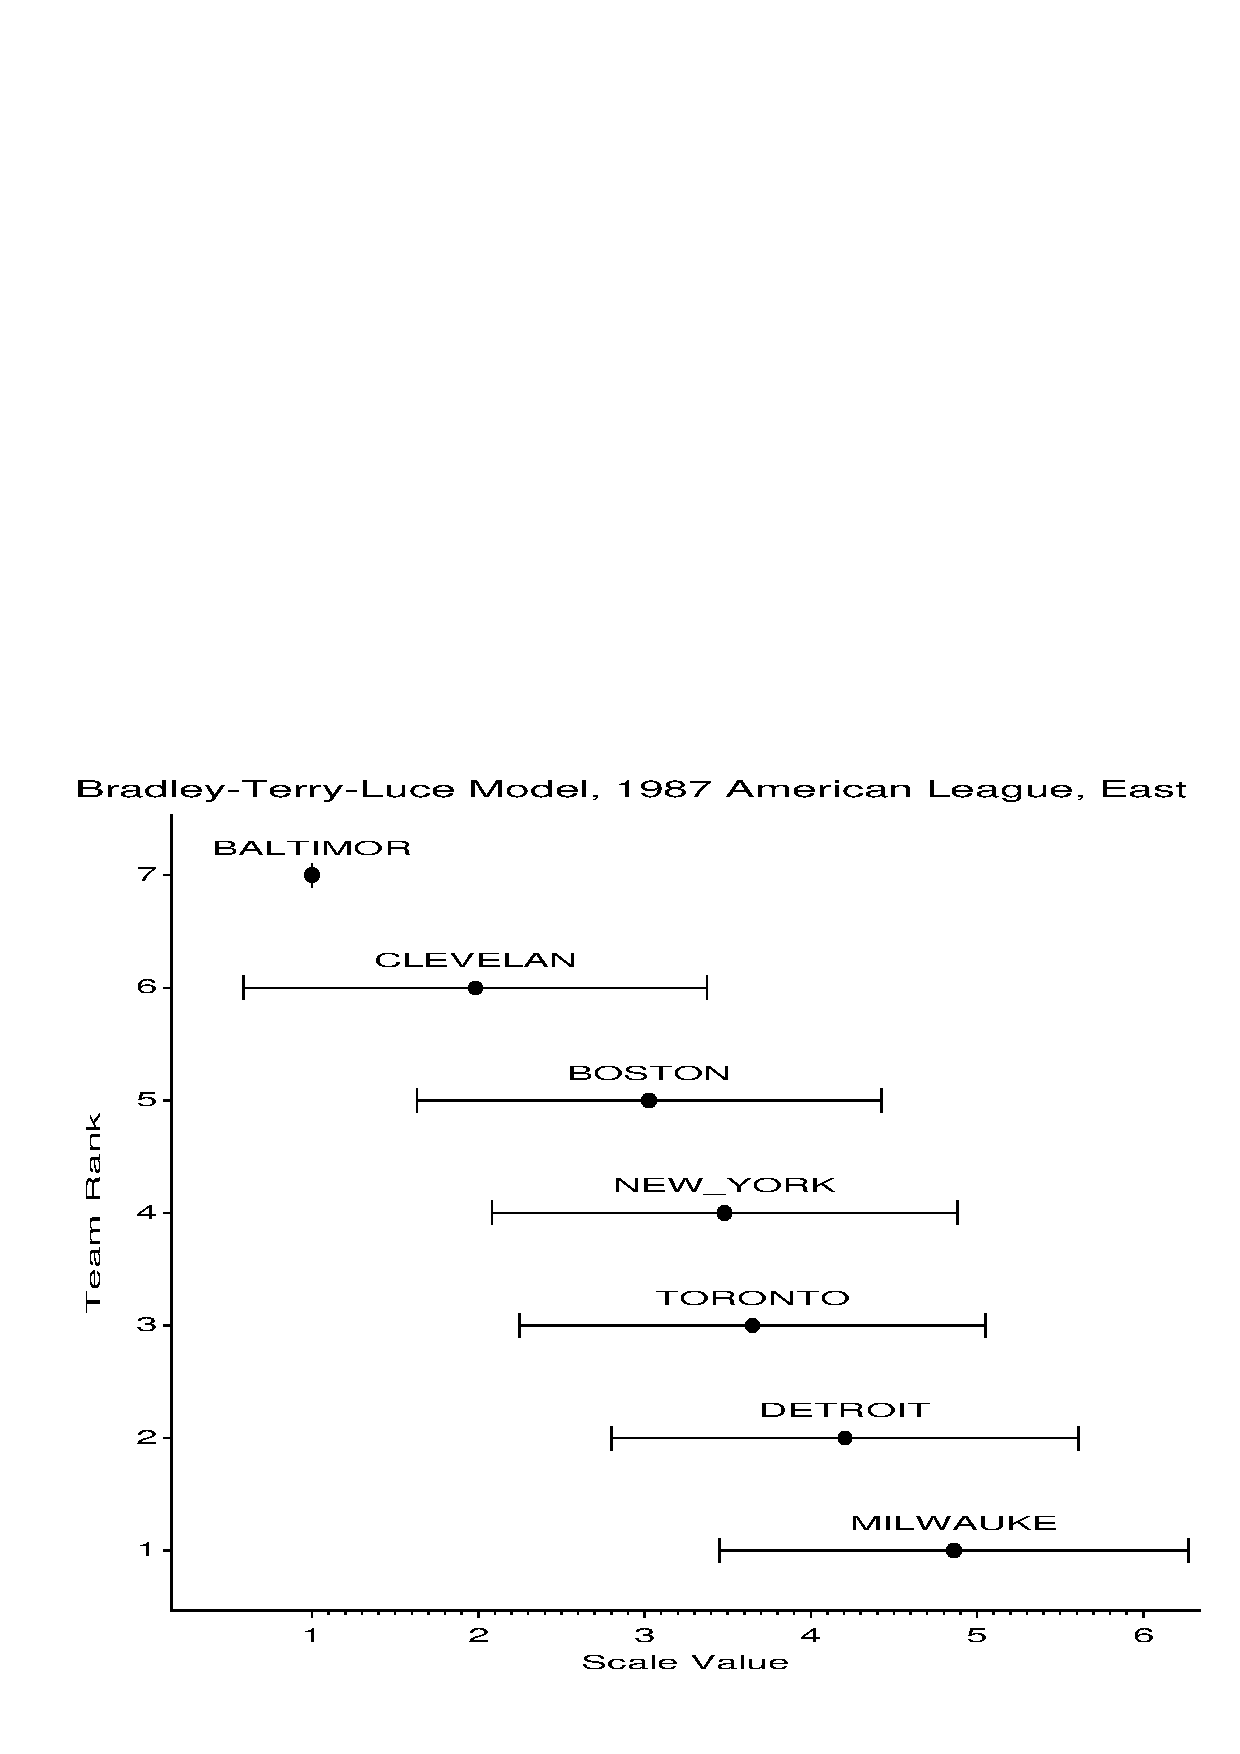
\includegraphics[scale=.6]{ch6/fig/btl21}
  \caption{Scale values and standard errors for 1987 baseball data}%
  \label{fig:btl21}
\end{figure}
The plot of scale values and standard errors shown in \figref{fig:btl21}
is produced by the first \PROC{GPLOT} step below.
The \macro{BARS} constructs the \ADS\ to draw the standard error bars,
and the \macro{LABEL} produces the team label annotations.
%% input: /users/faculty/friendly/sasuser/catdata/btl2.sas
%% last modified: 15-Sep-98 11:29
\begin{listing}
%bars(data=parms, var=parm, class=rank, barlen=stderr, baxis=x, barwidth=.1);
%label(data=parms, x=parm, y=rank, text=name, pos=2, yoff=.1, out=_lab_);
data _bars_;
   set _bars_ _lab_;

proc gplot data=parms;
   plot rank * parm / 
      anno=_bars_ vaxis=axis1 haxis=axis2 vm=0;
   symbol v=dot color=black h=1.6;
   axis1 label=(a=90) offset=(5);
    axis2 order=(1 to 6) offset=(10,4);
run; quit;

%label(data=fit, x=prob, y=resdev, out=_lab_,
   subset=%str(abs(resdev)>.9),
   text = %str(substr(winner,1,3) || '>' || substr(loser,1,3)));
title;
proc gplot data=fit;
   bubble resdev * prob = c /
      anno=_lab_ bsize=20 bcolor=gray80 vaxis=axis1 vm=1;
   axis1 label=(a=90);
   label prob = 'Estimated Winning Probability';
\end{listing}


%% one figure
\begin{figure}[htb]
  \centering
  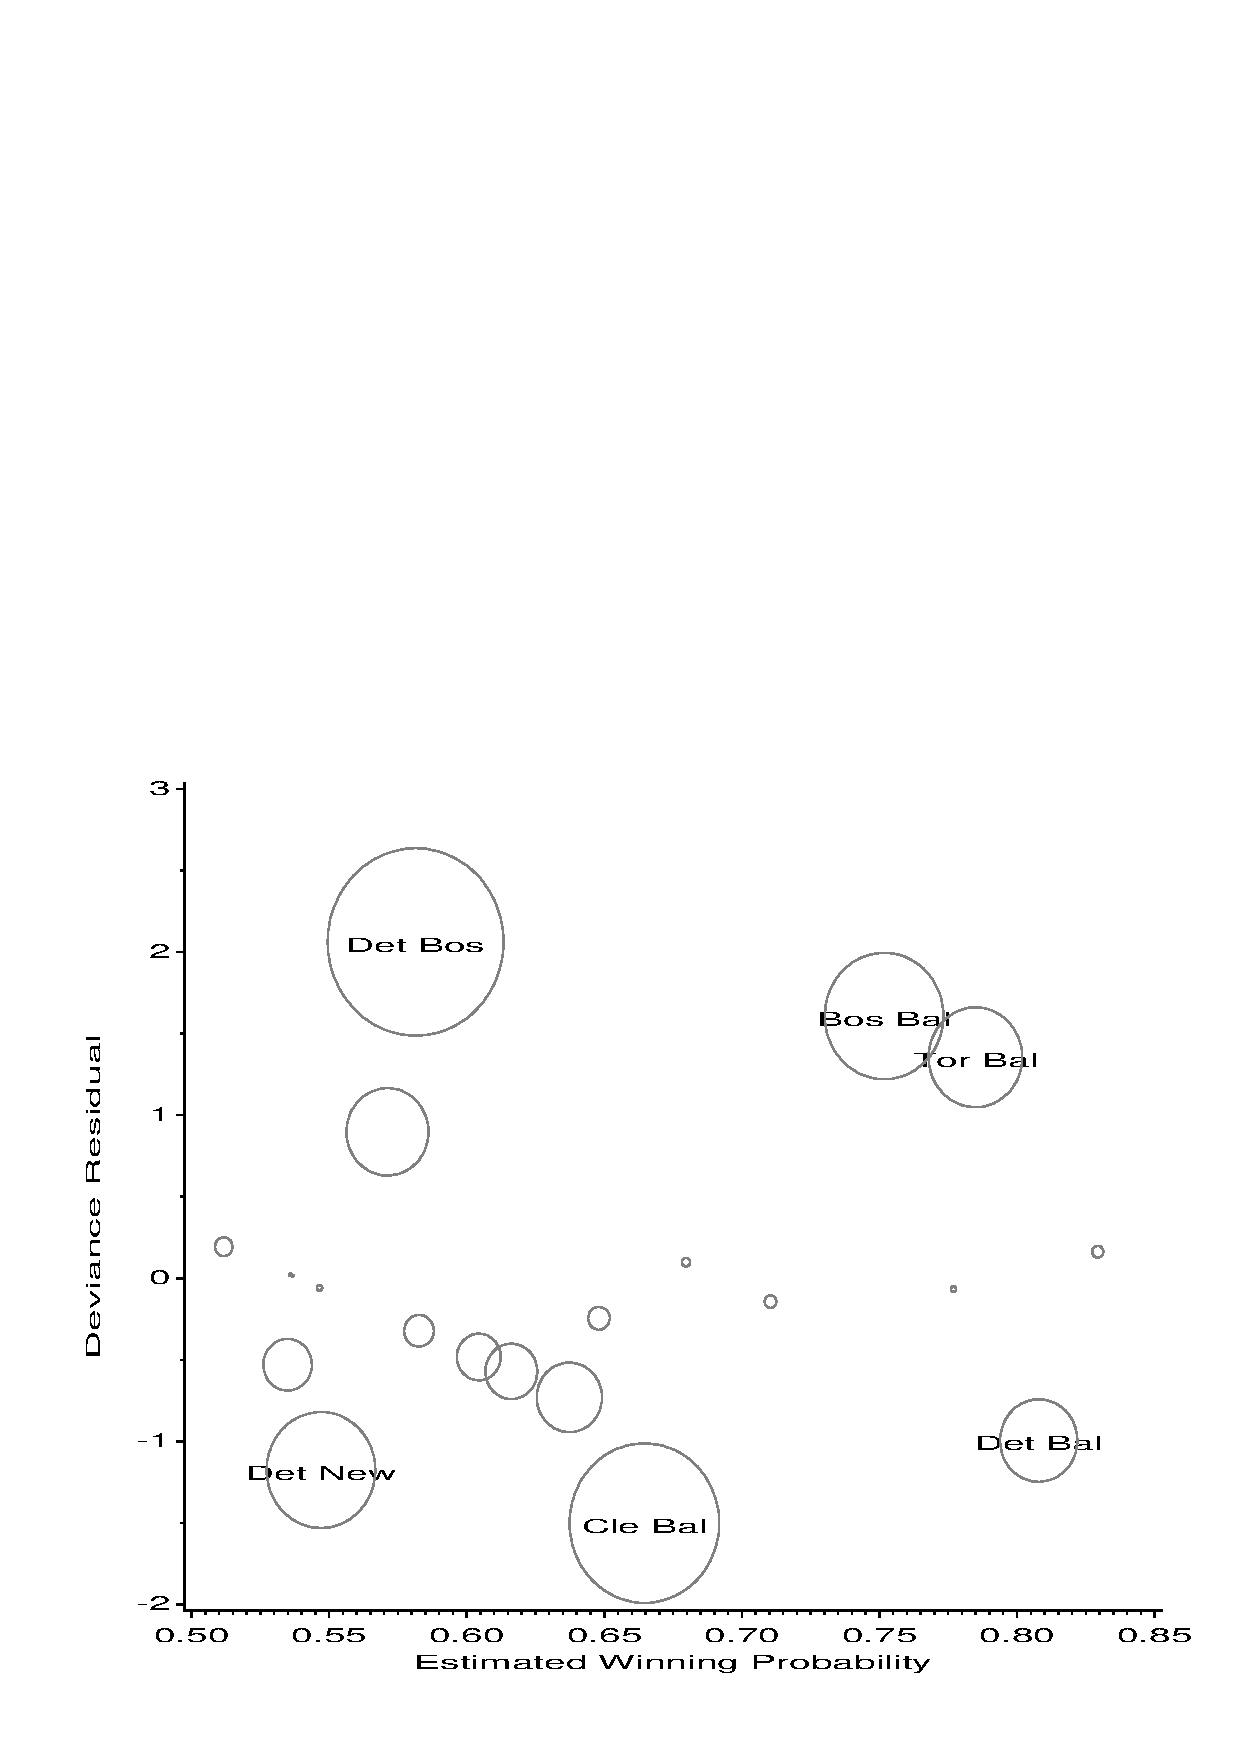
\includegraphics[scale=.6]{ch6/fig/btl22}
  \caption{Diagnostic plot for 1987 baseball data}%
  \label{fig:btl22}
\end{figure}
The diagnostic plot shown in \figref{fig:btl22} plots the deviance residual
against predicted probabilities.  The bubble size is proportional to Cook's
distance, $C_i$.  Only one observation has a residual (slightly) greater than 2,
and no $C_i$ are excessive, so the BTL model seems to provide a reasonable
fit.
\end{Example}

\section{Power and sample size for logistic regression} \label{sec:logistic-power}

The goal of many studies is to determine if a given predictor $X$ has
an effect on a binary outcome variable.
In planning such studies it is often crucial to determine the sample
size required in order to have a reasonable chance to detect an effect
of a given size.  Alternatively, if a study failed to detect a significant
effect, we might wish to determine if no real effect is present, or if
the sample size in the study was just insufficient to detect it.

In either case, power and sample size determination requires that we specify the Type I error rate, $\alpha$, of the test, and the \glossterm{effect size}
we wish to detect.  In the simple logistic model with one predictor,
\begin{equation*}
 \log \frac{\pi}{1-\pi} = \beta_0 + \beta_1 X
 \comma
\end{equation*}
the null hypothesis is $H_0 : \beta_1 = 0$, and the size of the effect
depends directly on the magnitude of the slope $\beta_1$.
That is, power increases with $| \beta_1 |$;  correspondingly, the sample
size required to detect an effect of given size (i.e., reject $H_0$ at
a given $\alpha$-level)
decreases with $| \beta_1 |$.

The difficulty in practice is that it is often difficult for the
researcher to specify the size of meaningful effect in terms of the
slope $\beta_1$ of the logistic model.
We describe below two standard situations in which effect size of interest
may be specified more simply to determine approximate power or
required sample size.

\subsection{Binary predictor: Comparing two proportions}
When there is a single binary predictor (and a binary response),
we may take $X=0$ for Group 1, and $X=1$ for Group 2,
so that $\beta_1$ is the log odds of ``success'' response in Group 2
as compared to Group 1.  

But, in this case
the data comprise a $2\times 2$ table, and the test of the logistic model
is analogous to a test of the difference of proportions in
two independent samples.  That is, $H_0 : \beta_1 = 0$ is
analogous to the test of $H_0 : \pi_1 = \pi_2$.
In this case the sample difference, $p_1 - p_1$
has an approximate large-sample normal distribution, with variance
\begin{equation*}
 \sigma_{p_1 - p_2}^2 = \frac{\pi_1 (1 - \pi_1)}{n_1} +
 \frac{\pi_2 (1 - \pi_2)}{n_2}
 \period
\end{equation*}

Assume that we are interested in being able to reject the null
hypothesis when the true difference  $|\pi_1 - \pi_2| = \pi_d$ is at least
some given value.  $\pi_1$ and $\pi_2$ (or $\pi_1$ and $\pi_d$)
provide a reasonable way to
specify the size of the effect of interest in this situation.

For example, in planning the arthritis treatment
experiment, the investigators might assume that
the probability of at least some improvement would be around $\pi_2 = 0.30$
with the placebo, and wish to have a high probability of rejecting
$H_0$ when the probability of at least some improvement with the active
treatment                                                                                                                                                     
is $\pi_1 = 0.50$
or greater.  The difference $\pi_d$ is usually the smallest difference
of substantive interest.  We also assume that $n_1 = n_2$.

Then the power of a two-tailed $\alpha$-level test of 
$H_0 : |\pi_1 - \pi_2 | = 0$
against the alternative $H_1: |\pi_1 - \pi_2| = \pi_d$
is approximately
\begin{eqnarray}
\mbox{power} & = & \Pr \left(
 \frac{ | p_1 - p_2 | - \pi_d }{ \sigma ( p_1 - p_2 ) }
 \right) \ge z_{1-\alpha/2} \nonumber \\
 & = & \Pr [ z > z_{1-\alpha /2} - \pi_d \, \sigma_{p_1 - p_2} ]
     + \Pr [ z < z_{\alpha /2} - \pi_d \, \sigma_{p_1 - p_2} ] \nonumber \\
 & = & 1- \Phi [z_{1-\alpha /2} - \pi_d \, \sigma_{p_1 - p_2}]
     + \Phi [z_{\alpha /2} - \pi_d \,  \sigma_{p_1 - p_2}] \label{eq:power2x2}
\end{eqnarray}
where $\Phi(\bullet)$ is the cumulative normal probability calculated by the
\FUNC{probnorm}.  For example, with $\alpha=0.05$, $\pi_1=0.30$,
and $\pi_2=0.50$, and a sample size of $n = n_1 + n_2 =80$, \eqref{eq:power2x2}
gives power = 0.462 when $\pi_2 = 0.50$ ($\pi_d = 0.20$)
and power =  0.807 when $\pi_2 = 0.60$ ($\pi_d = 0.30$).

It is often more convenient to find the sample size required for a
given power.  Using $\beta = 1- \mbox{power}$ as the probability of
a Type II error,%
\footnote{Don't confuse $\beta = 1- \mbox{power}$ here with the slope, $\beta_1$,
and intercept, $\beta_0$ of the logistic regression model.  Both uses
are conventional, and there are only a limited number of Greek letters
to go around.}
the approximate sample size required may be calculated as
\begin{equation}\label{eq:nbinlog}
n_1 = n_2 = \frac{ (z_{1-\alpha /2} + z_\beta) ^2 [ \pi_1 (1-\pi_1) + \pi_2 (1-\pi_2) ]} { (\pi_1 - \pi_2)^2 }
\end{equation}

These calculations (\eqref{eq:power2x2} and
\eqref{eq:nbinlog}),
along with tabular and graphical displays of power vs.\ $n$, are performed by the \macro{POWER2X2},
described in \macref{mac:power2x2}.
The tabular display is more useful for finding the exact calculated value,
while the graphs, as usual, show the overall behavior better.

\begin{Example}[arthrit13]{Arthritis treatment}
For the arthritis treatment data, we can perform a power analysis
for $\pi_1 = 0.30$ and $\pi_d = 0.2 \,(0.1)\, 0.4$ with the following
statement:
\begin{listing}
%power2x2(p1=.30, diff=.2 to .4 by .1, plot=power * n=diff);
\end{listing}
By default, the program calculates power for a range of sample sizes,
typically 10--200, though any range may be specified with the
\mparm{NMIN}{POWER2X2} and the \mparm{NMAX}{POWER2X2}.

In addition to printed output (not shown), the macro produces a 
graph of power against total sample size ($n = n_1 + n_2$)
shown in \figref{fig:power2x2a}.
For a desired power of $1-\beta$ = 0.80, the required total
sample size is about 80--85 when $\pi_d = 0.3$, but only
about 45--50 when $\pi_d = 0.3$.
In the data, $p_1 = 28/41 = 0.683$ and $p_2 = 14/43 = 0.325$,
so with $n=83$ there was adequate power.
%% one figure
\begin{figure}[htb]
  \centering
  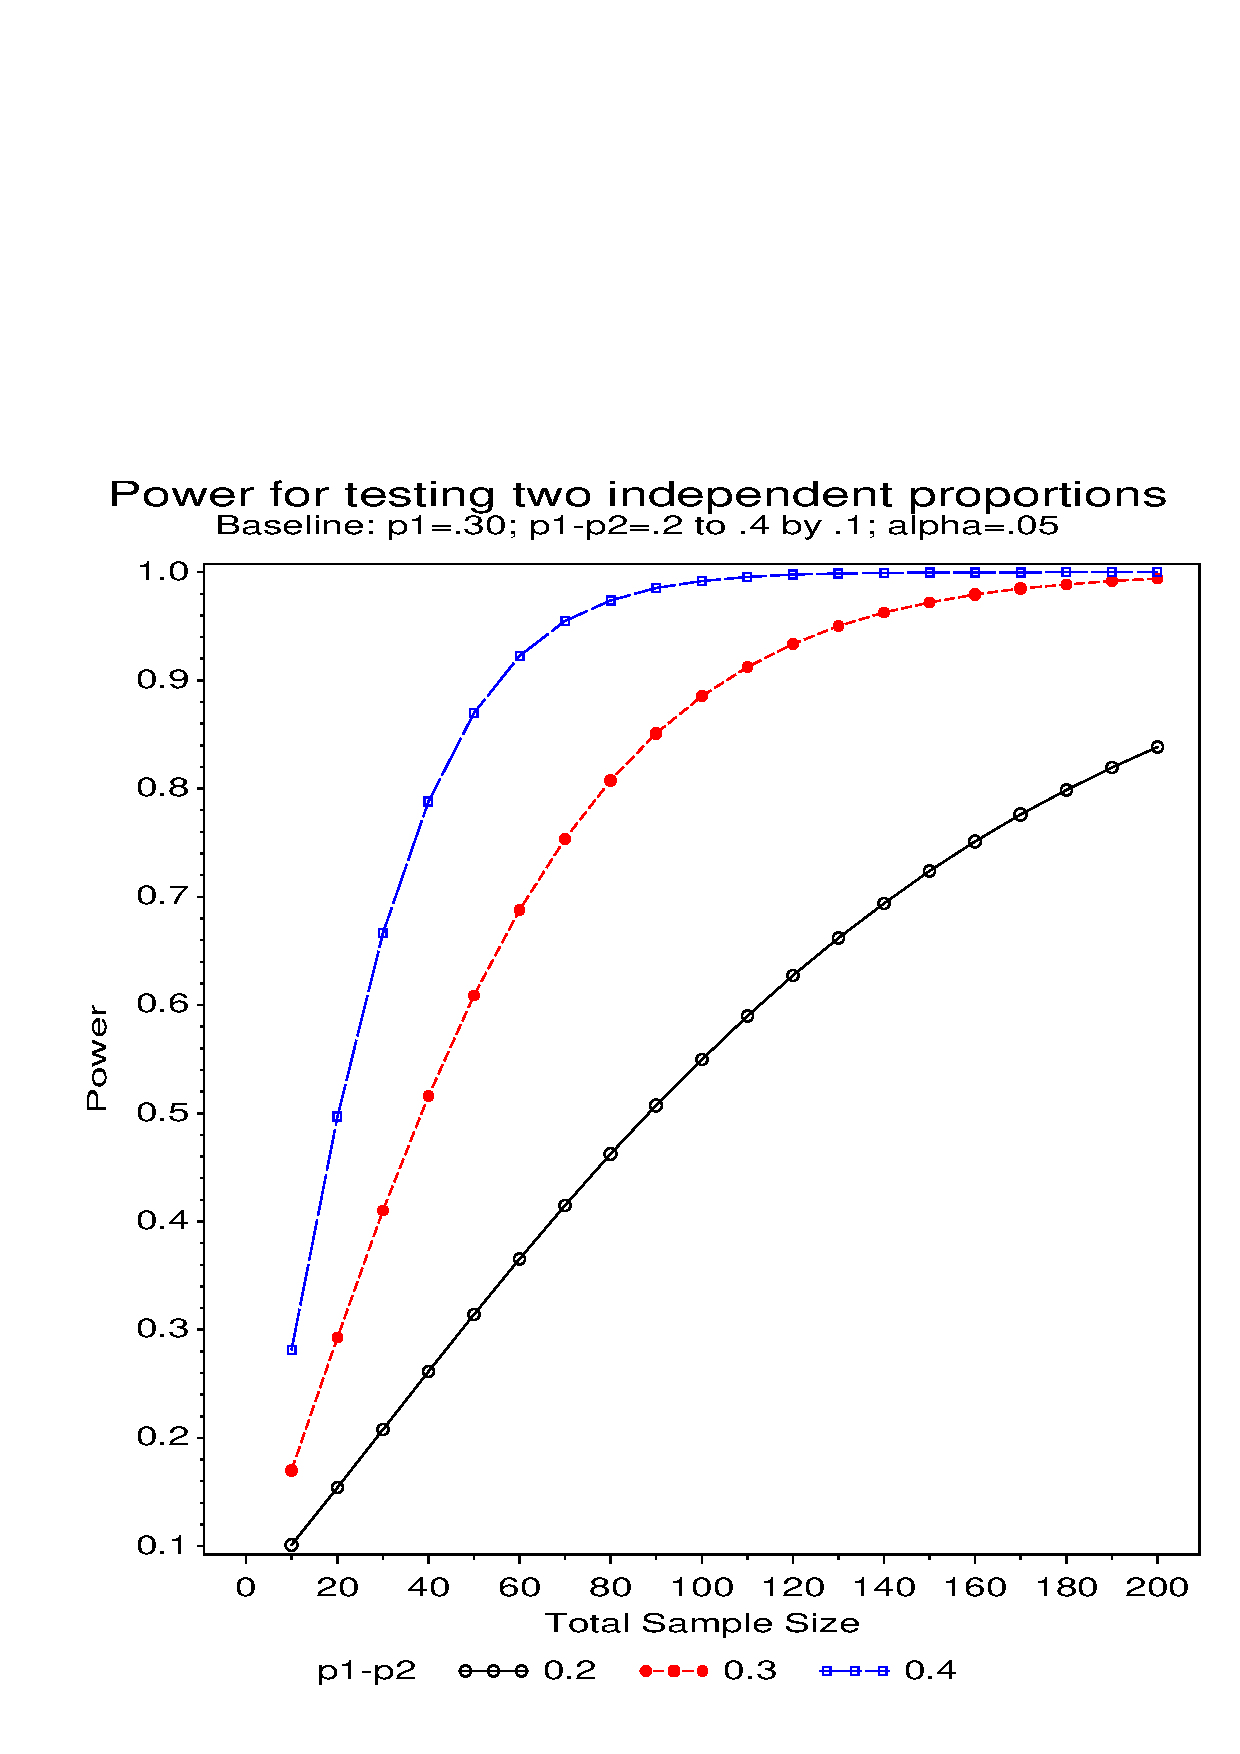
\includegraphics[scale=.6]{ch6/fig/power2x2a}
  \caption{Power analysis for arthritis treatment data}%
  \label{fig:power2x2a}
\end{figure}
\end{Example}

\subsection{Quantitative predictor}
When the predictor is quantitative, 
a simple method to specify the size of the
effect of interest is given by \citet[p. 131]{Agresti:96}
based on \citet{Hsieh:89}.
The slope $\beta_1$ under an alternative hypothesis
may be given in terms of the probabilities, $\pi_1$
and $\pi_2$ at two points, corresponding to
$X = \bar{X}$ and $X = \bar{X} + 1\mbox{s.d.}$
From these values, the effect size
can be specified in terms of the the odds ratio, 
$\theta = (p_2/(1-p_2)) \div (p_1/(1-p_1))$.

Letting $\psi = \log ( \theta )$,  Hseih provides the following
formula for the approximate sample size, $n$ required for a
one-tailed test with Type I error rate $\alpha$ and power $=1-\beta$:
\begin{equation}\label{eq:powerlog}
n = \frac{[z_{\alpha} + z_{\beta} \exp( -\psi^2 /4) ]^2 (1 + 2 p_1 \delta )} { p_1 \psi^2}
\end{equation}
where 
\begin{equation*}
\delta = \frac{1 + (1 + \psi^2) \exp( 5 \psi^2 /4) } {1 + \exp( -\psi^2 /4) }
\end{equation*}

In multiple logistic regression, larger sample sizes are required to
detect the \emph{partial} effect of one variable to the extent that
this variable is correlated with other explanatory variables
(because holding the other variables fixed then removes some of the
effect of the variable of interest).
If $R^2$ is the squared multiple correlation of the target predictor
with other predictors in the model, the unique variance of the
target variable is $1-R^2$.
To use formula \eqref{eq:powerlog} in this situation, let
$p_1$ refer to the probability of the event at the mean level of all
predictors, and divide the result of \eqref{eq:powerlog}
by $1-R^2$.
A more comprehensive approach to power analysis for 
logistic regression with multiple
covariates is described by \citet{Whittemore:81}.

These calculations are carried out by the \macro{POWERLOG},
described in \macref{mac:powerlog}.
The values of the input parameters
\pname{P1}, \pname{P2}, \pname{ALPHA}, \pname{POWER}, and \pname{RSQ},
may be supplied as macro arguments, or as variable values in an
input \Dset.
Output includes both a table and a graphical display.
\begin{Example}[power1]{Power for one or more predictors}
The following statement calculates the power of a test for $X_1$
when the probability of the event at $X = \bar{X}$ is $p_1 = 0.50$
and the probability of the event is expected to increase to
$p_1 = 0.75$ when $X$ increases to $X = \bar{X} + 1\mbox{s.d.}$.
By default, the macro calculates power for values of $R^2 = 0 (0.2) 0.6$.

\begin{listing}
%powerlog(p1=.5, p2=.75);
\end{listing}

The printed output is shown in \outref{out:powerlog.1}.
By default, the program uses the \pname{PLOT} statement,
\pname{PLOT N * POWER=RSQ}, producing the graph
in \figref{fig:powerlog}.
For a given power, the sample size to detect the effect of $X_1$ is smallest when $X_1$ is uncorrelated with other predictors.
For a given effect size, the sample size is also smallest when
$p_1 = 0.50$, as in this example.
\begin{Output}[htb]
\caption{Power table from \macro{POWERLOG}}\label{out:powerlog.1}
\small
\verbatiminput{ch6/out/powerlog.1}
\end{Output}

%% one figure
\begin{figure}[htb]
  \centering
  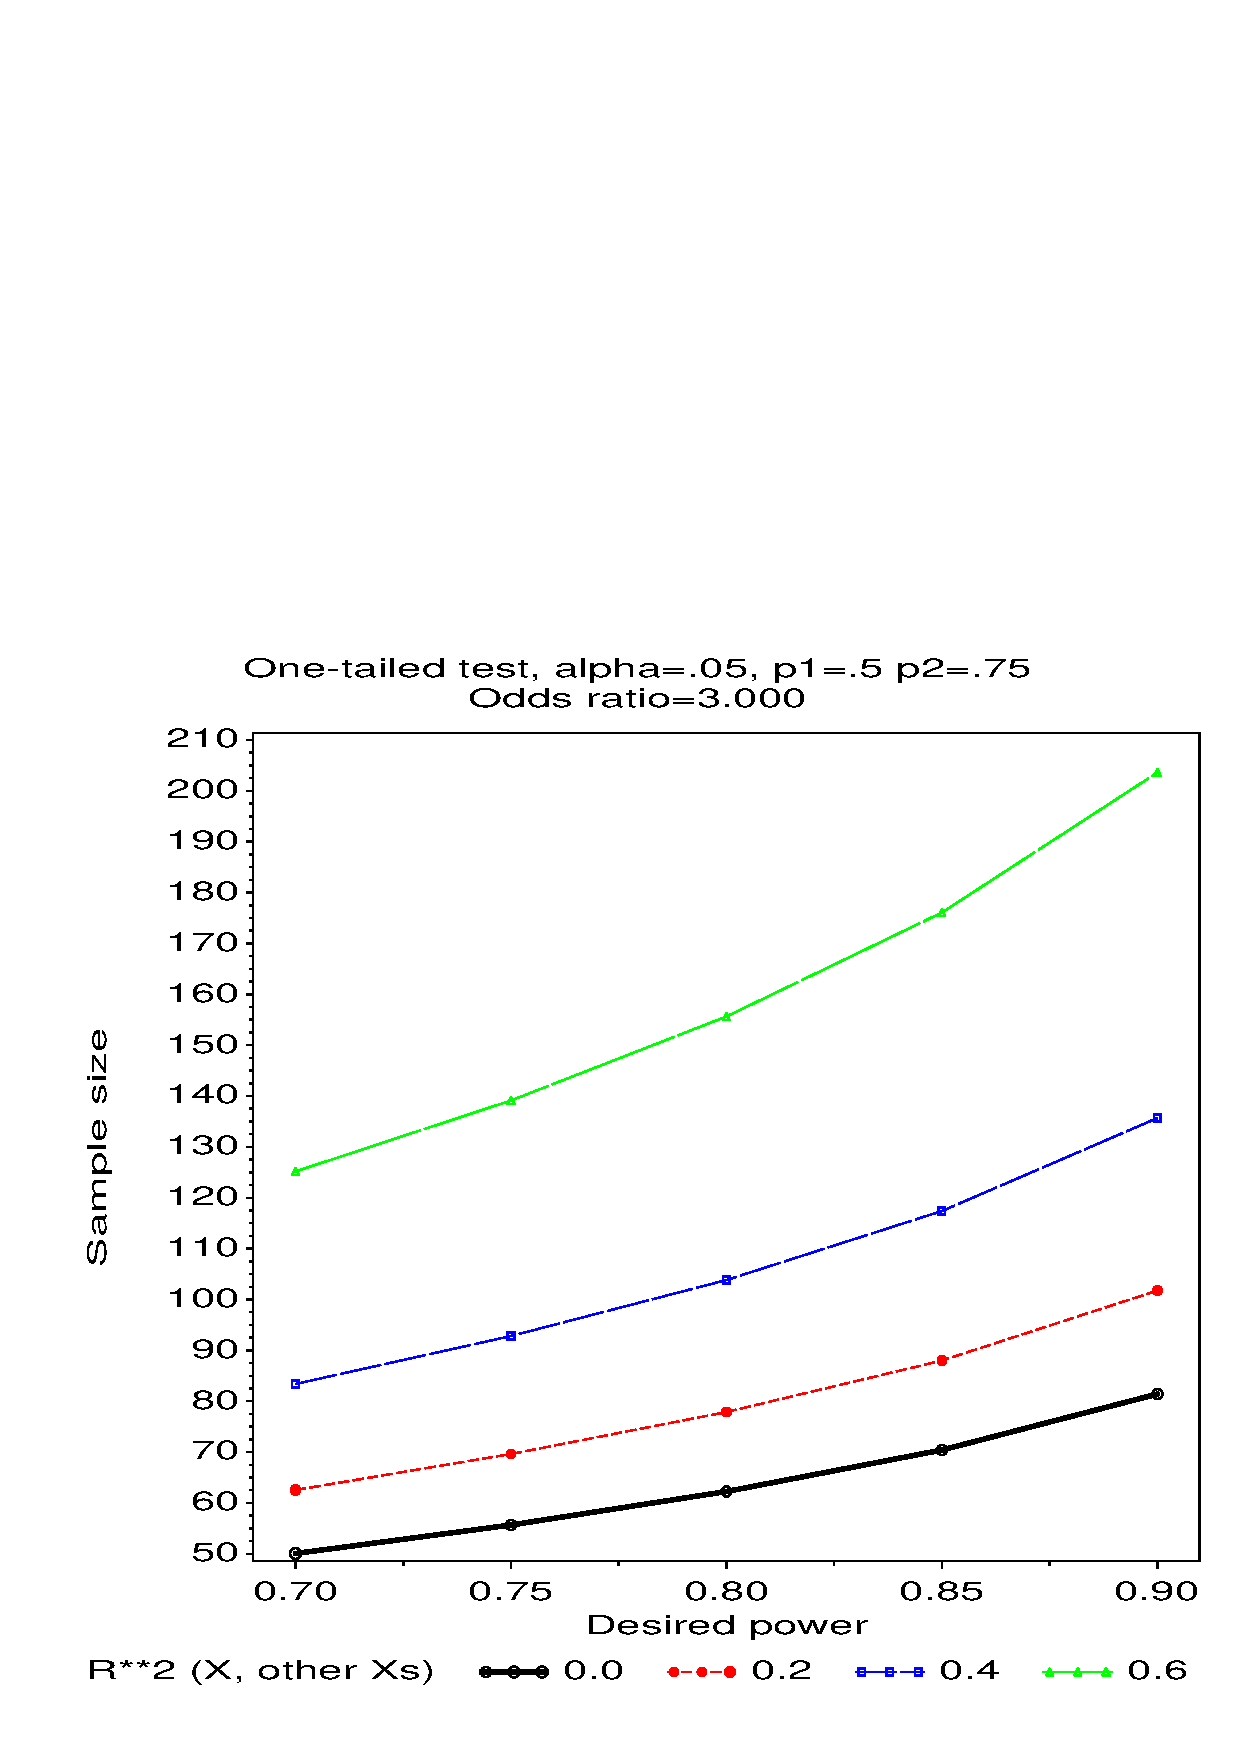
\includegraphics[scale=.6,clip]{ch6/fig/powerlog}
  \caption{Sample size display from \macro{POWERLOG}}%
  \label{fig:powerlog}
\end{figure}
\end{Example}



\section{Chapter summary}
\begin{itemize}
\item Model-based methods for categorical data provide confidence intervals
for parameters and predicted values for observed and unobserved values
of the explanatory variables.  Graphical displays of predicted values
help us to interprete the fitted relations and the models.

\item The logistic regression model describes the relationship between 
a categorical response variable, usually dichotomous,
and a set of one or more quantitative or discrete explanatory variables.
It is conceptually
convenient to specify this model as a linear model predicting
the log odds (or logit) of the probability of a success 
from the explanatory variables.

\item The relation between a discrete response and a quantitative predictor
may be explored graphically by plotting the binary observations 
and either the empirical log odds or equivalent probabilities
against the predictor, together with some smoothed curve.
The \macro{LOGODDS} provides some useful plots;
the \pname{SM}\emph{nn} spline smoothers available with the \stmt{SYMBOL}{GPLOT} in 
\PROC{GPLOT}
provide others.

\item For both quantitative and discrete predictors, the results of
a logistic regression are most easily interpreted from plots of
the predicted probabilities against the predictors
(or of log odds with an auxiliary scale of probabilities).
Confidence intervals or standard error bars provide a visual indication
of the precision of the predicted results.

\item When there are multiple predictors, effect plots (\secref{sec:logistic-effplot}) provide one method for constructing
simplified displays.

\item Influence diagnostics assess the impact of individual cases or
groups on the fitted model, predicted values, and the coefficients of individual predictors.  The \macro{INFLOGIS} 
and the \macro{ADDVAR} produces a variety of useful
plots designed to make these methods available for routine use.


\item Polytomous responses may be handled in several ways with
logistic regression.
The \emph{proportional odds model} is simple and convenient, but its validity
depends
on an assumption of equal slopes for adjacent-category logits.
\emph{Nested dichotomies} among the response categories give a set of models
which may be regarded as a single, combined model for the polytomous
response.
\emph{Generalized logits} may be used to construct models comparing
any pair of categories.

\item The basic logistic regression model may be applied in a wide
variety of related situations.  We illustrate its use in fitting
and graphing a model for paired comparisons.

\item Power analysis is an important adjunct to any statistical hypothesis
test, but depends on being able to specify a minimal effect size of
substantitive interest.
For the cases of a single binary predictor and a quantitative predictor
(possibly along with others), we describe the calculation of power or
required sample size, along with macro programs to provide tabular and
graphical displays.
\end{itemize}
